\documentclass[11pt]{book}

\usepackage{kotex} % korean tex
\usepackage{float}
\usepackage{longtable}
\usepackage[bookmarks]{hyperref}
\usepackage[utf8]{inputenc} % set input encoding (not needed with XeLaTeX)
\usepackage{listings}
\lstset{language=[90]Fortran,
  basicstyle=\ttfamily,  
  %basicstyle=\small,
  keywordstyle=\color{red},
  commentstyle=\color{green},
  morecomment=[l]{!\ }% Comment only with space after !
}

\usepackage{geometry} % to change the page dimensions
\geometry{letterpaper} % or letterpaper (US) or a5paper or....
% \geometry{margins=2in} % for example, change the margins to 2 inches all round
% \geometry{landscape} % set up the page for landscape
%   read geometry.pdf for detailed page layout information

\usepackage{graphicx} % support the \includegraphics command and options

% \usepackage[parfill]{parskip} % Activate to begin paragraphs with an empty line rather than an indent

\usepackage{booktabs} % for much better looking tables
\usepackage{array} % for better arrays (eg matrices) in maths
\usepackage{paralist} % very flexible & customisable lists (eg. enumerate/itemize, etc.)
\usepackage{verbatim} % adds environment for commenting out blocks of text & for better verbatim
\usepackage{subfig} % make it possible to include more than one captioned figure/table in a single float
% These packages are all incorporated in the memoir class to one degree or another...

%%% HEADERS & FOOTERS
\usepackage{fancyhdr} % This should be set AFTER setting up the page geometry
\pagestyle{fancy} % options: empty , plain , fancy
\renewcommand{\headrulewidth}{0pt} % customise the layout...
\lhead{}\chead{}\rhead{}
\lfoot{}\cfoot{\thepage}\rfoot{}

%%% SECTION TITLE APPEARANCE
\usepackage{sectsty}
\allsectionsfont{\sffamily\mdseries\upshape} % (See the fntguide.pdf for font help)
% (This matches ConTeXt defaults)

%%% ToC (table of contents) APPEARANCE
\usepackage[nottoc,notlof,notlot]{tocbibind} % Put the bibliography in the ToC
\usepackage[titles,subfigure]{tocloft} % Alter the style of the Table of Contents
\renewcommand{\cftsecfont}{\rmfamily\mdseries\upshape}
\renewcommand{\cftsecpagefont}{\rmfamily\mdseries\upshape} % No bold!

\usepackage{amsmath}
\usepackage{amssymb}
\usepackage{epsfig}
\usepackage{color}
\parindent 10pt\textheight 9in\topmargin -0.4in\textwidth 6in
\oddsidemargin .25in\evensidemargin 0in
\def\bm{\boldsymbol}
\def\vh{{\bm h}}
\def\vp{{\bm p}}
\def\vq{{\bm q}}
\def\vk{{\bm k}}
\def\vl{{\bm l}}
\def\vx{{\bm x}}
\def\vy{{\bm y}}
\def\vv{{\bm v}}
\def\vr{{\bm r}}
\def\vR{{\bm R}}
\def\la{\langle}
\def\ra{\rangle}

\newcommand{\bea}{\begin{eqnarray}}
\newcommand{\eea}{\end{eqnarray}}
\newcommand{\be}{\begin{eqnarray}}
\newcommand{\ee}{\end{eqnarray}}
\newcommand{\no}{\nonumber \\}
\newcommand{\nnb}{\nonumber}
\newcommand{\etal}{{\it et al.}~}
\newcommand{\eg}{{\it e.g.}}
\newcommand{\ie}{{\it i.e.}}
\newcommand{\sll}[1]{#1\hspace{-0.5em}/}
\newcommand{\del}{\partial}
\newcommand{\threejsymbol}[6]{\left(\begin{tabular}{ccc} {$#1$}&{$#2$}&{$#3$}\\
                             {$#4$}&{$#5$}&{$#6$}\end{tabular}\right)}
\newcommand{\sixjsymbol}[6]{\left\{\begin{tabular}{ccc} {$#1$}&{$#2$}&{$#3$}\\
                             {$#4$}&{$#5$}&{$#6$} \end{tabular}\right\}}
\newcommand{\ninejsymbol}[9]{\left\{\begin{tabular}{ccc}
                             {$#1$}&{$#2$}&{$#3$}\\
                             {$#4$}&{$#5$}&{$#6$}\\
                             {$#7$}&{$#8$}&{$#9$}\end{tabular}\right\}}
\newcommand{\threeDmat}[9]{\left(\begin{tabular}{ccc}
		{$#1$}&{$#2$}&{$#3$}\\
		{$#4$}&{$#5$}&{$#6$}\\
		{$#7$}&{$#8$}&{$#9$}\end{tabular}\right)}
%%% The "real" document content comes below...

\title{Scattering Theory Note: Reaction(FRESCO를 중심으로.)}
\author{Young-Ho Song}
\date{\today}
%\date{} % Activate to display a given date or no date (if empty),
         % otherwise the current date is printed 

\begin{document}
\maketitle
\tableofcontents
\newpage

\chapter{Direct Reaction theory} 

Basic notation of reaction,
When projectile $a$ collides with target $A$, and produce heavy remnant $X$
and ejectiles $x_1,\dots$, we denote
this reactions as
\bea 
A(a,x_1 x_2\dots)X.
\eea  
When particle is excited denote it as $A^*$. When projectile lose its 
kinetic energy denote it as $a'$. In many case, only the energy of projectile and ejectile are measured. 

실제 Reaction은 많은 경우, Binary reaction이고, Entrance Channel에서 
mass $m_a$, spin $s_a$ 인 projectile 을 mass $m_A$, spin $I_A$인 Target
과 충돌시킨 뒤 $m_b$,$s_b$ 와 $M_B$, $I_B$ 인 핵이 angle $\theta$ 방향으로 
얼마나 생성되는 지를 알고싶다. 따라서, 보통 Lab frame에서의 projectile kinetic energy를 
input으로 한다.  반면, 일반적으로 이론 계산은 C.M. frame 에서 계산하는 것이
편하므로, 먼저, input을 C.M. frame 에서의 양으로 변환하고, 이론적으로 계산한뒤, 
다시 Lab frame에서의 결과로 변환해 주어야 한다. 

\section{Reaction의 종류} 
\begin{figure}
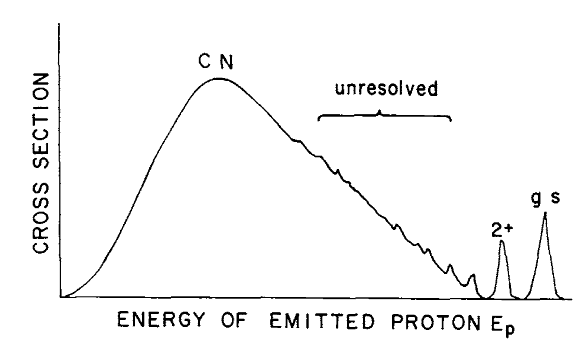
\includegraphics[width=0.5\linewidth]{Glend_fig1_1}
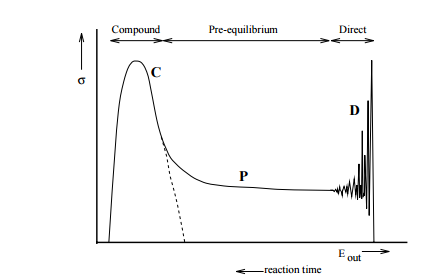
\includegraphics[width=0.5\linewidth]{talys_fig3_2}
\caption{Reaction cross section for proton scattering. 
proton scattering 이 반드시 elastic scattering을 의미하지는 않는다. 
그림에서 g.s.로 표시된 부분만이 elastic scattering에 해당한다. 	
주의할 것은 x축이 emitted particle energy라는 것이다.(즉, x축은 $E-E_{ex}$ 로 생각할 수있다.)
$E_p$가 낮을 수록 남은 핵이
높은 에너지 상태에 있게되어 available level density가 높아진다. 이 경우에는 
통계적인 관계식, Maxwell distribution을 잘 따르게 된다. 반면, $E_p$가 높으면,
남은 핵의 에너지가 낮은 에너지 상태가 되어 각각의 resonance등의 level이 중요하게 된다.
여기서 낮은 에너지 쪽은 Coulomb에 의해 Maxwell distribution으로부터 distorted 되어 있다. 
}
\label{fig:Glend_fig1_1}
\end{figure}

\begin{figure}
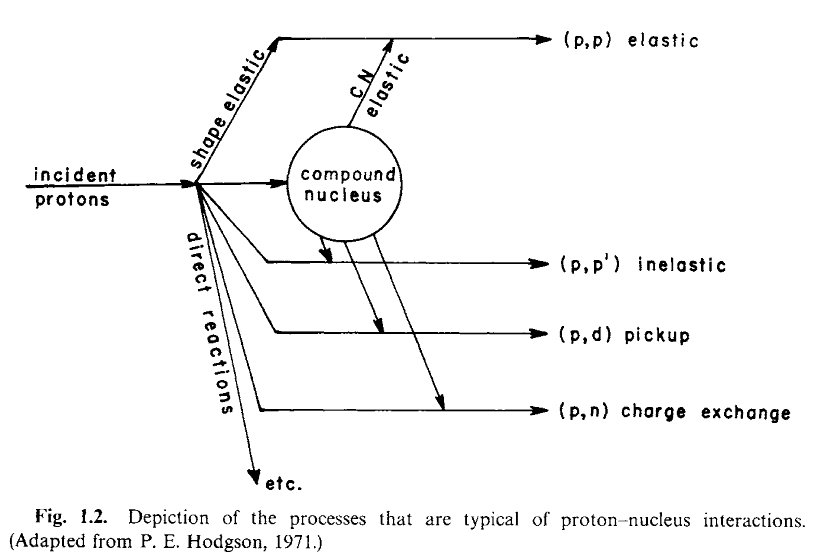
\includegraphics[width=0.5\linewidth]{Glend_fig1_2}
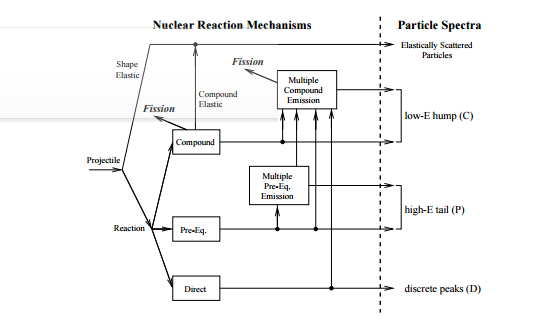
\includegraphics[width=0.5\linewidth]{talys_fig3_1}
\caption{Competition between reactions for proton scattering.
Note that compound nucleus can contribute any reaction channels. 
}
\label{fig:Glend_fig1_2}
\end{figure}

\begin{figure}
	\centering
	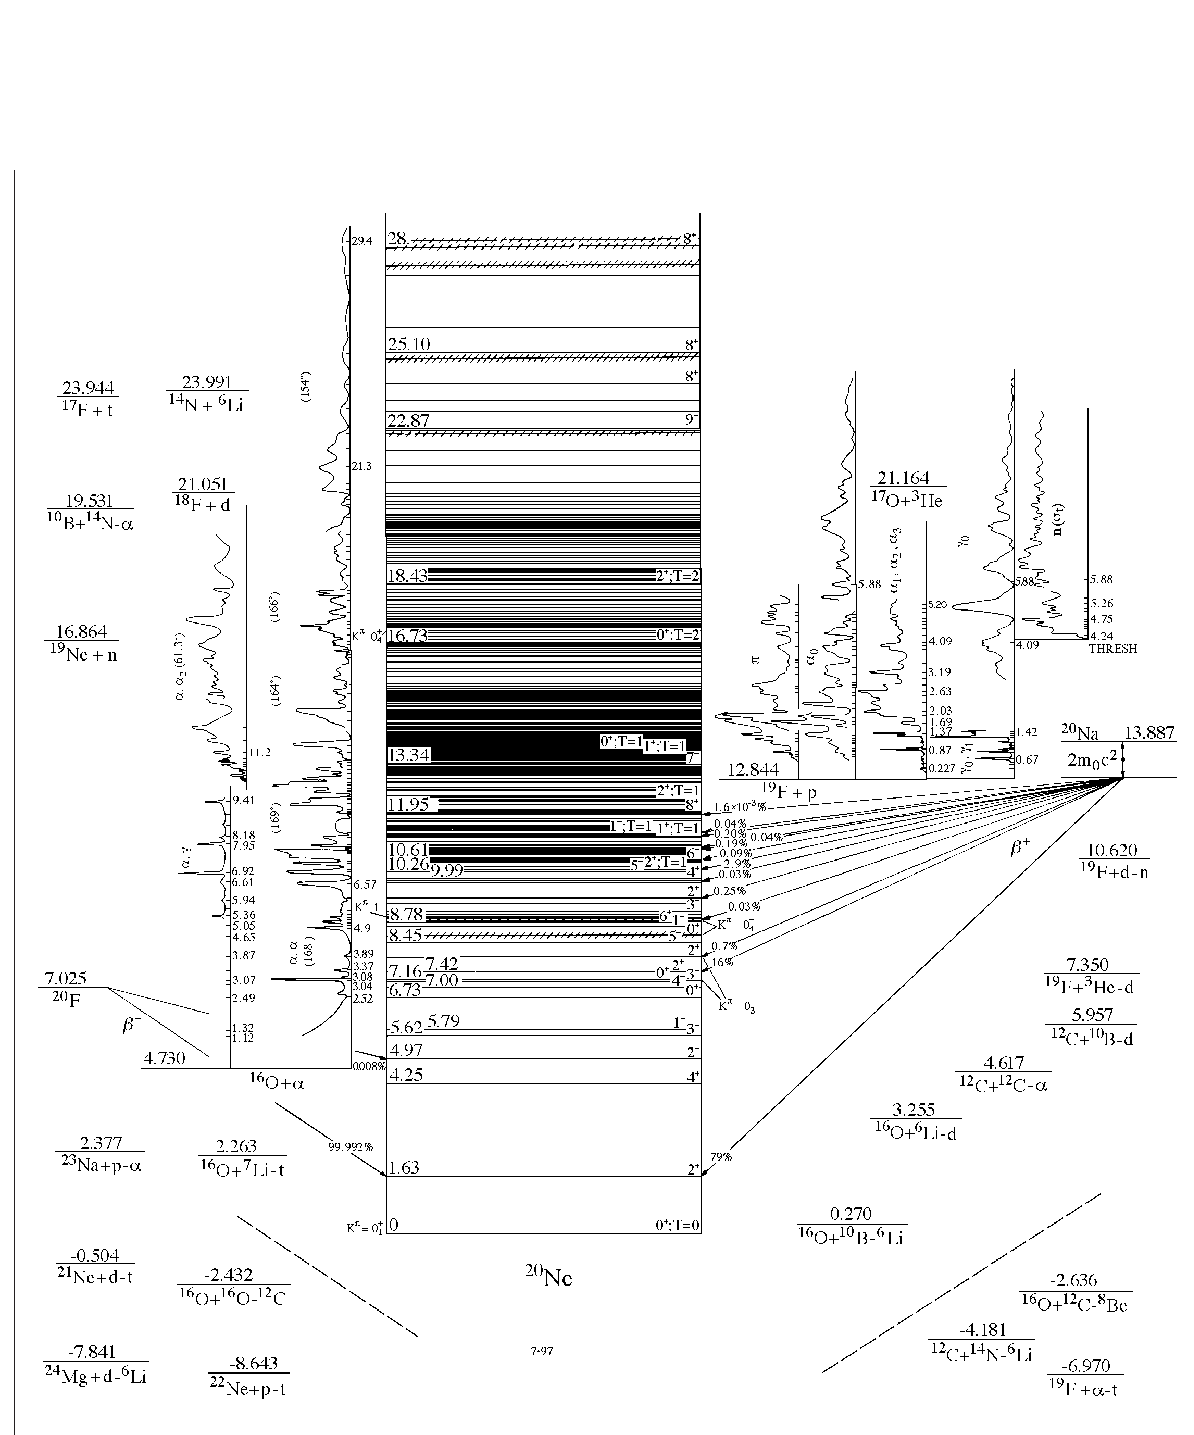
\includegraphics[width=0.8\linewidth]{Ne20}
	\caption{An Example of Energy levels. (Ne20 case).
	      Consider the scattering of $^{16}O+\alpha$.
          Near threshold only several energy levels of $^{20}Ne$ are relevant.
          On the other hand, as increasing energy of scattering,
          very dense resonance states become relevant. In this case, 
          statistical method should be used.  
           }
	\label{fig:ne20}
\end{figure}

\begin{figure}
	\centering
	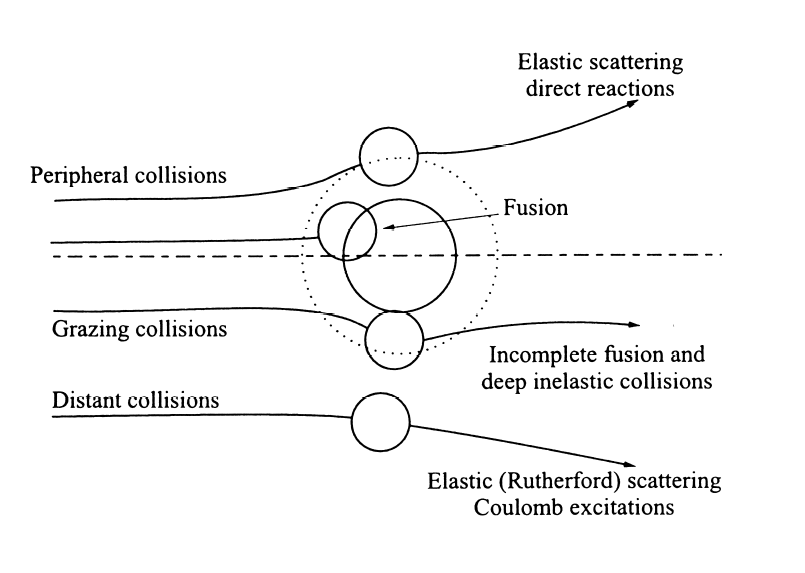
\includegraphics[width=0.7\linewidth]{HI_reaction_impact_para}
	\caption{Various Heavy ion reaction depending on the impact parameter}
	\label{fig:hireactionimpactpara}
\end{figure}


Direct Reaction
\begin{itemize}
\item Elastic scattering, $A(a, a)A$ : projectile and target stay in their g.s.
       , zero Q-value, no internal structure change.
       Usually the projectile angular distribution is measured. 
       
\item Inelastic scattering, $A(a,a')A^*$ or $A(a,a^*)A^*$:
projectile or target left in excited state. Projectile 
gives up some of its energy to excite target nucleus A. If
nucleus a also complex nucleus, it can also be excited.
[If energy resolution in detection of a not small enough to
resolve g.s. of target from low-lying excited states then cross
section will be sum of elastic and inelastic components. This
is called {\bf quasi-elastic scattering}].

Usually the projectile angular distribution is measured with momentum/energy. 

\item Transfer reaction, $A(a,b)B$ :
1 or more nucleons moved to the other nucleus. Stripping or Pickup. 


\item Fragmentation/Breakup/Knockout:
3 or more nuclei/nucleons in the final state

Usually referring to breakup of projectile
a into two or more fragments. This may be elastic breakup or
inelastic breakup depending on whether target remains in
ground state.

In case of knockout reaction(in narrow definition)
, the projectile fragments into a core and a nucleon
and the momentum of core particle is measured 
(target or fragment nucleon is not measured) with the gamma-ray emission
measuring coincidences with decay gamma-rays emitted in flight.
The momentum distribution gives the information of angular momentum and
spectroscopic factor.
(Difference between stripping and knockout? both refers a nucleon
is removed from projectile. In case of stripping or inelastic breakup,
the removed nucleon interacts with the target. But, in diffractive or
elastic breakup, a nucleon is dissociated elastically? )
Because only core is observed, both contribution
of stripping and elastic breakup have to be summed.

MOMDIS code describes reaction $(c+v)+T\to c+X$.

\item Charge Exchange:
A is constant but Z (charge) varies, e.g. by pion exchange.
mass numbers remain the
same. Can be elastic or inelastic. It can occur in many ways. 
(1) directly changing the charge of both projectile and target. 
    ($\Delta T=1$ transition both in target and projectile)
(2) knocking out one nucleon and replacing the projectile.
    ($\Delta T=0$ transition vertex but exchanging two particles.
    In effect, the nuclear transition will be $\Delta T=1$ though the
    vertex is $\Delta T=0$.
    )   
(3) In a two step process by absorbing and emitting particles between target
    and projectile.      

\item Multistep Processes:
intermediate steps can be any of the above
(`virtual' rather than `real')
\end{itemize}


Compound Reaction
\begin{itemize}
\item Deep inelastic collisions:
Highly excited states produced
\item Fusion:
Nuclei stick together
\item Fusion-evaporation:
fusion followed by particle-evaporation and/or gamma
emission
\item Fusion-fission:
fusion followed by fission

\end{itemize}

Coumpound Reaction과 Direct reaction의 차이
\begin{itemize} 
\item 
Nuclei can coalesce to form highly excited Compound
nucleus (CN) that lives for relatively long time.
Long lifetime sufficient for excitation energy to be shared by
all nucleons. If sufficient energy localised on one or more
nucleons (usually neutrons) they can escape and CN decays.
Independence hypothesis: CN lives long enough that it loses
its memory of how it was formed. So probability of various
decay modes independent of entrance channel.

Nuclei make `glancing' contact and separate immediately, said
to undergo Direct reactions(DI).
Projectile may lose some energy, or have one or more nucleons
transferred to or from it.

\item Reaction이 일어나는 위치에 따라서 구분:
CN reactions at small impact parameter,
DI reactions at surface and large impact parameter.
CN reaction involves the whole nucleus.
DI reaction usually occurs on the surface of the nucleus. This leads
to diffraction effects.

\item Reaction에 걸리는 시간에 따라서 구분:

A typical nucleon orbits within a nucleus with a period of $10^{-22}$
sec. [as K.E. $\sim$ 20 MeV].
If reaction complete within this time scale or less then no time for
distribution of projectile energy around target ) DI reaction
occurred. CN reactions require $10^{-22}$ sec.

\item Angular Distribution:
In DI reactions differential cross section strongly forward peaked as
projectile continues to move in general forward direction.
Differential cross sections for CN reactions do not vary much with
angle (not complete isotropy as still slight dependence on direction
of incident beam).

\end{itemize}

Direct reactions at low energies need extra care. Are such energies high enough and timescales short
enough for reactions to be fast and direct?

Let us consider an example of neutron incident reaction for different incoming neutron energies.
\begin{itemize}
\item Low energies (E$<$0.2 MeV): Elastic scattering and capture. Since at low energy below 1st excited state of target, only possible reactions are (1) elastic scattering (2) capture (3) fission if target is fissible. 
\item Low energies (0.2$<$E$<$ 4 MeV) : Inelastic scattering to discrete states. 
  All reactions in previous energy are available and Compound reactions contributes to 
  all channels.  When the
  incident energy crosses an inelastic threshold, the compound inelastic contribution rises rapidly and predominates,
  whereas the direct component increases more gradually.
\item High energy (E$>$4 MeV): Pre-equilibrium reactions. 
  reactions to the continuum also have a compound and a direct-like component.
  The latter are usually described by pre-equilibrium reactions which, by
  definition, include direct reactions to the continuum. 
  Non-elastic channels contribute. 
\item High energy(E $>$8 MeV): Multiple compound emission. At incident energies above about the neutron separation energy, the residual nuclides formed after the
first binary reaction contain enough excitation energy to enable further decay by compound nucleus
particle emission or fission. 
\item High energy (E$>$40 MeV): Multiple pre-equilibrium emission. At still higher incident energies, above several tens of MeV, the residual nuclides formed after binary
emission may contain so much excitation energy that the presence of further fast particles inside the
nucleus becomes possible. 
\end{itemize}

\section{핵반응에서 측정하는 물리량}
\begin{itemize}
\item 탄성산란의 미분단면적 : projectile energy(de Broglie wave length) and the size of the target
      affects the angle dependence of the cross section. Using this information, we can indirectly
      infer the average strength of interaction, the size of target.
      (Optical potential fit may have physical relevance with the radius and diffuseness of
      the target)
\item Total reaction cross section : 입자의 핵에의 흡수정도를 나타내고, 상호작용의 크기와 핵의 크기에 대한 정보를 준다. 
\item Inelastic scattering cross section: 각운동량에 민감하다. 핵의 들뜲상태의 에너지, 각운동량, 패리티등에 대한 정보를 준다. 산란된 입자이외에도 방출된 gamma 나 전자를 동시에 측정하는 경우 더 자세한 정보를 얻을 수 있음. 
\item rearrangement reaction의 미분 산란 단면적: transfer, fusion 등등. one nucleon transfer reaction can be used to extract information for a single particle state. Two nucleon transfer can be used to
extract the correlation of two nucleons. 
\item 편극량 측정: spin dependence of cross section gives more information on the nuclear interaction. 입사 입자, 표적, 산란입자의 스핀에 대한 의존도를 측정할 수 있다.  
\end{itemize}

\section{Conservation laws in nuclear reaction} 
\begin{itemize}
\item Energy-Momentum Conservation
\item (total) Angular momentum Conservation
\item (approximate) Parity
\item (electric) Charge
\item (approximate) Isospin
\end{itemize}

\section{Reaction Theory 기본 용어}
이제 부터는 Direct Reaction 의 경우만 생각하자. 


For process,
\bea 
p(proj)+T(target)\to x+R(remnant),\quad \rightarrow T(p,x)R.
\eea 
의 반응의 Q-value 는
\bea 
Q=(m_p+m_T-m_x-m_R)c^2, 
\eea 
으로 최종 products에서 available한 운동에너지에 해당한다. 이때 가능한 최종 product가 
여러가지인 경우를 생각할 수 있다. 

\begin{itemize}
	\item In standard nuclear reaction, the number of nucleons does not change
	and the target is at rest. 
	Thus, in non-relativistic limit, we can rephrase,
	$Q=T_x+T_R-T_p$.
	\item One necessary condition for the reaction occur is $Q+T_p>0$.
	      Further constraint is $T_p \geq -Q\frac{m_p+m_T}{m_T}$.
	\item Mass excess $\Delta$: difference between actual mass and atomic mass unit times atomic number. 
	     $m_A= A m_{amu}+\Delta$. 
	\item In fact, Q-value can be determined by measuring ejectile energy $T_x$ and angle $\theta_x$
	  from Q-equation:   
	  \bea 
	  Q= T_x(1+\frac{m_x}{m_R})-T_p(1-\frac{m_p}{m_R})-\frac{2}{m_R}\sqrt{m_p T_p m_x T_x}\cos\theta_x 
	  \eea    
\end{itemize}



\section{Direct Reaction channel} 
예를 들어서, 3 개의 입자, $a,b,c$ 로 이루어진 시스템을 생각해보자. Initially, b와 c가 bound state
$(bc)$ 를 만들수 있다고 하자. $a+(bc)$ 의 반응에서 일어날 수 있는 경우가 다음과 같다고 하자.
\bea 
a+(bc) &\to a+b+c , &\mbox{0(break up)},\no 
       &\to a+(bc), &\mbox{1(elastic)},\no 
       &\to a+(bc)^*,&\mbox{2(inelastic)},\no 
       &\to (ab)+c ,&\mbox{3(transfer)},\no 
       &\to (abc) ,&\mbox{4(capture)} 
\eea 
이와 같이 가능한 구분 가능한 최종 product들(1,2,3,4)을 channel 이라고 부르고, 
이 중 particle들의 구성만으로 구분하는 것을 partition 이라고 부른다.(0,1,3,4 는
모두 다른 partition이지만, 1과 2는 같은 partition이다.)
Each partition further distinguished by state of excitation of each
nucleus and each such pair of states is known as a "{\bf reaction
channel}".
The initial partition is known
as the incident, or entrance channel and various possible
outcomes are the possible exit channels.
In a particular reaction, if not enough energy for a particular exit
channel then it is said to be closed.

보통 channel이라는 말을 reaction channel과 각 reaction channel의 partial wave form을 
구분하지 않고 사용한다. 그러나, 여기서는 되도록, reaction channel과 partial wave channel을 
구분하여 사용하도록 하자. reaction channel은 각 channel의 energy, partition 그리고, 
spin states 를 나타내고, partial wave channel은 각 reaction channel을 partial wave expansion 
하여 angular momentum 까지 정해지는 상태를 나타낸다. 

\begin{itemize} 
\item Direct reaction 계산에서는 각 channel $\alpha$에서의 wave function이 
projectile wave function($\phi_p$), target wave function($\phi_t$) 
그리고 이 둘의 relative wave function $\psi_\alpha(R)$
으로 주어진다고 가정하고, 이 때의 exit channel의 relative wave function을 구하면 
differential cross section등을 얻을 수 있다. 
\bea 
\mbox{(channel wave function)}= [\phi_p\otimes \phi_t]_\alpha \psi_\alpha(R)
\eea  

Target과 Projectile의 bound state wave function이 
알려져 있다고 가정할 때, 필요한 것은 Schrodinger equation으로 부터 
각 channel의 relative wave function을 구하는 것이다. 
한편, 이러한 relative wave function들이 만족해야 하는 식은 
각 channel 사이의 coupling을 가지는 coupled equation이 된다. 

\item cross section: DWBA에서는 bound state wave function과 distorted wave function이 
      이미 알려져 있다고 생각하고 T-matrix를 potential과 wave function에 대한 integral 로 계산한다. 한편, CC 에서는 bound state wave function은 이미 알려져 있다고 가정하지만,
      distorted wave를  coupled equation을 풀어서 구하게 된다. 따라서, 이경우에는 
      얻어진 wave function으로부터 T-matrix 또는 S-matrix 를 구하고, 이를 이용해서
      cross section을 계산한다. 그러므로, multi-channel T-matrix또는 S-matrix와 
      cross section을 연결시키는 식이 필요하다.       
\end{itemize}

따라서, 계산은 

(1) Obtain distorted wave for channels either by solving coupled equation.

(2) Compute T-matrix either from Asymptotic form of 
    distorted wave from coupled equation or by computing DWBA matrix elements
    
(3) Compute Differential Cross section from T-matrix.     

\begin{itemize} 
\item 예를 들어서 x 라는 partition의 target 과 projectile 있을 때, 이 partition이 
$J_{tot},M_{tot}$을 가질 때 wave function 은  아래와 같이 
나타 낼 수 있다.
\bea 
\Psi_{x,J_{tot}}^{M_{tot}}(R_x,\xi_p,\xi_t)
&=&\sum_{\alpha} \left[ 
    \left[i^{L} Y_{L}(\hat{R}_x)\otimes \phi^{xp}_{I_p}(\xi_p)\right]_{J_p} 
    \otimes \phi^{xt}_{I_t}(\xi_t)\right]_{J_{tot}M_{tot}}
    \frac{1}{R_x}\psi_{\alpha}^{J_{tot}}(R_x) \no 
&=&\sum_{\alpha} |xpt:(L I_p) J_p,I_t;J_{tot} M_{tot}\ra 
    \frac{\psi_{\alpha}^{J_{tot}}(R_x) }{R_x} \no 
&=&\sum_{\alpha} |\alpha; J_{tot} M_{tot}\ra \frac{\psi_{\alpha}^{J_{tot}}(R_x) }{R_x}
\eea 
여기서 $\alpha=(x,p,t,L,I_p,J_p,I_t)$ 으로써, $|\alpha; J M\ra $는 $J_{tot},M_{tot}$ 을 
만드는 모든 channel들을 나타내고, bound state wave function 즉 internal structure를 포함한다. 

\item 일반적으로 incident channel wave function 은 $J,M$ 의 eigen state가 아닌 
plane wave 이므로, 이 들을 각 $J,M$의 eigen state $\alpha_i$ 로 분해하고, 동시에 
반응후에 갈 수 있는 최종 channel $\alpha$ 의 합으로 나타내면,
\bea 
\Psi_{x_ip_it_i}^{\mu_{p_i}\mu_{t_i}}(R_x,\xi_p,\xi_t; \vk_i)
=\sum_{J_{tot}M_{tot}}\sum_{\alpha \alpha_i}
  |\alpha;J_{tot}M_{tot}\ra 
   \frac{\psi^{J_{tot}}_{\alpha \alpha_i}(R_x)  }{R_x} 
   A^{J_{tot} M_{tot}}_{\mu_{p_i}\mu_{t_i}}(\alpha_i,\vk_i)
\eea  
where, "incoming coefficient" is defined as
\bea 
A^{J_{tot} M_{tot}}_{\mu_{p_i}\mu_{t_i}}(\alpha_i,\vk_i)
=\frac{4\pi}{k_i}\sum_{M_i m_i} Y^*_{L_iM_i}(\vk_i)
  \la L_iM_i,I_{p_i} \mu_{p_i}| J_{p_i} m_i\ra 
  \la J_{p_i} m_i,I_{t_i}\mu_{t_i}|J_{tot} M_{tot}\ra. 
\eea  
incoming coefficient 는 plane incoming wave를 잘 정의된 incoming channel 들로 
변환시켜주고, 최종 wave function은 이 incoming channel들이 outgoing channel로 바뀐
결과들의 합이다. 
따라서, 우리가 필요한 것은 하나의 잘 정의된 incmoing channel로부터의 outgoing channel의 
wave function $\psi^{J_{tot}}_{\alpha \alpha_i}(R_x)$를 구하는 것이다. 

즉, 위 식에서 $\Psi_{x_ip_it_i}^{\mu_{p_i}\mu_{t_i}}(R_x,\xi_p,\xi_t; \vk_i)$는 
incident reaction channel
$|  x_i p_i t_i, \mu_{p_i} \mu_{t_i},\vk_i \ra $ 로부터 얻어지는
total system wave function 으로, 각 reaction channel로의 wave function의 합이다.
한편, $A^{J_{tot} M_{tot}}_{\mu_{p_i}\mu_{t_i}}(\alpha_i,\vk_i)$ 는 
incident channel을 partial wave decompose 시킬 때 나타나는 
partial reaction channe의 계수이다. 
한편, $\alpha;J_{tot}M_{tot}\ra$ 는 최종적으로 관찰되는 partial reaction channel을 
타나태고, $\psi^{J_{tot}}_{\alpha \alpha_i}(R_x)$는 
incident partial channel $\alpha_i$에서 final partial channel $\alpha$ 로의 
전이 확률을 나타내는 파동함수가 된다. 

Or, in combination,
\bea 
\Psi_{x_ip_it_i}^{\mu_{p_i}\mu_{t_i}}
= \sum \frac{4\pi}{k_i} i^{L} Y^*_{L_iM_i}(\vk_i) Y_{L}(\hat{R}_x)
    \frac{1}{R_x}\chi_{\alpha\alpha_i}^{J_{tot}}(R_x)
        (\mbox{C.G.'s})(\mbox{bound state waves})
\eea 
with $\psi$ is normalized as Coulomb wave function,
\bea 
\chi_{\alpha\alpha_i}(R_x)\to 
\frac{i}{2}[H_\alpha^{(-)}\delta_{\alpha\alpha_i}-S_{\alpha\alpha_i} H_\alpha^{(+)}]
\eea 
주의할 것은 $1/k$ 는 incoming coefficient에 포함되어 있었다는 것이다. 
\item 어떤 channel $\alpha$에서 target과 projectile의 bound state 를 
$\alpha p$, $\alpha t$ 라고 하자.마찬가지로 wave function은 
$\phi_{\alpha p}(\xi_{\alpha p})$ , $\phi_{\alpha t}(\xi_{\alpha t})$로 쓰고,
$\xi$는 bound state의 internal degree of freedom 을 나타낸다. 
\end{itemize}

\subsection{Wave functions}
To start with, the 
{\color{blue} excitation
energies, spins and parities of all the states in each mass partition} need to be specified, along
with 
{\color{blue}
the nuclear masses, charges and relative Q-values of the partitions. 
Each pair projectile
and target excited states is then a distinct channel with its own scattering wave function and  boundary conditions}. 
The initial projectile and target states will select one such channel as the
‘incoming channel’, with its boundary conditions specifying an incoming plane wave. 
All channels
(including the incoming channel) will have outgoing spherical waves. Particular attention
must be given to the consistent placement of $i^L$ factors in these definitions.

The individual nuclear states are then specified in sufficient detail for the particular reaction
mechanisms involved. 
It is not necessary to specify the full quantum mechanical states of all
the nucleons in the nucleus, but rather, 
only the states of those changed in the reactions being
considered. 
In particular, {\color{blue} one and two-nucleon wave functions} will have to be described, if those
nucleons are to be transferred to other nuclei. 

If a nuclear state consists of a particle of spin s
bound outside a nucleus with possible core states $\phi_I$ , 
then the {\color{blue} bound state radial wave functions
$u_{lsjI}(r)$ will have to be found 
by solving a coupled-channels set of equations for negative energy
eigen-solutions}(즉, 여기서 $u$는 core-valence particle wave function). 

If the particle is not bound, in the other hand, then its continuum range of
energies must be discretized into a finite collection of {\color{blue} ‘bin’ states} which can be scaled to unit
normalisation. 

If the nuclear state consists of two particles of intrinsic spins 
$s_1$ and $s_2$ outside
a core, then it is usually specified by a shell-model 
or by a Sturmian-basis calculation in terms
of the independent coordinates $r_1$ and $r_2$. 
To calculate transfer rates, however, 
the {\color{blue} two-particle
wave functions} need to be given in terms of the collective coordinates 
(usually $\vr = \frac{1}{2}(\vr_1+\vr_2)$
and  $\rho= r_1 - r_2$). 
In order to use the states in a reaction calculation, therefore, equations are
given for the transformation from the independent coordinates.

\subsection{Optical Model}


\subsection{Cross section}
In case of multi-channel case, differential cross section for asymptotic wave
\bea 
\psi_{\beta}(\vk_\alpha)
 \to e^{i \vk_\alpha\cdot \vr_\alpha}\delta_{\alpha\beta}
        +f_{\beta\alpha}(\vk_\beta,\vk_\alpha)\frac{e^{i\vk_\beta\cdot \vR_\beta}}{R_\beta}
\eea 
gives flux,
\bea 
J_\alpha=\frac{\hbar k_\alpha}{\mu_\alpha},\quad 
\hat{J}_{\beta\alpha}=\frac{\hbar k_\beta}{\mu_\beta} |f_{\beta\alpha}|^2,
\eea 
with
\bea 
f_{\beta\alpha}(\theta)&=& -\frac{\mu_\beta}{2\pi\hbar^2}
                          \la e^{i\vk_\beta\cdot\vr_\beta}|V_\beta|\Psi^{(+)}_\alpha\ra
                          \no 
                        &=&-\frac{\mu_\beta}{2\pi\hbar^2} T_{\beta\alpha}(\vk_\beta,\vk_\alpha),   
\eea 
and cross section
\bea 
\frac{d\sigma_{\beta\alpha}}{d\Omega}&=&\frac{\mu_\alpha}{\hbar k_\alpha}
   \frac{\hbar k_\beta}{\mu_\beta}|f_{\beta\alpha}|^2 
   =(\frac{v_\beta}{v_\alpha})|f_{\beta\alpha}(\vk_\beta,\vk_\alpha)|^2 ,\no 
  &=&\frac{\mu_\alpha \mu_\beta}{(2\pi\hbar^2)^2}(\frac{k_\beta}{k_\alpha})
     | T_{\beta\alpha}(\vk_\beta,\vk_\alpha)|^2.
\eea 
단, 여기서, $(f,T)_{\beta \alpha}$는 아직 partial wave
expansion을 하지 않은 형태이다.

In other words,
\bea 
T=\la \vk_f; I_{p_f} M_{p_f} I_{t_f} M_{t_f}|V|\vk_i;I_{p_i} M_{p_i} I_{t_i} M_{t_i}\ra^{(+)} 
\eea 
In this form, $V$ contains every interaction in the Hamiltonian,
left state is a plane wave state and right state is a full solution of Hamiltonian. 
Each states includes bound state wave functions and wave function for relative motion.
Bra-ket implies the integration over all coordinates. 

Then, 
\bea 
\sigma_{xpt}(\theta)&=&\frac{1}{(2I_{p_i}+1)(2I_{t_i}+1)}
    \sum_{\mu_p\mu_t\mu_{p_i}\mu_{t_i}} 
    \frac{v_f}{v_i} 
    |f^{xpt}_{\mu_p\mu_t\mu_{p_i}\mu_{t_i}}|^2 \no 
    &=& \frac{1}{(2I_{p_i}+1)(2I_{t_i}+1)}
        \sum_{\mu_p\mu_t\mu_{p_i}\mu_{t_i}}  
        |\widetilde{f}^{xpt}_{\mu_p\mu_t\mu_{p_i}\mu_{t_i}}(\theta)|^2
\eea 
with 
\bea 
\widetilde{f}^{xpt}_{\mu_p\mu_t\mu_{p_i}\mu_{t_i}}(\theta)
&=& \delta_{\mu_p\mu_{p_i}}\delta_{\mu_t\mu_{t_i}}\delta_{xpt,x_ip_i t_i}
    f_c(\theta) \no 
  & &+\frac{4\pi}{k_i}\sum_{L_i M_i, L M}\sum_{J_{p_i} m_i, J_p m}  
     \sum_{J_{tot} M_{tot}}
     C_{ L_i M_i, I_{p_i}\mu_{p_i}}^{J_{p_i}m_i}
     C_{J_{p_i} m_i,I_{t_i}\mu_{t_i}}^{J_{tot}M_{tot}}
     C_{L M, I_{p}\mu_{p}}^{J_{p}m}
     C_{J_{p} m,I_{t}\mu_{t}}^{J_{tot}M_{tot}}
     \no & &\times 
     Y_{LM}(\hat{k})Y^*_{L_i M_i}(\hat{k}_i)
     \tilde{T}^{J_{tot}\pi}_{\alpha\alpha_i}
     e^{i\sigma_L(\eta_\alpha)+i\sigma_{L_i}(\eta_{\alpha_i})}     
\eea 
where 
\bea
\tilde{T}^{J_{tot}\pi}_{\alpha\alpha_i}
=\frac{i}{2}[\delta_{\alpha\alpha_i}-\tilde{S}^{J_{tot}\pi}_{\alpha\alpha_i}]
\eea 
with
\bea 
\tilde{S}^{J_{tot}\pi}_{\alpha\alpha_i}
=\sqrt{\frac{v_\alpha}{v_{\alpha_i}}}S_{\alpha\alpha_i}
\eea 
Note that usual $i^{L-L_i}$ factor is included into the coupling potential,
and thus into the definition of $T$-matrix 
by the combination with bound state wave. 

Or, 
\bea 
\widetilde{f}^{xpt}_{m' M';m M}(\theta)
= \delta_{\alpha\beta}f_c(\theta)
 +\sum_{L'} A^{L'}_{m' M';m M} P_{L'}^{m'+M'-m-M}(\cos\theta) 
\eea 
where
\bea 
A^{L'}_{m'M';mM}&=& \sum_{LJJ' J_T} C^{Jm}_{L0 J_p m} C^{ J_T M_T}_{J m J_t M}
                            C^{J' M_{L'}+m}_{L' M_{L'} J'_{p} m'}
                            C^{J_T M_T}_{J' M_{L'}+m' J'_t M'}
                            \no & & \times 
                            \frac{4\pi}{k_i}\sqrt{\frac{k'\mu}{\mu' k}}
                            e^{i\sigma_L}e^{i\sigma'_{L'}}
                            \frac{i}{2}\left[\delta_{\alpha\alpha'}-S^{J_T}_{\alpha'\alpha}\right]
                            \sqrt{\frac{2L+1}{4\pi}}Y_c(L',M_{L'})
\eea 
where $Y_{c}(L,M)$ is the coefficient of $P^{|M|}_{L}(\cos\theta)e^{iM\phi}$ in $Y_{LM}(\theta,\phi)$




In the last expression, $T_{\alpha\alpha_i}$ is expressed in partial wave form.
Thus, in practice, it implies
\bea 
T_{\alpha\alpha_i}&=&
\la k_\alpha, \alpha \phi_\alpha | V_\beta| k_{\alpha_i}, \alpha_i,\phi_\alpha\ra^{(+)}\no 
| k_{\alpha_i}, \alpha_i,\phi_\alpha\ra^{(+)}
&=&\sum_{\alpha'} |\alpha',\phi_{\alpha'}\ra \frac{\chi_{\alpha\alpha_i}^{(+)}(R_{\alpha'})}{R_{\alpha'}},\no
|k_\alpha, \alpha \phi_\alpha \ra
&=& |\alpha,\phi_{\alpha}\ra j_\alpha(R_\alpha).
\eea 
here, the wave function $\chi_{\alpha\alpha_i}^{(+)}$ is a full 
solution of full Schrodinger equation. Also, note that the expression
implies the integral over all relevant coordinates. But, usually, the T-matrix
is inferred from the boundary condition of full wave function
instead of the integral over potential. 

In case of DWBA, ($\alpha\neq \alpha_i$), the T-matrix 
is computed by the integral over potential, 
\bea 
T^{DW}_{\alpha\alpha_i}&=&
{}^{(-),DW}\la k_\alpha, \alpha \phi_\alpha | V_\beta | k_{\alpha_i}, \alpha_i \phi_{\alpha_i}\ra^{(+),DW},\no 
| k_{\alpha}, \alpha,\phi_\alpha\ra^{(\pm),DW}
&=&\sum_{\alpha'} |\alpha',\phi_{\alpha'}\ra \frac{\chi_{\alpha'\alpha}^{(\pm),DW}(R_{\alpha'})}{R_{\alpha'}}.
\eea 
where $\chi_{\alpha'\alpha}^{(\pm),DW}$ is a solution of 
Schrodinger equation with optical potential. In many case, the optical potential
is diagonal, $\chi_{\alpha'\alpha}^{(\pm),DW}
=\delta_{\alpha\alpha'} \chi_{\alpha}^{(\pm),DW}$. 

\subsubsection{Additional terms} 
\begin{itemize}
	\item Consider beam intensity $\phi$ particles/sec with beam area A cm$^2$. After passing target
	with thickness $dx$, beam intensity will change as $\phi+d\phi$. 
	
	Usually, beam intensity of charged particle is written in terms of current(micro Ampere, $\mu A$). 
	
	For example, 1$\mu A$ proton is 
	\bea 
	\phi = (1\mu A)\times \frac{10^{-6} Coul/sec}{\mu A} \times \frac{1}{1.602\times 10^{-19} Coul/proton}
	=6.24 \times 10^{12} protons/sec
	\eea 
	Or, one can use (particle microamperes)$=6.24 \times 10^{12}$ ions/sec.
	
	\item Assume change of intensity is from the blocking of target nuclei. Then the ratio of 
	$\phi$ and $d\phi$ will be related with the ration of beam area and effective area covered by 
	all target nuclei. Number of all target nuclei is $\rho dx A$. Let effective area of one nuclei
	as $\sigma_{tot}$.      
	\bea 
	\frac{-d\phi}{\phi}=\frac{\rho dx A \sigma_{tot} }{A}= \rho \sigma_{tot} dx
	\to \phi(x) =\phi_0 e^{-\rho \sigma_{tot} x}.
	\eea 
	Usually, target density is written in terms of N atoms/cm$^2$ for a very thin target 
	instead of $\rho$ atoms/cm$^3$.  	
	\item Number of product nuclei, $d N_{p}$,  during time $t$ passing $dx$ can be computed as 
	\bea 
	d N_{p}=\phi(x)(1-e^{-\rho \sigma_{tot} dx}) t. 
	\eea 
	If the product is radioactive and decay, change of number of product in time is 
	\bea 
	& &\frac{ d N_p}{dt}=(\mbox{production rate})-(\mbox{decay rate})
	= \rho \sigma_{tot} dx \phi -\lambda N_p \no 
	&\Rightarrow& \frac{dN_p}{\rho \sigma_{tot} dx \phi -\lambda N_p}=dt                 
	\eea 
	We may introduce $A$ as the disintegration rate of product nuclei at the end of the irradiation.
	\bea 
	A=\rho \sigma\Delta x \phi (1-e^{-\lambda t}) 
	\eea 
	Number of product nuclei at the end of irradiation is $A/\lambda$, or 
	\bea 
	N=\frac{\rho \sigma\Delta x \phi}{\lambda} (1-e^{-\lambda t}) 
	\eea 
	\item Classically we can view total cross section as $\sigma_{tot}\simeq \pi r_0^2(A_P+A_T)^2$.
	  In semi-classically, to get a contribution from a particular orbital angular momentum, 
	  we may use impact parameter $l=bp$ and $\sigma_l=\pi \frac{(l+1)^2}{p^2}-\pi \frac{l^2}{p^2}=\frac{\pi}{p^2}(2l+1)$. 
	  This explains $(2l+1)$ factor of cross section in partial wave.  
	  \bea 
	  \sigma_{tot}=\frac{\pi}{p^2}\sum_{l}^{l_{max}}(2l+1)=\frac{\pi}{p^2}(l_{max}+1)^2
	  \eea 
	   We may think  $l_{max}=p R_T$ and $\sigma_{tot}\simeq \pi(R_T+\frac{1}{p})^2$.
	         
	   In a similar way, one can estimate the radius of a nuclei from the cross section measurement 
	   by approximation,
	   \bea 
	   \sigma_I= \pi (R_I^p +R_I^t)^2,
	   \eea       
	   where $R_I$ is the interaction radius. 
	         
	\item For reaction, we may introduce transmission coefficient $T_l$ auch that 
	  \bea
	  \sigma_R=\frac{\pi}{p^2}\sum_{l} (2l+1) T_l
	  \eea    
	  Classically, $T_l=0$ if $l< l_{max}$ and $T_l=1$ if $l\leq l_{max}$. 
	  At low energy, $T_l=\sqrt{E}$ and $\sigma \propto \frac{1}{\sqrt{E}}\propto \frac{1}{v} $.
	  
	  Reaction cross section may be measured by sum of all exit channel cross section
	  or by a beam attenuation. 
	  
	  { \color{red} Ambiguity of definition?} Total cross section is the sum of elastic cross section and reaction cross section.
	  Thus {\color{red}reaction cross section} is the sum of all possible channels except elastic channel. Is this correct? 
	  One defines {\color{red}interaction cross section} as the sum of all possible channels except elastic and inelastic channels.  {\color{red} absorption cross section} is defined for complex optical potential which is defined as
	  disappearance of elastic channel flux.  Is this correct?
	  
	 \item In case of zero energy limit, the total cross section becomes $2\pi R^2$, 2 times larger than the classical 
	  cross section. In case of classical black disk, we expect $\sigma_{sc}=0$, $\sigma_{r}=\pi R^2$ classically.
	  However, actually there is no shadow even in forward direction at low energy limit. It is because
	  there is a large scattering at the edge of the disk and it is large enough to remove the shadow.
	  In other words, $\sigma_{sc}=\pi R^2$. Thus, $\sigma_{tot}=2\pi R^2$.  
	  
	  \item Classical cross section near the barrier: 
	       With Coulomb interaction, when the projectile energy $E$ and its closes approach $R_c=R_P+R_T$,
	       we have a reaction barrier as equal to Coulomb barrier 
	       $B=\frac{Z_1 Z_2 e^2}{R_c}$. (Note that because of orbital angular momentum,
	       $E-B\neq 0$. Also, in this case, nuclear interaction is partly included in the radius.) 
	       The kinetic energy at this point is $T=E-B$ gives $p=\sqrt{2mT}=\sqrt{2\mu E}\sqrt{1-B/E}$.
	       Classically, orbital angular momentum, $l= r p \to l_{max}=R\sqrt{2\mu E}\sqrt{1-B/E}$. 
	       Thus, total cross section, when $E>B$,
	       \bea 
	       \sigma_{tot}=\pi{\bar\lambda}^2 (l_{max}+1)^2= \pi R^2(1-\frac{B}{E}). 
	       \eea 
	       Thus, cross section near the barrier is closely approach to classical limit from below. 
	  \item More realistically, $V_{tot}=V_C+V_{nucl}+V_{cent}$ gives interaction barrier
	        which is different from Coulomb barrier from $V_C$.      
	  \item In the elastic scattering, there are diffractive patterns. This can be understood classically 
	        as an interference of plane waves from two sides of a nucleus.        
	        This simple model gives diffractive maxima at 
	        \bea 
	        n\lambda = 2\times 2R\times \sin(\frac{\theta}{2})
	        \eea
	   \item Schematic approach to transfer reaction. 
	        In case of (d,p), if the momentum of deuteron and proton are $\vk_d$ and $\vk_p$, 
	        the momentum of captured neutron is $\vk_n=\vk_d-\vk_p$ i.e. $k_n^2=k_d^2+k_p^2-2k_d k_p\cos\theta$. 
	        If the neutron is captured at impact parameter $R$ , transferred orbital angular momentum will be
	        $\hbar\Delta l = k_n R\hbar$. By squaring the relation, we get 
	        \bea 
	        \cos\theta= \frac{ -(\frac{\Delta l}{R} )^2+k_d^2+k_p^2}{2 k_d k_p},
	        \eea 
	        by measuring $\theta$ and $k_p$, one can determine $\Delta l$. (or one may use $k_n R= \sqrt{l (l+1)}$) 
	        Though this is a rough classical view, we can expect the peak position in 
	        angular distribution will be sensitive to the effective radius and orbital angular momentum 
	        of the transferred neutron.   
	  \item Schematic description of elastic scattering of optical potential. 
	        In Bertulani's book, by using simple approximation of 
	        black sphere and Born approximation with W.S. potential, 
	        one can understand why the elastic cross section oscillates 
	        over angles and decrease for larger angles. 
	        In black sphere approximation, 
	        \bea 
	        \frac{d\sigma}{d\Omega}\sim \frac{2R}{\pi k\theta^2\sin^2\theta}\cos^2(k R\theta+\frac{\pi}{4}), \quad k R\theta \ll 1,
	        \eea 
	        implying the cross section decrease as increasing angle and oscillate
	        over angle in terms of scale set by radius $R$. 
	        (Note this is only valid for small angle $\theta$ .)
	        
	        In Born approximation of W.S. potential,
	        \bea 
	        \frac{d\sigma}{d\Omega}\sim |4\pi a \sin(qR)e^{-\pi q a}+\cdots|^2 
	        \eea 
	        implying that the oscillation is set by the scale $R$,
	        while the decrease of cross section is set by diffuseness $a$. 
	        
	 \item mean free path: 단순히 constant potential을 가정할 경우, mean-free-path 또는 amplitude 의 decay 는 대략 $\lambda\sim \frac{k}{2m W}$ scale에 의해 결정 된다.  Typical $W\sim 10 $ MeV를 가정할 때 neutron의 경우 $\lambda\sim 5$ fm 정도가 된다. 
	 반면, classical gas라면, $\lambda_{clas}\sim \frac{1}{\rho \sigma }\sim 0.4$fm 정도가 되어 두 경우의 차이가 매우 크다. (다른 말로 하면 classical gas의 경우에 $W$가 더 크다?)
	 이것은 QM 효과인 Pauli principle때문 일지도 모른다? 
	 Pauli principle은 density가 작을 수록 효과가 작아질 것이고, 핵의 표면 부근에서 density가 
	 작으므로, surface부근에서 $W$가 커질 것으로 예상할 수 있다...?       
	 \item Fermi gas model 은 입자 사이의 상호작용은 무시하지만, Pauli principle은 고려한다.        
	        
	 \item astrophysical S-factor:
	 \bea
	 \sigma(E) = \frac{1}{E}e^{-2\pi\eta} S(E),\quad \eta = \frac{Z_1 Z_2 e^2}{\hbar v}
	 \eea        
\end{itemize}

\subsection{Fraunhoffer and Fresnel diffraction}
As like optics, quantum scattering also shows a diffraction patterns. 
But, here one have to consider both Coulomb and strong interaction. 

Roughly speaking, at small $\eta<< 1$ (weak Coulomb or high energy), 
Fraunhoffer diffraction occurs
and at $\eta\ge 1$ (strong Coulomb or low energy), Fresnel diffraction occurs.

\begin{figure}
	\centering
	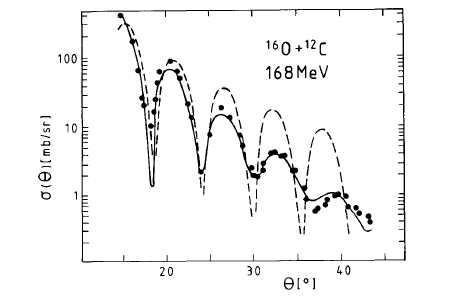
\includegraphics[width=0.4\linewidth]{figs/Fraunhoffer}
	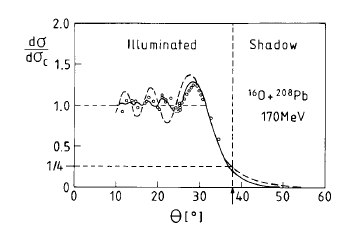
\includegraphics[width=0.4\linewidth]{figs/Fresnel_example}
	\caption{Fraunhoffer /Fresnel diffraction }
	\label{fig:fraunhoffer}
\end{figure}

Fraunhofer diffraction can be obtained in sharp-cutoff strong absorption model with approximation $\eta\simeq 0$.
\bea 
\frac{d\sigma^{FH}}{d\Omega}(\theta)=|i R\frac{J_1(kR\theta)}{\theta}|^2
\eea 

On the other hand, Fresnel diffraction can be obtained in smooth-cutoff strong absorption model
in $\eta\simeq 1$: ratio to Rutherford  to be zero at $\theta>>\theta_{gr}$,
to be 1 at $\theta=0$, to be $1/4$ at grazing angle $\theta=\theta_{gr}$.  
In SAM, $S(l)$ is parameterized with parameters $\lambda_{gr}$ , $\Delta$, $\mu$. 
\bea 
S_l^N = S^N(\lambda) = (1+i\mu \frac{d}{d\lambda}) \frac{1}{1+\exp(\frac{\lambda_{gr}-\lambda}{\Delta})}
\eea 
\begin{figure}[h]
	\centering
	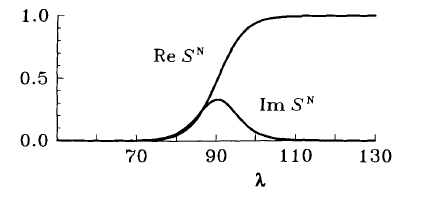
\includegraphics[width=0.4\linewidth]{figs/strong_absorption_model}
	\caption{Strong absorption model is similar to black sphere but with smooth-cutoff
	         as a function $S(l)$ which is absorption below grazing angular momentum
	         is not perfect but still strong. This form can explain Fresnel diffraction pattern.  }
	\label{fig:strongabsorptionmodel}
\end{figure}

\chapter{Coupled Channel equations} 

\section{Terms} 
Let us first make sure the terms to be used.
\begin{itemize}
	\item {\bf Partition} is specified by the projectile and target charge and mass. 
	\item {\bf Excited State pair} or {\bf physical channels} are defined by projectile and 
	      target spin, parity and excitation energy in addition to partition. 
	\item {\bf channels} or {\bf basis} are defined by orbital angular momentum and 
	      total angular momentum of the system in addition to physical channels.       
\end{itemize}

Usually, we consider scattering of plane wave of projectile and target. 
The incident wave function can be considered as
\bea 
\Psi_\vk(\vr, \xi_p,\xi_t) = e^{i\vk\cdot\vr}\phi_p(\xi_p)\phi_t(\xi_t).
\eea 
In case of pure Coulomb scattering we may consider this wave function as
\bea 
\Psi_\vk(\vr, \xi_p,\xi_t) &=& \psi_c(\vk,\vr) \phi_p(\xi_p)\phi_t(\xi_t).
\eea 
with 
\bea 
\psi_c(\vk,\vr)&\sim& e^{-\pi\eta/2}\Gamma(1+i\eta)e^{i\vk\cdot\vr}{}_1F_1(-i\eta,1,i(kr-\vk\cdot\vr))\no 
               &=& e^{i[kz+\eta\ln(k(r-z))]} +f_c(\theta)\frac{e^{i[kr-\eta\ln(2k r)]} }{r} \no 
               &=& \sum_{L} (2L+1) i^L e^{i\sigma_L(\eta)}\frac{F_L(\eta,\rho)}{\rho} P_L(\cos\theta) \no 
               &=& 4\pi \sum_{LM}  i^L e^{i\sigma_L(\eta)}\frac{F_L(\eta,\rho)}{\rho} Y_{LM}(\hat{r})Y_{LM}^*(\hat{k})
\eea 

But, in case of multi-channel scattering, we have to consider all possible channels. 
Because the total angular momentum and parity will be conserved even after reaction, 
it would be convenient to combine spherical harmonics and projectile and target wave functions 
to define channel basis. 

There are several ways to define basis with $L$, $I_p$, $I_t$ and $J_{tot}$. 
By introducing additional $J_p$ or $S$,
\bea 
|\alpha\ra &=& \left[ \left[i^{L} Y_{L}(\hat{R}_x)\otimes \phi^{xp}_{I_p}(\xi_p)\right]_{J_p} 
\otimes \phi^{xt}_{I_t}(\xi_t)\right]_{J_{tot}M_{tot}}, \mbox{ or }\no 
  &=& \left[ \left[ Y_{L}(\hat{R}_x)\otimes \phi^{xp}_{I_p}(\xi_p)\right]_{J_p} 
\otimes \phi^{xt}_{I_t}(\xi_t)\right]_{J_{tot}M_{tot}}, \mbox{ or }\no 
  &=& \left[ i^{L} Y_{L}(\hat{R}_x)\otimes 
                           \left[\phi^{xp}_{I_p}(\xi_p)\otimes \phi^{xt}_{I_t}(\xi_t)\right]_{S}\right]_{J_{tot}M_{tot}}, 
                           \mbox{ or } \no 
 &=& \left[ Y_{L}(\hat{R}_x)\otimes  \left[\phi^{xp}_{I_p}(\xi_p)\otimes \phi^{xt}_{I_t}(\xi_t)\right]_{S}\right]_{J_{tot}M_{tot}}, 
\mbox{ or }.                            
\eea  
From now on, to denote whether $i^L$ factor is included in the definition of $|\alpha\ra$,
let us denote $|i^\alpha,\alpha\ra$ or $|\alpha\ra$. 

From the previous expansion we would expect, the scattering with nuclear potential to be 
\bea 
\Psi_\vk^{(+)}(\vr\xi_p\xi_t)
=\sum_{\alpha_i} \frac{\psi^{(+)}_{\alpha_i}(\vr,\xi_p,\xi_t)}{r} A_{\alpha_i}(\vk)  
\eea 
where 
\bea 
A_{\alpha_i}(\vk) = \frac{4\pi}{k_i} \sum_{M} e^{i\sigma_{L_i}} Y^*_{LM}(\hat{k}) \la \alpha_i|\vk, I_p, I_t\ra 
\eea 
and $\la \alpha_i|\vk, I_p, I_t\ra$ denote all combination of C.G. coefficients and coupling coefficients
to make channel $\alpha_i$. 
The wave function should be expanded in channel basis,
\bea  
\frac{\psi^{(+)}_{\alpha_i}(\vr,\xi_p,\xi_t)}{r}=\sum_{\alpha} |i^\alpha  \alpha\ra \frac{ u_{\alpha,(\alpha_i)}(r)}{r}
\eea 
In this convention, the $i^L$ factor of plane wave limit is included in the channel basis. 
But if one use $|\alpha\ra$ basis, we may define
\bea  
\frac{\psi^{(+)}_{\alpha_i}(\vr,\xi_p,\xi_t)}{r}=\sum_{\alpha} |\alpha\ra \frac{ u_{\alpha,(\alpha_i)}(r)}{r}
\eea 
\bea 
A_{\alpha_i}(\vk) = \frac{4\pi}{k_i} \sum_{M}  i^{L_i} e^{i\sigma_{L_i}} Y^*_{LM}(\hat{k}) \la \alpha_i|\vk, I_p, I_t\ra 
\eea 

The asymptotic form of wave function $u_{\alpha,(\alpha_i)}$ defines scattering or collision matrix.
\bea 
u_{\alpha,(\alpha_i)} \to \frac{i}{2}(I_{\alpha_i}\delta_{\alpha\alpha_i}- S_{\alpha,\alpha_i} O_{\alpha}) 
\eea 
or 
\bea 
u_{\alpha,(\alpha_i)} \to \sqrt{\frac{v_i}{v_\alpha}}\frac{i}{2}(I_{\alpha_i}\delta_{\alpha\alpha_i}
                           - \tilde{S}_{\alpha,\alpha_i} O_{\alpha}) 
\eea 

The asymptotic form becomes
\bea 
\frac{1}{r} \frac{i}{2}\left(H_{L'}^{(-)}\delta_{\alpha'\alpha}-S_{\alpha'\alpha} H_{L'}^{(+)}\right) 
&\to & \frac{1}{r} \sin\Theta_{L}\delta_{\alpha'\alpha} 
+   \frac{e^{i\Theta_{L'}}}{r} \frac{(S_{\alpha'\alpha}-\delta_{\alpha'\alpha})}{2i},   
\eea  
where 
\bea 
\Theta_L=k R- \frac{L\pi}{2}+\sigma_{L}-\eta \ln 2 k R. 
\eea 
The first term becomes original Coulomb function which gives Coulomb scattering amplitude $f_C(\theta)$.
the second term becomes 
\bea 
\frac{e^{i(\rho-\eta \ln 2\rho)}}{r} e^{i\sigma_{L'}} i^{-L'} \frac{(S_{\alpha'\alpha}-\delta_{\alpha'\alpha})}{2i}   
\eea 
Combining this expression for full wave function,
\bea 
\Psi_\vk^{(+)}(\vr,\xi_p,\xi_t)= \psi_c(\vk,\xi_p,\xi_t) 
      +\sum_{\alpha} |i^\alpha \alpha \ra \frac{e^{i(\rho-\eta \ln 2\rho)}}{r} 
        \sum_{\alpha_i} A_{\alpha_i}(\vk)  e^{i\sigma_{L'}} i^{-L'} \frac{(S_{\alpha'\alpha}-\delta_{\alpha'\alpha})}{2i}   
\eea 


This implies the scattering amplitude $f(\theta)$ becomes in the first convention,
multiplying $\phi_{I_p} \phi_{I_t}$ and integrate over internal degrees, 
\bea 
f(\theta)=4\pi\sum_{\alpha_,\alpha} e^{i\sigma_L+i\sigma_{L'}} \frac{(S_{\alpha'\alpha}-\delta_{\alpha'\alpha})}{2ik_i} Y_{L'}(\hat{R})Y_{L}^*(\hat{p}) \la \alpha_i|\vk, I_p, I_t\ra \la I'_p,I'_t|\alpha\ra 
\eea  
where $i^{-L}$ factor cancels with $i^L$ factor in the channel basis. On the other hand, 
the other convention gives 
\bea 
f(\theta)=4\pi\sum_{L,L'} e^{i\sigma_L+i\sigma_{L'}} i^{L-L'}\frac{(S_{\alpha'\alpha}-\delta_{\alpha'\alpha})}{2ik_i} 
Y_{L'}(\hat{R}) Y_{L}^*(\hat{p}) \la \alpha_i|\vk, I_p, I_t\ra \la I'_p,I'_t|\alpha\ra 
\eea  

The differential cross section can be obtained by 
\bea 
\frac{d\sigma_{fi}}{d\Omega}= \frac{v_f}{v_i}|f_c(\theta)\delta_{fi}+f_{fi}(\theta) |^2
\eea 

This gives for unpolarized elastic scattering ( $v_i=v_f$)
\bea 
\frac{d\sigma_{el}}{d\Omega}=\frac{1}{(2I_1+1)(2I_2+1)}\sum_{M_1 M_2}\sum_{M'_1 M'_2}
      | f_C(\Omega)\delta_{M'_1 M_1}\delta_{M'_2 M_2}+ f^{(c M_1 M_2)}_{c M'_1 M'_2}(\Omega)|^2
\eea 
And Inelastic or reaction cross section $\tilde{f}_{fi}=f_c\delta_{fi}+\sqrt{\frac{v_f}{v_i}}f_{fi}$
\bea 
\frac{d\sigma_{c\to c'}}{d\Omega}=\frac{1}{(2I_1+1)(2I_2+1)}\sum_{M_1 M_2}\sum_{M'_1 M'_2}
| f^{(c M_1 M_2)}_{c' M'_1 M'_2}(\Omega)|^2
\eea 








The summation can be analytically done for reaction (Unpolarized cross section의 경우에만 ) as
(Elastic scattering의 경우는 위의 식을 사용하는 것이 좋다.)
\bea 
\frac{d\sigma_{c\to c'}}{d\Omega}=\frac{\pi}{k^2}
 \frac{1}{(2I_1+1)(2I_2+1)}\sum_{\lambda} B_\lambda(E) P_\lambda(\cos\theta)
\eea 
where anisotropy coefficient (즉, Legendre polynomial coefficient) are given by 
\bea 
B_\lambda(E)&=&\frac{1}{4\pi}\sum_{J\pi}\sum_{Il L}\sum_{J'\pi'}\sum_{I' l' L'}
     (-1)^{I-I'} e^{i(\sigma_{l}+\sigma_{l'}-\sigma_L-\sigma_{L'})}
     Z(lJLJ',I\lambda) Z(l'JL'J',I'\lambda)
     S^{J\pi}_{c' I' l',cI l}(E)S^{J'\pi' *}_{c' I' L',cI L}(E)
\eea 
real coefficient Z is defined as
\bea 
Z(lJLJ',I\lambda)&=& (-1)^{J+J'}[(2\lambda+1)(2J+1)(2J'+1)(2l+1)(2L+1)]^{1/2}
 \threejsymbol{l}{L}{\lambda}{0}{0}{0}\sixjsymbol{l}{L}{\lambda}{J'}{J}{I}
\eea 
(which have symmetry  $Z(lJ LJ',I\lambda)=Z(L J' l J,I\lambda)$. Different convention may have
different symmetry and definition of Z. )
Then, integrated cross section or reaction cross section is
\bea 
\sigma_{c\to c'}=\frac{\pi}{k^2}\frac{1}{(2I_1+1)(2I_2+1)}\sum_{J\pi} 
                  (2J+1)\sum_{Il}\sum_{I'l'}| S^{J\pi}_{c' I' l',c I l}(E)|^2 
\eea 

\subsection{In one convention} 
Let us consider the cross section in (L,S) coupling scheme.
Also, convention using $\tilde{S}$-matrix. 
Instead of computing scattering amplitude directly, it is better to compute 
$A^{L'}_{m',M',m,M}$ first because $A^{L'}_{m',M',m,M}$ is independent of angle. 

The FRESCO manual writes  (this is a Condon-Shortley phase convention)
\bea 
Y_{lm}(\theta,\phi)&=& \sqrt{\frac{(2L+1)}{4\pi}\frac{(L-m)!}{(L+m)!}}{\color{red}(-1)^m} e^{im\phi} P_{lm}(cos\theta).
\eea 
However, in Varsharlovich book  Spherical Harmonics are defined without $(-1)^m$ factor. 
In fact, this $(-1)^m$ factor can be absorbed into the phase convention of $P_{lm}(\cos\theta)$
(In case of sci-py package, there is no $(-1)^m$ factor in the expression, however, 
it is included in the definition of Legendre polynomial. Thus, it is consistent with Condon-Shortley convention.)
Thus, one can use either convention. However, one have to make sure about the phase convention 
of associated Legendre polynomial. 

In any case, one can express spherical harmonics as
\bea 
Y_{lm}(\theta,\phi=0)&=& Y_c(l,m) P_{l|m|}(cos\theta)\no 
 Y_c(l,m)&=&\sqrt{\frac{(2L+1)}{4\pi}\frac{(L-|m|)!}{(L+|m|)!}}{\color{red}(-1)^m} \quad \mbox{for } m> 0,\no 
         &=&\sqrt{\frac{(2L+1)}{4\pi}\frac{(L-|m|)!}{(L+|m|)!}} \quad \mbox{for } m<0.
\eea  
(Note that $(-1)^m$ factor will be moved to $m<0$ case in other convention.)

Then, we can express, the scattering amplitude for polarization.
\bea 
\tilde{f}_{m',M'; m, M}(\theta)=\delta_{xx'}\delta_{I_p,I'_p}\delta_{I_t,I'_t} f_c(\theta)
                       +\sum_{L'} \tilde{A}^{L'}_{m' M';m M}\times P_{L'}^{|m'+M'-m-M|}(\cos\theta)   
\eea 
and differential cross section 
\bea 
\frac{d\sigma(\theta)}{d\Omega} =\frac{1}{(2 I_p+1)(2I_t+1)}\sum_{m' M' m M} |\tilde{f}_{m' M':mM}(\theta)|^2
\eea 


The expression 
\bea 
\tilde{A}^{L'}_{m' M';m M}
&=& \sum 
\eea 

\section{Model space wave function}
Because the total angular momentum is a conserved quantity,
one only have to consider coupled channels which having the same total angular momentum.
\bea 
|\Psi^J\ra =\sum_\alpha |\phi_\alpha\ra \psi_\alpha(R_\alpha)
\eea 
where $\alpha$ includes quantum numbers of partitions,
$|\alpha\ra\equiv |x p t; (L I_p)J_p ,I_t; J_{tot} M_{tot}\ra $
where $(x p t)$ represents partition of projectile and target, $L$ is a orbital angular momentum 
between projectile and target, $I_p$ is a spin of projectile, ${\bm J}_p={\bm L}+{\bm I}_p$,
$I_t$ is a spin of target, $J_{tot} M_{tot}$ is a total angular momentum of system and its projection
and $R_\alpha$ is a coordinates between projectile and target.

In other words, more explicit form of $|\phi_\alpha\ra$ is
\footnote{This expression follows the convention in Thompson's textbook.}    
\bea 
|\phi_\alpha\ra &=&  \left[ \left[i^{L} Y_{L}(\hat{R}_x)\otimes \phi^{xp}_{I_p}(\xi_p)\right]_{J_p} 
\otimes \phi^{xt}_{I_t}(\xi_t)\right]_{J_{tot}M_{tot}},
\eea 
where $\phi^{xp}_{I_p}(\xi_p)$ and $\phi^{xt}_{I_t}(\xi_t)$ are bound state wave functions of 
projectile and target with $\xi_p$ and $\xi_t$ as internal coordinates of projectile and target.


\begin{itemize} 
	\item For a system with specific total angular momentum, wave function becomes
	\bea 
	\Psi_{x,J_{tot}}^{M_{tot}}(\vR_x,\xi_p,\xi_t)
	&=&\sum_{\alpha} \left[ 
	\left[i^{L} Y_{L}(\hat{R}_x)\otimes \phi^{xp}_{I_p}(\xi_p)\right]_{J_p} 
	\otimes \phi^{xt}_{I_t}(\xi_t)\right]_{J_{tot}M_{tot}}
	\frac{1}{R_x}f_{\alpha}^{J_{tot}}(R_x) \no 
	&=&\sum_{\alpha} |xpt:(L I_p) J_p,I_t;J_{tot} M_{tot}\ra 
	\frac{f_{\alpha}^{J_{tot}}(R_x) }{R_x} \no 
	&=&\sum_{\alpha} |\alpha; J_{tot} M_{tot}\ra \frac{f_{\alpha}^{J_{tot}}(R_x) }{R_x}
	\eea 
	where $\alpha=(x,p,t,L,I_p,J_p,I_t)$.
	
	\item For a wave function from initial plane wave with momentum $\vk_i$ and spin projections of
	$\mu_{p_i}$ and $\mu_{t_i}$ can be written as 
	\bea 
	\Psi_{x_ip_it_i}^{\mu_{p_i}\mu_{t_i}}(R_x,\xi_p,\xi_t; \vk_i)
	=\sum_{J_{tot}M_{tot}}\sum_{\alpha \alpha_i}
	|\alpha;J_{tot}M_{tot}\ra 
	\frac{f^{J_{tot}}_{\alpha \alpha_i}(R_x)  }{R_x} 
	A^{J_{tot} M_{tot}}_{\mu_{p_i}\mu_{t_i}}(\alpha_i,\vk_i)
	\eea  
	where, "incoming coefficient" is defined as
	\bea 
	A^{J_{tot} M_{tot}}_{\mu_{p_i}\mu_{t_i}}(\alpha_i,\vk_i)
	=\frac{4\pi}{k_i}\sum_{M_i m_i} Y^*_{L_iM_i}(\vk_i)
	\la L_iM_i,I_{p_i} \mu_{p_i}| J_{p_i} m_i\ra 
	\la J_{p_i} m_i,I_{t_i}\mu_{t_i}|J_{tot} M_{tot}\ra. 
	\eea  
	with asymptotic normalization is 
	\bea 
	f_{\alpha\alpha_i}(R_x)\to 
	\frac{i}{2}[H_\alpha^{(-)}(\eta_\alpha,k_\alpha R_\alpha)\delta_{\alpha\alpha_i}
	-S_{\alpha\alpha_i}(k_\alpha) H_\alpha^{(+)}(\eta_\alpha,k_\alpha R_\alpha)]
	\eea 
	
\end{itemize}

where $H^{\pm}$ are Coulomb Hankel functions.

\section{Coupled channel equations}

Let us consider a model space wave function $|\Psi^J\ra$ which have definite 
total angular momentum. Then, coupled channel equation is only for those 
channels having the same total angular momentum. 

One can group full Hamiltonian as
\bea
H= H_{xt}({\bm \xi}_t)+H_{xp}({\bm \xi}_p)+\hat{T}_x({\bm R}_x)+{\cal V}_{xtp}({\bm R}_x,{\bm \xi}_t,{\bm \xi}_p).
\eea 
where 
\bea 
H_{xp}({\bm \xi}_p) \phi^{xp}_{I_p}({\bm \xi}_p)&=&\epsilon_{xp}\phi_{I_p}^{xp}({\bm \xi}_p),\no 
H_{xt}({\bm \xi}_t) \phi^{xt}_{I_t}({\bm \xi}_t)&=&\epsilon_{xt}\phi_{I_t}^{xt}({\bm \xi}_t),
\eea 
relative kinetic term and interaction between target and projectile becomes 
\bea 
\hat{T}_x({\bm R}_x)&=&-\frac{\hbar^2}{2\mu_x}\nabla_{R_x}^2,\no 
{\cal V}_{xtp}({\bm R}_x,{\bm \xi}_t,{\bm \xi}_p)&=&\sum_{i\in p, j\in t} V_{ij}(\vr_i-\vr_j).
\eea 
with reduced mass $\mu_x=\frac{m_{xp}m_{xt}}{m_{xp}+m_{xt}}$.

Assume the Model space Wave function $\Psi$ satisfies,
\bea 
0&=&[{\cal H}-E]|\Psi\ra 
=[{\cal H}-E]|\phi_i\ra \psi_i +
[{\cal H}-E]\sum_{j\neq i}|\phi_j\ra \psi_j
\eea 
If we multiply $\la \phi_i|$ on the left hand side, for each channel $i$, 
\bea 
\la \phi_i|E-{\cal H}|\phi_i\ra \psi_i
= -\sum_{j\neq i}\la \phi_i|E-{\cal H}|\phi_j\ra \psi_j.
\eea 
In the left hand side, it would be natural to express $E-{\cal H}$ in channel $i$,
\bea 
\la \phi_i|E-{\cal H}|\phi_i\ra \psi_i
&=&\la \phi_i|[E-H_i^{bd}-T_i-V_i]|\phi_i\ra \psi_i
=\la \phi_i|[E_i-T_i-V_i]|\phi_i\ra \psi_i \no 
&=&(E_i-T_i(R_i)-\la\phi_i|V_i|\phi_i\ra(R_i))\psi_i(R_i)
\eea 
where $H_i^{bd}$ represent the Hamiltonian which gives projectile and target bound states
in channel $i$,
$V_i={\cal V}_{xtp}({\bm R}_x,{\bm \xi}_t,{\bm \xi}_p)$ is a potential between 
projectile and target in channel $i$, and thus
$\la\phi_i|V_i|\phi_i\ra(R_i)$ implies integration over projectile and target bound state internal coordinates $\xi_p,\xi_t$,
which results in the function with only $R_i$ radial dependence. 
(Note that the channel $|\phi_i\ra$  also contains the orbital angular momentum $\hat{R}_i$ dependence.)

Thus, the equation becomes
\bea
\boxed{  
\left(E_i- T_i(R_i)-U_i\right)\psi_i(R_i) = \la \phi_i|{\cal V}_i-U_i|\phi_i\ra \psi_i(R_i)
                               -\sum_{j\neq i} \la \phi_i|E-{\cal H}|\phi_j\ra \psi_j(R_j) 
                            }
\eea 
where we introduced auxiliary optical potential $U_i$ for channel $i$. 


For the right-hand side, we may use two different ways, in post form
\bea
-\la \phi_i|E-{\cal H}|\phi_j\ra \psi_j
&=& \la \phi_i|T_i-E_i+V_i|\phi_j\ra \psi_j 
= (T_i-E_i) \la \phi_i|\phi_j\ra\psi_j
+\la \phi_i|V_i|\phi_j\ra \psi_j  
\eea 
or in prior form
\bea 
-\la \phi_i|E-{\cal H}|\phi_j\ra \psi_j
&=& \la \phi_i|T_j-E_j+V_j|\phi_j\ra \psi_j 
=  \la \phi_i|\phi_j\ra (T_j-E_j)\psi_j
+\la \phi_i|V_j|\phi_j\ra \psi_j  
\eea 

For the same partition, $x'=x$, we may normalize 
$\hat{N}_{\alpha'\alpha}=\la \phi_{\alpha'}|\phi_{\alpha}\ra=\delta_{\alpha'\alpha}$.
However, in general $\la \phi_i|\phi_j\ra$ are non-orthogonal and may not commute with  $(T_i-E_i)$.

Thus, we get 
\bea 
(E_i-T_i(R_i)-\la\phi_i|V_i|\phi_i\ra(R_i))\psi_i(R_i)
&=&\sum_{j\neq i}\left[ (T_i-E_i) \la \phi_i|\phi_j\ra\psi_j
+\la \phi_i|V_i|\phi_j\ra \psi_j \right] ,\no 
\eea 
or 
\bea 
(E_i-T_i(R_i)-\la\phi_i|V_i|\phi_i\ra(R_i))\psi_i(R_i)
&=&\sum_{j\neq i} \left[ \la \phi_i|\phi_j\ra (T_j-E_j)\psi_j
+\la \phi_i|V_j|\phi_j\ra \psi_j\right]       
\eea 

If we introduce auxiliary optical potential $U_i$, we may rearrange in "post form"
\bea 
(E_i-T_i-U_i)\psi_i
&=& \left( \sum_{j\neq i} \la \phi_i|V_i|\phi_j\ra \psi_j \right)
+\left( [\la\phi_i|V_i|\phi_i\ra-U_i]\psi_i \right) \no & &
+\left( \sum_{j\neq i}  (T_j-E_j)\la \phi_i|\phi_j\ra \psi_j \right)
\eea 
Or, in "prior form",
\bea     
(E_i-T_i-U_i)\psi_i
&=& \left( \sum_{j\neq i} \la \phi_i|V_j|\phi_j\ra \psi_j \right)
+\left( [\la\phi_i|V_i|\phi_i\ra(R_i)-U_i]\psi_i \right) 
\no & & 
+\left( \sum_{j\neq i}  \la \phi_i|\phi_j\ra  (T_j-E_j)\psi_j \right) ,\no   
\eea 
Let us denote 
\bea 
V^{prior}(R_i,R_j)&=&\la \phi_i|V_j|\phi_j\ra,\quad 
V^{post}(R_i,R_j)=\la \phi_i|V_i|\phi_j\ra,
\eea 
If we define $U_i(R_i)=\la \phi_i|V_i|\phi_i\ra$, 
diagonal term in the right hand side would vanish. 

For radial wave function $\psi_\alpha=f_\alpha/R$ in a prior form for rearrangement, 
while separating inelastic scattering and rearrangements counplings,
\footnote{Compared to the coupled channel equation given in FRESCO document,
	(1) we have additional non-orthogonal terms (2) diagonal term in the right side can be
	ignored if $U_x(R_x)\equiv \la \phi_\alpha|{\cal V}_\alpha|\phi_\alpha\ra $
	(3) We have not expanded in multipole of couplings yet (4) $i^{L-L'}$ factor 
	are hidden in the definition of $|\phi_\alpha\ra$. 	
	
}   
\bea 
& &(E_{xpt}-T_{xL}(R_x)-U_x(R_x))f_\alpha(R_x) \no 
& &\quad =\la \phi_\alpha| V_x-U_x|\phi_\alpha\ra(R_x) f_\alpha(R_x) 
+\left( \sum_{\alpha'\neq \alpha} V_{\alpha \alpha'}(R_x)f_{\alpha'}(R_x)\right) 
\no 
& &\quad  +\left(\sum_{x\neq x',\alpha' }\int dR_{x'}  V^{prior}_{\alpha\alpha'}(R_x,R_{x'})
f_{\alpha'}(R_{x'})\right) 
\no & &\quad               
+\left( \sum_{\alpha\neq \alpha'}\int dR_{x'} N_{\alpha\alpha'}(T_{x'L'}-E_{x'p't'})f_{\alpha'}(R_{x'})\right)    
\eea 
where
\bea 
T_{xL}(R)&=&-\frac{\hbar^2}{2\mu_x}\left( \frac{d^2}{dR^2}-\frac{L(L+1)}{R^2}\right),\no 
V_{\alpha\alpha'}(R_x)&=&\la \phi_\alpha|V_x(R_x,\xi)|\phi_{\alpha'}\ra ,\no 
V^{prior}_{\alpha\alpha'}(R_x,R_{x'})&=& R_{x}
\la \phi_\alpha|V^{prior}(R_{x'},\xi)|\phi_{\alpha'}\ra\frac{1}{R_{x'}},\no 
N_{\alpha\alpha'}(R_x,R_{x'})&=& R_x\la \phi_\alpha|\phi_{\alpha'}\ra \frac{1}{R_{x'}}.                     
\eea 

The actual form of couplings requires explicit form of potentials in a certain model.
For example, inelastic channel coupling which have the same partition, 
\bea 
V_{\alpha\alpha'}(R_x)=\int d\xi_p d\xi_t \la i^{L} [Y_L(\hat{R}_x)\otimes \phi_p(\xi_p)]\phi_t(\xi_t)|
V_x(R_x,\xi_p,\xi_t)|i^{L'} 
[Y_{L'}(\hat{R}_{x})\otimes \phi_{p'}(\xi_{p'})]\phi_{t'}(\xi_{t'})\ra 
\eea 
can be described as an collective model or single particle excitation models
for the integration over internal coordinates. 

Also, one may further multipole expand the couplings in terms of transferred angular momentums,
$\Delta L,\Delta S,\Delta J$. 

In the next chapter, let us consider more details on how to obtain couplings 
in various models.

\chapter{Couplings, Interactions}

\section{Multipole expansion of interaction}
In general, the reaction occurs through the interaction between target and projectile,
\bea 
{\cal V}_{xtp}({\bm R}_x,{\bm \xi}_t,{\bm \xi}_p)=\sum_{i\in p, j\in t} V_{ij}(\vr_i-\vr_j)
  ={\cal V}_{xtp}({\bm R}'_x,{\bm \xi}'_t,{\bm \xi}'_p).
\eea 
where if there is a partition change, the interaction can be 
writen either prior or post form. 

In coupled reaction channel calculation, we need to compute (if there is no rearrangement)
couplings 
\bea 
V^{prior}_{\alpha\alpha'}(R_x,R_{x'})&=& R_{x}
\la \phi_\alpha|V^{prior}({\bm R}_{x'},\xi_p,\xi_t)|\phi_{\alpha'}\ra\frac{1}{R_{x'}}. 
\eea 
where integration over internal coordinates and angular integration of ${\bm R}_x$
is implied. (Note that there are $\hat{R}_x$ and $\hat{R}_{x'}$ dependence are
hidden in $|\alpha\ra$ and $|\alpha'\ra$).  

By factoring out factor $i^{L-L'}$, we can write 
\bea 
V^{prior}_{\alpha\alpha'}(R_x,R_{x'})&=&
\int d\Omega_{R_x'} d\xi_p d\xi_t 
\left \la [Y_L(\hat{R}_x)\otimes \phi_p(\xi_p)]_{J_p}\otimes \phi_t(\xi_t)\right| 
 \no & & \times 
R_{x} V_x({\bm R}_{x'},\xi_p,\xi_t)\frac{1}{R_{x'}}\left| 
[Y_{L'}(\hat{R}_{x'})\otimes \phi_{p'}(\xi_{p'})]\otimes \phi_{t'}(\xi_{t'})\right\ra 
\eea 

Let us first do not consider rearrangements. 
\bea 
V_{\alpha\alpha'}(R_x)&=&
\int d^2\Omega_{R_x} d^{3A_p-3}\xi_p d^{3A_t-3}\xi_t 
\left \la [Y_L(\hat{R}_x)\otimes \phi_p(\xi_p)]_{J_p}\otimes \phi_t(\xi_t)\right| 
\no & & \times 
 V_x({\bm R}_{x},\xi_p,\xi_t)\left| 
[Y_{L'}(\hat{R}_{x})\otimes \phi_{p'}(\xi_{p})]\otimes \phi_{t'}(\xi_{t})\right\ra 
\eea 
where
\bea 
{\cal V}_{x}({\bm R}_x,{\bm \xi}_t,{\bm \xi}_p)
&=&\sum_{i\in p, j\in t} V_{ij}(\vr_i-\vr_j) \no 
&=&\sum_{i\in p, j\in t} V_{ij}(\vR_x+{\bm \xi}_{p,i}-{\bm\xi}_{t,j};{\bm s}_i,{\bm s}_j,{\bm t}_i,{\bm t}_j) \no 
&=&\int d{\bm r}_t d{\bm r}_p   
\sum_{i\in p, j\in t} v({\bm R}+\vr_p-\vr_t;{\bm s}_i,{\bm s}_j,{\bm t}_i,{\bm t}_j) 
    \delta^{(3)}(\vr_p-\vr_i)\delta^{(3)}(\vr_t-\vr_j) 
\eea 


By tensor decompose of the potential, we may write\footnote{I suppose
	one would have $T_{\lambda -\mu}(R,{\bm \xi}_t,{\bm \xi}_p)$ in general,
	instead of  $V_\lambda(R)T_{\lambda -\mu}({\bm \xi}_t,{\bm \xi}_p)$.
}
\bea 
{\cal V}_{xtp}({\bm R}_x,{\bm \xi}_t,{\bm \xi}_p)
=\sqrt{4\pi} \sum_{\lambda\mu} V_\lambda(R) Y_{\lambda\mu}(\hat{R}) T_{\lambda -\mu}({\bm \xi}_t,{\bm \xi}_p)
\eea 
Then, the matrix elements for states $\la \alpha'|$ and $|\alpha\ra$
can be expressed in terms of the product of form factor and reduced matrix elements
, $V_\lambda(R)\la \alpha||T_{\lambda}({\bm \xi}_t,{\bm \xi}_p)||\alpha'\ra $, and 
other all coefficients related with shuffling states and tensor decomposition of  
potential. 





In FRESCO, 
the potential operators are decomposed into multipoles and the matrix elements related with
orbital angular momentums are computed by FRESCO so that one only have to give inputs for 
reduced matrix elements and form factors of the coupling $V_\lambda(R)\la \alpha||T_{\lambda}({\bm \xi}_t,{\bm \xi}_p)||\alpha'\ra $. In some special model, even the reduced matrix elements or
form factors will be computed automatically.   

This is explained in the manual of FRESCO and the textbook of I.J. Thompson.
However, there is some convention difference between two. 

\section{Double folding model}
Suppose we have a scalar folding potential $v(\vr_i-\vr_j)$, and full interaction between
projectile and target becomes\footnote{We assumed simple separation of wave function 
	into projectile, target and orbital while ignoring anti-symmetrization of full wave function
	of the system.
} 
\bea 
{\cal V}_{xtp}({\bm R}_x,{\bm \xi}_t,{\bm \xi}_p)&=&\sum_{i\in p, j\in t} v({\bm R}+\vr_i-\vr_j) \no 
&=& \int d{\bm r}_t d{\bm r}_p   v({\bm R}+\vr_p-\vr_t) 
\sum_{i\in p, j\in t} \delta^{(3)}(\vr_p-\vr_i)\delta^{(3)}(\vr_t-\vr_j)     .
\eea 
We can decompose the channel state as 
\bea 
\left| [Y_{L'}(\hat{R}_{x})\otimes \phi_{p'}(\xi_{p'})]\otimes \phi_{t'}(\xi_{t'})\right\ra
= \sum_{M} C_{\alpha,M} Y_{L'}(\hat{R}) \phi_{I_p}(\xi_p)\phi_{I_t}(\xi_t)
\eea 
where $C_{\alpha,M}$ is a collection of Wigner coefficients with projections $M=\{L_z,I_{pz},I_{tz}, J_z\}$.
If we only consider initial and final states as separate product $|Y_{L m}\ra\times |I_p M_p\ra \times |I_t M_t\ra$,
we can simply set $C_{\alpha,M}=1$.
Then,
\bea 
V_{\alpha,\alpha'}(R)&=& \la \alpha| {\cal V}_{xtp}({\bm R}_x,{\bm \xi}_t,{\bm \xi}_p)|\alpha'\ra \no 
&=& \sum_{M,M'} C_{\alpha,M}C_{\alpha',M'} 
\int d{\bm r}_t d{\bm r}_p   \la Y_{Lm}(\hat{R})| v({\bm R}+\vr_p-\vr_t) |Y_{L'm'}(\hat{R})\ra
\no & &  \quad \times  
\la \phi_{I_p,I_{pz} }|\sum_{i}  \delta^{(3)}(\vr_p-\vr_i) |\phi_{I'_p I'_{pz}}\ra 
\la \phi_{I_t,I_{tz}}|\sum_{j}  \delta^{(3)}(\vr_t-\vr_j) |\phi_{I'_t I'_{tz}}\ra    
\eea 
Note that the integration over $\vr_i$ and $\vr_j$ is implied in the matrix element.
For elastic and in-elastic excitation, the number of nucleon does not change in 
initial and final states. 

{\bf However, this expression does not take into account anti-symmetrization of full wave function.}
Later, we will take into account Pauli principle between projectile and target 
as a exchange potential term approximately. 

\subsection{density matrix} 
Let us define density matrix, 
\bea 
\rho_{I I'}(\vr) \equiv \la \phi_{I I_z}|\sum_{i}  \delta^{(3)}(\vr-\vr_i) |\phi_{I' I'_z}\ra.
\eea 
It will correspond to nucleon density of a nucleus if $I=I'$, or  
to transition density if $I\neq I'$.
For example, in H.F. theory, one have for diagonal density as
\bea
\rho(\vr)\simeq \sum_\alpha |\phi_\alpha(r)|^2 
\eea 
where $\alpha$ are single particle states in Hartree-Fock space.
We may want to multipole expand $\rho_{A'A}(\vr)$ by using  
\bea 
\delta^{(3)}(\vr_1-\vr_1)=\frac{\delta(r_1-r_2)}{r_1r_2}\sum_{lm} Y_{lm}(\hat{r}_1)Y^*_{lm}(\hat{r}_2)
\eea 
\bea 
\rho_{A',A}(\vr) &=& \la I_{A'} M_{A'}| \sum_i \delta^{(3)}(\vr-\vr_i)| I_A M_A\ra \no 
    &=& \sum_{L m}  Y^*_{Lm}(\hat{r})\frac{\la I_{A'} M_{A'}|I_A M_A L m\ra}{\sqrt{2 I_{A'}+1} }
      \la A' || \sum_i r_i^{-2}\delta(r-r_i) Y_L(\hat{r}_i)|| A \ra \no 
    &=& \sum_{L m} Y^*_{Lm}(\hat{r}) \la I_{A'} M_{A'}|I_A M_A L m\ra C_L \rho_{A'A,L}(r) . 
\eea 
where we used the Wigner-Eckart theorem and defined multipole of density $\rho_L(r)$.
($\sqrt{2I+1}$ factor depends on the convention of reduced matrix element. )
In other words, 
\bea 
C_L \rho_{A'A,L}(r) = \left(\frac{1}{\sqrt{2 I_{A'}+1} }\right) 
                      \la A'|| \sum_{i} r_i^{-2}\delta(r-r_i) Y_{L}(\hat{r}_i)|| A\ra 
\eea 
where normalization constant $C_L$ is to be chosen for convenience. 
This transition density may be obtained microscopically by computing 
the matrix elements with wave function of $A'$ and $A$. 
On the other hand, one may use macroscopic model by deforming ground state density. 
\footnote{
It is not clear how one can connect the deformation of a spherical density $\rho_0(r)$
for diagonal ground state, to the microscopic definition of a transition density. 
Just formally, if $\rho(\vr)$ is already known and if it is expanded, we should be able to 
define $\rho_{lm}(r)$, 
\bea 
\rho(\vr)=\sum_{lm}  \rho_{lm}(r) Y_{lm}(\hat{r})
\eea 
} 

\subsection{Double Folding using Fourier Transformation}

Let us consider Fourier transformation,
\bea 
\tilde{f}(\vk) =\int d^3 r e^{i\vk\cdot\vr} f(\vr),\quad 
f(\vr) = \int \frac{d^3 \vk}{(2\pi)^3} e^{-i\vk\cdot\vr}\tilde{f}(\vk).
\eea 
We may consider partial wave expansion
\bea 
f(\vr) = \sum_{LM} C_L f_{L}(r) Y_{LM}(\hat{r})
\eea 
where $f_L(r)$ can be written as a integral of $f(\vr)$ with spherical harmonics. 
To use spherical symmetric case as $f(r)=f_0(r)$, 
it is convenient to define $C_{L=0}=\sqrt{4\pi}$, $C_{L\neq 0}=1$. 
Then, the partial wave expansion gives 
\bea 
\tilde{f}(\vk) &=& \int d^3 r \left(\sum_{lm} 4\pi j_l(kr) i^l Y_{lm}(\hat{k}) Y^*_{lm}(\hat{r})        \right) \left( \sum_{l' m'} C_{l'} f_{l'}(r) Y_{l'm'}(\hat{r})  \right) \no 
 &=& \sum_{LM} C_L \tilde{f}_L(k) {\color{red} i^L} Y_{LM}(\hat{k})
\eea 
with 
\bea 
\tilde{f}_L(k)\equiv \int dr (4\pi r^2) j_L(kr)   f_L(r)
\eea 
The inverse relation becomes 
\bea 
f(\vr) &=& \sum_{LM} C_L f_L(r) Y_{LM}(\hat{r})           
\eea 
with 
\bea 
f_L(r)&=&\int \frac{dk k^2}{(2\pi)^3} (4\pi)  j_L(kr) \tilde{f}_L(k)
\eea 
($i^{\pm L}$ factor cancels each other. )

In terms of transition densities, Fourier transformation of density can be written as 
(Note that the complex conjugation of spherical harmonics and factor $i^{\pm L}$ ,
depends on convention.)
\bea 
\rho_{A'A}(\vr)&=&\sum_{L m} \la I_{A'} M_{A'}|I_A M_A L m\ra  Y^*_{Lm}(\hat{r}) C_L \rho_L(r) \no 
\tilde{\rho}_{A' A}(\pm\vk)&=&\sum_{L m} \la I_{A'} M_{A'}|I_A M_A L m\ra i^{\mp L} C_L \tilde{\rho}_L (k) Y^*_{Lm}(\hat{k})
\eea 
with 
\bea 
\tilde{\rho}_L(k) &=& 4\pi \int_0^\infty r^2 dr j_L(kr) \rho_L(r). \no 
\rho_L(r) &=& \int \frac{d k k^2}{(2\pi)^3} (4\pi) j_L(kr) \tilde{\rho}_L(k).
\eea 

We may use Fourier transformation for $v(\vr)$, to simplify multi-dimensional
integrals into series of 1-d integrals,  
\bea 
V_{\alpha,\alpha'}(R)&=&\sum_{M,M'} C_{\alpha,M}C_{\alpha',M'} 
\int d{\bm r}_t d{\bm r}_p \la Y_{L'}(\hat{R})| v({\bm R}+\vr_p-\vr_t) |Y_L(\hat{R})\ra
\rho_{I_p I'_p}(\vr_p)\rho_{I_t I'_t}(\vr_t) \no 
&=& \sum_{M,M'} C_{\alpha,M}C_{\alpha',M'} \int d{\bm r}_t d{\bm r}_p
\int \frac{d^3 k}{(2\pi)^{3}} \la Y_{L'}(\hat{R})| \tilde{v}(\vk) e^{-i\vk\cdot(\vR+\vr_p-\vr_t) } |Y_L(\hat{R})\ra \rho_{I_p I'_p}(\vr_p)\rho_{I_t I'_t}(\vr_t) \no 
&=&  \sum_{M,M'} C_{\alpha,M}C_{\alpha',M'}
\int  \frac{d^3 k}{(2\pi)^{3}} \la Y_{L'}(\hat{R})|  e^{-i\vk\cdot \vR } |Y_L(\hat{R})\ra \times 
\tilde{v}(\vk) \tilde{\rho}_{I_p I'_p}(\vk)\tilde{\rho}_{I_t I'_t}(-\vk)
\eea 

In other words, we may use 
\bea 
U_F(\vR)=\int \frac{d^3 k}{(2\pi)^3} e^{-i\vk\cdot\vR} \tilde{v}(\vk)\tilde{\rho}_1(\vk)\tilde{\rho}_2(-\vk)
\eea 
and
\bea 
\tilde{U}_F(\vk)=\int d^3\vR e^{i\vk\cdot\vR} U_F(\vR) = \tilde{v}(\vk)\tilde{\rho}_1(\vk)\tilde{\rho}_2(-\vk).
\eea   
To get 
\bea 
V_{\alpha,\alpha'}(R) = \sum_{MM'} C_{\alpha,M} C_{\alpha'M'} \la Y_{L'M'}(\hat{R})| U_F(\vR)|Y_{L'M'}(\hat{R})\ra 
\eea 


Then, by the partial wave expansion of plane wave, we get 
\bea 
V_{\alpha,\alpha'}(R)&=& \sum_{\Delta L} \sum_{M,M'}\sum_{L_z}
C_{\alpha,M}C_{\alpha',M'}\la Y_{L'}|  Y_{\Delta L}(\hat{R}) |Y_L\ra
\no & &\times \sqrt{4\pi} i^{-\Delta L}
\int \frac{d^3 k}{(2\pi)^3} j_{\Delta L}(k R)\left( \tilde{v}(\vk) \tilde{\rho}_{I_p I'_p}(-\vk)\tilde{\rho}_{I_t I'_t}(\vk) Y_{\Delta L}^*(\hat{k}) \right) \no 
&=& \sum_{\Delta L} \sum_{M,M'}\sum_{L_z} 
C_{\alpha,M}C_{\alpha',M'}\la Y_{L'}|  Y_{\Delta L}(\hat{R}) |Y_L\ra V_{\alpha,\alpha'}^{\Delta L}(R) 
\eea 
In the last line, we defined a coupling Form factor  $V_{\alpha,\alpha'}^{\Delta L}(R)$
which includes all integration over internal degrees of freedom. 

For scalar interaction $v(|\vr|)$ , 
(direct) folded potential is
\bea 
& & U_F(\vR;A_1\to A'_1,A_2\to A'_2)=\int \frac{d^3 k}{(2\pi)^3} e^{-i\vk\cdot\vR} \tilde{v}(k)\tilde{\rho}_1(\vk)\tilde{\rho}_2(-\vk) \no 
&=&\sum_{LM} i^{-L} Y^*_{LM}(\hat{R})\int \frac{d^3 k}{(2\pi)^3} 4\pi j_L(kR) 
  Y_{LM}(\hat{k}) \tilde{v}(k) \tilde{\rho}_{1}(\vk)\tilde{\rho}_{2}(-\vk) \no 
&=&\sum_{L M,L_1 m_1,L_2 m_2} \la I'_1 M'_1| I_1 M_1 L_1 m_1\ra   \la I'_2 M'_2| I_2 M_2 L_2 m_2\ra
    C_{L_1} C_{L_2} i^{L_1-L_2-L} Y^*_{LM}(\hat{R}) \no 
    & &\times \left( 
    \int \frac{dk k^2 }{2\pi^2} j_L(kR)\tilde{v}(k) \tilde{\rho}_{L_1}(k)\tilde{\rho}_{L_2}(k) \right) \times 
    \left( \int d\Omega_k Y_{LM}(\hat{k})Y^*_{L_1m_1}(\hat{k})Y^*_{L_2 m_2}(\hat{k}) \right) \no 
&=& \sum_{L M,L_1 m_1,L_2 m_2} \la I'_1 M'_1| I_1 M_1 L_1 m_1\ra   \la I'_2 M'_2| I_2 M_2 L_2 m_2\ra
     \la L M| L_1 m_1 L_2 m_2\ra  Y^*_{LM}(\hat{R})\no 
    & &\times  {\color{red} C_{L_1}C_{L_2}\sqrt{\frac{(2L_1+1)(2L_2+1)}{(4\pi)(2L+1)}} i^{L_1-L_2-L}
    	      \la L_1 0 L_2 0| L 0\ra  }
    	      \no & &{\color{red} \times 
    	      \left( 
    	      \int \frac{dk k^2 }{2\pi^2} j_L(kR)\tilde{v}(k) \tilde{\rho}_{L_1}(k)\tilde{\rho}_{L_2}(k) \right) }\no 
&=& \sum_{L M,L_1 m_1,L_2 m_2} \la I'_1 M'_1| I_1 M_1 L_1 m_1\ra   \la I'_2 M'_2| I_2 M_2 L_2 m_2\ra
  \no & &\times 
\la L M| L_1 m_1 L_2 m_2\ra  Y^*_{LM}(\hat{R}) {\color{red} C_L U_{L_1L_2}^L(R) }   	      
\eea 
where multipole of folding potential is defined. 
(One may define $C_{L=0}=(4\pi)^{1/2}$ , $C_{L\neq 0}=1$ for convenience
so that scalar potential is the same as $L=0$ component, $U(R)=U_0(R)$.
This is not the same with Clensch-Goran factors $C_{\alpha,m}$ defined earlier.)
Thus,
\bea 
U^{L}_{L_1,L_2}(R) &=&\int \frac{dk k^2 }{(2\pi)^3}(4\pi) j_L(kR) \tilde{U}^{L}(k),\no 
\tilde{U}^{L}(k)&=&   
    \frac{ C_{L_1}C_{L_2}}{C_L} \sqrt{\frac{(2L_1+1)(2L_2+1)}{(4\pi)(2L+1)}} i^{L_1-L_2-L}
	\la L_1 0 L_2 0| L 0\ra  \no & &\times 
	\tilde{v}(k) \tilde{\rho}_{L_1}(k)\tilde{\rho}_{L_2}(k)
\eea 

\subsubsection{consistency check}
For $L_1+L_2=L$ is from the moments of potential and density,
\bea 
J_k(f^L)&=&4\pi\int f^L(R) r^{k+2} dr, \no 
R_k(f^L)&=& J_{k+2}(f^L)/J_k(f^L),
\eea 
one can do some consistency check,
\bea 
J_L(U^L)=\la L 0|L_1 0 L_2 0\ra \frac{(2L+1)!!}{(2L_1+1)!!(2L_2+1)!!}\frac{\hat{L}_1 \hat{L}_2}{\hat{L}}\frac{C_{L_1} C_{L_2}}{\sqrt{4\pi} C_L} 
 J_{L_1}(\rho^{L_1}_1)J_{L_2}(\rho^{L_2}_2)J_{0}(V^0)
\eea 
and 
\bea 
R_L(U^L)=(2L+3)\left(\frac{R_{L_1}(\rho_1^{L_1})}{(2L_1+3)}
      +\frac{R_{L_2}(\rho_2^{L_2})}{(2L_2+3)}
      +\frac{R_{0}(V^0)}{3} \right) 
\eea 

\subsection{Spin/Isospin dependent folding potential}
If the folding potential have additional dependence on spin or isospin,
\bea 
v_{12}=v_0(r_{12})+v_1(r_{12})\tau_1\cdot\tau_2+v_2(r_{12})\sigma_1\cdot\sigma_2+\cdots 
\eea  
If the isospin does not change during the process we can simply replace, 
$\tau_1\cdot\tau_2\to \tau_1^z \tau_2^z$ and 
\bea 
\la \phi_{I}|\sum_{i}  \delta^{(3)}(\vr-\vr_i)\tau_i^z |\phi_{I'}\ra
= \rho^p_{II'}(\vr)-\rho^n_{II'}(\vr).
\eea  
In a very special case, $\rho_n=\frac{N}{Z}\rho_p=\frac{N}{A}\rho$, this corresponds to 
\bea 
\la \phi_{I}|\sum_{i}  \delta^{(3)}(\vr-\vr_i)\tau_i^z |\phi_{I'}\ra =\frac{Z-N}{A}\rho(\vr)
\eea 


For spin, we would get vector spin transition density 
\bea 
\la \phi_{I}|\sum_{i}  \delta^{(3)}(\vr-\vr_i){\bm \sigma}_i|\phi_{I'}\ra
={\vec \rho}_{II'}(\vr)
\eea 
For G-T transition, we will get,
\bea 
\la \phi_{I}|\sum_{i}  \delta^{(3)}(\vr-\vr_i){\bm \sigma}_i{\bm \tau}^a_i|\phi_{I'}\ra
={\vec \rho}^a_{II'}(\vr)
\eea 

Considering isospin dependence, ($v_{nn}=v_{pp}=v_0+v_1$ and $v_{np}=v_0-v_1$),
\bea 
V= V_0 +V_1 \tau_1\cdot\tau_2 
\eea 
One have double folding potential
\bea 
U_F = U_0 + U_1 \tau_1\cdot\tau_2 
\eea 

Thus, 
\bea 
U_{F_0}&=&\int d^3\vr_1 \int d^3 \vr_2 (\rho_{P n}(r_1)+\rho_{P p}(r_1)  )
(\rho_{T n}(r_2)+\rho_{T p}(r_2)  ) v_0(r_{12}) ,\no 
U_{F_1}&=&\int d^3\vr_1 \int d^3 \vr_2 (\rho_{P n}(r_1)-\rho_{P p}(r_1)  ) 
(\rho_{T n}(r_2)-\rho_{T p}(r_2)  ) v_1(r_{12}). 
\eea 
Thus, in particular case of $\rho_n = \rho_p\times(N/Z) =\rho\times (N/A)$,
\bea 
U_{F1}&=& \left( \frac{N_T-Z_{T}}{A_T}\right) \left( \frac{N_P-Z_{P}}{A_P}\right)
\int d^3\vr_1 \int d^3 \vr_2 \rho_{P}(r_1)
\rho_{T}(r_2) v_1(r_{12})
\eea 
Also transition Form factor from transition density of projectile becomes
\bea 
F_{0} &=& \int d^3\vr_1 \int d^3 \vr_2 (\delta\rho_{P n}(r_1)+\delta \rho_{P p}(r_1)  )
(\rho_{T n}(r_2)+\rho_{T p}(r_2)  ) v_0(r_{12}) ,\no 
F_1&=&\int d^3\vr_1 \int d^3 \vr_2 (\delta \rho_{P n}(r_1)-\delta \rho_{P p}(r_1)  ) 
(\rho_{T n}(r_2)-\rho_{T p}(r_2)  ) v_1(r_{12}). 
\eea 
These form factors can be used for in-elastic scattering cross section. 

\section{Exchange term of Double folding potential}
Let us consider a general process $a_0+A_0\to a+A$.
Let us re-summarize reaction theory. 

The channel internal wave function is 
\bea 
\Psi_{\alpha}(x_\alpha)\equiv \Psi_{\alpha S M_S}(x_\alpha)
=\sum_{M_a M_A}\la J_a M_a J_A M_A|S M_S\ra \Psi_{J_a M_a}(x_a)\Psi_{J_A M_A}(x_A)
\eea 
Spin-angle part of total channel wave function is 
\bea 
\Phi^{(J M_J)}_{\alpha L S}(\hat{R},x_\alpha)
=\sum_{M_L M_S}\la L M_L S M_S|J M_J\ra i^L Y_{L M_L}(\hat{R}) \Psi_\alpha(x_\alpha)
\eea 
Total scattering wave function is
\bea 
\Psi_{J M_J}(R)=\frac{1}{R}\sum_{\alpha LS} \chi^{(J)}_{\alpha LS}(k_\alpha,R) \Phi^{(J M_J)}_{\alpha L S}(\hat{R},x_\alpha).
\eea 
The CC equation is 
\bea 
& &\left\{
\frac{\hbar^2}{2\mu_\alpha}[\frac{d^2}{dR^2}+k_\alpha^2-\frac{L(L+1)}{R^2} ]
     -\la \alpha(LS)J|V|\alpha(LS)J\ra   
\right\} \chi^{(J)}_{\alpha LS}(k_\alpha,R) \no 
&=&\sum_{\alpha' L' S'\neq \alpha L S} 
\la \alpha(LS)J|V|\alpha'(L'S')J\ra   \chi^{(J)}_{\alpha' L'S'}(k_{\alpha'},R)
\eea 
\bea 
\la \alpha'(L'S')J|V|\alpha(LS)J\ra
&=&\int d\hat{R} d x_a d x_A [ \Phi^{(J M_J)}_{\alpha' L'S'}(\hat{R},x_{\alpha'})   ]^*
        V(R) \Phi^{(J M_J)}_{\alpha LS}(\hat{R},x_{\alpha}) \no 
&=& \sum_{M_L M_{L'} M_S M_{S'}}\la L' M_{L'} S' M_{S'}|J M_J\ra \la L M_{L} S M_{S}|J M_J\ra 
\no & &\times 
    \int d\hat{R} [ i^{L'} Y_{L' M_{L'}}(\hat{R})]^*[ i^{L} Y_{L M_{L}}(\hat{R})]
    \la \alpha'(J_{a'} J_{A'})S' M_{S'}|V(\vR)|\alpha(J_a J_A)S M_S\ra.    \nonumber 
\eea 

Usually assumes diagonal potentials are the same local potential for all channels,
\bea 
\la \alpha(LS) J|V|\alpha(LS)J\ra\simeq \la \alpha_0(L_0 S_0)J|V|\alpha_0(L_0S_0)J\ra 
\eea 
With multipole expansion,
\bea 
V(\vR)=\sum_{\lambda\mu} C_\lambda V_\lambda(R)[ i^\lambda Y_{\lambda\mu}(\hat{R})]^*. 
\eea 
with normalization convention $C_0=\sqrt{4\pi}$ and $C_\lambda=1$ for $\lambda\neq 0$.

\bea 
\la \alpha'(L'S')J|V|\alpha(LS)J\ra 
=\frac{1}{\sqrt{4\pi}}\sum_{\lambda} i^{L'-L-\lambda}(-1)^{J-S}\hat{L}\hat{L'}\hat{S}
 \la L 0 L' 0|\lambda 0\ra W(LL'SS';\lambda J) C_\lambda \la \alpha' S'||V_\lambda(R)||\alpha S\ra 
 \no 
\eea 
where, reduced matrix convention is 
\bea 
\la \alpha'(J_{a'}J_{A'})S' M_{S'}|V_{\lambda \mu}(R)|\alpha(J_a J_A) S M_S\ra 
=\la S M_S \lambda \mu|S' M_{S'}\ra 
  \la \alpha' S'||V_\lambda(R)||\alpha S\ra 
\eea 
The folding model, including {\bf knock-on exchange(the interchange of nucleons i and j that occurs when the dinuclear system is antisymmetrized)}, replace $v_{ij}$ as  
\bea 
V=\sum_{i\in a,j\in A} v_{ij} \to v_{ij}(1-P_{ij})=v_D+v_{EX} P^x_{ij}, 
\eea 
\bea 
v_D=v_{ij}^{(D)}=v_{ij},\quad v_{EX}=v_{ij}^{(EX)}=-v_{ij}P^\sigma_{ij} P^\tau_{ij}
\eea 
Then,
\bea 
& &\la \alpha'(J_{a'}J_{A'})S' M_{S'}|V_{\lambda \mu}(R)|\alpha(J_a J_A) S M_S\ra 
\no 
&=&\sum_{M_{a'} M_{A'} M_a M_A}
 \la J_{a'} M_{a'} J_{A'} M_{A'}|S' M_{S'}\ra \la J_{a} M_{a} J_{A} M_{A}|S M_{S}\ra
 \la \alpha'(a'A')|V|\alpha(a A)\ra 
\eea 
with
\bea 
\la \alpha'(a' A')|V|\alpha(aA)\ra 
&=& \sum_{i\in a, j\in A}\sum_{i'\in a',j'\in A'}
    [\la i'j'|v_D|ij\ra +\la i' j'|v_{EX}|ji\ra ] \no 
&=& V^{(D)}_{a'A',aA}(E_\alpha,\vR)+    V^{(EX)}_{a'A',aA}(E_\alpha,\vR,\vR')
\eea 

In a H.F. picture of the system, in a plane wave approximation 
of the relative motion of each nucleus, 
\bea 
\phi_{i\in A_1}(x_1) &=& \varphi_i(r_1)\exp( i k_1\cdot x_1),\no 
\phi_{i\in A_1}(x_2) &=& \varphi_i(r_1+s)\exp( i k_1\cdot x_2),\no 
\phi_{j\in A_2}(x_1) &=& \varphi_j(r_2-s)\exp( i k_2\cdot x_1),\no 
\phi_{j\in A_2}(x_2) &=& \varphi_j(r_2)\exp( i k_2\cdot x_2) 
\eea 
where $\varphi$ are intrinsic wave function of a nucleus. 
We may approximate all nucleons have the same wave number as 
$k_1=K_1/A_1=m v_1$, $k_2=K_2/A_2=m v_2$.
The relative momentum of two nucleus may be written as
$K= \mu (v_1-v_2) = \frac{\mu}{m} (\frac{K_1}{A_1}-\frac{K_2}{A_2})$ 
Then, define density 
\bea 
\sum_{i\in A_1 ,j\in A'_1}\varphi^*_i(\vx_1)\varphi_j(\vx_2) = \rho_{a'a}(\vx_1,\vx_2) 
\eea
Direct term becomes  
\bea 
\sum_{i' j',ij} \la i' j'|v_D|i j\ra &=& \sum_{i' j',ij}\int \phi^*_{i'}(x_1)\phi^*_{j'}(x_2) v_D(s)\phi_i(x_1)\phi_j(x_2) 
                       d^3 r_a d^3 r_A \no 
   &=& \sum_{i' j',ij}\int  \phi^*_{i'}(x_1) \phi_i(x_1) \phi^*_{j'}(x_2)\phi_j(x_2) v_D(s) 
       d^3 r_a d^3 r_A                 \no 
   &=&\sum_{i' j',ij} \int  \varphi^*_{i'}(r_a) \varphi_i(r_a) 
             \varphi^*_{j'}(r_A)\varphi_j(r_A) v_D(s) d^3 r_a d^3 r_A                  \no 
   &=& \int  \rho_{a'a}(r_a,r_a) 
   \rho_{A' A}(r_A,r_A) v_D(s) d^3 r_a d^3 r_A           
\eea 
Exchange term, 
\bea 
\sum_{i' j',ij} \la i' j'|v_{EX}|j i\ra &=& \sum_{i' j',ij}\int \phi^*_{i'}(x_1)\phi^*_{j'}(x_2) v_{EX}(s)\phi_j(x_1)\phi_i(x_2) 
d^3 r_a d^3 r_A \no 
&=& \sum_{i' j',ij}\int  \phi^*_{i'}(x_1) \phi_i(x_2) \phi^*_{j'}(x_2)\phi_j(x_1) v_{EX}(s) 
d^3 r_a d^3 r_A                 \no 
&=& \sum_{i' j',ij}\int  \varphi^*_{i'}(r_a) \varphi_i(r_a+s) e^{i k_1\cdot(x_2-x_1)}  \varphi^*_{j'}(r_A)\varphi_j(r_A-s)e^{i k_2\cdot(x_1-x_2) }   v_{EX}(s) 
d^3 r_a d^3 r_A \no 
&=& \int \rho_{a' a}(r_a,r_a+s)\rho_{A',A}(r_A,r_A-s) v_{EX}(s) 
         e^{i (k_1-k_2)\cdot(x_2-x_1) }  d^3 r_a d^3 r_A \no 
&=& \int \rho_{a' a}(r_a,r_a+s)\rho_{A',A}(r_A,r_A-s) v_{EX}(s) 
\exp(i \frac{m}{\mu} K \cdot s )  d^3 r_a d^3 r_A           
\eea 
In fact, the relative momentum ${\bm K}(R)$should depends on the distance between nuclei as
\bea 
\frac{K^2(R)}{2\mu} +V(E_\alpha,R)+V_C(R) = E_\alpha
\eea 


The direct term is local if potential is local and can be written as
\bea 
V^{(D)}_{a'A',aA}(E_\alpha,\vR) &=&\int \rho_{a'a}(\vr_a)\rho_{A'A}(\vr_A) v_D(\rho,E_\alpha,s)
      d^3 r_a d^3 r_A, \no 
    {\bm s}&=&\vr_A-\vr_a+\vR 
\eea 
On the other hand , exchange term can be approximated as
\bea 
V^{(EX)}_{a'A',aA}(E_\alpha,R) = \int \rho_{a'a}(\vr_a,\vr_a+{\bm s})
           \rho_{A' A}(\vr_A,\vr_A-{\bm s}) v_{EX}(\rho,E_\alpha,s)
           \exp(\frac{i {\bm K(R)} {\bm s}}{M_\alpha}) d^3 r_a d^3 r_A
\eea 
where $M_{\alpha}= a A/(a+A)$.

One may simplify the problem, by treating only the diagonal radial part of potential 
in a g.s. density for $V(R)$ in $K(R)$. 
Note that $V^{EX}$ have to be calculated as self consistently. 

Let us a bit generalize the F.T. method. 
Define ${\bm x}={\bm r}_a-{\bm r}_A$, ${\bm y}=(\vr_a+\vr_A)/2$
and with change of variables, 
\bea 
& &\int d^3\vr_a d^3 \vr_A f(\vr_a,\vr_A,{\bm s}=\vR+\vr_A-\vr_a,\vR) \no 
&=&\int d^3{\bm x} d^3 {\bm y} f(\vr_a={\bm y}+\frac{{\bm x}}{2},
                               \vr_A={\bm y}-\frac{{\bm x}}{2},{\bm s}=\vR-{\bm x},\vR) ,\no 
&=&\int d^3{\bm s} d^3 {\bm y} f(\vr_a={\bm y}+\frac{{\bm R}}{2}-\frac{{\bm s}}{2},
\vr_A={\bm y}-\frac{{\bm R}}{2}+\frac{\bm s}{2},{\bm s},\vR)                                 
\eea 
In an approximation of density matrix expansion, 
\bea 
& &\rho(\vr,\vr+{\bm s}) \simeq \rho(\vr+{\bm s}/2)\hat{j}_1( {\bm k_F}(\vr+\frac{{\bm s}}{2})\cdot {\bm s}) ,\no 
& &\hat{j}_1(x) = 3(\sin(x)-x\cos(x))/x^3,
\eea 
with position dependent Fermi momentum $k_F(r)$,
\bea 
k_F(r) =\left\{  \left[\frac{3}{2}\pi^2\rho(\vr)   \right]^{3/2}
               +\frac{5 C_S[\nabla \rho(\vr)]^2} {3\rho(\vr)^2}
               +\frac{5\nabla^2\rho(\vr)}{36\rho(\vr)}
         \right\}^{1/2}, \quad C_S=\frac{1}{36}? \frac{1}{4}?
\eea 

Density matrix can be formally written as
\bea 
\rho(\vR+\frac{\bm s}{2},\vR-\frac{\bm s}{2})
&=&\sum_{a} \phi_a^*(\vR+\frac{\bm s}{2})\phi_a(\vR-\frac{\bm s}{2}) \no 
&=& e^{{\bm s}\cdot(\nabla_1-\nabla_2)/2}\sum_a \phi_a^*(\vR_1)\phi_a(\vR_2)|_{\vR_1=\vR_2=\vR}
\eea 
If time-reversed orbitals are filled pairwise,(in other words, $\phi^*_m(x)=\phi_{-m}(x)$) 
linear term vanishes,
\bea 
(\nabla_1-\nabla_2)[\phi_m^*(R_1)\phi_m(R_2)+\phi_m(R_1)\phi_m^*(R_2)]=0.
\eea 
Question: Because of using this property, it is only valid for even-even nucleus(?). 
Then, involving only even powers, angular integral of the square of a density matrix may be 
replaced by the integral of the square of the angle average of the density matrix, 
\bea 
\rho(\vR+\frac{\bm s}{2},\vR-\frac{\bm s}{2})
= F (  (\frac{\nabla_1-\nabla_2}{2})^2)\rho(\vR_1,\vR_2)
\eea 
where
\bea 
F(k^2)=\frac{\sinh(ks)}{ks}, k^2>0,\quad \frac{\sin(ks)}{ks}, k^2<0.
\eea 
F is expanded around some average value $-k^2$, 
\bea 
F (  (\frac{\nabla_1-\nabla_2}{2})^2)
 &=& F(-k^2)+F'(-k^2)\left[ (\frac{\nabla_1-\nabla_2}{2})^2+k^2\right]+\dots \no 
 &=& j_0(ks) +\frac{s}{2k} j_1(ks)\left[ (\frac{\nabla_1-\nabla_2}{2})^2+k^2\right]+\dots
\eea 

we can change the double folding integral into a form of 
\bea 
&\to& \int d^3 s d^3 y f_1(\vr_a+\frac{\bm s}{2}={\bm y}+\frac{\bm R}{2},{\bm s})
    f_2(\vr_A-\frac{\bm s}{2}={\bm y}-\frac{\bm R}{2} ,{\bm s}) 
    v({\bm s})\exp(\frac{i {\bm K(R)} {\bm s}}{M_\alpha}) \no 
&=& \int d^3 s d^3 y\int \frac{d^3 k_1}{(2\pi)^3} \frac{d^3 k_1}{(2\pi)^3}
    e^{-ik_1\cdot(y+\frac{R}{2})}\tilde{f}_1(k_1,s) 
    e^{-ik_2\cdot(y-\frac{R}{2})}\tilde{f}_2(k_2,s) v(s) \exp(\frac{i {\bm K(R)} {\bm s}}{M_\alpha})\no 
&=& \int d^3 s \int \frac{d^3 k}{(2\pi)^3} e^{-ik\cdot R}\tilde{f}_1(k ,s) 
\tilde{f}_2(-k,s) v(s) \exp(\frac{i {\bm K(R)} {\bm s}}{M_\alpha})    \no 
&\to& \int ds s^2 (4\pi) j_0( \frac{K(R)s}{M_\alpha})v(s) 
    \int \frac{dk k^2}{2\pi^2} j_0(k R)\tilde{f}_1(k ,s)\tilde{f}_2(-k,s)
\eea 
By using this property, at least one of the integration can be simplified using F.T. 


\subsection{M3Y potential}
Reference: PHYSICAL REVIEW C 69, 024610 (2004), PHYSICAL REVIEW C 84, 064602 (2011)

In double folding model, actually there can be two different kind of folding, direct term, 
\bea 
U_D(R)= g(E_p)\int d^3 \vr_p \int d^3 \vr_t \rho_{p}(\vr_p) v_D(\vR+\vr_p-\vr_t) \rho_{t}(\vr_t),
\eea
where $g(E_p)$ is a correction for energy dependence 
and exchange term,
\bea 
U_E(R) = g(E_p)\int d^3\vr_p \int d^3\vr_t  \rho_p(\vr_p;\vr_p+{\bm s}) v_E({\bm s})\rho_t(\vr_t;\vr_t-{\bm s})
         exp( i\vk_{rel}\cdot{\bm s} /A_{rel}) 
\eea 
where ${\bm s}=\vR+\vr_p-\vr_t$, $A_{rel}=A_p A_t/(A_p+A_t)$, $k_{rel}^2(R)=2 m_n A_{rel}[E_{cm}-U(R)]/\hbar^2$.
The exchange term is usually approximated as a zero-range $\delta$ function terms. (Dao T. Khoa, W. von Oertzen, and H. G. Bohlen, Phys. Rev. C
49, 1652 (1994).) (The finite range version of exchange term have 3 Yukawa functions.)

The most frequently used nucleon-nucleon potentials in the theory of
nuclear reactions are so-called density-dependant M3Y-Reid and M3Y-Paris
potentials (here M is for Michigan,Y is for Yukawa)(Review: M.E. Brandan, G.R. Satchler, The interaction between light heavy-ions
and what it tells us, Physics Reports 285 (1997) 143-243 ). 
These fitted to reproduce G-matrix calculation. 

In general on the potential can be spin-isospin dependent, $V_{ST}$,
\bea 
v(r) =V_{00}+V_{01}\tau_1\cdot\tau_2 +V_{10}\sigma_1\cdot\sigma_2+V_{11}\tau_1\cdot\tau_2\sigma_1\cdot\sigma_2. 
\eea 

\begin{itemize}
	\item The potential $v(r)$ can be charaterized in terms of its moments
	  \bea 
	  J_v &=& \int dr 4\pi r^2 v(r) ,\no 
	  \la r^2\ra _{v} &=& \left( \int dr 4\pi r^4 v(r) \right) / J_v 
	  \eea 
	  For example, above $M3Y-Reid$ gives $J_{00}=-146$ MeV.fm$^3$ and $\la r^2\ra_v=7.26$ fm$^2$.
	\item Exchange term correction in zero-range approximation for $S=T=0$\footnote{
		There are several different values of exchange term values. One may need to check the reference.
		Some case it is written as $J_{ex}=-262$ for Reid. 
	}
	\bea 
	v_{00}(r)&\to v_{00}(r)+F_{ex}(E) \delta(r) ,\no 
	F_{ex}(E)&\simeq J_{ex}(1-\tau E/A) ,\no 
	\mbox{M3Y-Reid : }&  J_{ex}=-276,\quad \tau=0.005 ,\no 
	\mbox{M3Y-Paris : }&  J_{ex}=-590, \quad \tau=0.002.
	\eea 
	This is not consistent with expression in PHYSICAL REVIEW C 69, 024610 (2004),
	where energy dependence is an overall factor.
	
	
	\item More generally, (according to the PHYSICAL REVIEW C 69, 024610 (2004))
	\bea 
	v_{00,D}(r) &=& \sum_{i=1}^3 G_{D_i} \frac{e^{-\mu_i r}}{\mu_i r},\no  
	v_{00,E}(r) &=& \sum_{i=1}^3 G_{E_i} \frac{e^{-\mu_i r}}{\mu_i r},\quad \mbox{or } G_{E\delta}\delta^3(r)  
	\eea 
	Energy dependence is approximated as
	\bea 
	g(E_p)= 1- k E_p.
	\eea 
	
	\item Parameters of bare M3Y is summarized as
	
	\begin{tabular}{|c|c|c|}
		\hline 
		Coefficients & Reid & Paris \\ 
		\hline 
		$G_{D1}$(MeV) & 7999 & 11062 \\ 
		\hline 
		$G_{D2}$(MeV) & -2134 & -2537.5 \\ 
		\hline 
		$G_{D3}$(MeV) & 0 & 0 \\ 
		\hline 
		$G_{E1}$(MeV) & 4631.4 & -1524.25 \\ 
		\hline 
		$G_{E2}$(MeV) & -1787.1 & -518.75 \\ 
		\hline 
		$G_{E3}$(MeV) & -7.847 & -7.847 \\ 
		\hline 
		$\mu_1$(fm$^{-1}$) & 4 & 4 \\ 
		\hline 
		$\mu_2$ & 2.5 & 2.5 \\ 
		\hline 
		$\mu_3$ & 0.707 & 0.707 \\ 
		\hline 
		$G_{E\delta}$(MeV fm$^3$) & -276 & -592 \\ 
		\hline 
		k(MeV$^-1$) & 0.002 & 0.003 \\ 
		\hline 		
	\end{tabular} 
	
	\item Density dependence: But it is known that {\bf one have to use density dependent NN potential for nuclear matter saturation}.
	Density dependence is introduced as 
	\bea 
	v^{DD}(r;\rho_{FA},E)= f(\rho_{FA},E) v_{NN}(r),
	\eea 
	where
	\bea 
	f(\rho_{FA},E)&=& C(E) \left[ 1+\alpha(E) \exp(-\beta(E) \rho_{FA})-\gamma \rho_{FA} \right],
	\eea  
	where the density is defined in a somewhat arbitrary as
	\bea 
	\rho_{FA} = \rho_{p}(\vr_p)+\rho_t(\vr_t),\mbox{ or } \rho_{p}(\vr_p+{\bm s}/2)+\rho_t(\vr_t-{\bm s}/2).
	\eea 
	This density dependence introduce a little bit of complication in folding potential. 
	\item In DDM3Y, $\gamma=0$. In BDM3Y, $\alpha=0$. CDM3Y is a combination of DDM3Y and BDM3Y. 
	 The parameters are fitted to reproduce correct saturation of nuclear matter. 
     Parameters of DDM3Y are summarized as (different choice gives different nuclear matter incompressibility.)
    
    \begin{tabular}{|c|c|c|c|c|c|}
    	\hline 
    	DD label & interaction & C & $\alpha$ & $\beta$(fm$^{-3}$) & $\gamma$(fm$^{-3}$) \\ 
    	\hline 
    	0 & D independent & 1 & 0 & 0 & 0 \\ 
    	\hline 
    	1 & DDM3Y1-Paris & 0.2963 & 3.7231 & 3.7384 & 0 \\ 
    	\hline 
    	2 & CDM3Y1 & 0.3429 & 3.0232 &  3.5512 &  0.5 \\ 
    	\hline 
    	3 & CDM3Y2 &  0.3346  & 3.0357  & 3.0685 &  1.0 \\ 
    	\hline 
    	4 & CDM3Y3 &  0.2985  & 3.4528  & 2.6388 &  1.5 \\ 
    	\hline 
    	5 & CDM3Y4-Paris &  0.3052  & 3.2998  & 2.3180 &  2.0 \\ 
    	\hline 
    	6 & CDM3Y5 &  0.2728  & 3.7367 &  1.8294 &  3.0 \\ 
    	\hline 
    	7 & CDM3Y6 &  0.2658  & 3.8033 &  1.4099  & 4.0 \\ 
    	\hline 
    	8 & BDM3Y1-Paris &  1.2521 &  0.0 &  0.0  & 1.7452
    	\\ 
    	\hline 
    	9 &DDM3Y-Reid & 0.2845 & 3.6391 & 2.9605 & 0.0 \\
    	\hline 
    	10 & BDM3Y-Reid & 1.2253 & 0.0 & 0.0 & 1.5124 \\
    	\hline 
    \end{tabular} 
    
	\item On the other hand, iso-spin dependent part for Reid potential,
	\bea
	V_{01}(r)= -4886 \frac{e^{-4 r}}{4r}+1176\frac{e^{-2.5r}}{2.5 r}+217\delta^3(r). 
	\eea 

\end{itemize}

The transition density are sometimes approximated as a derivative WS form,
\bea 
\beta_{L}^{(N)} R_{W} \frac{d}{dr} W(R) = \beta_{L}^{(N)}(\frac{W R_W}{a_W})\frac{e^x}{(e^x+1)^2}
\eea 
while, $\beta_2^{(N)}$ may be determined from $\beta_2^{(c)}$ which 
is obtained from $B(E2)$ assuming uniform charge radius $R_c=1.2 A^{1/3}$ fm ,
\bea 
\beta_2^{(N)} R_W = \beta_2^{(c)} R_c
\eea 

\subsection{Folding of DDM3Y}
Here, only elastic part of folding potential will be considered. 
Details can be found in the Appendix of D.T. Khoa and G.R. Satchler, NPA668(2000)3-41. 

Direct and exchange potential is 
\bea 
U_D(R)= \int d^3 \vr_p \int d^3 \vr_t \rho_{p}(\vr_p) v_D(\vR+\vr_p-\vr_t) \rho_{t}(\vr_t),
\eea
\bea 
U_E(R) = \int d^3\vr_p \int d^3\vr_t  \rho_p(\vr_p;\vr_p+{\bm s}) v_E({\bm s})\rho_t(\vr_t;\vr_t-{\bm s}) exp( i\vk_{rel}\cdot{\bm s} /A_{rel}) 
\eea 
with density matrix expansion approximation of transition density. 

Density/Energy dependence of M3Y potential is assumed,
\bea 
C g(E) [1 +\alpha e^{-\beta \rho_{FA}}-\gamma \rho_{FA}] v_{D,E}(s)
\eea 

Direct potential
\bea 
V_0^{(D)}(E,R)&=& \frac{ C g(E)}{2\pi^2}\int_0^\infty \Big[
                     \rho^a_0(k) \rho^A_0(k) +\alpha \bar{\rho}^a_0(k)\bar{\rho}^A_0(k)
                \no & &\quad\quad      
                     -\gamma (\tilde{\rho}^a_0(k)\bar{\rho}^A_0(k)+\bar{\rho}^a_0(k)\tilde{\rho}^A_0(k) )
                   \Big] v_D(k) j_0(k R) k^2 dk   
\eea 
where,
\bea 
v_D(k) &=& 4\pi\int_0^\infty v_D(r) j_0(k r) r^2 dr,\no 
\rho^{a,A}_0(k)&=&4\pi\int_0^\infty \rho^{a,A}_0(r) j_0(k r) r^2 dr ,\no 
\bar{\rho}^{a,A}_0(k)&=&4\pi\int_0^\infty \rho^{a,A}_0(r) e^{-\beta \rho^{a,A}_0(r) }j_0(k r) r^2 dr ,\no 
\tilde{\rho}^{a,A}_0(k)&=&4\pi\int_0^\infty [\rho^{a,A}_0(r)]^2 j_0(k r) r^2 dr
\eea 

Exchange potential 
\bea 
V^{(E)}_0(E,R)&=& 4\pi C g(E)\int_0^\infty G_0(R,s) j_0(K(R)s/M)) v_{EX}(s) s^2 ds,
\eea 
where
\bea 
G_0(R,s)&=&\frac{1}{2\pi^2}\int_0^\infty\Big[ f_a(k,s) f_A(k,s) +\alpha \bar{f}_a(k,s)\bar{f}_A(k,s)
            -\gamma[f_a(k,s) \tilde{f}_A(k,s)+\tilde{f}_A(k,s) f_{A}(k,s) ]   \Big]  
            j_0(kR) k^2 dk 
\eea 
and 
\bea 
f_{a(A)}(k,s)&=&4\pi\int_0^\infty \rho^{a,A}_0(r) \hat{j}_1( k_{F_{a,A}}(r) s) j_0(k r) r^2 dr ,\no 
\bar{f}_{a(A)}(k,s)&=&4\pi\int_0^\infty \rho^{a,A}_0(r) e^{-\beta\rho_{a,A}(r)}
    \hat{j}_1( k_{F_{a,A}}(r) s) j_0(k r) r^2 dr ,\no 
\tilde{f}_{a(A)}(k,s)&=&4\pi\int_0^\infty [\rho^{a,A}_0(r)]^2 \hat{j}_1( k_{F_{a,A}}(r) s) j_0(k r) r^2 dr 
\eea 
\bea 
\frac{\hbar^2 K(R)^2}{2m M} = E_{cm}- V(E,R)-V_C(R)
\eea 
where $E_{cm}$ is a center of mass energy, while $E$ is an incident laboratory energy per nucleon
and $M=\frac{A_1 A_2}{A_1+A_2}$. $V(E,R)=V_D(E,R)+V_E(E,R)$.
\bea 
\hat{j}_1(x)&=& \frac{3(\sin(x)-x\cos(x))}{x^3},\no 
k_{F_{a,A}}(r)&=& \left\{  \left[\frac{3}{2}\pi^2\rho(\vr)   \right]^{3/2}
+\frac{5 C_S[\nabla \rho(\vr)]^2} {3\rho(\vr)^2}
+\frac{5\nabla^2\rho(\vr)}{36\rho(\vr)}
\right\}^{1/2}, \quad C_S=\frac{1}{36}? \frac{1}{4}?
\eea 
\begin{itemize}
	\item From the assumed density dependence, we can write direct term 
	    \bea 
	    U_D(R) = C(E) U_{D1}(R)+C(E)\alpha(E) U_{D\alpha}(R)-C(E)\gamma U_{D\gamma}(R)
	    \eea 
	   and exchange term 
	   \bea 
	   U_{EX}(R) = C(E) U_{EX1}(R)++C(E)\alpha(E) U_{EX\alpha}(R)-C(E)\gamma U_{EX\gamma}(R)
	   \eea 
	\item $U_{D1}$ can be done as previous F.T. method.
	  \bea 
	   U_{D1}(R) &=& \int d^3 \vr_p \int d^3 \vr_t \rho_{p}(\vr_p) v_D({\bm s}) \rho_{t}(\vr_t)
	  \eea 
	  
	  if we are only dealing with spherical density and spherical potential, we need only 
	  spherical bessel transformation with $l=0$. 
	  
	  Only considering $L=0$ components of potential and density, 
	  \bea 
	  U_{D1}(R)=\int \frac{dk k^2}{(2\pi)^3} 4\pi  j_0(k R)\tilde{U}_{D1}(k),
	  \quad \tilde{U}_{D1}(k)= \tilde{v}_D(k) \tilde{\rho}_p(k) \tilde{\rho}_t(k) 
	  \eea 
	  \bea 
	  \tilde{f}_D(k)=4\pi \int d r r^2 j_0(kr) f(r), \quad f=(v,\rho_p,\rho_t)
	  \eea 
	  
	  
	\item For $U_{D\alpha}$, it is convenient to choose  $\rho_{FA} = \rho_{p}(\vr_p)+\rho_t(\vr_t)$,
	  \bea 
	  U_{D\alpha} &=& \int d^3 \vr_p \int d^3 \vr_t 
	  \rho_{p}(\vr_p)e^{-\beta\rho_{p}(\vr_p)} 
	  \rho_{t}(\vr_t)e^{-\beta\rho_{p}(\vr_t)} v({\bm s}). 
	  \eea 
	  This can be done as like previous F.T. method, except that we need 
	  \bea 
	  U_{D\alpha}(R) = \int \frac{dk k^2}{(2\pi)^3} 4\pi  j_0(k R) 
	      v_D(k)\tilde{\rho}_{p,D\alpha}(k) \tilde{\rho}_{t,D\alpha}(k) 
	  \eea 
	  with 
	  \bea 
	   \tilde{\rho}_{D\alpha}(\vk)&\to& 
	      \int d^3\vr e^{-i\vk\cdot\vr} \rho(\vr)e^{-\beta\rho(\vr)},\no 
	      &\to& 4\pi \int dr r^2 j_0(kr) \rho(r)e^{-\beta\rho(r)}
	  \eea 
	  
	  
	\item For $U_{D\gamma}$, it is convenient to choose  $\rho_{FA} = \rho_{p}(\vr_p)+\rho_t(\vr_t)$,
	  \bea 
	   U_{D\gamma}&=& \int d^3 \vr_p \int d^3 \vr_t 
	   \rho_{p}(\vr_p)(\rho_{p}(\vr_p)+\rho_{t}(\vr_t)) 
	   \rho_{t}(\vr_t) v_D({\bm s}) \no 
	   &=&\int \frac{dk k^2}{(2\pi)^3} 4\pi j_0(k R) \left( \tilde{\rho}_p(k)\tilde{\rho}_{t,D\gamma}(k)
	                                                    +\tilde{\rho}_t(k)\tilde{\rho}_{p,D\gamma}(k)  
	                                       \right) \tilde{v}_D(k)             
	  \eea  
	  This also can be done as like previous  F.T. method except that now it have sum of two terms
	  and one $\rho(\vk)$ have to be replaced as
	  \bea 
	  \tilde{\rho}_{D\gamma}(\vk)&\to& 
	  \int d^3\vr e^{-i\vk\cdot\vr} \rho(\vr)^2 ,\no 
	  &\to& 4\pi \int dr r^2 j_0(kr) \rho(r)^2 
	  \eea 
	  
	\item For $U_{EX1}$, it is convenient to choose  $\rho_{FA} = \rho_{p}(\vr_p+{\bm s}/2)+\rho_t(\vr_t-{\bm s}/2)$,
	  \bea 
	   U_{EX1}& \simeq& \int d^3\vr_p \int d^3\vr_t  
	   \rho_p(\vr_p+{\bm s}/2)\hat{j}_1( {\bm k_F}(\vr_p+\frac{{\bm s}}{2})\cdot {\bm s})
	   \rho_t(\vr_t-{\bm s}/2)\hat{j}_1( {\bm k_F}(\vr_t-\frac{{\bm s}}{2})\cdot {\bm s})
	   \no & &\times   v_E({\bm s})  exp( i\vk_{rel}\cdot{\bm s} /A_{rel}) \no 
	   &=& \int d^3{\bm y} \int d^3{\bm s}  
	   \rho_p({\bm y}-\frac{\vR}{2})\hat{j}_1( {\bm k_F}({\bm y}-\frac{\vR}{2})\cdot {\bm s})
	   \rho_t({\bm y}+\frac{\vR}{2})\hat{j}_1( {\bm k_F}({\bm y}+\frac{\vR}{2})\cdot {\bm s})
	   \no & &\times   v_E({\bm s})  exp( i\vk_{rel}\cdot{\bm s} /A_{rel})
	  \eea 
	  Then, consider F.T.
	  \bea 
	  \rho_p({\bm y}-\frac{\vR}{2})\hat{j}_1( {\bm k_F}({\bm y}-\frac{\vR}{2})\cdot {\bm s})
	  = \int \frac{d^3 k}{(2\pi)^3} e^{-i\vk\cdot({\bm y}-\frac{\vR}{2})}
	     \tilde{f}_1({\bm k},{\bm s})
	  \eea 
	  We can obtain 
	  \bea 
	  \tilde{f}(\vk,s)  = 4\pi \int dx x^2 j_0( k x) \rho(x)\hat{j}_1(k_F(x)s ) 
	  \eea 
	  
	  Then, above integral changes into 
	  \bea 
	  U_{EX1}&=& \int d^3{\bm s}\int\frac{d^3 k}{(2\pi)^3}
	                e^{i\vk\cdot\vR} 
	                \tilde{f}_1(\vk,{\bm s})\tilde{f}_2(-\vk,{\bm s})
	                v_E({\bm s}) e^{ i\vk_{rel}\cdot{\bm s} /A_{rel}} \no 
	          &\to& 4\pi \int ds s^2 j_0(\frac{k_{rel}(R) s}{A_{rel}}) v_E(s)
	               \left(\int \frac{dk k^2}{2\pi^2} j_0(k R) \tilde{f}_1(k,s) \tilde{f}_2(k,s)  \right)     
	  \eea 
	  
	  Thus, one needs to compute series of spherical Bessel transformation. 
	  
	\item For $U_{EX\alpha}$, it is convenient to choose  $\rho_{FA} = \rho_{p}(\vr_p+{\bm s}/2)+\rho_t(\vr_t-{\bm s}/2)$,
	  \bea 
	   U_{EX\alpha} &=& \int d^3{\bm s}\int\frac{d^3 k}{(2\pi)^3}
 	                    e^{i\vk\cdot\vR} 
 	                   \tilde{f}_1(\vk,{\bm s})\tilde{f}_2(-\vk,{\bm s})
	                    v_E({\bm s}) e^{ i\vk_{rel}\cdot{\bm s} /A_{rel}} 
	                    \no 
	                    &\to& 4\pi \int ds s^2 j_0(\frac{k_{rel}(R) s}{A_{rel}}) v_E(s)
	                    \left(\int \frac{dk k^2}{2\pi^2} j_0(k R) \tilde{f}_1(k,s) \tilde{f}_2(k,s)  \right)
	  \eea 
	  this time $\tilde{f}_1({\bm k},{\bm s})$ (also $\tilde{f}_2({\bm k},{\bm s})$ similarly)
	  is defined as 
	  \bea 
	   \rho_p({\bm y}-\frac{\vR}{2})e^{-\beta \rho_p({\bm y}-\frac{\vR}{2}) }\hat{j}_1( {\bm k_F}({\bm y}-\frac{\vR}{2})\cdot {\bm s})
	   = \int \frac{d^3 k}{(2\pi)^3} e^{-i\vk\cdot({\bm y}-\frac{\vR}{2})}
	   \tilde{f}_1({\bm k},{\bm s})
	  \eea 
	  This implies
	  \bea 
	  \tilde{f}(\vk,{\bm s}) \to  4\pi \int dx x^2 j_0(k x) \rho(x)e^{-\beta \rho(x)}\hat{j}_1(k_F(x) s)
	  \eea 
	  
	  
	\item For $U_{EX\gamma}$, it is convenient to choose  $\rho_{FA} = \rho_{p}(\vr_p+{\bm s}/2)+\rho_t(\vr_t-{\bm s}/2)$,
	\bea 
	  U_{EX\gamma}(R) &=& 
	     \int d^3{\bm s}\int\frac{d^3 k}{(2\pi)^3} e^{i\vk\cdot\vR} 
	      \left[\tilde{f}^m_1(\vk,{\bm s})\tilde{f}_2(-\vk,{\bm s})+
	      \tilde{f}_1(\vk,{\bm s})\tilde{f}^m_2(-\vk,{\bm s})\right] 
	          v_E({\bm s}) e^{ i\vk_{rel}\cdot{\bm s} /A_{rel}} \no 
	       &\to & 4\pi \int ds s^2 j_0(\frac{k_{rel}(R) s}{A_{rel}}) v_E (s) 
	       \left( \int \frac{dk k^2}{2\pi^2} j_0(k R)
	       (\tilde{f}_p(k,s)\tilde{f}^m_t(k,s)+\tilde{f}^m_p(k,s)\tilde{f}_t(k,s) )  \right)  \no 
	\eea 
	where 
	\bea 
	\rho_p({\bm y}-\frac{\vR}{2})\hat{j}_1( {\bm k_F}({\bm y}-\frac{\vR}{2})\cdot {\bm s})
	&=& \int \frac{d^3 k}{(2\pi)^3} e^{-i\vk\cdot({\bm y}-\frac{\vR}{2})}
	\tilde{f}_1({\bm k},{\bm s}) \no 
	\rho^2_p({\bm y}-\frac{\vR}{2})\hat{j}_1( {\bm k_F}({\bm y}-\frac{\vR}{2})\cdot {\bm s})
	&=& \int \frac{d^3 k}{(2\pi)^3} e^{-i\vk\cdot({\bm y}-\frac{\vR}{2})}
	\tilde{f}^m_1({\bm k},{\bm s})
	\eea 
	In the same way,
	\bea 
	\tilde{f}(k,s) &\to& 4\pi \int dx x^2 j_0(k x) \rho_p(x)\hat{j}_1( {\bm k_F}(x)\cdot {\bm s})  ,\no 
	\tilde{f}^m(k,s) &\to& 4\pi \int dx x^2 j_0(k x) \rho^2_p(x)\hat{j}_1( {\bm k_F}(x)\cdot {\bm s})
	\eea 
\end{itemize}


\subsection{Parametrization of density,potential and F.T.}
There are commonly used forms.
\begin{itemize}
	\item 2-parameter Fermi form (WS form)
	\bea 
	\rho_{2pF}(r)=\rho_0\left[1+\exp\left(\frac{r-R}{a}\right)\right]^{-1}
	\eea 
	here $\rho_0$ is extracted by the constraint of the volume integral 
     \bea 
     4\pi\int dr r^2 \rho(r) =X.
     \eea 
     (This can be approximated as
     \bea 
     \rho_0 = \frac{3 X}{4\pi R^3}\left[1+(\frac{\pi a}{R})^2+6(\frac{a}{R})^3 e^{-R/a}+\dots\right] 
     \eea 
     )
     
	\item 2-parameter Gaussian form
	\bea 
	\rho_{2pG}(r)=\rho_0 \exp\left(-\frac{r^2}{R^2}\right) 
	\eea 
	where normalization 
	\bea 
	\rho_0 = \frac{X}{\pi^{3/2} R^3}
	\eea 
	F.T.
	\bea 
	\tilde{\rho}(k) = \rho_0 \pi^{3/2} R^3 e^{-R^2 k^2/4}
	\eea 
	
	\item 3-parameter Fermi/Gaussian form
	\bea 
	\rho_{3pF}(r)=\left[1+\omega \frac{r^2}{R^2}\right]\rho_{2pF}(r)  
	\eea 
	
	\item Delta form 
	\bea 
	V_0 \delta^{(3)}(\vr)
	\eea 
	F.T. 
	\bea 
	\tilde{V}(k) = V_0.
	\eea 
	
	\item Yukawa form (and pure Coulomb)
	\bea 
	V(r)=V_0\frac{e^{-\mu r}}{\mu r}
	\eea 
	F.T. 
	\bea 
	\tilde{V}(k)= \frac{4\pi V_0}{\mu}\frac{1}{k^2+\mu^2}
	\eea 
	\item 
	One global parametrization is available from Sao Paulo potential. 
	They use 2-parameter Fermi function, with $R_0=1.31 A^{1/3}-0.84$ and $a=0.56$ fm. 
	Note that this is for matter distribution of Sao-Paulo folding potential. 
	(In other words, it is not a point nucleon distribution. ) 
	For point nucleon distribution, $R_{0C}=1.76 Z^{1/3}-0.96$, $R_{0p}=1.81 Z^{1/3}-1.12$, $R_{0n}=1.49 N^{1/3}-0.79$. 
	with $a=0.5$ fm. 
	
\end{itemize}


\section{Sao-Paulo potential}
In Sao-Paulo potential, nuclear density is parameterized as
\bea 
R_p &=& 1.81 Z^{1/3}-1.12,\quad a_p = 0.47-0.00083 Z,\no 
R_n &=& 1.49 N^{1/3}-0.79,\quad a_n = 0.47+0.00046 N
\eea  
Alternatively, 
or 
\bea 
R_{M} &=& 1.31 A^{1/3}-0.84,\quad a_M = 0.56 
\eea  
 
Then, the local equivalent(LE) SP potential in zero-range approach\footnote{There is a non-local version too.}
 is  
\bea 
V_{SP}(R,E) &=& V_F(R) \exp(- 4 v^2/c^2), \no 
v^2(R,E) &=& \frac{2}{\mu}[E-V_C(R)-V_{SP}(R,E)]
\eea 
where velocity $v^2(R,E)$ should be obtained in a self consistent way. 
While, the energy independent folding potential part is 
\bea 
V_F(R) = \int \rho_1(r_1)\rho_2(r_2) V_0\delta^{(3)}(R-r_1+r_2) d^3 r_1 d^3 r_2, 
\quad V_0 = -456\ \mbox{MeV.fm}^3
\eea 

 
\section{DWBA matrix element}
In DWBA approximation, initial and final state wave function becomes 
distorted waves and only potential for transition is included in the matrix element. 
\bea 
T^{DWBA}={}^{(-)}\la \vk_f; I_{p_f} M_{p_f} I_{t_f} M_{t_f}|V_{fi}|\vk_i;I_{p_i} M_{p_i} I_{t_i} M_{t_i}\ra^{(+)} 
\eea 
where $V_{fi}$ depends on the reaction and convention. 

In partial wave form,
\bea 
T^{DW}_{\alpha\alpha_i}&=&
{}^{(-),DW}\la k_\alpha, \alpha \phi_\alpha | V_\beta | k_{\alpha_i}, \alpha_i \phi_{\alpha_i}\ra^{(+),DW},\no 
| k_{\alpha}, \alpha,\phi_\alpha\ra^{(\pm),DW}
&=&\left[ \left[i^{L_\alpha} Y_{L_\alpha}(\hat{R}_\alpha)
           \otimes \phi_{I_p,\alpha}(\xi_{p,\alpha})\right]_{J_p}
           \otimes \phi_{I_t,\alpha}(\xi_{t,\alpha})         
            \right]_{J_\alpha M_\alpha}  \frac{\chi_{\alpha}^{(\pm),DW}(R_{\alpha})}{R_{\alpha}}.
\eea 
If there is no rearrangement(inelastic scattering), 
the potential $V_\beta(R_\alpha,\xi_p,\xi_t)$ and relative wave functions are
all function of $R_\alpha$. Thus, integral is over 
\bea 
\int d^3 R_\alpha d^{3(p-1)}\xi_p d^{3(t-1)}\xi_t
\eea 

In case of rearrangement, the initial DW is described in $R_i$
but final DW is described in $R_f$. Thus, there should be relation(or Jacobian)
connecting coordinates $(R_i,\xi_{p,i},\xi_{t,i})$ 
and $(R_f,\xi_{p,f},\xi_{t,f})$.
\bea 
\int d^3 R_i d^{3(p-1)}\xi_{p_i} d^{3(t-1)}\xi_{t_i}
=J \int d R_i \int d R_f  
  (\int \mbox{ integral over internal degrees })(R_i,R_f)
\eea 
The exact integration depends on the particular assumption on the 
structure model of bound nuclei and transition mechanism. 

In other words, for reaction $a(=b+x)+A\to b+B(=A+x)$, integration is either
\bea 
d^3 \vR_\alpha d^3 \vr_x [d^3 \xi_b]_{b-1}[d^3\xi_A]_{A-1} 
\eea 
or 
\bea 
d^3 \vR_\beta d^3 \vr_x [d^3 \xi_b]_{b-1}[d^3\xi_A]_{A-1}. 
\eea 
We can convert $d^3\vr_x\to (factor) d^3 R_\beta$ in the first choice
or $d^3\vr_x\to (factor) d^3 R_{\alpha}$ for the second choice
by using the relation between coordinates. 


For example, in the figure, we can change $r_1$ as a function of $R_a$. 
Then, 
\bea 
\vr_1&=&\frac{m_B m_a}{m_x(m_a+m_A)}(\vr_a-\frac{m_b}{m_a}\vr_b), 
\eea 
and thus, we get
\bea 
d\vr_b d\vr_1= J d\vr_b d\vr_a,\quad J=\left(\frac{m_B m_a}{m_x(m_a+m_A)}\right)^3
\eea 
Or, equivalently,
\bea 
\vr_2&=& \frac{m_A m_a}{m_x(m_a+m_A)}(\vr_a-\frac{m_B}{m_A}\vr_b),
\eea 
\bea 
d\vr_a d\vr_2 = J' d\vr_a d\vr_b,\quad J' =\left( \frac{m_B m_a}{m_x(m_a+m_A)}\right)^3  
\eea 

For example, if there is no target spin dependent interaction in the optical potential
\footnote{
Usually, spin-orbit interaction is related with the projectile spin.
} , there is no target spin projection change in distorted wave(but, projectile spin projection
can change), 
\bea 
T^{DWBA}&=&{}^{(-)}\la \vk_f; I_f M_f s_f \sigma_f|V_{fi}|\vk_i;I_i M_i s_i \sigma_i\ra^{(+)} \no 
&=&J \sum_{\sigma'_i\sigma'_f} \int d {\bm R}_f \int d{\bm R}_i
     \chi^{(-),*}_{\sigma'_f \sigma_f}(\vk_f,{\bm R}_f)
     \la I_f M_f s_f \sigma'_f|V_{fi}|I_i M_i s_i \sigma'_i\ra({\bm R}_f,{\bm R}_i)
     \chi^{(+)}_{\sigma'_i \sigma_i}(\vk_i,{\bm R}_i)  \no 
\eea 
where, $\la I_f M_f s_f \sigma'_f|V_{fi}|I_f M_f s_f \sigma'_f\ra({\bm R}_f,{\bm R}_i)$
implies integration over all internal coordinates with bound state wave functions. 
The spin index summation over $\sigma'$ are introduced for the case that 
the distorting potential is spin-dependent. 
And Jacobi factor is from converting natural coordinate system into ${\bm R}_i$ and ${\bm R}_f$.
In case of post form, natural integral variable is ${\bm R}_f$ and ${\bm r}_f$.
(In prior form, they are ${\bm R}_i$ and ${\bm r}_i$). Thus, Jacobi factor is to 
change ${\bm r}_f$ into ${\bm R}_i$.

The potential for transfer reaction in DWBA is
\bea 
V_{fi} &=& V_{xA}(\vr_1) +V_{bA}(\vR) -U_{aA}(\vR_\alpha) ,\quad \mbox{in prior form}\no  
       &=& V_{xb}(\vr_2) +V_{bA}(\vR) -U_{bB}(\vR_\beta),\quad \mbox{in post form}   
\eea 
where $\vr_1$, $\vr_2$ and $\vR$ are function of $\vR_\alpha$ and $\vR_\beta$.
In zero-range approximation or neglecting remnant correction, 
the second and third terms for transfer reaction are ignored. 

\begin{figure}
\centering
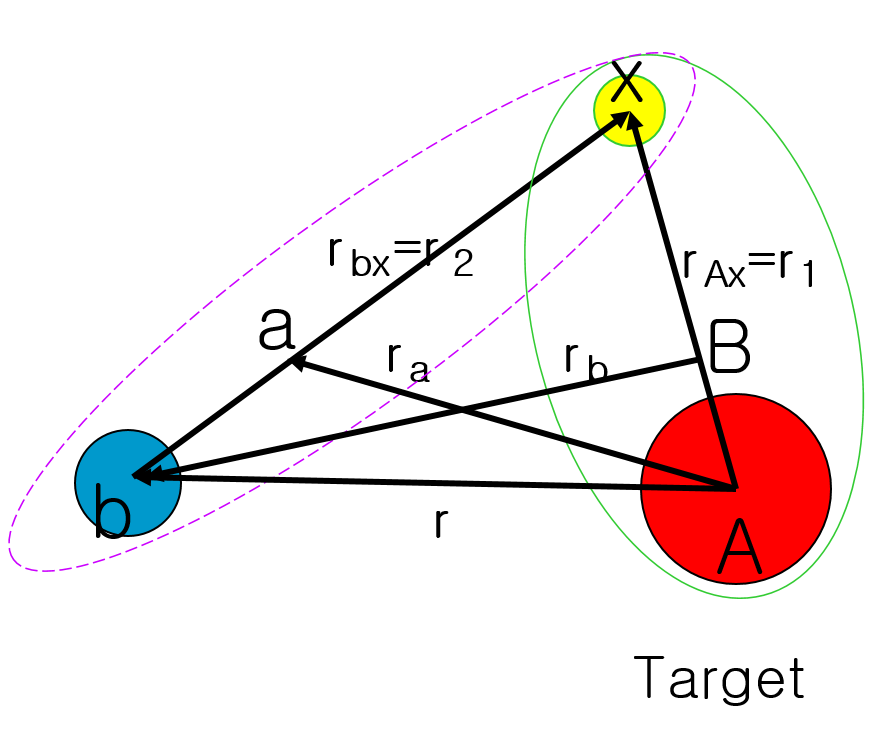
\includegraphics[width=0.5\linewidth]{stripping}
\caption{
	Direction of arrow are chosen so that from heavier to lighter particle.
	$\vR_\alpha = \vr_1-\frac{m_b}{m_b+m_X}\vr_2$, $\vR_\beta=\frac{m_A}{m_A+m_x}\vr_1-\vr_2$. 
         $\vR=\vr_1-\vr_2=\frac{m_a \vR_\alpha+m_B \vR_\beta}{m_a+m_A}$ .   }
\label{fig:stripping}
\end{figure}
Suppose projectile stripping such that projectile $a=b+x$ stripped and
bound state $B=A+x$ is formed(See Figure).
In the post representation, natural coordinate will be $R_b$ and $r_1$. 



And, distorted wave is expanded in partial waves
\bea 
\chi^{(+)}_{m'm}(\vk,\vr)&=& \frac{4\pi}{k r}
  \sum_{JLM} \la L M, sm| J,M+m\ra \la L M+m-m',s m'|J M+m\ra 
    i^L \chi^{(+)}_{LJ}(kr) Y_{LM}^*(\hat{k}) Y_{L,M+m-m'}(\hat{r}),\no 
\chi^{(+)}_{LJ}(kr)&\to& \frac{i}{2}\exp(i\sigma_L) [H_L^{(-)}(kr)-\eta^J_L H_L^{(+)}(kr)]    
\eea 
, $\eta^J_L$ is a reflection coefficient or S-matrix. (주의: 여기서는 Coulomb phase factor를 
distorted partial wave 에 포함 시켰음.)

Since the Hamiltonian is a scalar, we can write 
\bea 
\Delta J=I_i-I_f=L_f-L_i+s_f-s_i=\Delta L +\Delta s
\eea 
and $V$ can be multipole expanded in ranks of $\Delta J,\Delta L, \Delta s$. 

Thus, the most important information we need to compute is 
$\la I_f M_f s_f \sigma'_f|V_{fi}|I_f M_f s_f \sigma'_f\ra({\bm R}_f,{\bm R}_i)$
which is also a central part of coupled channel calculation. 
Details of computing this kernel will be discussed in next chapter. 

If we ignore internal structures of $b$ and $A$, only projectile and target 
s.p. wave function of x in projectile and target appears in the matrix elements
$\la I_f M_f s_f \sigma'_f|V_{fi}|I_f M_f s_f \sigma'_f\ra({\bm R}_f,{\bm R}_i)$.
In other words, after partial wav expansion,
\bea 
I(\vr_1,\vr_2) &=& \la I_f M_f s_f \sigma'_f|V_{fi}|I_f M_f s_f \sigma'_f\ra({\bm R}_f,{\bm R}_i),\no 
 &=& \sum C^{(1)}_{I_B I_A j l_1 n_1 I_x a_x} C^{(2)}_{s_a s_b s l_2 n_2 I_x a_x}
          \no & &\times  
           (I_A M_A j m_j|I_B M_B)(s_b m_b s m_s|s_a m_a)
          (l_1 m_1 I_x M_x|j m_j)(l_2 m_2 I_x M_x|s m_s)
          \no & &\times 
          \phi_{l_1 m_1 n_1}(\vr_1) W(\vr_2) \phi_{l_2 m_2 n_2}(\vr_2)    
\eea 
in post form with ${\bm I}_B-{\bm I}_A={\bm j}$, ${\bm s}_b-{\bm s}_a={\bm s}$, ${\bm s}+{\bm j}={\bm l}$ and $C^{(1,2)}$ are c.f.p
in target and projectile bound states.  

\section{Coupled equation sets}
모든 가능한 channel을 고려하는 것은 불가능하므로, 적은수의 coupled model space를 생각해야한다.
여기서, model space wave function을 간단히 나타내자.
\bea 
|\Psi\ra =\sum_{\alpha} |\phi_\alpha\ra \psi_\alpha 
\eea 
여기서, channel $\alpha$는 partition과 partial wave 를 모두 포함한 것이고, 
$|\phi_\alpha\ra$ 에는 boudn state와 관련된 모든 양이 포함되고, 
$\psi_\alpha$에는 incoming coefficient를 비롯한 scattering wave의 모든 것이
포함되어 있다고 하자. 말하자면, 
\bea 
|\phi_\alpha\ra &=&  \left[ \left[i^{L} Y_{L}(\hat{R}_x)\otimes \phi^{xp}_{I_p}(\xi_p)\right]_{J_p} 
    \otimes \phi^{xt}_{I_t}(\xi_t)\right]_{J_{tot}M_{tot}},\no 
\psi_\alpha &=& \frac{\chi^{J_{tot}}_{\alpha \alpha_i}(R_x)  }{R_x} 
   \underbrace{A^{J_{tot} M_{tot}}_{\mu_{p_i}\mu_{t_i}}(\alpha_i,\vk_i)},    
\eea 
여기서 $\psi_\alpha$는 아직 분모의 $R$을 빼내기 전이다. 또는 $i^L Y_L(\hat{R}_x)$
까지 $\psi_\alpha$ 에 포함시켜서 생각하면, bound state $|\phi_\alpha\ra$ 는
internal degree of freedom 만 포함하게 된다. Underbrace part는 kinematic part로써,
partial wave decomposition of initial wave function 을 나타낸다. (즉, 
$|\Psi\ra$ 가 plane wave 인 경우 
$|\vk_i,\mu_{p_i},\mu_{t_i}\ra=
\sum_{\alpha_i}|\Psi_{\alpha_i}\ra 
A^{J_{tot} M_{tot}}_{\mu_{p_i}\mu_{t_i}}(\alpha_i,\vk_i)$ 로 분해된다. 만약 $|\Psi\ra$ 가 
이미 잘 정의된 total angular momentum을 가지는 경우에는 이 부분은 필요가 
없다. 아래식에서는 사실상 $|\Psi_{\alpha_i}\ra$ 으로 생각하자.) 

full Wave function $\Psi$ 는 $[{\cal H}-E]\Psi=0$ 을 만족한다.
원래의 many-body system full Hamiltonian ${\cal H}$은 A-body 에 대한 operator 이지만,
각 channel에 따라 여러가지 다른 방식으로 regroup 할 수 있다. 
\bea
H= H_{xt}({\bm \xi}_t)+H_{xp}({\bm \xi}_p)+\hat{T}_x({\bm R}_x)+{\cal V}_{xtp}({\bm R}_x,{\bm \xi}_t,{\bm \xi}_p).
\eea 
여기서, $H_{t,p}$는 target과 projectile의 bound state를 기술하는 Hamiltonian이고,
\bea 
H_{xp}({\bm \xi}_p) \phi^{xp}_{I_p}({\bm \xi}_p)&=&\epsilon_{xp}\phi_{I_p}^{xp}({\bm xi}_p),\no 
H_{xt}({\bm \xi}_t) \phi^{xt}_{I_t}({\bm \xi}_t)&=&\epsilon_{xt}\phi_{I_t}^{xt}({\bm \xi}_t),
\eea 
relative kinetic term and interaction between target and projectile becomes 
\bea 
\hat{T}_x({\bm R}_x)&=&-\frac{\hbar^2}{2\mu_x}\nabla_{R_x}^2,\no 
{\cal V}_{xtp}({\bm R}_x,{\bm \xi}_t,{\bm \xi}_p)&=&\sum_{i\in p, j\in t} V_{ij}(\vr_i-\vr_j).
\eea 
with reduced mass $\mu_x=\frac{m_{xp}m_{xt}}{m_{xp}+m_{xt}}$.

Let us rewrite the full equation for the scattering wave. 
\bea 
0&=&[{\cal H}-E]|\Psi\ra 
  =[{\cal H}-E]|\phi_i\ra \psi_i +
    [{\cal H}-E]\sum_{j\neq i}|\phi_j\ra \psi_j
\eea 
If we multiply $\la \phi_i|$ on the left hand side, (it is just a separation of terms
and no orthogonality of wave functions are assumed.)
\bea 
\la \phi_i|E-{\cal H}|\phi_i\ra \psi_i
= -\sum_{j\neq i}\la \phi_i|E-{\cal H}|\phi_j\ra \psi_j.
\eea 
The left hand side can be simplified by
\bea 
\la \phi_i|E-{\cal H}|\phi_i\ra \psi_i
&=&\la \phi_i|[E-H_i^{bd}-T_i-V_i]|\phi_i\ra \psi_i
=\la \phi_i|[E_i-T_i-V_i]|\phi_i\ra \psi_i \no 
&=&(E_i-T_i(R_i)-\la\phi_i|V_i|\phi_i\ra(R_i))\psi_i(R_i)
\eea 

여기서, $V_i={\cal V}_{xtp}({\bm R}_x,{\bm \xi}_t,{\bm \xi}_p)$ 이고 ,
$\la\phi_i|V_i|\phi_i\ra(R_i)$는 bound state internal coordinate $\xi_p,\xi_t$
에 대한 적분이 내포된다. 

For the right-hand side, we may use two different ways,
\bea
-\la \phi_i|E-{\cal H}|\phi_j\ra \psi_j
&=& \la \phi_i|T_i-E_i+V_i|\phi_j\ra \psi_j 
   = (T_i-E_i) \la \phi_i|\phi_j\ra\psi_j
     +\la \phi_i|V_i|\phi_j\ra \psi_j  
\eea 
or 
\bea 
-\la \phi_i|E-{\cal H}|\phi_j\ra \psi_j
&=& \la \phi_i|T_j-E_j+V_j|\phi_j\ra \psi_j 
   =  \la \phi_i|\phi_j\ra (T_j-E_j)\psi_j
     +\la \phi_i|V_j|\phi_j\ra \psi_j  
\eea 
같은 partition 안에서는 $x'=x$,
$\hat{N}_{\alpha'\alpha}=\delta_{\alpha'\alpha}$ 으로 normalize 되어 있다고 생각한다.
여기서, $\la \phi_i|\phi_j\ra$ 는 non-orthogonal 이고, rearrangement channel의 경우에는
$R_i$ 또는 $R_j$ 에 대한 함수가 되기 때문에 $(T_i-E_i)$와 commute하지 않을 수 있다. 
정리하면,
\bea 
(E_i-T_i(R_i)-\la\phi_i|V_i|\phi_i\ra(R_i))\psi_i(R_i)
&=&\sum_{j\neq i}\left[ (T_i-E_i) \la \phi_i|\phi_j\ra\psi_j
     +\la \phi_i|V_i|\phi_j\ra \psi_j \right] ,\no 
&=&\sum_{j\neq i} \left[ \la \phi_i|\phi_j\ra (T_j-E_j)\psi_j
     +\la \phi_i|V_j|\phi_j\ra \psi_j\right]       
\eea 

Here, if we introduce auxiliary optical potential $U_i$,
\bea 
(E_i-T_i-U_i)\psi_i
&=& \left( \sum_{j\neq i} \la \phi_i|V_i|\phi_j\ra \psi_j \right)
   +\left( [\la\phi_i|V_i|\phi_i\ra-U_i]\psi_i \right) \no & &
   +\left( \sum_{j\neq i} \la \phi_i|\phi_j\ra (T_j-E_j)\psi_j \right)
\eea 
Or,
\bea     
(E_i-T_i-U_i)\psi_i
&=& \left( \sum_{j\neq i} \la \phi_i|V_j|\phi_j\ra \psi_j \right)
   +\left( [\la\phi_i|V_i|\phi_i\ra(R_i)-U_i]\psi_i \right) 
   \no & & 
   +\left( \sum_{j\neq i}  (T_j-E_j)\la \phi_i|\phi_j\ra \psi_j \right) ,\no   
\eea 
보통의 경우, $\la \phi_i|V_i|\phi\ra\to U_i$ 로 근사시키기 빼문에 오른쪽의 항 하나는 사라지게 된다.
그러나, $U_i$를 auxiliary field로 쓰는 경우 오른쪽 항이 필요하게 된다. 

아직 $1/R$을 분리하지 않았기 때문에, 여기서 $T_i=-\frac{\hbar^2\nabla^2_i}{2\mu_i}$
이다. (Text book 3.2.2. 의 식은 $1/R$을 분리한 다음이다.)
\footnote{
$\sum_{j\neq i}$ part에도 optical potential을 도입하면, 오른쪽항을
\bea 
\sum_j [\la \phi_i| V_j-U_j|\phi_j\ra ]\psi_j 
+\sum_{j\neq i} \la \phi_i|(T_j+U_j-E_j)|\phi_j\ra \psi_j
\eea 
로 쓸 수 있다. 즉, $V_j$ 대신 $W_j=V_j-U_j$를 사용하는 것과 같게 된다. 
} 
이때, $\la \phi_i|\phi_j\ra$ is non-orthogonality terms. And
\bea 
V^{prior}(R_i,R_j)&=&\la \phi_i|V_j|\phi_j\ra,\quad 
V^{post}(R_i,R_j)=\la \phi_i|V_i|\phi_j\ra,
\eea 
If we define $U_i(R_i)=\la \phi_i|V_i|\phi_i\ra$, 
diagonal term in the right hand side would vanish. 

여기까지는 wave function이 각 channel에서 projectile 과 target의 곱이 된다는 것 이외에
어떠한 가정도 이루어 지지 않았다. 그러나, potential matrix element를 
얻기 위해서는 bound state 의 structure에 대한 model이 필요하다. (이것을 
bound state의 form factor라고 부른다.)

따라서, coupled channel equation을 만들기 위해서는 bound state wave function과 
각 component 사이의 interaction 이 주어져야 하고, 이를 바탕으로 potential matrix element
를 계산해야 한다.( 이 때 interaction의 형태도 모델에 따라 달라짐에 주의.) 
이렇게 CC equation이 얻어진 다음에는 이를 풀어서 channel wave function을 
구한다. 

일반적으로, 1차 DWBA를 생각할 때는 non-orthogonality term $\hat{N}_{\alpha\alpha'}$ 
or remnant interaction may be ignored.

다시 쓰면, $p=(post\mbox{ or }prior)$, 
\bea 
(E_i-T_i-U_i)\psi_i=\left( \sum_{j\neq i} V^{p}(R_i,R_j)\psi_j\right) 
                   +\left( \la \phi_i| V_i-U_i|\phi_i\ra \psi_i \right) 
                   +\left( \sum_{j\neq i} K_{ij}(T_j-E_j)\psi_j\right)    
\eea 
한편, $j\neq i$ 중에는 partition이 같은 inelastic channel과 partition이 달라지는 
rearrangement channel이 있다. inelastic channel의 경우에는 하나의 $R_i$만으로 
coupling potential을 나타낼 수 있어 post form과 prior form의 구분이 필요없고,
non-orthogonality term도 zero가 된다. 따라서,
오른쪽 항을 inelastic scattering 에 의한 local coupling과 
rearrangement에 의한 non-local coupling으로 나누자. 
또한, partial wave 계산을 위해 $\psi_\alpha=f_\alpha/R$를 $f_\alpha$ 에 대한 
식으로 바꾸어 주면, in a prior form for rearrangement, 
\bea 
& &(E_{xpt}-T_{xL}(R_x)-U_x(R_x))f_\alpha(R_x) \no 
& &\quad =\la \phi_\alpha| V_x-U_x|\phi_\alpha\ra(R_x) f_\alpha(R_x) 
+\left( \sum_{\alpha'} V_{\alpha \alpha'}(R_x)f_{\alpha'}(R_x)\right) 
\no 
& &\quad  +\left(\sum_{x\neq x',\alpha' }\int dR_{x'}  V^{prior}_{\alpha\alpha'}(R_x,R_{x'})
               f_{\alpha'}(R_{x'})\right) 
\no & &\quad               
          +\left( \sum_{\alpha\neq \alpha'}\int dR_{x'} N_{\alpha\alpha'}(T_{x'L'}-E_{x'p't'})f_{\alpha'}(R_{x'})\right)    
\eea 
where
\bea 
T_{xL}(R)&=&-\frac{\hbar^2}{2\mu_x}\left( \frac{d^2}{dR^2}-\frac{L(L+1)}{R^2}\right),\no 
V_{\alpha\alpha'}(R_x)&=&\la \phi_\alpha|V_x(R_x,\xi)|\phi_{\alpha'}\ra ,\no 
V^{p}_{\alpha\alpha'}&=& R_{x}
                     \la \phi_\alpha|V^p|\phi_{\alpha'}\ra\frac{1}{R_{x'}},\no 
N_{\alpha\alpha'}&=& R_x\la \phi_\alpha|\phi_{\alpha'}\ra \frac{1}{R_{x'}}.                     
\eea 

The actual form of couplings requires explicit form of potentials in a certain model.
For example, inelastic channel coupling
\bea 
V_{\alpha\alpha'}(R_x)=\la i^{L} [Y_L(\hat{R}_x)\otimes \phi_p(\xi_p)]\phi_t(\xi_t)|
    V_x(R_x,\xi_p,\xi_t)|i^{L'} 
    [Y_{L'}(\hat{R}_{x})\otimes \phi_{p'}(\xi_{p'})]\phi_{t'}(\xi_{t'})\ra 
\eea 
can be described as an collective model or single particle excitation models. 
In case of 


\begin{itemize}
\item 주의: 여기서 구한 식은 wave function을 bound state part와 relative wave function part로 
단순히 분리했다.
\bea 
\Psi_{m_p m_t}(\vk)=\phi_{I_p m_p}\phi_{I_t m_t} \psi_{m_p m_t}(\vk)
\eea 
와 같이 표현하는 경우에 해당한다. 따라서, total angular momentum을 생각하는 경우
coupling을 고려해야하고,  $\psi_{m_p m_t}(\vk)$ 는 partial wave로 쓸 때 
$1/R$을 포함하는 형태이다.

\item 실제로 Coupling potential을 계산하기 위해서는 
      bound state에 대한 structure, 즉, wave function을 알아야한다. 
      구체적인 식은 어떤 model을 사용하는가에 따라 달라진다. 
      예를 들어 collective rotational model을 사용할 경우에는 
      bound state의 internal degree of freedom을 알 필요가 없이,
      전체적인 rotation만 생각하면 된다. 
      한편, one-nucleon transfer의 경우에는 bound state전체의 wave function
      을 알 필요가 없이 변화되는 부분만의 single particle wave function만 알면 된다. 
\item coupled equation을 푼 다음에는 boudnary condition으로부터 T-matrix를 구하여
      cross section을 구한다. 또는 DWBA를 사용하여,
      \bea 
      T_{ij}^{DWBA}
        = J \int d^3 R_i d^3 R_j \psi^{(-),*}_i(R_i) \la \phi_i| W_i|\phi_j\ra(R_i,R_j)  \psi^{(+)}_j(R_j)
      \eea
      를 계산하는 것으로 구할 수 있다. 단 이 경우$\psi^{(\pm)}_j(R_j)$는 
      coupling potential을 zero로 두었을 때의 relative wave function이고,
      $J$는 Jacobian factor이다. 
      그리고, $W_i=V_i-U_i$.
\end{itemize}
\subsection{Coupled equations in partial wave form}
If we use the partial wave expansion of channel wave  function, 
we get
\bea 
[E_{x p t}-T_{xL}(R_x)-U_x(R_x)]f_{\alpha}(R_x)
&=&\sum_{\alpha',\Gamma>0} i^{L'-L} V^{\Gamma}_{\alpha;\alpha'}(R_{x'})f_{\alpha'}(R_{x'})
\no & &
+\sum_{\alpha',x'\neq x} i^{L'-L}
 \int_0^{R_m} V_{\alpha;\alpha'}(R_x,R_{x'})
              f_{\alpha'}(R_{x'}) d R_{x'}
\eea 
where, \footnote{In some case, the monopole coupling $\Gamma=0$
also have to be calculated from the given potentials. Thus, 
$U_x(R_x)=V^{\Gamma=0}_{\alpha,\alpha}(R_x)$ or right-hand side have to have 
$V^{\Gamma=0}_{\alpha,\alpha}(R_x)$ couplings.
} 
\bea 
T_{xL}(R)=\frac{-\hbar^2}{2\mu_x}(\frac{d^2}{dR^2}-\frac{L(L+1)}{R^2}).
\eea 
and $f_{\alpha}(R_x)$ is after extracting $1/R_x$, (i.e. 
$\Psi=\sum_{\alpha}|\alpha\ra \frac{f_\alpha(R_\alpha)}{R_\alpha} $).

여기서, $U_x(R_x)$는 diagonal optical potential 로 Coulomb과 Nuclear를 모두 
포함한 것이다. 위 식에서는 non-orthogonality term 은 포함이 되지 않았다. 
(물론, potential 에 coupling의 효과는 포함되어 있다.)
$V^{\Gamma}_{\alpha;\alpha'}(R_{x'})$는 local coupling interaction of multipolarity
$\Gamma$ and $V_{\alpha;\alpha'}(R_x,R_{x'})$는 non-local 
couplings between partitions that arise from particle transfers. 

For incoming channel $\alpha_0$, radial wave function $\psi_\alpha(R_x)$
satisfy the boundary conditions
\bea 
\psi_\alpha(R_{x})
=\frac{i}{2}[\delta_{\alpha\alpha_0} H^{(-)}_{L\eta_\alpha}(K_\alpha(R_x))
             -S_{\alpha_0\alpha} H^{(+)}_{L\eta_\alpha}(K_\alpha(R_x))].
\eea 
The asymptotic kinetic energy
\bea 
E_{xpt}=E+Q_x-\epsilon_p-\epsilon_t
\eea 
\bea 
K_\alpha=\sqrt{\frac{2\mu_x}{\hbar^2 E_{xpt}}},
\quad \eta_\alpha=\frac{2\mu_x}{\hbar^2}\frac{Z_{xp} Z_{xt} e^2}{2 K_\alpha}
\eea 

Now the problem is how to obtain 
the optical potential, bound state wave function
and coupling potential for various reactions and structures.

\section{Optical Potential: Feschbach P}
In case of multi-channel,
\bea 
(E+i\epsilon-T_R-H_A-V)|\chi^\epsilon_{\vk_0}\ra = i\epsilon |\vk_0,\phi_0\ra,
\quad 
\la \vR,\xi|\vk_0,\phi_0\ra =e^{i\vk_0\cdot\vR}\phi_0(\xi)
\eea  
By expanding in channels,
\bea 
& &\chi^\epsilon_{\vk_0}(\vR,\xi)=\sum_i \chi_i^\epsilon(\vR_i)\phi_i(\xi_i) ,\no 
& &(E_i+i\epsilon-T_R-V_{ii})|\chi_i^\epsilon\ra =\sum_{j\neq i} V_{ij}|\chi_j^\epsilon\ra 
  +i\epsilon \delta_{i0}|\vk_0\ra, 
\eea 

In case N=1 (2-channels),
\bea 
& &(E_0+i\epsilon-T_R-V_{00})|\chi_0^\epsilon\ra =V_{01}|\chi_1^\epsilon\ra +i\epsilon |\vk_0\ra, \no 
& &(E_1+i\epsilon-T_R-V_{11})|\chi_1^\epsilon\ra =V_{10}|\chi_1^\epsilon\ra .
\eea 
Then
\bea 
& &|\chi_1^\epsilon\ra =(E_1+i\epsilon-T_R-V_{11})^{-1} V_{10} |\chi_0^\epsilon\ra 
\eea 
\bea 
& &(E_0+i\epsilon-T_R-V_{00}-V_{01}(E_1+i\epsilon-T_R-V_{11})^{-1} V_{10})|\chi_0^\epsilon\ra 
  =i\epsilon |\vk_0\ra 
\eea 
Thus, we can consider effective potential
\bea 
V_{opt}= V_{00}+V_{01}\frac{1}{E_1+i\epsilon-T_R-V_{11}} V_{10}
\eea 
The second term can only contribute when $E_1>0$(i.e. above the threshold of excited state)
(if $E_1<0$,no imaginary part contribute in the denominator). 
Also, the imaginary part of this optical potential is negative, implying loss of flux
from incident channel. 


DWBA derivation:
We can rearrange the operator from 
$\frac{1}{A}-\frac{1}{B}=\frac{1}{A}(B-A)\frac{1}{B}=\frac{1}{B}(B-A)\frac{1}{A}$
\bea 
\frac{1}{E_1+i\epsilon-T_R-V_{11}}
&=&\frac{1}{E_1+i\epsilon-T_R}+\frac{1}{E_1+i\epsilon-T_R-V_{11}}   V_{11}\frac{1}{E_1+i\epsilon-T_R} \no 
&=&\frac{1}{E_1+i\epsilon-T_R}+ \frac{1}{E_1+i\epsilon-T_R} V_{11}\frac{1}{E_1+i\epsilon-T_R-V_{11}} 
\eea 
Then, 
\bea 
|\chi_1^\epsilon\ra&=&\frac{1}{E_1+i\epsilon-T_R}\left[1+ 
   V_{11}\frac{1}{E_1+i\epsilon-T_R-V_{11}}\right]
   V_{10}|\chi_0^\epsilon\ra \no 
   &=&\frac{1}{E_1+i\epsilon-T_R}\Omega_{1}^{(-)\dagger} V_{10}|\chi_0^\epsilon\ra
\eea 
with\footnote{For the moment it is not clear whether this operator is Moeller operator.
This will be the case when it acts on $|\vk_1\ra $ state. 
} 
\bea 
\Omega_1^{(-)}=1+\frac{1}{E_1-i\epsilon-T_R-V_{11}}V_{11}
\eea 
We want to find the expression for scattering amplitude from
\bea 
\la \vR|\chi_1^{+\epsilon}\ra&=&\int d\vr' \la \vr|\frac{1}{E_1+i\epsilon-T_R}|\vr'\ra 
                                 \la \vr'|\Omega_{1}^{(-)\dagger} V_{10}|\chi_0^\epsilon\ra \no 
&\to& -\frac{\mu}{2\pi\hbar^2}\frac{e^{ik_1r}}{r}
      \int d\vr' e^{-i\vk_1\cdot\vr'}\la \vr'|\Omega_{1}^{(-)\dagger} V_{10}|\chi_0^\epsilon\ra,\no                                    
\la \vR|\chi_1^{+\epsilon}\ra&\to& f_{10}^{(+)}\frac{e^{ik_1R}}{R}                                
\eea 
where $\vk_1=k_1\hat{r}$. Thus, we get
\bea 
f_{10}^{(+)}=-\frac{\mu}{2\pi\hbar^2}\la \vk_1|\Omega_{1}^{(-)\dagger} V_{10}|\chi_0^\epsilon\ra
            =-\frac{\mu}{2\pi\hbar^2}\la \chi_{\vk_1}^{(-)}  | V_{10}|\chi_{\vk_0}^{(+)}\ra
\eea  
Note here that 
\bea 
& &(E_1+i\epsilon-T_R-V_{11})|\chi^{(+)}_{\vk_1}\ra=0 ,\no 
& &(E_0+i\epsilon-T_R-V_{00})|\chi^{(+)}_{\vk_0}\ra=i\epsilon|\vk_0\ra+V_{01}|\chi_{\vk_1}^{(+)}\ra    
\eea  
If we ignore $V_{01}$ term, we get DWBA. 

More generally, introducing projector $P$ and $Q$, we get effective interaction
in model space P,
\bea 
& &(E+i\epsilon -H)|\Psi_\vk\ra = i\epsilon|\vk\ra,\no   
& &|\Psi_{\vk}\ra=P|\Psi\ra +Q|\Psi\ra =|\Psi_P\ra +|\Psi_Q\ra 
\eea 
with projection operator $P+Q=I$, $PQ=QP=0$, $P^2=P$, $Q^2=Q$. 
\bea 
& &(E+i\epsilon -PHP)|\Psi_P\ra = -PHQ |\Psi_Q \ra+ i\epsilon P |\vk\ra, \no 
& &(E+i\epsilon -QHQ)|\Psi_Q\ra = -QHP |\Psi_P \ra
\eea 
Thus, we may get effective Hamiltonian such that 
\bea 
& &(E+i\epsilon -H_{eff})|\Psi_P\ra = i\epsilon P |\vk\ra,\no 
& &H_{eff}=PHP+PHQ\frac{1}{E+i\epsilon-QHQ}QHP 
\eea 
This is called Generalized optical potential.

On the other hand, usual optical potential may be defined from
the energy average of the generalized optical potential, 
which removes rapid fluctuation of energy dependence.  

The optical potential for elastic channel $\alpha$, (with $V_\alpha$ is a potential between two-body
, $|a)$ is a projectile and target wave,) 
From, 
\bea 
\frac{1}{x+i\eta}={\cal P}\frac{1}{x}-i\pi\delta(x),
\eea  
we get Hermitian(real) part 
\bea 
\mbox{Re}{\cal V}_\alpha = (a|V_\alpha|a)+(a|V_\alpha Q \frac{\cal P}{E-QHQ} Q V_\alpha|a ),
\eea 
and imaginary part 
\bea 
\mbox{Im}{\cal V}_\alpha = -\pi (a|V_\alpha Q \delta(E-QHQ)QV_\alpha|a)
\eea 
where $(a|V_\alpha|a)$ is a static part and the last are dynamic one depending on energy. 
We can consider an analytic continuation of complex $z$,
\bea 
{\cal V}_\alpha(z) =  (a|V_\alpha|a)+(a|V_\alpha Q \frac{1}{z-QHQ} Q V_\alpha|a ),
\eea 
with physical optical potential is at $z=E+i\eta$ with real E. 

\subsection{ a model } 
Let us consider some model space in shell model. Suppose $A+1$ system is described by shell model
Hamiltonian
\bea 
H_S = \sum_{i=0}^A [T(i)+V_S(i)]
\eea 
where $i=0$ is for continuum neutron and $i>0$ are in bound nuclei. 
Let us consider model space, 
\begin{itemize}
	\item $P+Q_1+Q_2=1$.
	\item $P=|0\ra\la 0|\cdot \int d^3 k |S;\vk_0^{+}\ra \la S;\vk_0^{+}|$ : bound nuclei+ scattering neutron 
	\item $Q_1=\sum_{\lambda=1}^N |S;\lambda\ra\la S;\lambda|$ : "bound states embedded in the continuum"
	 of A+1 nucleons. This corresponds to compound/resonnance states. 
	 \item $Q_2=\sum_{m=1}^M |m)(m| \cdot \int d^3 k_m |S;\vk_m^{+}\ra \la S;\vk_m^{+}| $:
	   corresponds to excited state of bound A-nuclei + inelastic scattered neutron. 
	 \item let us denote the projected states of full reaction state $|a^{+}\ra$ as
	   \bea 
	   |0;\vk^{+}\ra &=& |a^{+}\ra = |0^{+}\ra +|1\ra+|2^{+}\ra ,\no 
	   |0^+\ra &=& P |a^{+}\ra,\quad |1\ra = Q_1|a^{+}\ra,\quad |2^{+}\ra = Q_2 |a^{+}\ra 
	   \eea 
	\item the full Hamiltonian is $H=H_S+V_{res}$,
	  \bea 
	  (H_S+V_{res}-E)|a^{+}\ra =0.
	  \eea     
	  By using the projection operators and orthogonality of those states, we get 
	  \bea 
	  0 &=& [H_{00}-E]|0^{+}\ra +V_{01}|1\ra +V_{02}|2^{+}\ra, \no 
	  0 &=&  V_{10}|0^+\ra +(H_{11}-E)|1\ra +V_{12}|2^{+}\ra ,\no 
	  0 &=&  V_{20}|0^+\ra + V_{21}|1\ra +(H_{22}-E)|2^+\ra ,
	  \eea 
	  where $H_{00}=P H P = T(0)+V_S(0)+\epsilon_0+V_{00}$, $V_{00}=PV_{res}P$,
	         $H_{ii}=Q_i H Q_i$, $V_{ij}= Q_i V_{res}Q_j$.     
\end{itemize} 	 
\begin{itemize} 
\item For simplicity, if we ignore all couplings to $|1\ra$ (compound states),
we get effective potential or GOP for direct channel coupling,
\bea 
{\cal V}^{dir}&=& V_S(0)+(0|V_{00}|0)+\sum_{m=1}^M\int d^3 k_m 
    \frac{|V_{0m}(k_m)\ra\la V_{0m}(k_m)|}{E+i\eta-\epsilon_m-E_m}
\eea 
where $|V_{0m}(k_m)\ra=(0|V_{res}|m)|S;\vk_m^+\ra$. (matrix element between bound state waves times scattering wave)

\item In this case, the direct couplings to other channel gives imaginary part of potential
 if $E> \epsilon_m$. In other words, optical potential is complex when energy is greater than in-elastic threshold.  

\item If we assume, the direct coupling between $|0^{+}\ra \to |2^+\ra$ is negligible, but 
      there are coupling through compound states. 
      ($V_{02}$ are small but $V_{01}$, $V_{12}$ are present.)
      In this case, the same procedure gives us effective potential in elastic channel,
      or compound GOP as
      \bea 
      {\cal V}^{cpd} = V_{stat}+\sum_{\lambda=1}^N \frac{|V_{0\lambda}\ra\la V_{\lambda 0}|}
                        {E+i\eta-E_\lambda-\sum_{m=1}^M\int d^3 k_m |V_{\lambda m}(\vk_m)|^2
                        	(E+i\eta-\epsilon_m-E_m)^{-1}}    
      \eea
\item In other words, $V_{\lambda m}$ describes 
      the decay channels of compound nuclei $\lambda$ to in-elastic states $m$. 
      Even though there is no direct channel to inelastic state from elastic,
      the compound state acts as a doorway state and optical potential 
      contains those direct channel contributions. 
      
\item If $E<\epsilon_1$, the compound GOP has poles at energies $E=E_\lambda^{(pole)}$
      which makes the denominator zero.
      \bea 
      E_\lambda^{(pole)}-E_\lambda-\sum_{m=1}^M\int d^3 k_m \frac{|V_{\lambda m}(\vk)|^2}{E_\lambda^{(pole)}-\epsilon_m-E_m }=0.
      \eea       
      this means that the energy dependence of GOP for $E<\epsilon_1$ is very violent. 
      On the other hand, if $E>\epsilon_1$, the GOP become complex. (continuously)         

\item Difference between direct part and compound part is that there is an integration over 
      continuum momentum in direct part. Because of this integration, even though 
      there is a pole from the denominator, the optical potential itself is a continuous 
      function of energy. 

\item If one define energy shift and partial width as
     \bea 
     \sum_{m=1}^M\int d^3 k_m \frac{|V_{\lambda m}(\vk)|^2}{E+i\eta-\epsilon_m-E_m }
     =\Delta_\lambda-i\frac{1}{2}\Gamma_\lambda 
     \eea       
     \bea 
     \Delta_\lambda(E) &=& \sum_{m=1}^M{\cal P}\int d^3 k_m \frac{|V_{\lambda m}(\vk)|^2}{E-\epsilon_m-E_m },\no 
     \Gamma_\lambda &=& \frac{2\pi m_n}{\hbar^2}\sum_{m=1}^M k_m\int d\Omega_m |V_{\lambda m}(\vk)|^2
     \eea  
     then dynamical part of GOP is 
     \bea 
     \sum_\lambda \frac{|V_{0\lambda}\ra\la V_{\lambda 0}|   }
      {E-E_\lambda-\Delta_\lambda+i\theta(E-\epsilon_1)\frac{1}{2}\Gamma_\lambda}
     \eea 
     This form is a sum of resonances. 
 \item Within approximation, including both direct and compound couplings, we may say
     \bea 
     {\cal V}(E)&=&{\cal V}^{pole}+{\cal V}^{cont}(E),\no 
     {\cal V}^{pole}(E)&=& \sum_{\lambda(poles)}\frac{|\tilde{V}_{0\lambda}\ra \la \tilde{V}_{0\lambda}|}
                            {E+i\eta-E_\lambda^{(poles)}},\no     
     {\cal V}^{cont}(E)&=& V_{stat}+{\cal V}^{dir}+{\cal V}^{cpd,cont} \no 
        &=& V^{dir}+i W^{dir} \theta(E-\epsilon_1)
             +\sum_{\lambda(cont)} \frac{|V_{0\lambda}\ra\la V_{0\lambda}|}{E-E_\lambda-\Delta_\lambda+i\theta(E-\epsilon_1)\frac{1}{2}\Gamma_\lambda}     
     \eea 
      where direct part only weakly depends on energy.    
  \item the static part of the potential is local. (if total-anti-symmetrization is not considerd.
     If total-anti-symmetrization is considered, static term should also become non-local.)
    \bea 
    V_{stat}(\vr_0,\vr'_0)=\la \vr_0|V_{stat}|\vr'_0\ra 
              = V_{fold}(\vr_0)\delta(\vr_0-\vr'_0),\quad 
             % V_{fold}(\vr_0)=\int dA |\phi(A)|^2\sum_{i=1}^A v(\vr_0-\vr_i) 
    \eea 
    On the other hand, dynamical part is non-local,
    \bea 
    \la \vr_0|V_{0\lambda}\ra\la V_{0\lambda}|\vr'_0\ra 
    =V_{\lambda 0}(\vr_0)V_{\lambda 0}^* (\vr'_0)
    \eea      
\end{itemize}

What we can learn from these example/model is that 
the optical potential and structure (including compound formation) are closely related quantity. 
The distinction of shape-elastic and compound elastic is from whether the static part of 
potential or compound part is dominant. 

\section{Appendix: Dispersion relation}
Let us review shortly about the dispersion relation. 
Basically 'dispersion relation' is a relation between energy(E) or frequency $\omega$
to momentum $p$ or wave vector $k$, $E(p)$ or $\omega(k)$. 
On the other hand, the relation between real part and imaginary part of 
a quantity is also referred as 'Dispersion relation'. It is more correct to call
it Kramers-Kronig relation. 

\subsection{Kramers-Kronig relation}
If a complex function $\chi(\omega)$ is analytic in upper half-plane and vanish 
as like $1/|\omega|$, we can have 
\bea 
0 = \oint_C \frac{\chi(\omega')}{\omega'-\omega} d\omega' 
={\cal P}\int \frac{\chi(\omega')}{\omega'-\omega} d\omega' - i\pi \chi(\omega)
\eea 
where contour $C$ avoids a pole at $\omega$ in real axis.  
This implies for real and imaginary part of $\chi(\omega)$ satisfies 
\bea 
\chi(\omega)=\frac{1}{i\pi}{\cal P}\int \frac{\chi(\omega')}{\omega'-\omega} d\omega'.
\eea 
\subsection{In response}
Consider a response $P(t)$ to a signal $F(t')$ with a response function $\chi(t-t')$.
\bea 
P(t)=\int \chi(t-t')F(t') dt' 
\eea 
The causality implies $\chi(t-t')=0$ for $t<t'$. 
This means $\chi(\omega)$ should be analytic in upper half plane of $\omega$.
(In other words, there is no pole in upper half-plane and one can close
the contour in upper half-plane which results zero integral.)
On the other hand, if frequency of signal is too large, the system can not respond to 
very large frequency. Thus, the response function should vanish for large $\omega$.   
Thus, we can expect the response function satisfies the Kramers-Kronig relation. 

In other words, following type of integral 
\bea 
f(t) = \int d\omega e^{-i\omega t}\frac{\tilde{f}(\omega)}{\omega-\omega'+i\eta}\propto \theta(t),
\eea 
because there is no pole of $\omega$ in upper-half plane, and thus the contour integral can be 
closed in upper-half plane for $t<0$. 

\subsection{In optical potential}
Actually, the 'dispersion relation' of optical potential is not exactly Kramers-Kronig relation. But rather a consequence of Feschbach formalism. 
From the Feschbach formalism,
\bea 
H_{eff} = PH P + \sum_{Q} P HQ\frac{1}{E+i\epsilon-QHQ}QHP 
\eea 
where the summation have to be replaced into integral for continuum states of $Q$. 
The imaginary part of optical potential arise from the $i\epsilon$ term.  
If we insert complete set of 
$P=|\psi_0\ra\la \psi_0|$,
$Q=\sum_{n\neq 0}|\psi_n\ra \la \psi_n|  $, $QHQ|\psi_n\ra = E_n|\psi_n\ra$,
(well, following expression need to check again.
Only rough interpretation is applicable.)
\bea 
\la \psi_0|H_{eff}|\psi_0\ra &=& \la \psi_0|H|\psi_0\ra 
 +\sum_{n}\frac{\la \psi_0|H|\psi_n\ra\la\psi_n|H|\psi_0\ra}{E-E_n+i\epsilon}
\eea 
Let us define,
\bea 
V(E)&=&\la \psi_0|H|\psi_0\ra,\no 
X(E_n)&=& \la \psi_0|H|E_n\ra\la E_n|H|\psi_0\ra,
\eea 
then
\bea  
  &\to& V(E)
  +\int d E' \frac{X(E')}{E-E'+i\epsilon}\no 
  &=& V(E) 
     +{\cal P}  \int d E' \frac{X(E')}{E-E'}
     -i\pi X(E) 
\eea 
Thus, we may identify real part of optical potential as
\bea 
{\rm Re}U(E) &=& V(E)+{\cal P}  \int d E' \frac{X(E')}{E-E'},\no 
{\rm Im}U(E) &=& -\pi X(E).
\eea 
In other words, we can write 
\bea 
{\rm Re}U(E) &=& V(E)-\frac{1}{\pi}{\cal P}  \int d E' \frac{ {\rm Im}U(E')}{E-E'}
\eea 
( Can we identify the second term as $V_{EX}(E)$? ) 

We may separate optical potential into 
\bea 
V_{opt}(E)&=&V_{stat}+V_{dyn}(E),\no
V_{dyn}(E)&=& V_{pol}(E)+ i \mbox{Im} V_{opt}(E).\no 
V_{pol}(E)&=& \frac{\cal P}{\pi} \int_{E_0}^\infty d E' \frac{\mbox{Im} V_{opt}(E')}{E'-E}
\eea 
Or, for complex $z$,
\bea 
V_{opt}(z)=V_{stat}+\frac{1}{\pi}\int_{z_0}^\infty dz' \frac{\mbox{Im } V_{opt}(z')}{z'-z-i\eta}
\eea 

Thus, if the real potential $V_{stat}$ and Im$V_{opt}(E)$ is given, 
one can compute real part of $V_{pol}(E)$ and get the full potential as 
\bea 
V_{opt}(E)=V_{stat}+V_{pol}(E)+i \mbox{Im} V_{opt}(E)
\eea 
note that, it is about the depth of optical potential rather than spatial shape. 
Thus, one can consider $V_{opt}(E)$ is a depth of WS potential. 

We may define time-dependent potential as
\bea 
V_{opt}(t)=\frac{1}{2\pi}\int_{-\infty}^\infty d E e^{-iEt/\hbar}V_{opt}(E).
\eea 
Above dispersion relation implies 
\bea 
V_{opt}(t)=V_{stat}\delta(t)+V_{dyn}(t)\theta(t) 
\eea 

\chapter{DWBA}
\section{DWBA expression from B.T.Kim's lecture}
Be careful for conventions.
\bea
T_{M_B m_b;M_A m_a}({\bm k}_b,{\bm k}_a) &=& \la \Psi^{(-)}_{M_B m_b}|W|\Psi^{(+)}_{M_A m_a}\ra \no 
 &=& J \sum_{m'_a m'_b}\int\int d\vr_b d\vr_a \chi^{(-)*}_{m'_b m_b}(\vk_b,\vr_b)
    \la I_B M_B, s_b m_b|W|I_A M_A, s_a m_a\ra \chi^{(+)}_{m'_a,m_a}(\vk_a,\vr_a)
\eea 

For stripping reaction $a=b+x$ and $B=A+x$ in mind,
$J=(m_B m_a/(m_x(m_a+m_A)))^3$ and internal states are
\bea 
\phi_{I_B M_B} &=& \phi_{I_B M_B}(\zeta_A,\zeta_x,\vr_1),\no 
\varphi_{s_b m_b} &=& \varphi(\zeta_b)\no 
\phi_{I_A M_A} &=& \phi_{I_A M_A}(\zeta_A),\no 
\varphi_{s_a m_a}&=&\varphi_{s_a m_a}(\zeta_b,\zeta_x,\vr_2)
\eea 

\bea 
I(\vr_1,\vr_2)&=& \la I_B M_B, s_b m_b|W|I_A M_A, s_a m_a\ra
      = \int d\zeta_x \la \phi_{I_B M_B}|\phi_{I_A M_A}\ra 
        \la \varphi_{s_b m_b}|W(\vr_2)|\varphi_{s_a m_a}\ra  
\eea 
\dots 

\section{DWBA in Fresco}

\section{DWBA in other book...}

\chapter{Couplings, Interactions}
어떤 Reaction을 계산하기 위해서는 각 channel의 bound state들의 wave function 과,
projectile-target을 기술하는 interaction 그리고, channel 사이의 
coupling을 기술하는 potential이 필요하다. 

\section{Typical Form of optical potential}
In many cases, the Optical potential is parameterized in the form of
\bea 
U(\vR)= V(R)+iW(R)+i W_s(R)+(V_{so}(R)+iW_{so}(R))2{\bm L}\cdot{\bm s}+V_C(R). 
\eea 
However, there can be additional spin-dependent or isospin-dependent interactions. 

Optical potential cannot provide abrupt variations in the cross section 
like resonance. 

\begin{itemize}
\item In many case, the form factor are parametrized as Woods-Saxon form
\bea 
f_x(R,r_x,a_x)=\frac{1}{1+\exp(\frac{R-R_x}{a_x})}  ,\quad R_x=r_x A^{\frac{1}{3}}
 \mbox{ or } r_x (A^{\frac{1}{3}}_1+A^{\frac{1}{3}}_2)
\eea 

typically $r_0=1.25$ fm, $a=0.65$ fm. (But for imaginary parts, $a_I=a_S=0.47$ fm.)

\item Volume potential:
\bea 
V(R)+iW(R)=- V_r f_r(R,r_{r},a_{r})-iV_i f_i(R,r_i,a_i)
\eea 

\bea 
& & - V_0 \frac{1}{1+\exp(\frac{R-R_v}{a_v})} - i W_0 \frac{1}{1+\exp(\frac{R-R_w}{a_w})},
\quad  R_{v,w} = r_{v,w}(A_p^{\frac{1}{3}}+A_t^{\frac{1}{3}}) 
\eea 


with $R_r=r_r(A_1^{\frac{1}{3}}+A_2^{\frac{1}{3}})$ or $R_r=r_r A_1^{\frac{1}{3}}$.
Since the definition of $r_r$ depends on the convention, one always have to 
check the convention.
$V_r,V_i >0$ for attractive potential.


Note that potential $-i W, W>0$ provides absorption. 


Optical potentials are energy dependent. Usually, real part of th epotential
is deeper than imaginary parts. 


\item Imaginary Surface potential: Central part can have additional
     surface imaginary potential.
\bea 
i W_s(R)= i W_s\times 4 a_s \frac{d}{dR} f_s(R,r_s,a_s)
\eea 
\bea 
4 a_x \frac{d}{dR} f_x(R,r_x,a_x)= -4 \frac{\exp(\frac{R-R_x}{a_x})}{(1+\exp(\frac{R-R_x}{a_x}))^2}
\eea 
Be careful that one may also define the derivative with $\frac{d}{dR_x}$. 
$V_s >0$ for attractive potential. (Because derivative part gives negative sign, $W>0$
provide absorption.)

\item The imaginary volume and surface is complementary. 
   At low energy, there would be no available unoccupied states within nucleus. 
   Thus, only surface provides absorption and the surface is more important 
   than volume term. 
   On the other hand, at high energy, volume part is more important.  

\bea 
& &V_s(R)+i W_s(R)=   V_s\times 4 a_v \frac{d}{dR} f(R,r_v,a_v)
                +i W_s\times 4 a_w \frac{d}{dR} f(R,r_w,a_w),\no 
& &               4 a_x \frac{d}{dR} f_x(R,r_x,a_x)= -4 \frac{\exp(\frac{R-R_x}{a_x})}{(1+\exp(\frac{R-R_x}{a_x}))^2}, 
\quad R_{v,w} = r_{v,w}(A_p^{\frac{1}{3}}+A_t^{\frac{1}{3}}) . \nonumber 
\eea 

 
\item Coulomb potential:
\bea 
V_{Coul}(R)&=& Z_p Z_e e^2(\frac{3}{2}-\frac{R^2}{2R_{Coul}^2}) \frac{1}{R_{Coul}} 
   \quad , R\leq R_{Coul}
\no  
    &=& Z_p Z_e e^2\frac{1}{R},\quad R\geq R_{Coul},\no 
R_{coul}&=& r_C(A_p^{1/3}+A_t^{1/3}).    
\eea  
with $R_{Coul}=r_{Coul}A^{1/3}$.
The factor can be written as
\bea 
Z_p Z_e e^2 =Z_p Z_e (1./137.036)*(197.32698)\simeq 1.43996 Z_p Z_e \quad \mbox{ MeV.fm}
\eea 

\item Spin-orbit force: Always have to check the convention,
\bea 
V_{so}&=&{\cal F}_1^{so}(R) 2{\bm L}\cdot{\bm S}, \no 
{\cal F}_1^{so}(R)&=&\left(\frac{\hbar}{m_\pi c}\right)^2
                \frac{1}{R}\frac{d}{dR} 
                \frac{V_{so}}
                {1+\exp( \frac{R-R_{so}}{a_{so}} )},
\eea 
where, (called Thomas Form factor.)
\bea 
\frac{1}{R}\frac{d}{dR} 
                \frac{V_{so}}
                {1+\exp( \frac{R-R_{so}}{a_{so}} )}
                =-\frac{V_{so}}{a_{so} R}\frac{\exp( \frac{R-R_{so}}{a_{so}} )}
                {\left(1+\exp( \frac{R-R_{so}}{a_{so}} ) \right)^2 }                 
\eea 
Note that $2{\bm L}\cdot{\bm S}=J(J+1)-L(L+1)-S(S+1)$ is diagonal in J-basis, but not diagonal in S-basis. 
Also, 
$\left(\frac{\hbar}{m_\pi c}\right)^2\simeq 2.00 fm^2 $  is conventional.
(if used average pion mass $\left(\frac{\hbar}{m_\pi c}\right)^2\simeq 2.043 fm^2 $,
if use $m_\pi^{\pm}$,$\left(\frac{\hbar}{m_\pi c}\right)^2\simeq 1.9988 fm^2 $.)
Since the derivative $V_{so}>0$ for attractive potential. Usually, $V_{so}=5-8$ MeV for nucleons. 

spin orbit interaction provides asymmetry(polarization effect).  

In fact, the relativistic Dirac equation naturally implies the spin-orbit interaction 
of form in the Schrodinger equation,
\bea 
\left\{ -\frac{\hbar^2}{2m}[\Delta+k^2]+V_1(r)+\frac{1}{r}\frac{d V_2(r)}{dr} {\vec{\sigma}}\cdot{\vec L} \right\} f({\vec r})=0
\eea 

\item spin-spin force,
   \bea 
   V_{ss} = {\cal F}^{ss}_1(R) {\bm I}_p\cdot{\bm I}_t .
   \eea 
   The matrix element can be written as 
   $\la L(I_p,I_t)S;J_{tot}|{\bm I}_p\cdot{\bm I}_t|L(I_p,I_t)S;J_{tot}\ra 
    =\frac{1}{2}[S(S+1)-I_p(I_p+1)-I_t(I_t+1)]$ in S-basis. It is not diagonal in J-basis. 
    
\item {\bf $VR^n$ ambiguity}. If the depth and radius of real part of potential
 is varied so that  $VR^n$ is near constant, $n\simeq 2$, the cross section 
 is insensitive to this variation. 
 
\item In general, optical potential is non-local. 
    \bea 
    \la \vr|V_{opt}|\vr'\ra = V(\vr)\delta(\vr-\vr')+K(\vr,\vr') 
    \eea  
    Non-locality was parameterized in one study as
    \bea 
    V(\vr,\vr') = U(\frac{|\vr+\vr'|}{2}) H(\frac{|\vr-\vr'|}{\rho})
    \eea  
    with U as W-S form and H as Gaussian. The study shows that there is an equivalent local
    potential which si energy dependent. (즉, 적어도 일부의 energy dependence는 
    non-locality를 무시하고 local potential을 사용하기 때문에 생긴다. )
\item At least for the real part of optical potential may be obtained by using double folding model like M3Y potential.     
\end{itemize}

Note that if the optical potentials are all function of ${\bm R}$,
there will be only elastic scattering. To make a transition to 
other channels, the potential should contain additional coordinate
dependence. For example, in rigid rotor model,
\bea 
V({\bm R},{\bm \xi})&=&4\pi\sum_{\lambda,\mu } V_\lambda(R)Y_\lambda^{\mu}(\hat{R})
                      Y_\lambda^{\mu,*}({\bm \xi}),\no 
V_\lambda(R)&=&\frac{1}{2}\int_0^\pi V({\bm R},{\bm \xi})P_\lambda(\cos\theta) \sin\theta d\theta                       
\eea 
(This expression is not correct, because there are internal coordinates ${\bm \xi}$
which have to be integrated with bound state wave functions.)

But, in general, the potential have to be decomposed into multipole operators
acting on the full internal coordinates of the system. 

\section{Single Nucleon binding potential}
In many cases, the single particle picture of nucleon in the nucleus is useful.
The single particle wave function in a nucleus is written as
\bea 
\phi_{lsj;b}^m(\vr)=[Y_{l}(\hat{r})\otimes X_s]_{jm} \frac{u_{lsj;b}(r)}{r}
\eea 
but, the real nucleon in bound state would be different from the 
simple shell model wave function. Thus, one uses overlap functions
and spectroscopic factors to describe single particle level.  

\section{Multipole expansion of interaction}

일반적으로 projectile과 target사이의 Hamiltonian은 $\xi_p,\xi_t,\vR$ coordinate로 기술되며,
Hamiltonian자체는 scalar 이다. In other words, we may write
\bea 
H(\xi_p,\xi_t,\vR)&=&\sum_{i\in p,j\in t} V_{ij}(\vr_{ij})+\cdots 
\eea 
여기서, orbital $\vR$에 대한 dependence를 
spherical harmonics로 전개하면,
\bea 
H(\xi_p,\xi_t,\vR)&=&\sum_{\lambda} H_\lambda(\xi_p,\xi_t,\vR), 
\eea 
where\footnote{
여기서 $\sqrt{4\pi}$ normalization은 ${\cal T}_{0}^{0}=1$로 쓸 때,
$H_0(\xi_p,\xi_t,R)={\cal F}_0(R)$이 되도록 정한 것이다. 
} 
\bea 
H_\lambda(\xi_p,\xi_t,R)&=&\sqrt{4\pi}{\cal F}_\lambda(R) \sum_{m}
     {\cal T}_\lambda^{*m}(\xi_p,\xi_t,R)Y^m_\lambda(\hat{R})\no 
     &=& \sqrt{4\pi}{\cal F}_\lambda(R){\cal T}_\lambda(\xi_p,\xi_t,R)\cdot Y_\lambda(\hat{R})     
\eea 
\footnote{ Actually obtaining $\cal{F}_\lambda$, ${\cal T}_\lambda$ from original Hamiltonian 
is a work.} One can obtain Radial Form factor for reaction 
by integrating internal coordinates with wave functions,$\la f|H|i\ra$ . 
orbital angular part 와 
radial and structure part를 분리할 경우 계산할 필요가 있는 것은 
\bea 
V^\lambda_{fi}(R)\equiv {\cal F}_\lambda(R)\la I_f || {\cal T}_{\lambda}(R,\xi)|| I_i\ra.
\eea 
가 된다. 이때, $\xi$ 는 projectile 과 target을 모두 포함한다. 
\footnote{ 
특별히, angular part가 ${\bm L}$인 경우또는 $Y_\lambda(\hat{R})$로 표현되지 않는다면,
\bea 
H_\lambda(\xi,R)=F_\lambda(R) {\cal T}_\lambda(\xi,R)\cdot{\cal O}_\lambda(\hat{R}) 
\eea 
로 생각할 수 있을 것 같다. 예를들어, spin-orbit force라면, 
${\cal O}_{\lambda=1}=2{\bm L}$, ${\cal T}_{\lambda=1}(\xi)={\bm s}$ 로 둘 수 있을듯. 
주의할 것은 scalar product notation과 usual tensor product notation에는 차이가 있음.
\bea 
A_J\cdot B_J\equiv \sum_{m} A_{Jm}B^*_{Jm}=\sum_{m} (-1)^{-m} A_{Jm}B_{J-m}
    = (-1)^{-J}\sqrt{2J+1}\left[ A_J\otimes B_J\right]_{00}
\eea 
}
그러나, 실제로 coupled equation을 계산하는데 필요한 것은 
$V_{\alpha'\alpha}^\lambda=\la \alpha'|H_\lambda(\xi,R)|\alpha\ra$ 이다. 이것은 위에서 정의한 
$V^\lambda_{fi}(R)$과는 정의가 다름에 주의(?). 

Actual form of decomposition of potential depends on the convention and models.
But important thing is to decompose the potential into a 
\bea 
\mbox{(Transition Potential)}\sim 
\mbox{(Orbital angular part)}\times\mbox{(Projectile part)}\times\mbox{(Target part)}
\eea 


\section{FRESCO potentials}
In Fresco, the potential part only describes the scalar part of each potentials, ${\cal F}_\lambda(R)$, for couplings
\bea 
V^\lambda_{fi}(R)\equiv {\cal F}_\lambda(R)\la I_f || {\cal T}_{\lambda}(R,\xi)|| I_i\ra.
\eea 
Thus, actual calculation involves combining scalar part and operator matrix element part. 

Central volume ($V_v(r)+iW_v(r)$) and
surface potentials($V_s(r)+iW_s(r)$) have simple structure and only ${\cal F}_{\lambda=0}(R)$
is required.
\bea 
V^0_{fi}(R)={\cal F}_{\lambda=0}(R)\la I_f || 1 || I_i\ra 
\eea 

Spin-orbit interactions are $\lambda=1$,
\bea 
V^1_{fi}(R)={\cal F}_{\lambda=1}(R)\la I_f || O_{\lambda=1} || I_i\ra ,
   \quad O_{\lambda=1}=2{\bm l}\cdot {\bm s}_p,2{\bm l}\cdot {\bm s}_t
\eea 

Spin-Spin or isospin interactions are $\lambda=0$, but requires matrix elements
\bea 
V^{0}_{fi}(R)={\cal F}_{\lambda=0}(R)\la I_f || {\bm s}_p\cdot{\bm s}_t || I_i\ra 
\eea 

Tensor interactions are $\lambda=2$,
\bea 
V^{2}_{fi}(R)={\cal F}_{\lambda=2}(R)\la I_f || O_{\lambda=2} || I_i\ra ,
   \quad O_{\lambda=2}= ({\bm s}_p\cdot\hat{R})^2-\frac{2}{3},({\bm s}_t\cdot\hat{R})^2-\frac{2}{3},
                       \dots  
\eea 

In general, any kind of coupling can be defined by supplying 
\bea 
V^\lambda_{fi}(R)\equiv {\cal F}_\lambda(R)\la I_f || {\cal T}_{\lambda}(R,\xi)|| I_i\ra.
\eea 
and scalar part can be defined in a specific form with small number of parameters
or numerical table. The coupling part can be supplied in the potential part 
if the matrix element form can be simply written with some parameters, 
or can be supplied in the coupling part. It is the same for deformation part, too.
If the analytic form of the scalar part is given, and the matrix element can be calculated
in a simple way like rotational model, 
only small number of parameters are enough to define deformation. 

\section{Transition potential}
Inelastic scattering이나 transfer reaction등과 같이 non-elastic reaction의 경우,
이러한 transition은 Hamiltonian에 의해 일어난다. 
The full Hamiltonian is a scalar which is combined with tensor operators, 
thus a sum of many multi-polarity $\lambda$.
For a given multipolarity,\footnote{
여기서 two tensor scalar product,
\bea 
A_\lambda \cdot B_\lambda \equiv \sum_{m=-\lambda}^\lambda A_{\lambda,m}^* B_{\lambda,m}
       = (-1)^{-\lambda}\sqrt{2\lambda+1}\left[ A_\lambda\otimes B_\lambda \right]^{(0)}
\eea 
}
\bea 
H&=&\sum_{\lambda} H_{intr}^{\lambda}(\xi,\vR) \no 
H_{intr}^{\lambda}(\xi,\vR)&=&
\sqrt{4\pi} {\cal F}_\lambda(R)\sum_{m=-\lambda}^{\lambda}
  {\cal T}_{\lambda}^m(R, \xi)^* Y_{\lambda}^m(\hat{R})
  =\sqrt{4\pi}{\cal F}_\lambda(R) {\cal T}_{\lambda}(R,\xi)\cdot Y_\lambda(\hat{R})
\eea  
where $\lambda$ is a orbital angular momentum transfer in $R$.
여기서, $R$  은 target과 projectile 사이의 distance 를 나타낸다. 
$\xi$ includes internal coordinates
of both target and projectile. Also, even writing the Hamiltonian
in this form may not be an easy task. Taget과 projectile의 internal structure 
change는 ${\cal T}_{\lambda}(R,\xi)$ 에 의해서 일어난다.  또한, multipolarity $\lambda$
는 trasnferred orbital angular momentum 이라고 생각할 수 있다. 

이제 Hamiltoanian의 matrix element를 생각해보자.  projectile spin과 target spin 합이
$S=I_t+I_p$ 이고 relative angular momentum 이 L 인 , $|(LS)J\ra$ 상태를 생각하자. 
Then\footnote{
여기서 두 텐서가 서로 교환가능이라고 가정한다. 최종 결과의 확인 필요. 
}
\bea 
& &\la (L_fS_f)J_{tot}|H^\lambda(R,\xi)|(L_iS_i)J_{tot}\ra \no
&=& \sqrt{4\pi} {\cal F}_\lambda(R)\sum_{m} \la (L_f S_f)J_{tot}| {\cal T}_{\lambda}(R,\xi)\cdot Y_\lambda(\hat{R})|(L_iS_i)J_{tot}\ra \no
&=& \sqrt{4\pi} {\cal F}_\lambda(R) (-1)^{\lambda+J_{tot}+L_i+S_f}
       \sixjsymbol{L_i}{S_i}{J_{tot}}{S_f}{L_f}{\lambda}\la L_f|| Y_{\lambda}(R)|| L_i\ra \la S_f|| {\cal T}_{\lambda}(R,\xi)|| S_i\ra
\eea 
By using, \footnote{In normalization of W-E theorem of reduced matrix element, with $\hat{x}=\sqrt{2x+1}$, 
$$\la j_f m_f | \hat{T}_{jm}| j_i m_i\ra =\frac{\la j_m m_i, jm|j_f m_f\ra}{\hat{j}_f} \la j_f|| \hat{T}_j|| j_i\ra  $$
}
\bea
\la L_f|| Y_\lambda(R)|| L_i\ra =(4\pi)^{-1} \hat{\lambda}\hat{L_i} \la L_i 0, \lambda 0| L_f 0\ra, 
\eea 
and define coupling potential\footnote{
In case of rearrangement channels or single particle excitation,
the coupling potential may be not in a simple form. For example,
the coupling for transfer in prior form will require
\bea 
V_{fi}(R_f,R_i)=\la I_f | V_1(r_1)+V_2(r_2)-U(R_i)| I_i\ra 
\eea 
which have to be further decomposed into multipoles and integrated. 
}  
\bea 
V^\lambda_{fi}(R)\equiv {\cal F}_\lambda(R)\la I_f || {\cal T}_{\lambda}(R,\xi)|| I_i\ra,
\eea 

${\cal F}_\lambda(R)$ is called a form factor. 
\bea 
& & \la (L_f I_f) J_{tot}|H_{intr}^\lambda(\xi,R)|(L_i I_i)J_{tot}\ra  \no 
&=& V^\lambda_{fi}(R) (-1)^{\lambda+J_{tot}+L_i+I_f}\hat{\lambda}\hat{L}_i\la L_i 0,\lambda 0|L_f 0\ra 
      \sixjsymbol{L_i}{I_i}{J_{tot}}{I_f}{L_f}{\lambda} 
\eea 

위의 분석은 어떤 coupled reaction model 의 경우에도 적용되는 일반적인 사항이다.
남은 문제는 $V^\lambda_{fi}(R)$ 의 계산을 구체적으로 어떻게 하는가 이고,
이것은 model dependent하다. 이제 몇가지 경우에 대해 구체적으로 살펴 보도록 하자. 


\section{General Spin transfer coupling}
Let us consider a Hamiltonian which cause $\Delta l$, $\Delta s_p$, $\Delta s_t$.
(Orbital angular momentum transfer, projectile spin transfer, target spin transfer). 
Suppose the Hamiltonian is already tensor decomposed, and denoted as (now $\Delta l$ represent 
both transfer quantum number and operators)
\bea 
\left[(O_{\Delta l}\otimes O_{\Delta s_p})\otimes O_{\Delta s_t}\right]_{00}
\to \left[ (\Delta l \otimes \Delta s_p)\otimes \Delta s_t\right]_{00} 
\eea 
Let us consider states $|(L I_p)J,I_t;J_{tot} M_{tot}\ra$, we get matrix elements 
\bea 
& &\la (L I_p)J,I_t;J_{tot} M_{tot}| \left[ (\Delta l \otimes \Delta s_p)\otimes \Delta s_t\right]_{00}
  |(L' I'_p)J',I'_t;J_{tot} M_{tot}\ra \no 
&=&   \frac{1}{\sqrt{2J_{tot}+1}} 
     \la (L I_p)J,I_t;J_{tot}||\left[ (\Delta l \otimes \Delta s_p)\otimes \Delta s_t\right]_{00}
     ||(L' I'_p)J',I'_t;J_{tot}\ra  \quad \mbox{(W.E. theorem)} \no 
&=& \frac{1}{\sqrt{2J_{tot}+1}} 
    \la (L I_p) J|| (\Delta l \otimes \Delta s_p)_{\Delta_{st}}||(L' I'_p)J'\ra 
         \la I_t|| \Delta s_t || I'_t\ra \no 
     & &\times \sqrt{(2J_{tot}+1)(2J_{tot}+1)}
       \ninejsymbol{J}{J'}{\Delta s_t}{I_t}{I'_t}{\Delta s_t}{J_{tot}}{J_{tot}}{0}    \no 
&=&  \sqrt{2J_{tot}+1}      \la (L I_p) J|| (\Delta l \otimes \Delta s_p)_{\Delta_{st}}||(L' I'_p)J'\ra 
\la I_t|| \Delta s_t || I'_t\ra \no & &\times 
  \frac{(-1)^{J'+\Delta s_t+I_t+J_{tot}}}{\sqrt{(2\Delta s_t+1)(2J_{tot}+1)  } }
  \sixjsymbol{J'}{I'_t}{J_{tot}}{I_t}{J}{\Delta s_t}	\no 
&=&  \frac{(-1)^{J'+\Delta s_t+I_t+J_{tot}}}{\sqrt{2\Delta s_t+1 } }
    \sixjsymbol{J'}{I'_t}{J_{tot}}{I_t}{J}{\Delta s_t} \la I_t|| \Delta s_t || I'_t\ra \no 
    & &\times 
    \la L||\Delta l||L'\ra \la I_p||\Delta s_p||I'_p\ra 
    \sqrt{(2J+1)(2J'+1)(2\Delta s_t+1)}
    \ninejsymbol{L}{L'}{\Delta l}{I_p}{I'_p}{\Delta s_p}{J}{J'}{\Delta s_t} \no 
&=& (-1)^{J'+\Delta s_t+I_t+J_{tot}} \hat{J}\hat{J'}
    \sixjsymbol{J'}{I'_t}{J_{tot}}{I_t}{J}{\Delta s_t} 
    \ninejsymbol{L'}{I'_p}{J'}{\Delta l}{\Delta s_p}{\Delta s_t}{L}{I_p}{J} 
    \la L||\Delta l||L'\ra
    \no & &\times 
     \la I_p||\Delta s_p||I'_p\ra
    \la I_t|| \Delta s_t || I'_t\ra
\eea 
where $\hat{J}=\sqrt{2J+1}$.
Fresco compute the first line of matrix elements and only require input for 
$\la I_p||\Delta s_p||I'_p\ra \la I_t|| \Delta s_t || I'_t\ra$ and potential 
Form factor. 

If there is no target spin transfer, $\Delta s_t=0$ and $T_{\Delta s_t=0}=1$,
we have $\la I_t|| \Delta s_t || I'_t\ra =\delta_{I_t I'_t}\hat{I_t}$,
and $J=J'$, $\Delta l=\Delta s_p$
\bea 
&\Rightarrow & (-1)^{J+I_t+J_{tot}} \hat{J}\hat{J}\hat{I_t} 
\sixjsymbol{J}{I_t}{J_{tot}}{I_t}{J}{0} 
\ninejsymbol{L'}{I'_p}{J}{\Delta l}{\Delta s_p}{0}{L}{I_p}{J} 
\la L||\Delta l||L'\ra \la I_p||\Delta s_p||I'_p\ra \no 
&=& (-1)^{J+I_t+J_{tot}} \hat{J}\hat{J}\hat{I_t} 
    (-1)^{J+I_t+J_{tot}}\frac{1}{\hat{J}\hat{I_t}} 
    (-1)^{L'+\Delta l+I_p+J}\frac{1}{\hat{\Delta l}\hat{J}}
    \sixjsymbol{L}{L'}{\Delta l}{I'_p}{I_p}{J}
    \no & &\times  
    \la L||\Delta l||L'\ra \la I_p||\Delta l||I'_p\ra \no 
&=& (-1)^{L'+\Delta l+I_p+J}\frac{1}{\hat{\Delta l}}
\sixjsymbol{L}{L'}{\Delta l}{I'_p}{I_p}{J}
\la L||\Delta l||L'\ra \la I_p||\Delta l||I'_p\ra    
\eea 

\section{Inelastic couplings}
\begin{itemize}
	\item Multipolarity $\lambda$: transferred orbital angular momentum.  
	\item Normal parity transition : If change parity between two states, when $\lambda$ is odd. 
	\item Inelastic transition can occur by electromagnetic and/or nuclear force. 
	      EM are almost entirely electric at low and medium energies and principally Coulomb. 
\end{itemize}

\section{Collective Model}

Suppose Nuclear excitation occurs through the rotation or vibration
of nuclei. Collective excitation can be parameterized as
Radius in both case of rotation and vibration. 
\bea 
R(\theta,\phi)=R_0 (1+\sum_\mu \alpha_{\lambda\mu} Y^*_{\lambda\mu}(\theta,\phi) )
\eea 
We can think angles $\theta,\phi$ as a angle of body-fixed frame
of rotational case, or the angle of deformation in radius for vibrational case.

In case of vibrational model,
\bea 
\alpha_{\lambda\mu}&=&\frac{\beta_\lambda}{\sqrt{2\lambda+1}}( a^\dagger_{\lambda\mu}+(-1)^\mu a_{\lambda\mu}),\no 
H_0&=&\hbar\omega_\lambda\sum_\mu \alpha^\dagger_{\lambda\mu}\alpha_{\lambda\mu} 
\eea 
Or, for rotational case,
\bea 
\alpha_{\lambda \mu}&=&\sqrt{\frac{4\pi}{2\lambda+1}}\beta_\lambda Y_{\lambda\mu}(\theta_d,\phi_d),\mbox{ (for axial symmetry) },\no 
H_0&=&\frac{I(I+1)\hbar^2}{2{\cal J}}
\eea 

$H_0$ describes the energy of collective excited states.

In both cases, parameter $\beta_\lambda$,
\bea
\beta_\lambda&=&\frac{4\pi}{3Z_T R_T^\lambda}\sqrt{\frac{B(E\lambda,\uparrow)}{e^2}}.
\eea 
Then,
\bea 
V(r,\hat{O}) &=& V^{(N)}(r,\hat{O})+V^{(C)}(r,\hat{O}) \no 
V^{(N)}(r,\hat{O})&=& -\frac{V_0}{1+\exp[(r-R_0-R_T\hat{O})/a]},\no 
V^{(C)}(r,\hat{O})&=&\frac{3}{2\lambda+1}Z_P Z_T e^2 \frac{R_T^\lambda}{r^{\lambda+1}}\hat{O}, 
\eea 
for Rotational coupling,
\bea 
\hat{O}=\beta Y_{20}(\theta)
\eea 
for Vibrational coupling
\bea 
\hat{O}=\frac{\beta}{\sqrt{4\pi}}(a+a^\dagger)
\eea 

For vibrational excitation, we can couple 
$|0\ra$, $|n=1\ra=a^\dagger|0\ra=|2+\ra$,
$|n=2\ra=\frac{(a^\dagger)^2}{\sqrt{2}}|0\ra= |0+,2+,4+\ra$, $\epsilon_n=(n+\frac{1}{2})\hbar\omega$,
\bea 
\la n|\hat{H}|n'\ra = \threeDmat{0}{F}{0}{F}{\epsilon}{\sqrt{2}F}{0}{\sqrt{2}F}{2\epsilon}
\eea 
where $F=\frac{\beta}{\sqrt{4\pi}}$.	
For rotational excitation,
$|0+\ra=|Y_{00}\ra$, $|2+\ra=|Y_{20}\ra$, $|4+\ra=|Y_{40}\ra$,
with $\epsilon= E_{I=2}$, $\epsilon_{I}=\frac{I(I+1)}{6}E_{I=2}$
\bea 
\la I|H|I'\ra = \threeDmat{0}{F}{0}
    {F}{\epsilon+\frac{2\sqrt{5}}{7}F }{\frac{6}{7}F}
	{0}{\frac{6}{7}F}{\frac{10}{3}\epsilon+\frac{20\sqrt{5}}{77}F}
\eea 
where the first terms in diagonal corresponds to rotational 
energy and the second terms to reorientation couplings. 
(Need to check above expressions)


Iso-centrifugal approximation: $\lambda$ :independent of excitations 
\bea 
\frac{l(l+1)\hbar^2}{2\mu r^2}\to \frac{J(J+1)\hbar^2}{2\mu r^2}
\eea 

In CCFull, pair transfer (2-nucleon transfer) coupling is approximated by 
macroscopic pair-transfer coupling which is similar to inelastic scattering. 
Basically, it is assumed that extra nucleons changes density of nucleus as
(transition density)
\bea 
\Delta \rho^p &=& \frac{\del\rho}{\del A}\Delta A,\quad 
\frac{\del\rho}{\del A}\sim \frac{0.4}{A^{2/3}}\frac{\del \rho}{\del r}
\eea  
or roughly $\beta^p=3A \beta^V$.
Thus, to obtain pair transfer coupling,
one needs $\Delta Q$ and strength such that $F$
\bea 
V^p = F\frac{d V}{dr}
\eea 

\section{Coulomb deformation}
Coulomb interaction의 경우에는 Potential의 Form 이 분명하게 알려져 있다고 볼수 있다.
하지만, 실제 적용에서는 charge distribution에 대한 tidal 효과가 고려 되어야한다. 
By the deformation of charge distribution, 
$\int \rho_q(\vr) d^3 r=Z_p$, internal degree of freedom 과 relative motion으로 분리.  
\bea 
H_{intr}= e Z_t V_C(\vR)
       =\sum_{\lambda\mu}\frac{4\pi Z_t e^2}{2\lambda+1} Y_{\lambda\mu}(\vR)
        \int Y_{\lambda\mu}(\vr)^* \frac{r_{<}^\lambda}{r_{>}^{\lambda+1}}
        \rho_q(\vr)      d^3 r
\eea 
where $r_{<}$ and $r_{>}$ are either $R$ or $r$ depending on the position.
Deformation can be considered as related with change of density or shape of density. 

Coupling potential is obtained with nuclear matrix elements.
\bea 
V_{fi}(\vR)=\int d\xi \la \phi_f(\xi)| V(\vR,\xi)|\phi_i(\xi)\ra 
\eea 
At long distance, ${R\gg r}$, Coulomb excitation coupling is (Note that the monopole part is separate, $\lambda\neq 0$. )
\bea 
V_{fi}(\vR)&=& \sum_{\lambda >0}\frac{4\pi }{2\lambda+1}\frac{Z_t e^2}{R^{\lambda+1}}\la f;I_f M_f|{\cal M}(E\lambda,\mu)|i;I_i M_i\ra  Y_{\lambda\mu}(\vR)
\eea 
with 
\bea 
\la f;I_f M_f|{\cal M}(E\lambda,\mu)|i;I_i M_i\ra=\la f;I_f M_f|\int Y_{\lambda\mu}(\vr)^* r^\lambda\rho_q(\vr)d^3 r|i;I_i M_i\ra  
\eea 
따라서, reduced coupling potential은, $f(R,r)=\frac{r_{<}^\lambda}{r_{>}^{\lambda+1}}$,
\bea 
V_{fi}^\lambda(R)&=&\la I_f||{\cal F}_\lambda(R) {\cal T}_{\lambda}^\mu(\xi)||I_i\ra 
= \frac{4\pi Z_t e^2}{2\lambda+1} 
\la I_f|| Y_{\lambda\mu}(\vr) f(R,r) \rho_q(\vr)|| I_i\ra \no 
\eea 
We define Coulomb reduced matrix element
\bea 
\la I_f||E\lambda||I_i\ra = \la I_f|| Y_{\lambda\mu}(\vr) r^\lambda \rho_q(\vr)|| I_i\ra,
\eea 
Here, the integral over internal coordinates $\int d^3 r$ is implied. 
We can immediately notice that if the charge distribution is spherical
(in other words, $I_i=I_f=0$) the diagonal matrix element 
$\la 0|| E\lambda||0\ra=0$ for $\lambda\neq 0$. Also, the deformation 
can be included in the $\rho_q(\vr)$. The off-diagonal matrix element can be
related to the reduced transition probability,
\bea 
B(E\lambda, I_i\to I_f)=\frac{1}{2I_i+1}|\la I_f||E\lambda||I_i\ra|^2.
\eea 
and the diagonal matrix elements can be 
related to the multi-pole moment of charge distribution(quadrupole moment and so on). 

In Coulomb excitation, which is characteristic its inverse power of 
$R^{\lambda+1}$, ($R_c$ is a charge radius)
\bea 
V^\lambda_{fi}(R) &\to_{R>R_c \gg r}& 
                 \frac{\sqrt{4\pi}e^2 Z_t}{2\lambda+1}\la I_f||E\lambda||I_i\ra
                 \frac{1}{R^{\lambda+1}} \no 
                 &\to_{R_c > R \gg r}& 
                 \frac{\sqrt{4\pi}e^2 Z_t}{2\lambda+1}\la I_f||E\lambda||I_i\ra
                 \frac{R^\lambda}{R_c^{2\lambda+1}}. 
\eea  
Relevant reduced matrix element $\la I_f||E\lambda||I_i\ra$ depends on the model.
We consider two cases 
\begin{itemize}
\item {\bf Rotational model:} (The derivation of the following matrix elements
      will be given later in the explanation of rotor model.)
      Rotational model 의 경우, nuclei 의 internal structure는 
      body-fixed frame에서 $|\chi\ra$로 일정하지만, 실험실에서는 
      회전한 효과가 합쳐져서 보이게 된다는 것이므로, 두 부분을 나누어 정리하면, 
      \bea 
      \la I_f||E\lambda||I_i\ra =\la I_f|| Y_{\lambda\mu}(\vr) r^\lambda \rho_q(\vr)|| I_i\ra 
        =\sqrt{2I_i+1}\la I_i K \lambda 0| I_f K\ra 
         \la \chi|| E\lambda || \chi\ra 
      \eea 
      where, $K$ is the rotational band and 
      $\la \chi|| E\lambda || \chi\ra = M_n(E\lambda)$ is the matrix element
      in intrinsic rest frame of the nucleus
      (In other words, $|I \ra \to | \chi\ra \otimes |I M K \ra$ ).
      FRESCO requires this $M_n(E\lambda)$
      as an input for Coulomb deformation. Note that 
      $\la \chi|| E\lambda || \chi\ra = M_n(E\lambda)$ is independent of K
      while $\la I_f||E\lambda||I_i\ra$ depends on the K. 

      For a deformed sphere of {\bf constant} internal density with deformation length $\delta_\lambda$ nucleus,
      and mean radius $R_c$, we may get
      \bea 
      \la \chi||E\lambda||\chi\ra &=& \frac{3 Z_p \delta_\lambda R_c^{\lambda-1}}{4\pi}
      \no 
      \la I_f||E\lambda||I_i\ra &=& \frac{3 Z_p \delta_\lambda R_c^{\lambda-1}}{4\pi}
           \hat{I_i} \la I_i K,\lambda 0| I_f K\ra
          = \la \chi||E\lambda||\chi\ra\hat{I_i} \la I_i K,\lambda 0| I_f K\ra
           . 
      \eea 
      
      Vibrational models also use similar form. 
      
\item {\bf Experimentally} the reduced matrix $\la I_f|| E\lambda|| I_i\ra$       
      can be directly related to the reduced transition probability
     \bea 
     B(E\lambda, I_i\to I_f)=\frac{1}{2I_i+1}|\la I_f||E\lambda||I_i\ra|^2.
     \eea 
     for off-diagonal matrix elements and Quadrupole moment by 
     \bea 
     Q_2=\sqrt{\frac{16\pi}{5}}(2I+1)^{-\frac{1}{2}}\la II 20|II\ra 
       \la I|| E2|| I\ra 
     \eea  
     for diagonal reduced matrix elements. 
\item In Fresco, sometimes the reduced matrix element $M(Ek)$ which has additional
     phase factor to $\la I'||Ek||I\ra$, to be a real number, is used. 
     \bea 
     M(Ek;I\to I')&=& i^{I-I'+|I-I'|}\la I'||Ek||I\ra \no 
                  &=& \pm \sqrt{(2I+1) B(Ek;I\to I')},\no 
                  &=& M_n(Ek,I\to I')(-1)^{(I-I'+|I-I'|)/2} 
                    \sqrt{2I+1}\la I K k 0|I' K\ra. 
     \eea  
     (Thus, $M(Ek;I\to I')=M(Ek;I'\to I)$.  )   
\end{itemize}



\section{Inelastic couplings: simple rotor model}
Hamiltonian 을 intrinsic motion과 rotational motion으로 나눌 수 있을 경우
\bea 
H=H_{intr}(q,p)+H_{rot,\alpha}(P_\omega)
\eea 
여기서, $q,p$는 intrinsic coordinate, conjugate momentum이고, 
$\alpha$는 intrinsic eigen-state index라고 할 수 있다. ($H_{intr}|\alpha\ra=E_\alpha|\alpha$).
한편, body-fixed axis와 space-fixed axis의 angle $\omega$ 에 의해 그 orientation을 
기술할 수 있는데, rotational Hamiltonian은 orientation $\omega$가 아니라, 
conjugate angular momenta $P_\omega$ 의 함수일 것이다. 
이 Hamiltonian의 eigenstate는 
\bea 
\Psi_{\alpha,I}=\Phi_\alpha(q)\varphi_{\alpha,I}(\omega)
\eea 
의 형태로, 주어진 intrinsic eigenstate에 대해, rotational level을 angular momentum quantum number 
$I$로 나타낼 수 있을 것이다. 

body-fixed axis/frame 에서 intrinsic excited states 를 $|I K\ra$ 라고 하자. 
이 때, $I$와 $K$에 의해 body-fixed frame에서의 state가 결정된다.(에너지라던지.)
한편, space-fixed frame 에서는 같은 state 가 다른 z-component 를 가질 수 있다. ($|I M\ra$)
그런데, $K$ 는 intrinsic 이므로, space-fixed axis가 어떻게 바뀌건 항상 같을 것이다. 
따라서, 보존되는 양이고, 임의의 excited state in space-fixed frame은 $|I M,K\ra$ 로 나타낼 수 있는데,
이때의 $M$ 값은 space-fixed axis와 body-fixed axis의 angle에 의존한다. 

State of orientation of the body-fixed system is completely specified by 
the three angular momentum quantum numbers $IKM$ (conjugate of orientation angles $\omega$)

Then, such state will have rotational property,
\bea 
|IKM\ra_{z}  = \sum_{M'} {\cal D}^I_{M M'}(\omega)|I K M'\ra_{z'}  
\eea 
The state $|\omega\ra$ with orientation $\omega$ w.r.t. coordinate system $S$
has the orientation $\omega=0$ w.r.t. $S'$,
\bea 
|\omega\ra_{S}=|\omega=0\ra_{S'}
\eea 
Then, wave function describing orientation of intrinsic system is 
\bea 
\Phi_{IKM}(\omega)=\la \omega|IKM\ra 
                  =\sum_{M'} D^{I}_{MM'}(\omega)\la \omega=0|IKM'\ra 
                  = D^{I}_{MK}(\omega)\la \omega=0|IK,M=K\ra  
\eea 
Thus, normalized wave function
\bea 
\Phi_{IKM}(\omega)=\left(\frac{2I+1}{8\pi^2}\right)^{1/2} D^I_{MK}(\omega)
\eea 
(In fact, $|IKM\ra$ is not eigenstates of ${\cal R}{\cal T}$.
Thus, considering time-reversal one have to use both $|IKM\ra$ and $|I(-K)M\ra$ )
The ${\cal D}$ functions can thus also be viewed as the wave functions describing the
orientation of a dynamical system with specified angular momentum quantum numbers
I, M, and K.

Bohr and Motelson, "There are no collective rotations about the symmetry axis" for axial symmetric
system. (impossibility of distinguishing orientations of the intrinsic frame that 
differ only by a rotation about the symmetry axis. -> absence of collective rotations
for a spherical system. )

if the intrinsic Hamiltonian is invariant w.r.t. a rotation of 180 about an axis perpendicular to
the symmetry axis. ${\cal R}={\cal R}_2(\pi)$ invariance implies that 
the rotation ${\cal R}$ is part of the intrinsic degree of freedome. 








In collective model, the internal degree of freedom of bound state
only changes collectively. Thus, it can be used only for inelastic scattering 
channel. Collective motion can be either rotation or vibrations 
of bound state wave function. 
In case of simple rotor model, all potential matrix elements and 
wave function of excited states are determined by deformation length.  

Rotation of a deformed nuclear shape, deformational vibration of a nucleus
and Coulomb excitation by deformation are described in a similar expression.

The deformation may change in the distance between projectile and target
where optical potential is calculated or/and the change depending on the
relative orientation of radius vector to the intrinsic orientation of the nucleus. 

\begin{figure}
	\centering
	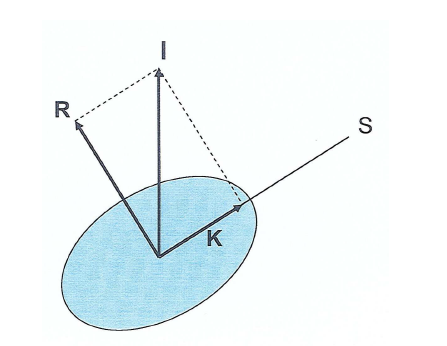
\includegraphics[width=0.7\linewidth]{rotor}
	\caption{Simple Rotor with total angular momentum $I$ of nucleus,
	         a projection of $I$ along symmetry axis, $K$.  }
	\label{fig:rotor}
\end{figure}

Spherical symmetric nuclei의 경우에는 quantum mechanical system에 대해
rotation을 생각하는 것이 어렵다. 어느 특정 방향으로의 rotaion을 생각할 수 없고,
따라서, rotational motion을 생각할 때는 symmetry axis를 축으로 하는 rotation은 
생각하지 않는다. deformed nuclei의 경우 intrinsic spin 의 방향은 symmetry axis와 
평행할 것이고, symmetry axis를 축으로 도는 것은 생각할 수 없다. 대신,
deformed nuclei의 경우에는 symmetry axis에 대해 
수직인 축으로의 rotation을 생각할 수 있게 된다. 
따라서 total angular momentum ${\bm I}$는
rotation ${\bm R}$과 intrinsic spin ${\bm j}$ 의 합으로 생각할 수 있다,
${\bm I}={\bm R}+{\bm j}$. 이 때, axial symmetric nuclei의 경우에는 
${\bm R}$이 symmetry axis에 수직이므로, total angular momentum $I$의 
symmetry axis 에 대한 projection 과 intrinsic spin 의 symmetry axis에 대한
projection을 생각할 수 있고, 이것이 보존된다. 
(여기서, 헷갈리는 것은 Rotation이라는 것이 
핵 전체가 rigid body 처럼 도는 것으로 생각해야 하는지,
아니면, 내부적으로 보이지 않는 핵자들의 flow가 있는 것으로, 
내부적인 flow의 상태가 변하는 것으로 생각해야 하는지 하는 것이다. 
아무래도, 외부적으로 보이지 않는 일종의 내부 flow의 변화로 
rotational state를 이해해야 하는 것이 아닐까 생각된다. 
Rigid body rotation 처럼 생각할 경우, 특정 R 위치에서의
optical potential은 시간에 따라 계속 변해야 하는 반면,
internal flow로 생각할 경우에는 시간에 대한 변화없이
핵의 대칭축과 R vector의 사잇각에 의해서만 결정되고,
이것은 시간에 대해서 변하지 않는다.
다른 말로, 위 그림에서 Rotational excitation에 의해 그림의
핵이 돌아가는 속도가 바뀌는 것으로 생각하기 보다는 
그림의 핵의 모양은 일정한 상태에서 R vector의 크기만
바뀌는 것으로 생각하는 것이다. )



In other words, 
\begin{itemize}
	\item In body fixed frame, the state of a nuclei can be written as $|j K\ra$ where K is a projection 
	      of intrinsic spin on body fixed $z'$-axis. (${\bm j}\cdot\hat{z}'|j K\ra = K|j K\ra$)
	\item Rotation about the body fixed symmetric axis has no meaning in quantum mechanics.       
	      Thus, only perpendicular rotation to body-fixed symmetry axis can be considered. 
	      Thus, $\hat{R}\cdot\hat{z}'=0$. 
	\item In laboratory frame, the total angular momentum(or total spin) of a nucleus 
	      and its projection on laboratory $z$-axis is a good quantum number. $I_z|IM\ra = M|IM\ra$.
	      Also, it's projection on to body fixed $z'$ axis is also a good quantum number,
	      $I_{z'}={\bm I}\cdot{\hat{z}'}={\bm j}\cdot\hat{z}'$. Thus, the rotational state 
	      can be expressed as $|IM K\ra$.   
	\item Rotation can be described as an Euler angle of body fixed $z'$-axis from laboratory $z$-axis.
	      This corresponds to rotation matrix. 
	\item 여기서, IMK 라는 quantum number는 eigen-value로써, time-independent하다. 
	      즉, momentum eigen state $|\vk\ra\sim e^{i\vk\cdot\vr}$ 로 time-dependence를 따로 생각하듯이,
	      $|IMK\ra$ 의 경우도 rotation에 대한 tim=dependence는 따로 생각하고,
	       wave function 의 representation은 $\la \omega|IMK\ra$ 은 오직, intrinsic body-fixed axis와 
	       laboratoty frame의 z-axis 사이의 Euler angle $\omega$ 에만 의존한다. 
	       (angle이 시간에 따라 도는 식 $\theta(t)$로 생각하지 않는다. )    
	\item Transitions occur among states with the same value of $K$.                    
\end{itemize}

Deformed rotating nuclei의 wave function 은 
intrinsic part $\chi_K$와 rotational part, $D$, 로 분리해서 생각할 수 있고,
이 두 부분이 independent 라고 가정하면, wave function은 이 둘의 곱이 된다. 
Lab frame에서의 rotational state는 symmetry axis가 lab frame에서 어느 방향인지를 나타내는 것으로 
나타내어 진다고 볼수 있다.
Total angular momentum $I$인 입자의 transformation property로부터  
rotation motion을 기술하는 wave function은 Wigner D-matrix가 된다고 생각할 수 있다.
(with rank I ) 
또한, spherical symmetry at laboratoray system 에 의해 특정 방향에 대한 
nuclei 의 에너지 차이를 생각할 수 없으므로,$\psi_{I M}$은  $M$에 대해 degenerate
해야하고, 또한 clock-wise motion과 counter clock-wise motion도 degenrate 해야하므로,
$K$와 $-K$에 대해서도 two-fold degeneracy를 가져야 한다. 따라서,
Rotational Nuclei의 Wave function은 
\bea 
\Psi_{IMK}=\left(\frac{2I+1}{16\pi^2}\right)^{\frac{1}{2}}
   \left[ D^{I}_{MK} \chi_K +(-1)^{I-K} D^I_{M-K} \chi_{-K}\right],
\eea  
로 써지게 된다. even-even nuclei의 경우 intrinsic spin이 zero 이므로, $K=0$이 되고,
이것은 $I$가 even인 값(0,2,4..)만이 가능함을 의미한다. odd nuclei의 경우에는 , K의 값이 half-integer, 
이러한 제한이 없다. 특히 $K=0$인 경우는 simply
\bea 
\Psi_{IM0}=\left(\frac{2I+1}{8\pi^2}\right)^{\frac{1}{2}}D^{I}_{M0} \chi_0, \quad (I=0,2,4..)
\eea 


이 때, $|IMK\ra$ state는
\bea 
{\bm I}^2|IMK\ra =I(I+1)\hbar^2|IMK\ra,
\quad I_{z}|IMK\ra =M\hbar|IMK\ra,\quad 
I_{z'}|IMK\ra =K\hbar|IMK\ra
\eea 
를 만족한다.

Rotational energy는 
\bea 
H=\frac{\hbar^2}{2\tau} {\bm R}^2=\frac{\hbar^2}{2\tau} ({\bm I}-{\bm j})^2
 = \frac{\hbar^2}{2\tau}({\bm I}^2+{\bm j}^2-2 I_{z'}j_{z'})+T_{coup} 
\eea 
로 써지고, 여기서 $T_{coup}$는 slow rotation에서는 무시가능하다. 
(${\bm R}$ 이 항상 ${\bm j}$와 수직이고, ${\bm I}={\bm R}+{\bm j}$라면, 
$-2{\bm I}\cdot{\bm j}=-2{\bm j}^2$ 이 될 것 이다. 따라서, $E\sim {\bm I}^2 -{\bm j}^2$. 정말??)


따라서, 간단히
\bea 
E(I)=A I (I+1)+B
\eea 
로 parametrize 할 수 있다. 
단, Moment of inertia는 roational band 에 따라 다른 값을 가질 수도 있고, 
위 식은 단지 낮은 $I$ 값에 대해서만 성립한다. 좀 더 일반적으로는 
\bea 
E(I)=A I(I+1)+B(I(I+1))^2+\dots 
\eea 
를 생각할 수 있다. 

한편, 다음의 세가지 경우에 대해 rotational energy를 생각해 보자. 

(1) even-even nuclei 의 경우 $j=0$, $K=0$이고, band는 $I=0+$ 로 부터 시작되며,
    I는 even 값 $I=2^{+},4^{+},\dots$ 만 가진다. 
    \bea 
    E(I)=\frac{\hbar^2}{2\tau}I(I+1), \quad I=0,2,4,\dots 
    \eea 

(2) odd nuclei with $K\neq \frac{1}{2}$. 이 경우 , band는 $I=K$ 부터 시작하고,
    $I=K+1,K+2,\dots$를 가질 수 있다. (모두 같은 parity를 같는다?)
    \bea 
    E_K(I)=\frac{\hbar^2}{2\tau}[I(I+1)-K(K+1)], \quad I=K,K+1,K+2,\dots 
    \eea 

(3) Odd nuclei with $K=\frac{1}{2}$. 이 경우엔 특별하게, $T_{coup}$ term에 의한 
   mixing 효과를 고려해야 한다. 
   \bea 
   E_{K=\frac{1}{2}}(I)=\frac{\hbar^2}{2\tau}[I(I+1)-a(-1)^{I+\frac{1}{2}}(I+\frac{1}{2})], \quad I=\frac{1}{2},\frac{3}{2},\dots 
   \eea 
   여기서, $a$는 decoupling parameter.

(4) According to A. Bohr, $^{235}U$ levels (odd nuclei) can be parameterized as
\bea 
E(I) = A I(I+1)+ B I^2(I+1)^2+\dots+(-1)^{I+K}\frac{(I+K)!}{(I-K)!}( A_{2K}+B_{2K} I(I+1)+\dots)
\eea 

\subsection{Deformation of potential}
Nuclear Deformation을 생각하면, charge distribution의 change에 따라서
Coulomb interaction이 변형되고 matter distribution의 변화로 
optical potential도 deform이 된다.이러한 변형의 효과는 Coulomb excitation이나 
Collective excitation (Rotation, vibration)에 의한 
nuclear state 변화로 나타나게 된다. 

Deformed nucleus 에 대해서 deformed surface of a nucleus 를 
body-fixed reference frame에서 정의하자. 
\bea 
\tilde{R}(\theta',\phi')
&=&R_0+\sum_{q=2}^{q_{max}} \sum_{\mu=-q}^{q} d_{q\mu} Y_{q\mu}(\theta',\phi')     
\eea 
여기서, parameter $d_{q\mu}$는 length dimension을 가지고, 특별히 
$d_{q0}$는 deformation length $\delta_q$라고 부른다. 
($q=0$는 $R_0$에 포함되고, $q=1$은 translation을 의미한다. Deformation에 대해
Volume이 변하지 않는다 등의 조건을 주면, $d_{q\mu}=(-1)^\mu d_{q-\mu}$를 만족해야한다.
특히 axially symmetric인 경우에는 $q=2$에 대해 오직 $d_{20}$만이 non-zero이다. 
물론 triaxial symmetric인 경우에는 $d_{22}=d_{2-2}$도 non-zero.
) fractional deformation $\beta_q$는 
\bea 
\beta_q=\delta_q/ R_0.
\eea 
로 정의하고 $\beta_2>0$ is prolate, $\beta_2<0$ is oblate라고 부른다.  

아주 단순한 rotational model에서 deformation of optical potential은 
\bea 
V(R,\theta',\phi')&=& U(R-\tilde{R}(\theta',\phi')+R_0)\no 
                  &\simeq& U(R)-U'(R)\sum_{q\mu} d_{q\mu} Y_{q\mu}(\theta',\phi')  
\eea  
{\bf Axially deformed rotator의 경우} $q$는 multipolarity 로 생각할 수 있다.
\bea 
V(R,\theta',\phi')=U(R)-U'(R)\sum_{\lambda=2}^{q}\delta_\lambda Y_{\lambda 0}(\theta',\phi')  
\eea 
여기서 angle은 laboratory vector $\vR$과 body-fixed coordinate에서의 axis $\hat{z}'$
의 angle이므로
\bea 
Y_{\lambda 0}(\theta',\phi')
=\frac{\hat{\lambda} }{\sqrt{4\pi}}P_\lambda(\cos\theta')
=\frac{\hat{\lambda} }{\sqrt{4\pi}}\frac{4\pi}{2\lambda+1}\sum_m 
  Y_{\lambda m}(\hat{\xi}) Y^*_{\lambda m}(\hat{R})
\eea 
따라서,
\bea 
V(R,\hat{\xi},\hat{R})
=U(R)-U'(R)\sum_{\lambda} \delta_\lambda \frac{\sqrt{4\pi}}{\hat{\lambda}}
  \sum_m  Y_{\lambda m}(\hat{\xi}) Y^*_{\lambda m}(\hat{R})
\eea 

This means that in the rotational model,  
\bea 
{\cal F}_\lambda(R)&=&-U'(R),\no 
T_\lambda(\xi) &=& \frac{\delta_\lambda}{\hat{\lambda}} Y_\lambda^*(\xi). 
\eea 

즉, reduced coupling potential은 (여기서는 $\delta_\lambda$는 deformed nucleus
의 intrinsic property 로 상수 취급. 하지만, 일반적으로는 $\hat{\delta}_\lambda$ 는 
$V^\lambda_{fi}(R)= -\frac{1}{\sqrt{4\pi}}\frac{dU(R)}{dR} 
\la I_f||\hat{\delta}_\lambda(\xi)|| I_i\ra$ 로 model dependent 한 양으로 
계산해야 한다.)
위 식을 통해서 potential을 orbital angular momentum dependent part와 
intrinsic part로 분리했다. 여기서, $\hat{\xi}$는 z-축과 body-fixed axis와의 
angle 이므로 시간에 따라 변하는 것으로 생각할 수 있다.  
\bea 
V_{fi}^\lambda(R)={\cal F}_\lambda(R)\la I_f|| {\cal T}(R,\xi)||I_i\ra 
                = -\frac{ d U(R)}{dR}\frac{1}{\hat{\lambda}} 
                  \la I_f|| \delta_\lambda  Y_\lambda(\xi)|| I_i\ra 
\eea 
한편, {\bf Rotor model의 경우},
$Y_{\lambda m}(\xi)=\frac{\hat{\lambda}}{\sqrt{4\pi}} D^\lambda_{m0}(\omega)^*$
이고, rotating state wave function 은 다음과 같이 생각할 수 있다.
Let us consider the rotationally excited state of a rotor $\phi_{IM}$
from intrinsic state $\phi_K$,\footnote{원래는 symmetry 를 고려한 식으로 계산해야한다. } 
\bea 
\phi_{IM}=\frac{\hat{I}}{\sqrt{8\pi^2}} D^{I}_{MK}(\omega)^* \phi_K
\eea 
where $D^I$ is a rotational matrix and $\omega$ is a Euler angles. 
From matrix element,
\bea 
\la I_f M_f|Y^*_{\lambda m}(\hat{\xi})|I_i M_i\ra 
&=&\frac{\hat{I_i}\hat{I_f}}{8\pi^2}\int d\omega 
 \la \phi_K| D^{I_f}_{M_f K}(\omega)Y^*_{\lambda m}(\hat{\xi})
            D^{I_i}_{M_i K}(\omega)^* |\phi_K\ra \no 
&=& \frac{\hat{\lambda}}{\sqrt{4\pi}}\hat{I}_i \la I_i K,\lambda 0| I_f K\ra 
    \hat{I}_f^{-1} \la I_i M_i,\lambda m| I_f M_f\ra ,\no 
\eea 
We get reduced matrix elements, 
\bea 
\la I_f || Y_\lambda^*(\xi) || I_i\ra &=& \frac{\hat{\lambda}}{\sqrt{4\pi}}
                                  \hat{I}_i \la I_i K,\lambda 0|I_f K\ra.        
\eea 
By using the integral of rotational matrix,
\bea 
V_{fi}^\lambda(R)=-\frac{\delta_\lambda}{\sqrt{4\pi}} \frac{ d U(R)}{dR} \hat{I}_i
                  \la I_i K,\lambda 0| I_f K\ra. 
\eea 
따라서, $U(R)$ 이 주어진 경우, deformation length $\delta_\lambda$ 가 input 으로 
필요하다. 

주의할 것은 비록 Coulomb deformation과 비슷한 모양이긴 하지만, 
Coulomb은 charge distribution과 관련되고, 여기서는 nucleus 의 shape deformation
을 생각하므로, 이 둘이 완전히 같지는 않다는 점이다. 
또한, Coulomb excitation의 경우, 
Radial form 이 $1/R^{\lambda+1}$ 인데 비해, Nuclear deformation에 의한 
form factor는 $\frac{dU}{dR}$ form이다. 따라서, Coulomb excitation에 들어가는 $p1$
은 deformation length가 아님. 

\section{Another attempt} 
The surface of collective nuclei which is deformed from spherical shape,
\bea 
R=R_a(\Omega') = R_0\left(1+\sum_{\lambda\mu} a_{\lambda\mu} Y_{\lambda\mu}(\Omega')\right)
\eea 
in body-fixed frame. (To be real $R$, $a^*_{\lambda\mu}=(-1)^\mu a_{\lambda -\mu}$. )
\footnote{If $\lambda=1$, 
$R_a(\Omega')=R_0(1+\sqrt{3/4\pi}{\bm a}\cdot{\bm r}')$
corresponds to overall translation in direction ${\bm a}$.
}
In space fixed frame,
\bea 
R=R_\alpha(\Omega) = R_0\left(1+\sum_{\lambda\mu} \alpha_{\lambda\mu} Y_{\lambda\mu}(\Omega)\right)
\eea 
The spherical Harmonics and coefficients between space-fixed frame and body-fixed frame
are related via Euler angles and rotation matrix. 
\bea 
Y_{\lambda\mu}(\Omega')=\sum_{\mu'} D^{\lambda}_{\mu'\mu}(\omega) Y_{\lambda\mu'}(\Omega)
\eea 
\bea 
\alpha_{\lambda\mu}=\sum_{\mu'} D^{\lambda}_{\mu\mu'}(\omega) a_{\lambda\mu'}
\eea 
Thus, rotation can be described by Euler angles. (In other words, we can see Euler angles 
as internal coordinates of rotational states.)

On the other hand, in case of vibration, we may think the Euler angle is fixed but
the coefficient $a_{\lambda\mu}$ corresponds to vibration and considered 
in terms of internal coordinates.  

With a (small) deformation of spherical potential,
\bea 
V(\vr,\alpha)=V_C(r)+V_N(r)+V_{coup}(\vr,\alpha)
\eea 
where non-spherical part of potential
\bea 
V_{coup}(\vr,\alpha)=V_{coup}^C(\vr,\alpha)+V^N_{coup}(\vr,\alpha)
 =\sum_{LK} v_L(r) \alpha_{L K} Y_{LK}(\Omega)
\eea 
with $v_L(r)=v_L^C(r)+v^N_L(r)$ which can be approximated as derivative of spherical potential. 

For spin coupled states, $|(l I) J M\ra $, one can obtain matrix elements of non-spherical potential as
\bea 
V_{bc}^J(r)&=& \la (l_b I_b)JM| V_{coup}|(l_c I_c)J M\ra \no 
           &=& \sum_{L} (-)^{l_c+I_b+J}\sixjsymbol{J}{I_b}{l_b}{L}{l_c}{I_c}
               \la I_b||\alpha_L||I_c\ra \la l_b||Y_L||l_c\ra  v_L(r) \no 
           &=&\sum_{L} (-)^{l_c+I_b+J+l_b}
             \left(\frac{(2l_b+1)(2L+1)(2l_c+1)}{4\pi} \right)^{1/2}      
             \threejsymbol{l_b}{L}{l_c}{0}{0}{0}
             \sixjsymbol{J}{I_b}{l_b}{L}{l_c}{I_c}
             \no & &\times 
             \la I_b||\alpha_L||I_c\ra v_L(r) 
\eea 
Thus, one can compute the collective excitation by computing $\la I_b||\alpha_L||I_c\ra $. 
In case of rotation, $\alpha_{\lambda\mu}$ is related with $a_{\lambda\mu'}$
of body-fixed frame through rotation matrix. In case of vibration, we can treat the
$\alpha_{\lambda\mu}$ as an operator. 
 
\subsection{rotational excitation}
we have to specify quantum numbers of rotational states $|I_c\ra$ and its energy levels
in rotational model and then compute the matrix elements with $\alpha$.

For permanently axially deformed nuclei,
\bea 
a_{\lambda\mu}=\beta_\lambda \delta_{\mu 0}
\eea 
and related with space fixed one
\bea 
\alpha_{\lambda\mu}=\beta_\lambda D^\lambda_{\mu 0}(\omega)
\eea 
Consider rotation of axially symmetric nucleus about a space-fixed axis with total spin I and spin projection K. (rotation corresponds to change of Euler angle. there is no rotation in body-fixed frame.)
Projection on the body-fixed axis, K,  is also a conserved quantum number. Thus,
rotational state is described as $|I M K\ra$.

Simplest case of structureless nucleus with moment of inertia ${\cal J}$ rotating about 
an axis perpendicular to the symmetry axis. this implies $K=0$ and $I=$even. 
\bea 
\frac{\hbar^2}{2{\cal J}} {\bm I}^2|IM0\ra &=& \frac{\hbar^2}{2{\cal J}} I(I+1)|IM0\ra \no 
I_z |I M 0\ra &=& M |I M 0\ra 
\eea 
In coordinate representation is a function of Euler angles ,
\bea 
\la \alpha,\beta,\gamma=0| I M 0\ra = \left(\frac{2l+1}{4\pi}\right)^{1/2} D^{I}_{M0}(\alpha,\beta,0)
 =(-)^M Y_{IM}(\beta,\alpha)
\eea 
Note that we have to consider it as a wave function of rotational state 
in all Euler angles $(\alpha,\beta)$ instead of thinking the Euler angle is fixed in space
as physical rotation. (Just like the quantum rotational state $|Lm\ra$ 
has wave function $Y_{LM}(\theta,\phi)$ in space. One should not consider classical rotation
as a function of time. )

\bea 
\la I_b||\alpha_L||I_c\ra = \beta_L \la I_b||D^{L}_{00}||I_c\ra 
                         = \beta_L (-)^{I_b}\la I_b 0|D^L_{00}|I_c 0\ra 
                           \threejsymbol{I_b}{L}{I_c}{0}{0}{0}^{-1}
\eea 
where $D_{00}$ is chosen because reduced matrix element does not depends on projection.
\bea 
\la I_b 0| D_{00}^L|I_c 0\ra = \sqrt{\frac{4\pi}{2L+1}}\int d\Omega Y_{I_b 0}(\beta,\alpha)
                                 Y_{L0}(\beta,\alpha) Y_{I_c 0}(\beta,\alpha)
\eea 

\subsection{Vibrational excitation}
Because the wave function of potential matrix element is space-fixed ones,
one have to work in the space-fixed system. Parameter $\alpha_{\lambda\mu}$
are intrepreted as elongation operators which is self-adjoint. 
\bea 
\alpha_{\lambda\mu}^\dagger = (-)^\mu \alpha_{\lambda,-\mu},\quad 
\pi^\dagger_{\lambda\mu}=(-)^\mu \pi_{\lambda,-\mu}
\eea 
 where $\pi$ is a cannonically conjugate momentum satisfying,
\bea 
\left[ \alpha_{\lambda\mu},\pi_{\lambda'\mu'}\right] &=& i\hbar \delta_{\lambda\lambda'}\delta_{\mu\mu'}\no 
\left[\alpha_{\lambda\mu},\alpha_{\lambda'\mu'}\right]&=&\left[\pi_{\lambda\mu},\pi_{\lambda'\mu'}\right]=0.
\eea  
the vibrational Hamiltonian is (In other words $\alpha$ corresponds to displacement $x$.)
\bea 
h =\sum_{\lambda\mu}\left(\frac{1}{2B_\lambda}\pi^\dagger_{\lambda\mu}\pi_{\lambda\mu}
    +\frac{C_\lambda}{2}\alpha_{\lambda\mu}^\dagger \alpha_{\lambda\mu} \right) 
\eea   
Re-organize Hamiltonian in terms of creation and annihilation operators,
\bea 
c_{\lambda\mu}&=&(\frac{ B_\lambda\omega_\lambda}{2\hbar})^{1/2} \alpha_{\lambda\mu}
                +i(-)^\mu(\frac{1}{2\hbar B_\lambda\omega_\lambda})^{1/2} \pi_{\lambda,-\mu}  \no 
c^\dagger_{\lambda\mu}&=&(-)^\mu(\frac{ B_\lambda\omega_\lambda}{2\hbar})^{1/2} \alpha_{\lambda-\mu}
                -i(\frac{1}{2\hbar B_\lambda\omega_\lambda})^{1/2} \pi_{\lambda,\mu}, 
                \omega_\lambda = (\frac{C_\lambda}{B_\lambda})^{1/2}
\eea 
or conversely
\bea 
\alpha_{\lambda\mu}&=&(\frac{\hbar}{2B_\lambda \omega_\lambda})^{1/2}\left(c_{\lambda\mu}+(-1)^\mu c^\dagger_{\lambda,-\mu} \right) 
\eea 
with 
\bea 
\left[ c_{\lambda\mu},c^\dagger_{\lambda'\mu'}\right] &=&  \delta_{\lambda\lambda'}\delta_{\mu\mu'}\no 
\left[c_{\lambda\mu},c_{\lambda'\mu'}\right]&=&\left[c^\dagger_{\lambda\mu},c^\dagger_{\lambda'\mu'}\right]=0
\eea 
\bea 
h = \sum_{\lambda\mu} h\bar\omega_\lambda(c^\dagger_{\lambda\mu} c_{\lambda\mu}+\frac{1}{2}).
\eea 

Thus, vibrational state can be specified with $|n;I M_I\ra$. 
One can have  one-phonon state from mode $\lambda=I$,
\bea 
|n=1;I m_I\ra = c^\dagger_{I M_I}|0\ra 
\eea 
or two-phonon state from modes $\lambda_1$ and $\lambda_2$,
\bea 
|n=2; I M_I\ra =\frac{1}{\sqrt{1+\delta_{\lambda_1\lambda_2}}}
	     \sum_{\mu_1\mu_2} \la \lambda_1 \mu_1 \lambda_2 \mu_2|I M_I\ra 
	         c^\dagger_{\lambda_1\mu_1}c^\dagger_{\lambda_2\mu_2}|0\ra
\eea 
and so on. 
With this in mind, the coupling matrix element between two vibration states is
\bea 
\la n_b;I_b||\alpha_L|| n_c;I_c\ra 
&=& (\frac{\hbar}{2B_L\omega_L})^{1/2}(-)^{I_b}\threejsymbol{I_b}{L}{I_c}{0}{0}{0}^{-1}
    \la n_b; I_b 0|(c_{L0}+c_{L0}^\dagger)|n_c;I_c 0\ra. \nonumber 
\eea 

for example, between zero-phonon and one-phonon state,
\bea 
\la 0;0||\alpha_L||1;I\ra = (\frac{\hbar}{2B_I\omega_I})^{1/2}(-)^{I}(2I+1)^{1/2} \delta_{LI}. 
\eea 

One can replace $(\frac{\hbar}{2B_I\omega_I})$ 
in the Coulomb part of the interaction with $B(EI)$ value for the one-phonon transition.
\bea 
B(E1;1\to 0)=(\frac{3}{4\pi} Z_t e R_C^I)^2 (\frac{\hbar}{2B_I\omega_I})
\eea 
then,
\bea 
\la 0;0||\alpha_L||1;I\ra = (-)^I (2I+1)^{1/2} \delta_{LI}\frac{4\pi}{3 Z_t e R_c^I}[B(EI;1\to 0)]^{1/2}
\eea 

\subsection{Coulomb polarization potential}
(REF: Book of Froblich et al)

Consider one-step Coulomb excitation from ground state to $|I M\ra$ states, $M=-I,\dots I$. 
(In other words $P=|00\ra\la 00|$ and $Q=\sum_m|I m\ra\la Im|$. )
In this simple model space, one can compute the GOP as 
\bea 
{\cal V}=V_0+\la 0|V|0\ra+\la 0|V Q \frac{1}{E+i\eta-T-h-V} Q V|0\ra 
        \simeq V_0 +V_{pol}
\eea 
here $V_0=V_c+V_N$ is the real static Coulomb+nuclear potential. 
(In other words, here we are computing equivalent local potential 
with full coupled channel calculation.)
Diagonal $\la 0|V|0\ra $ is small. 
Coulomb polarization potential is complex non-local energy-dependent.
(Previous polarization potential was meant to be real potential
comes from dispersion relation.) 

With many simplification/approximation, (treat the solution as plane wave),
trivially equivalent local potential is 
\bea 
V_{pol}(r) = -\frac{2I+1}{16\pi E} V_I(r)[V_I(r)+ 2ik F_I(r)]
\eea 
where
\bea 
V_I(r) = \frac{4\pi Z_p e}{R_C^I (2I+1)^{3/2}}[B(EI;0\to I)]^{1/2} \frac{r_{<}^I}{r_{>}^{I+1}} 
\eea 
\bea 
F_I(r)=2\pi^2\int_0^\infty q dq j_I(qr)\tilde{V}_I(q)
\eea 

Leading term in the Couomb polarization potential is the $I=2$ contribution, and at large r,
\bea 
\mbox{Re} V_{pol}(r) = -\frac{\pi}{25}\frac{B(E2;0\to 2)}{E}\frac{Z_p^2 e^2}{r^6}
\eea 
\bea 
\mbox{Im} V_{pol}(r) &=& -\frac{2}{3}\frac{\omega_{pol}}{R_C^9}r^4 ,\quad \mbox{for } r< R_C,\no 
                &=& -(1-\frac{2}{7}\frac{R_C^2}{r^2}-\frac{1}{21}\frac{R_C^4}{r^4}) \omega_{pol} \frac{1}{r^5}, \quad \mbox{for } r> R_C,
\eea 
with 
\bea 
\omega_{pol} = \frac{4\pi}{75}\frac{2\mu}{\hbar^2 k} Z_p^2 e^2 B(E2;0\to 2)
\eea 

\subsection{Nuclear Moments}
Let us define more clearly on the nuclear moments. 
Keep in mind that there can be electric nuclear moments
(which is related with charge/magnetic distribution)
and matter nuclear moments which are in general different. 
\begin{itemize}
\item Nuclear Mean Squared Charge Radius: second radial moment
     of nuclear charge
     \bea 
     \la r^2\ra =\frac{\int_0^R \rho(\vr)\vr^2 d\vr}{\int_0^R \rho(\vr)d\vr}
     \eea
     If the shape is axially deformed, we have charge deformation 
     parameter $\beta_2$ as
     \bea 
     R(\theta)=R_1[1+\beta_2 Y_{20}(\theta)],
     \eea  
     Liquid drop model gives
     \bea
     \la r^2\ra &=& \frac{3}{5}R^2+\frac{3}{4\pi}R^2\beta^2_2 \no 
                &\to& \la r^2\ra_{sph}
                     +\frac{5}{4\pi}\la r^2\ra_{sph} \beta^2 
     \eea 
\item magnetic moment operator of nuclei: sum of free nucleon
      magnetic moments with gyromagnetic factors
     \bea 
     \hat{\bm \mu}=\sum_{i=1}^A g_l^i {\bm l}^i
                  +\sum_{i=1}^A g_s^i {\bm s}^i
     \eea
     Magnetic dipole moment of nuclei $\mu_I$ (which is dependent on the spin state of nucleus)
     is 
     \bea 
     \mu_I=\la I,m=I|\hat{\mu^z}|I,m=I\ra 
     \eea      
     and nuclear spin ${\bm I}$ is related to the gyromagnetic ratio
     \bea
     {\bm \mu}=g_I {\bm I} \mu_N 
     \eea 
\item Electric Quadrupole moment: 
      electric quadrupole moment operator can be defined as
      \bea 
      \hat{\bm Q}_2^0=\hat{\bm Q}_z=\sqrt{\frac{16\pi}{5}}\sum_{i=1}^A
                       e_i r_i^2 Y_{20}(\hat{r}_i) 
      \eea      
      Spectroscopic quadrupole moment of nuclear spin I is
      \bea 
      Q_s(I)&=&\la I,m=I|\hat{\bm Q}_2^0|I,m=I\ra 
              =\hat{I}^{-1}\la II,20|II\ra \la I || {\bm Q} || I\ra \no  
            &=&\sqrt{\frac{I(2I-1)}{(2I+1)(2I+3)(I+1)}}
             \la I || {\bm Q} || I\ra 
      \eea 
      (Note spectroscopic quadrupole moment is zero if I$<$1
      even with deformed nucleus with spin is 0 or 1/2.
      )
      
      
\item Intrinsic quadrupole moment $Q_0$ is related to the intrinsic 
      deformation $\beta_2$. The $Q_s$ and $Q_0$ can be related 
      only in a certain assumptions. Axially symmetric nuclei case,
      \bea 
      Q_s(I)=\frac{3K^2-I(I+1)}{(I+1)(2I+3)} Q_0
      \eea 
      with K being the projection of nuclear spin on the 
      deformation axis. 
      Intrinsic quadrupole moment in a small deformation $\beta_2$
      is related as
      \bea 
      Q_0=\frac{3}{\sqrt{5\pi}}ZR^2\beta_2(1+{\color{red}0.36}\beta_2)
      \eea 
      If matter distribution is considered we may replace $Z\to A$.
      (RIPL used 0.16 instead of 0.36 ? and $R=1.2A^{1/3}$ fm.)
\end{itemize}
 




\subsection{Fresco: deformation}
FRESCO에서 collective exciation의 효과를 넣는 방법이 여러가지가 있다. 
Coulomb deformation의 경우와 nuclear deformation의 경우를 따로 생각해야 한다. 

\begin{itemize}
\item \&POT 에서 deformation length를 input으로 주는 경우.
      (TYPE=10,11) 
\item \&POT 에서 \&STEP 을 이용하여, matrix element를 주는 경우.(TYPE=12,13).
       (단, 이때에는 
       $I_i\to I_f$ 뿐 아니라 $I_f\to I_i$ 도 explicit하게 주어야 한다. )
\item \&COUPLING 에서 \&INEL 을 이용하여 coupling을 define하는 경우.        
\end{itemize}

Information of deformation is described in Potentials 
(Type=10,11, Shape=7,8,9)of FRESCO input.

Nuclear deformation에 대해 $P(k)=DEF(k)$ corresponds to 
deformation length in fm ($\delta_\lambda$). 

Coulomb deformation에 대해서는 $P(k)=Mn(Ek)$ corresponds to
the instrinsic reduced matrix elements in $e.fm^k$ units. 
이 때, $Mn(Ek)$는 
\bea 
Mn(Ek)=\frac{\la I'||Ek||I\ra}{\sqrt{2I+1}\la I K,k0|I' K\ra} 
\eea 
로 정의 되는데, 이 때 $\la I'||Ek||I\ra$는 Alder and Winther의 definition을 따른다.  
\bea 
Mn(Ek)=\frac{3 Z\beta_k R^k}{4\pi}
\eea 
이것은 앞에 사용된 식과 일치하는 것으로 보인다. 
(RIPL 에 의하면, E.M. deformation parameters are extracted from measured $B(E\lambda)$ as
\bea 
B(E\lambda) = \left(\frac{3 R_0^\lambda Z}{4\pi}\beta_\lambda\right)^2,\quad R_0=0.12 A^{\frac{1}{3}}\quad [\sqrt{b}].
\eea 

 )


주의할 것은 Type에 따라, SHAPE에 따라 $P(k)$의 의미가 달라짐. 

Fresco manual에 typo가 있는 것으로 생각된다. 
{\color{red} Coulomb deformation 의 경우, TYPE=10,11 일 때의 입력값 $P(k)$ 는 $M_n(Ek)$ 가 맞는 것으로 보인다.}
실제 포텐셜 계산에선, 필요한 factor를 자동으로 곱하여  $M_n(Ek)\to M(Ek)$ 로 바꾸어서 계산하는 것으로 여겨진다. 


\subsection{Inelastic scattering: single particle excitation}
we may consider excitation of a nucleus by a transition of a 
single valence particle state from $\phi_{l_i s j_i}$ to $\phi_{l_f s j_f}$,
or $(I_c j_i)I_i$ to $(I_c j_f)I_f$ with core spin $I_c$.

Let us consider three interaction $V_{cv}(\vr)$, $V_{vt}(\vr_{vt})$, 
$V_{ct}(\vr_{ct})$. 이경우에는 projectile($p=c+v$) 의 excitation 을 생각한다.
For given $\vR$, 
$\vr_{vt}=\vR+\frac{m_c}{m_p}\vr$
and $\vr_{ct}=\vR-\frac{m_v}{m_p}\vr$. $m_p=m_c+m_v$.
\bea 
V_{fi}(R)=\la (L_f J_f)\Lambda|V_{vt}+V_{ct}|(L_i J_i)\Lambda\ra, 
\eea 
$\Lambda=L+J$ is a conserved total angular momentum. 
by the expansion, $z=\hat{R}\cdot\hat{r}$
\bea 
V_{vt}+V_{ct}=\sum_{\lambda}(2\lambda+1){\cal F}_\lambda(R,r) P_\lambda(z)
             =4\pi \sum_{\lambda}{\cal F}_\lambda(R,r)
              \sum_{m} Y_{\lambda m}(\hat{r})^* Y_{\lambda m}(\hat{R})
\eea 
where,
\bea 
{\cal F}(R,r)=\frac{1}{2}\int_{-1}^{+1}[ V_{vt}(r_{vt})+V_{ct}(r_{ct})]P_\lambda(z) dz
\eea 

Thus,
\bea 
V_{fi}^\lambda(R)
=\left( \int_0^\infty u_{l_f s j_f}(r) {\cal F}_\lambda(R,r) u_{l_i s j_i}(r) dr\right)
  \hat{\lambda}\hat{l_i} \la l_i 0,\lambda 0|l_f 0\ra. 
\eea 

\section{single particle transfer} 
 
Stripping example, $p(=n+c)+c'\to n+t'(=n+c')$, 
 \bea 
 & &[ H_p-\epsilon_p]\phi_p(\vr)=0, \quad H_p=T_r+V_p(\vr),\no 
 & &[ H_t-\epsilon_t]\phi_t(\vr')=0, \quad H_t=T_{r'}+V_p(\vr')
 \eea 
Full Hamiltonian can be written in two ways,
\bea 
H&=&T_{\vr}+T_{\vR}+V_p(\vr)+V_t(\vr')+U_{cc'}(\vR_c)\no 
 &=&H_{prior}=T_{\vR}+U_i(R)+H_p(\vr)+{\cal V}_i(\vR,\vr)\no 
 &=&H_{post}=T_{\vR'}+U_f(R')+H_t(\vr')+{\cal V}_f(\vR',\vr')
 \eea 
 where
\bea 
{\cal V}_i(\vR,\vr)&=& V_t(\vr')+U_{cc'}(\vR_{c})-U_i(R) \no 
{\cal V}_f(\vR',\vr')&=& V_p(\vr)+U_{cc'}(\vR_{c})-U_f(R') 
\eea 
Consider Model space, (only two channel)
\bea 
\Psi=\left[\phi_p(\vr)\otimes Y_L(\hat{R})\right]_\Lambda \chi_i(R)/R
    +\left[\phi_t(\vr')\otimes Y_{L'}(\hat{R}')\right]_\Lambda \chi_f(R)/R
\eea 
We need to compute matrix element,
\bea 
\la \left[\phi_t(\vr')\otimes Y_{L'}(\hat{R}')\right]_\Lambda|
               {\cal V}_x |\left[\phi_p(\vr)\otimes Y_L(\hat{R})\right]_\Lambda\ra (R,R')
\eea  

\subsubsection{Details on the calculation}
In general the matrix element becomes a non-local operator.
We can simplify the integral by change of variable and angle integrations. 
\bea
\vr=p\vR'+q\vR,\quad \vr'=p'\vR'+q'\vR 
\eea 
\bea 
p&=&-\omega, \quad q=\nu_t \omega, \quad p'=-\nu_p\omega,\quad q'=\omega,\no 
\nu_p&=&m_c/m_p,\quad \nu_t=m_{c'}/m_{t'},\quad \omega=(1-\nu_p\nu_t)^{-1} 
\eea  
Convert functions $\phi_t(\vr')$ and $\phi_p(\vr)$ into a function of $\vR$ and $\vR'$,

Moshinsky solid-harmonic expansion:
When $\vr=a \vR+b \vR'$, we can expand the spherical harmonics as
\bea 
Y_{lm}(\hat{r})&=&Y_{lm}(\widehat{a \vR+b \vR'}) \no 
      &=&  \sqrt{4\pi} \sum_{n\lambda} 
           c(l,n) \frac{(aR)^{l-n}(bR')^n}{r^l} Y_{l-n,m-\lambda}(\hat{R})
           Y_{n,\lambda}(\hat{R}')
           C^{lm}_{l-n m-\lambda, n\lambda}, \no 
c(l,n)&=&\sqrt{\frac{1}{2n+1}\left(\begin{array}{c} 2l+1 \\ 2n \end{array} 
   \right) }            
\eea 

\bea 
r^2&=& p^2 R^{'2}+q^2 R^2+2 p q R R' z, \quad z=\hat{R}\cdot\hat{R}'\no 
r^{'2}&=& p^{'2} R^{'2}+q^{'2} R^2+2 p' q' R R' z
\eea 


zero-range approximation
\bea 
V^{L}_{l'L';0L}(R',R)=D_0\frac{(-1)^{L'-l'}}{\hat{L}} 
 \frac{\hat{l'_i}\hat{L}\hat{L'}}  {\sqrt{4\pi}}\threejsymbol{l'}{L}{L'}{0}{0}{0}
 \frac{u_{l'}(R')}{R'}
 \frac{q^2}{p}\delta(pR'+qR)  
\eea 

\subsubsection{overlap}

Here, we ignored the unchanged core-internal wave function. 
In fact, we need to consider overlap wave function which 
should be intrinsically many-body,
\bea 
\Psi_{A;B}(r)=\la \psi_A(r,\xi_B)|\psi_B(\xi_B)\ra 
\eea 


 
If target or projectile is a bound state of core(spin $I_c$)+valence($j_v$)
with total $JM$, the bound state wave function 
in coupling order $|(ls)j,I_c;JM\ra$,
can be written as
\bea 
\phi_{JM}(\xi)&=&\phi_{JM}(\xi_c,\vr_{v})
=\sum_{l j I} A^{j_v I_c J}_{l s j_v}
    [ \phi_{I_c}(\xi_c)\otimes \phi_{l_v s_v j_v}(\vr_v)]_{JM}
\eea 
where, bound state wave function can be a linear combination of 
several normalized single particle wave functions as
\bea 
\phi_{l_v s_v j_v}(\vr_v)
= [Y_{l(\hat{r}_v)}\otimes \phi_{s}]_{j_v}\frac{u_{lsjI}(r_v)}{r_v}.
\eea  
And the $A^{j_v I_c J}_{l s j_v}$ is called 
coefficient of fractional parentage(=spectroscopic amplitude) 
for single particle  state in bound state with $JM$. 
$|A^{j_v I_c J}_{l s j_v}|^2$ are called spectroscopic factor.
Note that $u$ are normalized wave functions. 
If there is only one single particle states
for given excited state, c.f.p$=1$ for pure single particle state. 
In fact, we have to anti-symmetrize the total wave function. Thus,
in that case spectroscopic amplitude have to contain factors related with 
anti-symmetrization. 

한편, seperation energy 에 대한 정보로 부터, 
우리는 asymptotic form of bound state wave function 이 Whittaker function에 
비례할 것으로 볼 수 있다. 이 때의 비례 상수를 Asymptotic normalization constant 라고 부른다.
\bea 
\phi_l(r)=_{r>R_n} C_l W_{-\eta,l+1/2}(-2k_p r)\simeq C_l e^{-k_p r}
\eea  
만약, $\phi_l(r)\sim A u_l(r)$ 에서 spectroscopic amplitude $A$와 normalized wave function
으로 쓴다면, normalized wave function 자체가 single particle ANC를 가지고, 
$(ANC)=(s.a.)(s.p.ANC)$ 로 생각할 수 있다. 

The single particle wave functions can be determined by binding potential
between core and valence. Note that in general,
there will be non-zero off diagonal coupling potentials which
connects between excited states. 
Thus, it is enough to specify binding potential and 
single particle state quantum number and c.f.p 
to obtain overlap function $K_{ij}$. 

Transfer reaction 경우, $A(a,b)B$ with 
$a=b+x$, $B=A+x$, coupling potential을 생각해보자. 
DWBA formalism 에서 계산해야하는 coupling은 $\la bB|\Delta V| a A\ra$ 로 
쓸 수 있고, $\Delta V$는 interaction 중 diagonal part가 빠진 potential이다. 
즉, $\la a A|\Delta V| a A\ra =0$ 또는 $\la b B|\Delta V| b B\ra=0$. 
Cluster model에서의 모든 interaction은 아래와 같이 주어진다.
\bea 
H_I&=& V_{xb}+V_{bA}+V_{xA}
\eea 
이 때, entrance channel 을 기준으로 생각하면, $a=b+x$ 이므로, $V_{xb}$ 는 bound state 의 
internal 에 이미 포함되어 있다. 또한, $aA$ 의 elastic scattering 은 optical potential 
$U_{aA}$ 로 기술되므로, 이부분을 빼주어야한다. 따라서, entrance channel을 기준으로 할 때,
(Prior Form)
\bea 
\Delta V^{prior}= V_{x A}+ [ V_{bA}- U_{aA}]
\eea 
라고 쓸 수 있는데, 마지막의 core-core interaction 과 optical potential의 차이를 
Remnant potential 이라고 부른다. 만약 $x$가 core $b$나 $A$에 비해 작은 경우라면,
$V_{bA}-U_{aA}\simeq 0$로 approximation할 수 있고, 이 경우 transition coupling은 
exit channel에서의 binding potential $V_{xA}$ 가 된다. 

마찬가지로, exit channel을 기준으로 하면,(Post form),
$V_{xA}$ 는 bound state $B$에 이미 포함되므로,
\bea 
\Delta V^{post} = V_{x b}+[ V_{bA}-U_{bB} ]
\eea 
라고 쓸 수 있고, 이 경우 remnant potential을 무시하면, 
entrance channel에서의 binding potential $V_{xa}$ 가 transition potential이 된다. 
\footnote{
{\bf Q:} Suppose the inputs does not have optical potential
between $U_{t-p}$, but only have $V_{c-p}$ and $V_{v-p}$. 
In this case, FRESCO automatically computes $U_{t-p}$ from 
$V_{c-p}$ and $V_{v-p}$ and subtract $U_{t-p}$ for 
coupling potential? Or, only considers Coulomb interaction 
between target and projectile in this channel? 

주의: FRESCO 의 경우, 책이나 매뉴얼의 식은 모두,
s.p. excitation이나 transfer는 scalar potential에 의한 경우만
계산하는 것으로 보인다.
}

In general, the coupling becomes non-local in $R_i$ and $R_f$
and requires finite range of non-locality. In zero-range approximation,
${\cal V}_o \phi(\vr)\sim D_0 \delta(\vr)$, the calculation becomes simpler. 
\footnote{zero-range approximation assumes
(1)Wave function is S-wave only (2) remnant term은 무시가능 (3) potential이 zero-range.
따라서, $\int d^3 r V(\vr)\phi(\vr)=\int d^3 r D_0 \delta^3(\vr)$ 로 생각하여, $D_0$를 얻을 수 있다.
}
Local energy approximation은 zero-range approximation에 
finite range effective radius 에 의한 correction을 하는 것.
\footnote{Local energy approximation assumes (1) wave function은 s-wave only 
(2) potential is not zero-range but have small effective range.
} 
zero-range approximation parameter $D_0$ can be written as\footnote{
Considering s-wave bound state solution of delta function potential,
which have the form $e^{-k_p r}$, we can interpret the $D_0$ as the 
asymptotic strength of wave function. From this, when the 
potential has some small range, it would corresponds to replace
$D_0$ into modified asymptotic strength $D$ of wave function. 
} 
\bea 
D_0&=&\sqrt{4\pi}\int_0^\infty r V_0(r) u_0(r) dr,\no 
u_0(r)&\to& \frac{2\mu_p}{\hbar^2}\frac{1}{\sqrt{4\pi}} D e^{-k_p r}
\eea 
Also, in low energy approximation, 
\bea 
D=\sqrt{4\pi}\int_0^\infty \frac{\sinh(k_p r)}{k_p} V_0(r) u_0(r) dr
\eea 
Gives $D=(1+k_p^2 \rho^2_{eff})D_0$, $k_p^2=2\mu_p\epsilon_p/\hbar^2$,
$\rho_{eff}$ is a measure of mean radius of potential $V_0(r)$. 

{\bf Asymptotic Normalization Coefficient} is defined 
as the asymptoric coefficient $C_l$ of the Whittaker function. 
\bea 
u_l(r)\to C_l W_{-\eta,l+\frac{1}{2}}(-2 k_p r)\simeq C_l e^{-k_p r}
\eea 
Thus, in case of S-wave zero-range approximation,
$C_l=\frac{2\mu_p}{\hbar^2}\frac{1}{\sqrt{4\pi}}D$.
ANC is related with the spectroscopic factor. 

\subsection{Cluster Wave function: two particle} 
Or, if it is a bound state of core and two particles,
for coupling order $|\{L,(l,(s_1 s_2)S)j \} J_{12}, I_c ; J\ra$,
\bea 
\phi_{JM}(\xi)&=&\phi_{JM}(\xi_c,\vr,\rho) \no 
   &=&\sum_{L l S j J_{12} I_c} 
   A^{J_{12}I_c  J}_{L j J_{12}}  
   [\phi_{I_c}(\xi_c)\otimes 
            [  Y_{L}(r)\otimes
            [Y_{l}(\rho)\otimes [\phi_{s_1}\otimes\phi_{s_2}]_S]_j]_{J_{12}}                ]_{JM} 
            \frac{u_{12}(r,\rho)}{r \rho}  
\eea 

where coefficients $A$'s are 
called coefficients of fractional parentage.
If the wave function of two particles are 
given in terms of single particle wave functions in each position,
$\phi_{l_1,s_1,j_1}(r_1)$ and $\phi_{l_2,s_2,j_2}(r_2)$,
they have to be converted by
\bea 
\phi_{12}(\vr_1,\vr_2)
&=& 
 \sum_i c_i |(l_1(i),s_1)j_1(i),(l_2(i),s_2) j_2(i); J_{12} T\ra \no 
&\to& 
 \sum_{u} c_i \sum_{Ll S j}
 |L,(l,(s_1s_2)S)j;J_{12},T\ra 
 \phi^{J_{12}T,i}_{L(l S) j}(r,\rho)
\eea 
with
\bea 
\phi^{J_{12}T,i}_{L(l S) j}(r,\rho)
&=&\la L,(l,(s_1 s_2)S)j; J_{12} T| (l_1,s_1)j_1,(l_2,s_2)j_2;J_{12},T\ra
\no & &\times 
 \la [Y_{L}(\hat{r}) Y_{l}(\hat{\rho}) ]_{\lambda}
  | [\phi_{l_1 s_1 j_1}(\vr_1)\phi_{l_2s_2j_2}(\vr_2)]_{J_{12},T}\ra  
\eea 

\subsection{Knockout reactions}

For example, $^{14}C(p,\alpha)^{11}B$, 여기서 target의 일부가 떨어져 나가고
projectile로 대체되는  경우. 이때 가능한 mechanism은 두가지를 생각할 수 있다.
첫번째는 triton trasnfer
\bea 
\left( {}^{14}C=^{11}B+^3H\right)+p\to {}^{11}B+\left(\alpha=p+^{3}H\right).  
\eea 
두번째는 일종의 $p-\alpha$ exchange,
\bea 
\left( {}^{14}C=^{10}Be+\alpha\right)+p\to \left(^{11}B=p+^{10}Be\right)+\alpha
\eea 
두번째 경우에는 exchange 효과를 고려하여 amplitude를 합해야한다. 
단, transition potential, 
${\cal V}_i=V_{p-Be}+U_{p\alpha}-U_{pC}$ , 에서 보통은 첫번째 binding potential
이 중요하여 remnant interaction이 무시됨에 비해서, 이 경우는 $p-\alpha$ interaction 
이 중요해진다. 

\subsection{Continuum: Break up }
If the particle transfers to continuum,
and the coupling with continuum states are important, 
it have to be specified by 'bin' wave functions 
in CDCC method in FRESCO. (Coupling between bound state and continuum 뿐 아니라
coupling between continuum 까지 고려하는 경우)

\subsection{Capture}
penetrability factor. 
direct capture by emission of photon. Or
doorway resonances. compund nucleus by long resonance. 

\subsection{Charge exchange reactions}
Charge exchange 의 경우 다양한 reaction mechanism 이 가능하다. 
예를 들어 $^{12}C(p,n)^{12}N$ 의 경우
\begin{itemize}
	\item heavy-particle transfer of $^{11}C$ from, $^{12}C=^{11}C+n$ to 
	        $^{12}N=^{11C}+p$
	\item two-step transfers via $^{11}C+d$ intermediate state. 
	        $^{12}C+p\to ^{11}C+d\to ^{12}N+n$
	\item direct conversion of a proton to neutron via isospin dependent interaction(like pion exchange)                
\end{itemize}
마지막의 경우는 Lane poential
\bea 
V(R)=V_0(R)+\frac{{\bm t}\cdot{\bm T}}{A} V_T(R)
\eea 
로 표현된다. 

Fermi transition : $H_F=V_F(R){\bm t}\cdot{\bm T}$

Gamow-Teller transition: $H_{GT}=V_{GT}(R)({\bm s}\cdot{\bm S})({\bm t}\cdot{\bm T})$

Generalized multipole transitions

\subsection{Photo-nuclear couplings}

\section{Structure Models}

\subsection{Shell Model}
\subsection{Cluster Models}
\subsection{Mean Field Models}
Hartree theory
\bea
& &[\hat{T}_\vr+V_{mean}(\vr)]\phi_i(\vr)=\epsilon_i \phi_i(\vr),\no
& &\rho(\vr)=\sum_{i=1}^{F} n_{occ}(i)|\phi_i(\vr)|^2,\quad \sum_i n_{occ}(i)=A,\no 
& &V_{mean}(\vr)=\int d\vr' V_{NN}(\vr-\vr')\rho(\vr')
\eea 
Hartree-Fock theory use slater determinant of wave function and exchange term in the equation. 

The density-dependent effective interaction is often used, $V_{NN}(\vr;\rho)$.

Mean-field models are simpler for even-even nuclei, as then nucleons are in pairs
of time-reversed orbits.(?) 

Mean-field models may be used to predict bound-state wave functions for transfer or capture scattering calculations according to the orbital occupation numbers. 

Mean-field are for ground state. For excited states, time-dependent analysis
(Time-dependent Hartree-Fock)
or linear perturbation analysis(Random Phase Approximation) is used.


\subsection{Collective nuclear-matter description}
Use plausible form of $\rho(\vr)$.

Laboratory density depends on the angular momentum $I\mu$.

Body-fixed densities are intrinsic and only depends on the K, which is the projection of intrinsic spin on the body-fixed $z'$ axis.
(Nuclear spin in Laboratory frame is a vector 
sum of intrinsic spin and rotation of the body-fixed axis(${\bm I}={\bm s}+{\bm L}_r$).   

Mean-field, density-functional, 
collective rotation model gives nuclear wave functions initially in body-fixed frame.
Thus, if we want density in lab frame, we need to rotate the wave function. 

Shell model wave usually projected onto good angular-momentum states in laboratory frame. 

We can think of 'matter' deformation in a similar way as 'potential' deformation. 
\bea
\rho(r,\theta',\phi')&=&\rho_0(r-\tilde{R}(\theta',\phi')+R_0),\no 
\tilde{R}(\theta',\phi')&=&R_0
 +\sum_{\lambda=0}^{\lambda_{max}}\sum_{\mu=-\lambda}^{\lambda}\delta_{\lambda\mu}Y_{\lambda\mu}(\theta',\phi')
\eea
$\delta_{\lambda\mu}$ 'matter deformation length', 
fractional matter deformation($\beta_{\lambda\mu}=\frac{\delta_{\lambda\mu}}{R_0}$)
can be defined. 

'intrinsic quadropole moment' for diagonal transitions ($I_i=I_f=I$) and $\lambda=2$,
\bea 
Q&=&\sqrt{\frac{16\pi}{5}}\la \Phi_{JJ}|\hat{Q}_{20}|\Phi_{JJ}\ra \no 
 &=&\sqrt{\frac{16\pi}{5}}\la \Phi_{JJ}|\int d\vr' r^{'2}\hat{\rho}(\vr')Y_{20}(\hat{r}')|\Phi_{JJ}\ra
\eea
\bea 
Q_2= \sqrt{\frac{16\pi}{5}} \frac{\la I I 20|II\ra}{\sqrt{2I+1}}\la I|| M(E2)||I\ra 
\eea 
여기서, $|\Phi_{JM}\ra $ 은 deformed nucleus 의 lab frame에서의 wave function
인 반면 $\rho(\vr')$은 body-fixed frame에서의 matter density 이다.  
\bea 
Q=\frac{3R_0 A}{\sqrt{\pi}}\delta_{2}
\eea 

{\bf example:} If nuclus is a spherical core + unpaired single nucleon, $\phi_{lsj}$,
the quadropole moment is determined by the single particle. Then,
\bea
Q_{sp}=-\frac{2j-1}{2(j+1)}\la r^2\ra,
\quad \la r^2\ra =\int r^2 |\phi_{lsj}(\vr)|^2 d\vr .
\eea 

\section{Overlap functions}

one-body overlap function for transfer, captures or single particle excitation 
involving nucleus B which is core $A$+ single particle,
which is related with spectroscopic amplitude(or c.f.p.). 
중요한것은 overlap function이 일반적으로 간단한 single particle wave function이 아닌,
복잡한 many-body wave function의 일부라는 것이다. 
일반적인 shell model에서도 configuration mixing을 고려할 경우, overlap function은 단순한 
single particle wave function으로 기술되지 않는다. 

만약 antisymmetrization을 고려하지 않으면, A nuclei와 A-1 nuclei의 overlap은
\bea 
\Psi^A_i=\sum_{flj} \phi_{i,f,l,j}(\vr) \Psi^{A-1}_f,\quad
\la \Psi_f^{A-1}|\Psi_i^A\ra(\vr)=\sum_{l,j}\phi_{i,f,l,j}(\vr).
\eea 
와 같이 생각할 수 있다.여기서, i와 f는 A와 A-1 nucleus 의 모든 양자수를 나타낸다. 
즉, overlap function은 가능한 모든 configuration mixing 을 모두 고려하여야한다. 
하지만, 많은 경우 overlap function이 오직 하나의 single particle wave로 
근사 가능하다는 가정을 한다. 

\subsection{Non-antisymmetrized theory: Pauli principle이 무시되는 경우}





Suppose $B=A+v$, core wave $\Phi_{I_A}^A(\xi_A)$ and composite wave function,
$\Phi^B_{I_B}(\xi_B=\{\xi_A,\vr\})$
( 여기서, $\vr$은 single particle과 
core 사이의 위치벡터),
Overlap function,
\bea 
\phi_{I_A:I_B}(\vr)&=&\la \Phi^A_{I_A}(\xi_A)|\Phi^B_{I_B}(\xi_A,\vr)\ra, \no 
\Phi^B_{I_B}(\xi_A,\vr)&=&\sum_{I_A} \phi_{I_A:I_B,nlj}(\vr)\Phi^A_{I_A}(\xi_A).
\eea 
여기서, $I_A$와 $I_B$는 처음과 나중의 모든 물리적인 값을 포함하는 것이고,
$\phi_{I_A:I_B}$ 는 일반적으로 $I_A$와 $I_B$외에도 valence 입자의 $n,l,j$ 에도
의존한다. 
$\phi_{I_A;I_B}(\vr)$ 은 복잡한 manybody problem을 풀어야 얻을 수 있고, 
$\phi_{I_A:I_B}(\vr)$ 각각은 normalize가 되지 않았으며,
오직 전체 합만 normalize되어 있다.(또한 core 와의 anti-symmetrization이 고려되지 않았다. )
또한, 아직 overlap function을 partial wave decompose하지도 않았음.

\bea 
\sum_{I_A}\int d\vr |\phi_{I_A:I_B}(\vr)|^2= 1
\eea  
그리고, 이때 overlap function의 square norm을 spectroscopic factor라고 부른다.
(여기서, sum rule 값이 1인 것은 
anti-symmetrization이 고려되지 않은 wave function normalization 때문.)
\bea 
S^{I_A;I_B}=\int d^3 r |\phi_{I_A;I_B}(\vr)|^2
\eea 
위 정의에서, overlap function은 nuclear interior에서만 중요하므로
spectroscopic factor는 사실상 nuclear interior 에 대한 정보를 나타낸다. 
(따라서, spectroscopic factor는 high energy에서 더 정확히 얻을 수 있다?) 

partial wave expand를 하면,
\bea 
\Phi^B_{I_B}(\xi_B,\vr)=\sum_{I_A}\sum_{lsj} \frac{u^{j I_A I_B}_{lsj}(r)}{r}
    \left[ \left[Y_l(\hat{r})\otimes\chi_s\right]_j\otimes \Phi^A_{I_A}(\xi_A) \right]_{I_B}
\eea 
따라서, normalization condition gives
\bea 
\sum_{I_A}\sum_{lsj}\int_0^\infty dr |u^{jI_AI_B}_{lsj}(r)|^2 =1.
\eea 
여기서, 각 $u^{j I_A I_B}_{lsj}(r)$ 은 unit normalization이 되어 있지 않음에 유의. 
만약, radial function을 unit normalize 시킨다면, ( $v$는 unit normalized s.p. wave function)
\bea 
u^{j I_A I_B}_{lsj}(r)=A^{i I_A I_B}_{lsj} v^{j I_A I_B}_{lsj}(r), \quad ||v^{j I_A I_B}_{lsj}||=1.
\eea  
spectroscopic amplitude $A^{i I_A I_B}_{lsj}$와 spectroscopic factor는 
\bea 
S^{i I_A I_B}_{lsj}=|A^{i I_A I_B}_{lsj}|^2
\eea 
인 관계가 있게 된다.따라서, sum rule도 
\bea 
\sum_{lsj I_A}|A^{i I_A I_B}_{lsj}|^2=\sum_{lsj I_A} S^{i I_A I_B}_{lsj}=1.
\eea 
이 된다. (단, 이것은 anti-symmetrization을 생각하지 않은 것이다.)

한편, Asymptotic normalization coefficient는 overlap function의 
radial wave function의 tail로 정의된다. Binding energy($k_B=\sqrt{2\mu B}$)를 아는 경우,
overlap function의 tail은 Whittaker function이 될 것으로 예상할 수 있으므로, 
\bea 
\phi^{I_A;I_B}_{lsj}(r)\to C^{I_A;I_B}_{lsj} 
      W_{-\eta,l+\frac{1}{2}}(-2k_B r)\to C^{I_A;I_B}_{lsj} e^{-k_B r},
\eea 
In may cases, the complex many-body overlap function is approximated as
a single-particle overlap functions
\bea 
\phi^{I_A;I_B}_{lsj}(r)\simeq \phi^{(sp)I_A;I_B}_{lsj}(r)
  = \left[ S_{lsj}^{(sp)I_A;I_B}\right]^{\frac{1}{2}}
    \varphi_{(lsj)I_B}(r)
\eea 
where $\varphi_{(lsj)I_B}(r)$ is normalized to one.
Then, the asymptotic form of bound wave is
\bea 
\varphi_{(lsj)I_B}(r)\to b_{lsj}^{I_B} W_{-\eta,l+\frac{1}{2}}(-2k_B r)
\eea 
where, $b_{lsj}^{I_B}$ is single-particle ANC(즉, unit-normalized wave function
과 Whittaker function의 ratio). Thus, 
\bea 
C^{I_A;I_B}_{lsj} = \left[ S_{lsj}^{(sp)I_A;I_B}\right]^{\frac{1}{2}}b_{lsj}^{I_B},
\to S_{lsj}^{(sp)I_A;I_B}=\left(\frac{ C^{I_A;I_B}_{lsj}}{b_{lsj}^{I_B}}\right)^2.
\eea 
Because ANC is a peripheral quantity, probing the region outside the nuclear radius
rN, it is best extracted using reactions at very low energies. This quantity should not
depend on the choice of the neutron-target binding potential. The spectroscopic factor on
contrary contains the nuclear interior information, therefore is commonly determined from
high-energy reactions. The spectroscopic factor is sensitive to the
assumptions made on the geometry of the neutron-target binding interaction.

{\color{red} Distinction between spectroscopic factor and ANC?} Spectroscopic factor is norm integral 
of overlap function while ANC is a asymptotic tail of overlap function. Thus, they are not 
the same. The Coulomb breakup or pheriperal reaction should be only sensitive to ANC not spectroscopic factor. 
When ANC is important, the procedure extracting spectroscopic factor from experiment may be questionable.  


보통 Shell model코드에서 spectroscopic factor또는 spectroscopic amplitude를 주지만,
spectroscopic amplitude의 sign에는 주의해야한다. 

(a) overall phase of $\Phi^A_{I_A}$ and $\Phi^B_{I_B}$ 는 어떻게 정해져 있는가?

(b)어떤 coupling scheme을 사용하고 있는가? 

(c) sign of normalized wave function은 어떻게 정해지는가? 

FRESCO의 경우는 single particle wave function이 origin 부근에서 positive 이도록 정한다.
Shell model wave function과 다른 경우 sign을 고쳐주어야 한다. 

실제 실험과 관련된 spectroscopic factor는 isospin $T_z$에 depend(즉 proton과 neutron을 구분) 하지만
이론적인 계산에서는 isospin symmetric인 경우로 계산하는 것이 편리하기도 하다. 
따라서, 그런 경우는 
\bea 
S^{j I_A I_B}_{lsj}(t_z)=C^2 \tilde{S}^{j I_A I_B}_{lsj}(T),\quad 
C=\la T_A T_{zA}, t t_z|T_B T_{zB}\ra 
\eea 
와 같이 $T_z$에 independent하고 $T$에만 depend하는  $\tilde{S}^{j I_A I_B}_{lsj}(T)$를 
이용하기도 한다. 여기서, 주의할 것은 creation operator로 생각할 경우, $S(t_z)$는 
space에 대해서만 reduced matrix element인데 비해서($S(t_z)\sim \la f,T' T'_z|| a_k^\dagger ||i, T T_z\ra $) $S(T)$는 isospin에 대해서도 reduced matrix element라는 것이다. 
(이를 나타내기위해서, $S(T)\sim \la f,T' ||| a_k^\dagger |||i, T \ra $ 로 나타내기도 한다.)

\subsection{Antisymmetrized theory}
앞에서는 transfered particle $v$ 가 core $A$ 안의 nucleon들과 구분이 된다고 가정하였다. 
만약 idential nucleon이 여럿 있는 경우, anti-symmetrization을 고려해주어야 한다. 

\subsubsection{CFP}
하나의 orbit에 여러개의 입자가 있는 경우를 생각하면, creation operator를 이용하여,
\bea 
|k^n \omega J M\ra =(-1)^n \sum_{\omega' J'} 
\frac{\la k^n \omega J || a^\dagger_k|| k^{n-1}\omega' J'\ra}{n\sqrt{(2J+1)}}
\left[ Z^\dagger(k^{n-1}\omega' J)\otimes a^\dagger_k 
 \right]^{J}_M|\ra  
\eea 
로써, n-particle state를 n-1 particle state들과 creation operator를 이용하여 나타낼 수 있다.
이때, 계수의 합이 1이되도록 normalize한 계수를 coefficient of fractional parentage라고 한다.
\bea 
\la j^n \omega J |\} j^{n-1} \omega' J'\ra 
 \equiv  \frac{\la k^n \omega J || a^\dagger_k|| k^{n-1}\omega' J'\ra}{\sqrt{(2J+1)}},\quad
 \sum_{\omega' J'} |\la j^n \omega J |\} j^{n-1} \omega' J'\ra|^2 =1
\eea   
여기서, $(cfp)^2$는  $|j^n \omega J\ra$ 에서 nucleon하나를 제거하여 $|j^{n-1} \omega' J'\ra$이
될 확률로 생각할 수 있다. 

\subsubsection{Spectroscopic factor} 
일반적인 many-body wave function을 생각하여 spectroscopic factor를 
다음과 같이 정의 할 수도 있다. 
\bea 
S^{J_A,J'_{A-1}}_{k,\omega,\omega'}\equiv 
    \frac{|\la \Psi^A \omega J|| a^\dagger_k ||\Psi^{A-1}\omega' J'\ra|^2}{(2J+1)}
   =\frac{|\la \Psi^{A-1} \omega' J'|| \tilde{a}_k ||\Psi^{A}\omega J\ra|^2}{(2J+1)}  
\eea 
(여기서, reduced matrix element는 radial integral 을 포함한다.)
만약, overlap wave function을 순수한 single particle in j-shell 로 생각한다면,
\bea 
S^{J_A,J'_{A-1}}_{j ,\omega,\omega'}=
  \frac{|\la j^n \omega J|| a^\dagger_j ||j^{n-1}\omega' J'\ra|^2}{(2J+1)}
  =n|\la j^n \omega J |\} j^{n-1} \omega' J'\ra|^2
\eea 
으로 얻을 수 있다. (따라서, $cfp=1$인 경우, 즉 오직 하나의 $j$-shell만 available한 경우,
$S=n$이 된다. )
그러나, 일반적으로 configuration mixing이 일어나기 때문에 위 식과 같이 써지지는 않는다. 
한가지 주의할 것은 위 식에서 $J$는 더 무거운 핵을 기준으로 한다는 것이다. 때문에,
nucleon removal의 경우,
\bea 
\sigma_{-}(A\to A-1)= S \sigma_{sp}.
\eea 
반면, nucleon capture의 경우,
\bea 
\sigma_{+}(A \to A+1) = \frac{(2J_f+1)}{(2J_i+1)} S \sigma_{sp}, 
\eea 
because $S$ value is defined for $A+1\to A$ and have $2J_f+1$ in denominator.

Spectroscopic factor의 sum-rule은 nucleon-removal의 경우
\bea 
\sum_{f,-} S_{i,f,k} =\la \hat{n}_k\ra_i, \quad [A\to (A-1)].
\eea 
여기서, $S_{i,f,k}$는 A-nuclei  i 로부터 A-1 nuclei f 로 k-state를 remove하는 
경우의 spectroscopic factor로, configuration mixing이 있는 경우, 
오른쪽항은 처음 A-nuclei 의 k-state의 occupation number 에 해당한다. 여기서,
$f-$에 대한 summation이 있음에 유의.\footnote{
가장 단순한 경우로 i 가 $J_A=j$ 로써, closed shell $J_B=0$인 경우에는, $f,-$ 가 하나 밖에
없다. 또한 이 경우 spectroscopic factor는 $S=1$이다. 또한, $\la n_k\ra_i=1$이다. 
따라서, sum rule이 만족된다.
}
 
비슷하게 nucleon-addition 의 경우,
\bea 
\sum_{f+} S_{i,f,k}\frac{(2J_f+1)}{(2J_i+1)}= (2j+1)-\la n_k\ra_i,\quad [A\to (A+1)], 
\eea  
이 된다.\footnote{예를 들어, 가장 단순한 경우인, $J_A=0$ 인 closed shell에 nucleon이 추가되어
$J_B=j$가 되는 경우, $\la n_j\ra_i=0$이고, 하나뿐인 $f,+$에 대해 $S=1$ 이다. 따라서,
위 sum rule이 만족됨을 알 수 있다. 
}  
(여기서, $S_{i,f,k}\frac{(2J_f+1)}{(2J_i+1)}$를 하나의 spectroscopic factor로 생각할 수도 있지 않을까? 
또한, 이 경우 shell-model로 정의된 S와 실험에서 결정되는 S의 관계는?) 

(?)Cluster의 transfer의 경우로 확장하여 생각하면, 
만약, $a+A\to b+B$ 반응이 cluster $v$의 transfer에 의해서 일어난다고 하면, 
$n^B_A$ 를 the number of nucleons in B that are in the same orbital and 
identical to that of valence nucleons $v$ transferred.
\bea 
n^B_A=\left(\begin{tabular}{c} $N_B$ \\ v \end{tabular}\right)
     =\frac{N_B !}{N_A ! v!}
\eea 
여기서, $N_B$는 number of such valence nucleons in nucleus B,
$N_A=N_B-v$ 는 such identical nucleons remaining in core nucleus $A$. \footnote{
$v=1$ 인 간단한 경우, $n_A^B=N_B$가 된다. 즉, B-nuclei에서 orbit v에 있는 핵자의 수가 된다.   
} 
\bea 
\Phi^B_{I_B}(\xi_A,\vr)&=&\frac{1}{\sqrt{n^B_A}} 
    \sum_{I_A,lsj} A^{j I_A I_B}_{lsj} \frac{v^{j I_A I_B}_{lsj}(r)}{r}
    \left[ \left[ Y_{l}(\hat{r})\otimes \chi_s\right]_{j}\otimes \Phi^A_{I_A}(\xi_A) \right]_{I_B},\no 
\sum_{lsjI_A}|A^{j I_A I_B}_{lsj}|^2&=& \sum_{lsjI_A} S^{j I_A I_B}_{lsj}= n_A^B
\eea 
Now, the spectroscopic factor $S$ are now to be interpreted as a
probability multiplied by the number of available valence nucleons, 
so that one-step cross sections are still proportional to these spectroscopic 
factors. 

예: $^{16}O$ 은 shell model 에서 $|(0s_{1/2})^4(0p_{3/2})^8(0p_{1/2})^4\ra$ 로 생각할 수 있다. 
    (여기선 proton과 neutron을 구분하지 않았음.)
    one-neutron removal을 생각하면,
    \bea 
    |^{16}O\ra=\sqrt{2}|\frac{1}{2}^{-}\otimes 0p_{1/2}\ra
              +\sqrt{4}|\frac{3}{2}^-\otimes 0p_{3/2}\ra  
              +\sqrt{2}|\frac{1}{2}^+\otimes 0s_{1/2}\ra  
    \eea 
    로 생각할 수 있다. 여기서, 각 계수는 $\sqrt{C^2S}$에 해당하고, 
    이것은 각 orbit에 있는 neutron의 갯수로부터 얻어진다. 

\section{Cluster overlaps}
If the transferred particle v is a cluster of nucleons,
in cluster models, we may compute the single cluster wave function
as like single particle wave function. Usually, we would require specific 
$lsj$ for the cluster wave function. However, the number of nodes $n$ have to be
inferred by considering shell model counting.

Suppose, valence nucleon shell has ${\cal N}_i=2 n_i+l_i$ quanta. (i.e. p-shell ${\cal N}=1$, sd-shell ${\cal N}=2$.) If the transferred valence cluster is taken
as composed of v such nucleons, then the total energy of the cluster nucleons
 will be $v{\cal N}_i \hbar\omega$. (즉, 대강, shell-model에서의 각각의 nucleon들의
 energy의 합). If the internal cluster configuration has ${\cal N}_{int}=2n_{int}+l_{int}$ quanta, then the cluster-core motion in partial wave $L$
 has N nodes,
 \bea 
 2N+L+{\cal N}_{int}=v {\cal N}_i
 \eea 
(즉, 원래 shell model single particle들의 energy 
= (core-cluster energy)+(cluster internal energy). )
여기서, $N=0,1,\dots$ 는 origin을 제외한 값이다. (FRESCO 코드에서 사용하는 NN은 
origin을 포함하여 1부터 시작한다.)

\section{One photon coupling}
photon 을 내보내거나, 흡수하는 경우를 생각하자. 보통 radiative photon은 각각 react individually 
, To a first approximation, 하나의 photon과 핵이 반응하는 경우만 생각하도록 하자. 
photon 의 energy와 momentum은 $E_\gamma=\hbar\omega$ and $p_\gamma=\hbar k_\gamma=E_\gamma/c$
로 쓰도록 하자.

Maxwell equation in Gaussian units,
\bea 
\nabla\times {\bm H}&=&\frac{4\pi}{c}{\bm j}_q+\frac{1}{c}\frac{d {\bm E}}{dt},\no 
\nabla\times{\bm E}&=& -\frac{1}{c}\frac{d{\bm H}}{dt}\no 
\nabla\cdot{\bm H}&=& 0\no 
\nabla\cdot{\bm E}&=& 4\pi \rho_q. 
\eea 
source terms ${\bm j}_q$ and $\rho_q$ 는 charge current and charge density. 
여기서 모든 field와 source들은 position 과 시간의 함수이다, ${\bm X}={\bm X}({\bm r},t)$. 

\subsection{vector potential}
photon 의 vector potential 과 scalar potential을 다음과 같이 정의하자.
\bea 
{\bm H}&=&\nabla\times {\bm A}, \no
{\bm E}&=&-\nabla \phi(t) -\frac{1}{c}\frac{d{\bm A}}{dt}
\eea 

이러한 정의를 Maxwell equation에 대입하고, 
$\nabla\times(\nabla\times{\bm A})=\nabla(\nabla\cdot{\bm A})-\nabla^2{\bm A}$ 를 이용하면, 
Maxwell equation을 ${\bm A},\phi$ 에 대한 식으로 바꿀 수 있다.
\bea
& \nabla\times {\bm H}=\frac{4\pi}{c}{\bm j}_q+\frac{1}{c}\frac{d {\bm E}}{dt}
& \rightarrow 
  \nabla^2{\bm A}+\frac{1}{c^2}\frac{d{\bm A}}{dt^2}
  =-\frac{4\pi}{c}{\bm j}_q+\nabla(\nabla\cdot{\bm A})+\frac{1}{c}\nabla\frac{d\phi}{dt}\no 
& \nabla\times{\bm E}= -\frac{1}{c}\frac{d{\bm H}}{dt}
& \rightarrow  \nabla\times(-\nabla\phi-\frac{1}{c}\frac{d{\bm A}}{dt})
  =-\frac{1}{c}\frac{d}{dt}(\nabla\times{\bm A}),\quad \mbox{ trivial identity},\no 
& \nabla\cdot{\bm H}= 0
& \rightarrow  
  \nabla\cdot(\nabla\times {\bm A})=0,\quad \mbox{ trivial identity},\no 
& \nabla\cdot{\bm E}= 4\pi \rho_q 
& \rightarrow  \nabla^2 \phi =-4\pi \rho_q-\frac{1}{c}\frac{d}{dt}(\nabla\cdot {\bm A}). 
\eea 
단, 
위 식만으로는 ${\bm A}(\vr,t),\phi(\vr,t)$이 unique하게 결정되지 않는다. 
따라서, gauge invariance 를 이용하여,
\bea 
{\bm A}'={\bm A}+\nabla\chi, \quad \phi'=\phi+\frac{\del \chi}{\del t}.
\eea 
의 $\chi$를 적당히 정하여, Coulomb or transverse gauge
\bea
\nabla\cdot{\bm A}=0
\eea 
을 만족시키도록 조건을 줄 수 있고, 이러한 vector potential은 다음 식을 풀어 unique하게 결정할 수 있다. 
\bea 
\nabla^2{\bm A}+\frac{1}{c^2}\frac{d{\bm A}}{dt^2}
  &=& -\frac{4\pi}{c}{\bm j}_q,\no 
\nabla^2 \phi &=& -4\pi \rho_q
\eea 
단 여기서, one-photon approximation을 생각하여(vector potential이 다시 photon의 scalar potential에
의해 결정되는 일이 없도록), 간단히 하였다. (즉, Coulomb interaction은 charge density에 의해 결정되고,
photon field는 charge current에 의해 결정된다.) 

photon과 source의 time-dependence를 다음과 같이 두면,
\bea 
{\bm A}(t)&=&{\bm A}e^{-i\omega t}+{\bm A}^* e^{i\omega t},\no 
{\bm j}_q(t)&=&{\bm j}e^{i\omega t}+{\bm j}^* e^{-i\omega t}
\eea 
we get stationary equation
\bea 
\nabla^2{\bm A}+k_\gamma^2{\bm A}= -\frac{4\pi}{c}{\bm j}.
\eea 
핵의 charge current는 다음의 current operator의 matrix element로 생각할 수 있다.
\bea 
{\bm j}(\vr)=\la \Phi_f|\hat{\bm j}_q(\vr)|\Psi_i\ra, 
\eea 
여기서 matrix element는 wave function $\Phi(\vr_i),\Psi(\vr_i)$의 모든 $\vr_i$에 대한 integral이 
들어 있는 것으로, 일반적인 transition을 생각하여, initial state와 final state가 다를 수 있다. 
엄밀하게는 current operator는 $\hat{\bm j}_{free}+\hat{\bm j}_{2}$ 으로, free current operator와 
two-body current contribution을 포함하지만,(나아가 photon을 electric 과 magnetic component로 분리하면,
magnetic current를 정의할 수도 있다.) 많은 경우 free current operator 로 approximation을 한다. 

따라서, 위 식을 rearrange하면,
\bea 
\left[-\frac{\hbar c}{k_\gamma}\nabla^2-E_\gamma \right] {\bm A}(\vr)
 = \frac{4\pi\hbar}{k_\gamma}\la \Phi|\hat{\bm j}_{free}(\vr)|\Psi\ra 
\eea  
로 쓸 수 있다. 이것은 nuclear transition (예를 들어 $^7Be(p,\gamma)^8B$ 와 같은 
photo-production or capture reaction)에 의해 생기는 photon ${\bm A}$에 대한 식을 준다. 

반면, Schrodinger equation에서 minimul substition을 하여, photon과 입자의 반응을 나타내는 식을 얻으면
\bea 
& &\hat{\bm p}\to \hat{\bm p}-\frac{q}{c}{\bm A},\no 
& &[\frac{\hat{\bm p}^2}{2m}+V-E]\Psi=0 \no 
&\to&\left[\frac{1}{2\mu}\left(\hat{\bm p}^2 -\frac{q}{c}({\bm A}\cdot\hat{\bm p}+ \hat{\bm p}\cdot {\bm A})+\frac{q^2}{c^2}|{\bm A}|^2\right)+V-E\right]\Psi=0. 
\eea 
가 얻어지고, 이것은 $\hat{\bm p}=\frac{\hbar}{i}\nabla$ 로부터, $|{\bm A}|^2$ 를 무시하면,
\bea 
[\hat{T}+V-E]\Psi=\frac{1}{c}\int d\vr {\bm A}(\vr)\cdot\hat{\bm j}^q_{free}(\vr)\Psi, 
\eea 
가 된다. 좀더 general한 경우, two-body current를 포함하여 다음과 같이 쓸 수 있다.
\bea 
[\hat{T}+V-E]\Psi=\frac{1}{c}\int d\vr {\bm A}(\vr)\cdot\hat{\bm j}(\vr)\Psi, 
\eea 

이로부터 주어진 nuclear transition에 의한 emitted photon과, photon absorption에 의한
nuclear wave function의 변화를 얻을 수 있다.

\subsection{Photon Cross section}
photo production과 photo absorption cross section을 구하기 위해서는 
photon의 flux를 알아야 한다. 
주어진 photon wave ${\bm A}$에 의한 photon의 flux는 Poynting vector 
(photon energy flux)
를 계산하여 얻을 수 있다. 

${\bm A}(\vr)={\bm a}e^{i\vk\cot\vr}$ 인 경우를 생각하면, physical vector potential과 
electric and magnetic fields are
\bea 
{\bm A}(t)&=& 2\Re({\bm A}e^{-i\omega t})= 2{\bm a}\cos(\vk\cdot\vr-\omega t) ,\no 
{\bm E}(t)&=& -\frac{1}{c}\frac{d{\bm A}}{dt}
             = 2 k_\gamma {\bm a}\sin(\vk\cdot\vr-\omega t),\no 
{\bm H}(t)&=&\nabla\times{\bm A}(t)= 2(\vk\times{\bm a}) \sin(\vk\cdot\vr-\omega t),\no 
{\bm S}_p(t) &=& \frac{c}{4\pi}{\bm E}(t)\times{\bm H}(t)              
\eea 
Thus,
\bea 
|{\bm S}_p|\simeq \frac{c}{4\pi}|{\bm E}|^2=\frac{c}{4\pi}|{\bm H}|^2
\eea 
and 시간에 대한 평균을 내면,
$\la |\sin(t)|^2\ra =\frac{1}{2}$ and $\la |{\bm E}(t)|^2\ra = 2 k_\gamma^2 |{\bm a}|^2$
으로부터
\bea 
\la |{\bm S}_p(t)|\ra =\frac{k_\gamma^2 c}{2\pi}|{\bm a}|^2.
\eea 
이 얻어진다. 이것을 photon 하나의 energy로 나누면, outgoing photon number flux 가 얻어진다.
\bea 
j_\gamma =\frac{k_\gamma}{2\pi\hbar} |{\bm a}|^2
\eea 
이것을 vector photon wave function ${\bm Z}(\vr)$을 도입하여 나타낼 수 있다.
\bea 
j_\gamma = c|{\bm Z}(\vr)|^2,\quad {\bm Z}(\vr)=\sqrt{\frac{k_\gamma}{2\pi\hbar c}}{\bm A}(\vr)
\eea 
이전의 식을 다시 쓰면, photo-production의 경우\footnote{여기서,
photon의 식에는 diagonal potential이 없음에 유의. } 
\bea 
\left[-\frac{\hbar c}{k_\gamma}\nabla^2-E_\gamma\right]{\bm Z}(\vr)
 =2\sqrt{\frac{h}{\omega}}\la \Phi_b|\hat{\bm j}(\vr)|\Psi\ra
 =V_{\gamma p}\Psi ,  
\eea 
photo-disintegration의 경우
\bea 
[\hat{T}-V-E]\Psi= \sqrt{\frac{h}{\omega}}\int d^3\vr \hat{j}(\vr)\Phi_b\cdot {\bm Z}
      ={\bm V}_{p\gamma}\cdot {\bm Z},
\eea 
로 쓸 수 있다. (주의, 두 경우에 factor 2 차이가 있음.\footnote{
factor 2 차이는 비록 위에서 non-relativistic 한 Schrodinger equation꼴로 photon의 wave function equation을 만들었지만, 여전히 massless photon의 경우 relativistic kinematics를 사용해야 하기 때문이다. 
Kinetic term의 경우, $-\frac{1}{2\mu}\nabla^2$ 대신, $-\frac{1}{k_\gamma}\nabla^2$ 가 사용되었는데,
이것은 kinetic term을 $-t_\alpha\nabla^2$라고 쓸 때, 
$t_\alpha=(E_\alpha-E_0)/k_\alpha^2=E_0(\gamma-1)/k^2$ for $k=m_0\gamma v/\hbar $
with $\gamma=(1-v^2/c^2)^{-1/2}$ 으로 generalize할 수 있다. 여기서, non-relativistic limit $t_\alpha\to \frac{\hbar^2}{2\mu_0}$이고, 반면, massless photon의 경우는 
$t_\gamma\to \frac{\hbar c}{k_\gamma}$가 된다. 한편, T-matrix form은 
\bea 
T_{\alpha\alpha_i}&=&-\frac{2\mu}{\hbar^2 k_\alpha}\int F_\alpha(R')\sum_{\alpha'} \la \alpha|V(R',R)|\alpha'\ra \psi_{\alpha'}(R) \no 
 &\to& -\frac{1}{t_\alpha k_\alpha}\int \tilde{F}_\alpha\sum_{\beta} V_{\alpha\beta}\psi_{\beta }
  d R,\quad \mbox{relativistic} 
\eea 
따라서, 
Symmetric S-matrix form becomes
\bea 
\tilde{S}_{\alpha\alpha_i}
=2i\sqrt{\frac{v_\alpha}{v_{\alpha_i}}}T_{\alpha\alpha_i}
=-\frac{2i}{\hbar\sqrt{v_\alpha v_{\alpha_i}}}\frac{\hbar v_\alpha}{t_\alpha k_\alpha}
 \int \tilde{F}_\alpha\sum_{\beta} V_{\alpha\beta}\psi_{\beta }
\eea 
} 
가 되어 symmetric 하기 위해서는 $\tilde{S}_{p\gamma}=\tilde{S}_{\gamma p}$, $V_{\gamma p}=2 V_{p\gamma}$ 가 되어야함을 알 수 있다. 즉, relativistic photon을 
non-relativistic equation으로 취급하는데에서 오는 artifact.
)

그러나, 이러한 current operator들은 derivative form이기 때문에 사용하기가 복잡하다.
long wave length limit을 생각하면, 좀더 간단한 모양으로 쓸 수 있다. 






\section{Appendix: Watanabe potential and JS adiabatic potential}
Watanabe, Nucl.Phys. 8(1958)484. 

J. D. Harvey and R. C. Johnson, Phys.Rev.C3(1971)636-645

Watanabe potential is basically a single folding potential for deuteron projectile.
\bea 
V(R)=\int d^3\vr |\chi(\vr)|^2\left( V_1(\vr_1)+V_2(\vr_2)\right) 
\eea 
where, $\vr_1=\vR+\frac{1}{2}\vr$ and $\vr_2=\vR-\frac{1}{2}\vr$ are
position vector from the target to each nucleon in the deuteron. 
(In general case, the relation can be $\vr_1=a\vR+b\vr$. Let us  only consider 
same mass particles for the moment.)

On the other hand, JS adiabatic potential is a approximate potential
which include the break up channel effects. Because of this, the adiabatic 
potential cannot be used for elastic scattering itself. 
Roughly speaking, if the adiabatic approximation is valid, $\epsilon_i\simeq \epsilon_0$
compared to incident energy $E$, we may ignore the energy difference in each breakup channels.
In this case, the whole equation becomes in zero range approximation as 
\bea 
(T_R+U_{ct}+U_{nt}-(E-\epsilon_0))\Psi^{ad}(r=0,R) = 0. 
\eea 
Even though the $\Psi^{sd}$ should be sum of all breakup channels,
one may simply approximate it as $\chi^{ad}(R)\phi_0(0)$ with 
$\phi_0(0)$ as a zero-range np wave of deuteron. 
(Or, one may think the $r$ is practically fixed during the reaction. 
Thus, we may treat $r$ as a just a parameter and treat the radial
wave function to have additional fixed parameter $r$, $\chi^{ad}(R;r)$.
Then, for each fixed $r$, we will solve $\chi^{ad}(R;r) $.
In zero-range approximation, we solve the equation at $r=0$. 
In finite range case, $r$ dependence are averaged over weight factor
$V_{np}|\phi_0|^2$.)
Simple JS adiabatic potential for transfer use zero range approximation for 
deuteron and adiabatic potential becomes simply
\bea 
V_{ad}(R)=V_n(R)+V_p(R),
\eea  
note that originally $V_n(\vr_n)$ and $V_p(\vr_p)$ potential had $\vr$ dependence. 
In other words, replace $U_n(r_n)\to U_n(R)$ as $r=0$. 

The finite range version of adiabatic potential (JT) is given as
\bea 
\bar{V}^{(JT)}(R)=\frac{\la \phi_0|V_{np}(\vr)(V_{nA}(\vr_1)+V_{pA}(\vr_2))|\phi_0\ra}{\la \phi_0|V_{np}(\vr)|\phi_0\ra }
\eea  
note that this is different from Watanabe folding because of $V_{np}$ contribution. 
{\color{red} An explanation can be found Johonson's lecture,
	"Reaction Mechanims for Rare Isiotope Beams", https://doi.org/10.1063/1.2114701 
	. However, it explains in terms of sturmian basis such that 
    orthogonality as $\la \phi_i|V_{np}|\phi_j\ra=-\delta_{ij}$ such that 
    $|\phi_0\ra =\phi_d(r)$ ? } 

In general, each potential contains both central complex potential and
spin-orbit potential.   
\bea 
V_{i}(\vr_i)=V(r_i)+iW(r_i)+(V_{so}(r_i)+i W_{so}(r_i))2 {\bm l_i}\cdot{\bm s}_i
\eea 

Then, after folding, the potential between deuteron and target also can have
central, spin-orbit and tensor interactions.
\bea 
V(\vR)=V(R)+i W(R)+ (V_{so}(R)+i W_{so}(R)){\bm L}\cdot(\sigma_1+\sigma_2)+T(R)\hat{T}_{dA} 
\eea 
Also, central potential may have a contribution from each spin-orbit interaction. 

In simple zero range adiabatic case, resulting adiabatic potentials are
\bea 
V_{ad}^{(JS)}(R)& =& (V_1(R)+V_2(R))+i(W_1(R)+W_2(R))+ \no & &
   \left(\frac{(V_{so,1}(R)+V_{so,2}(R))}{2}+i \frac{(W_{so,1}(R)+W_{so,2}(R))}{2}\right)
   {\bm L}\cdot{\bm S} 
\eea  


For a simplest case, where 
$V_i(\vr_i)$ only contains the central part and deuteron only have S-waves,
we can obtain a simple relation for $V(R)$.
This can be done in two ways. 
\begin{itemize}
\item Original Watanabe paper:
Since $\vr=2\vr_1-2\vR$ for given $\vR$ and $\vr_1$, we may replace
\bea 
r &=& \sqrt{4r_1^2+4R^2-8r_1 R\cos\theta}\to (-d\cos\theta)=\frac{rdr}{4 r_1 R}, \no 
d^3\vr&=& 2^3  d^3 \vr_1 = 2^3 d r_1 r_1^2 (-d\cos\theta) d\phi, \no 
      &\to& \frac{2^3}{4R} d r_1 r_1 d\phi r dr
\eea 
Thus, if deuteron wave function is S-wave,
\bea 
\int d^3\vr |\chi(r)|^2 \rho(r_1)
&=& \int \frac{2^3}{4R} d r_1 r_1 \rho(r_1) d\phi r dr |\chi(r)|^2 \no 
&=& \frac{4\pi}{R}\int_0^\infty dr_1 r_1 \rho(r_1) 
                          \int_{2|R-r_1|}^{2(R+r_1)} dr r |\chi(r)|^2.
\eea 
Thus, we can obtain $V(R)$ by computing double integration. 
For more complicate case, like non-central potential, non-equal mass particles,
non-spherical wave function, we would need numerical integration over angles.

\item Using angular integration:
However, in a sense, it seems to be rather in-convenient to compute 
double integral. Alternative way to do the calculation is to first compute angle
integral and then do a radial integration. 
If the potential only depends on the distance and wave function is 
pure S-wave, we may do the angular integration first.

Let us consider the effective coupling
\bea 
X^\Lambda_{lL,l'L'}(R)=\la (l L)\Lambda | V_1(\vr_1)+V_2(\vr_2)|(l' L')\Lambda\ra 
\eea 
where $(lL)\Lambda\ra$ implies the projectile wave function $\phi_l(\vr)$
and relative wave function between projectile and target. 
Since the potential is a function of $\vr_1=a \vR+b \vr$ and
$\vr_2=p \vR+ q\vr$, the righthand side implies the integration
over projectile internal coordinates $\vr$. 
We may consider, with $u=\hat{R}\cdot\hat{r}$ is the cosine of angle between
R and r, and then the potential itself can be considered as a function of 
$(R,r,u)$, 
\bea 
d^3\vr &=& 2\pi r^2 dr  du,\quad \vr_i=\vr_i(R,r,u),\no 
V(R,r,u)&=&V_1(\vr_1)+V_2(\vr_2)=\sum_{K} (2K+1)V_K(R,r) P_K(u)
\eea 
and 
\bea 
V_{K}(R,r)=\frac{1}{2}\int_{-1}^{+1} du \left[V_1(r_1)+V_2(r_2) \right]P_K(u) 
\eea 
If we only consider pure S-wave internal wave function,
only $K=0$ component will survive and we will get the same result as previous case. 

If the bound state is only in S-wave, 
(However, if there are spin-orbit operators, the $V(\vR)$ itself have 
operators and cannot be simply expanded in terms of Legendre polynomials.)  

Then, though the exact evaluation of $X^\Lambda_{lL,l'L'}(R)$
would involve detailed angular momentum decompositions,
it will be proportional to the integral,
\bea 
\int_0^\infty dr u^*_{l}(r) V_K(R,r) u_{l'}(r). 
\eea 

\end{itemize}
 
Similar method also works for adiabatic potential calculation. 
The front end code FRONT19 of TWOFNR have a subroutine FOLDER 
which compute general case of folding potential including deuteron S,D-waves
and spin-orbit interaction of folding potential and returns general form
of $V(\vR)$ including spin-orbit and tensor component. 

For example, central potential is calculated as
\bea 
V_c(R)&=&\int dr [u^2(r)+w^2(r)]\int_{-1}^1 du V(R,r,u) \no 
     & & -\frac{3}{2} \int dr w^2(r)\int_{-1}^1 du V_{so}(R,r,u)
      -3R\int dr\frac{1}{r}(\sqrt{2}u w-w^2)\int_{-1}^1 du V_{so}(R,r,u)\nonumber  
\eea 

{\bf Note:} Since the FOLDER only uses given deuteron wave functions
for REID, HULTHIN(?), AV18 case, it may be useful to add the possibility
with empirical bound state wave function for FRESCO input.

{\bf Note:} Since the FRONT19 provides global optical potentials
and folding potentials with KD02, JLM, it may be useful to generalize it
with arbitrary optical potential folding and provide FRESCO inputs. 

\chapter{Inelastic Excitations}
Here, let us look at the details of the computing kernels of inelastic 
excitation couplings. 

\section{Collective excitation} 
In collective model, we introduce angle dependence into the optical potential
which enables transition. 
We introduce the angle dependence for surface vibration of spherically symmetric target
\bea 
R_0\to R(\theta,\phi)=
 R_0\left(1+\sum_{\lambda\mu}\alpha_{\lambda\mu}Y_{\lambda\mu}(\theta,\phi)\right) 
\eea 
or for axially deformed nucleus
\bea 
R_0\to R(\theta')= R_0\left(1+\sum_{\lambda}\beta_{\lambda}Y_{\lambda 0}(\theta')\right) 
\eea 
where, $\theta'$ is an angle in body-fixed axis. 
{\bf Note that $(\theta,\phi)$ is an angle of distance $\vR$ in the space-fixed frame,
while $(\theta,\phi)$ is an angle of distance $\vR$ in the body-fixed frame
since the surface shape $R(\theta')$ is defined in the body-fixed frame
where symmetry axis is chosen as $\hat{z}'$. 
} We can convert the $Y_{\lambda 0}(\theta',0)$ into a space-fixed angle 
by rotation, $Y_{\lambda 0}(\theta',0)
  =\sum_{\mu} D^\lambda_{\mu 0}(\omega) Y_{\lambda,\mu}(\theta,\phi)$
  where $\omega$ is an Euler angle between body fixed axis and 
  space fixed axis. 
\footnote{We may rewrite it as $\theta'$ is an angle between $\hat{\xi}=\hat{z}'$
and $\vR$, and $
Y_{\lambda m}(\hat{\xi})
=\frac{\hat{\lambda}}{\sqrt{4\pi}} D^\lambda_{m0}(\omega)^*$, 
(It is not clear what is the Euler angle here... also sign of $m$.)
\bea 
Y_{\lambda 0}(\theta',\phi')=\frac{\hat{\lambda}}{\sqrt{4\pi}}P_\lambda(\cos\theta')
  &=&\frac{\hat{\lambda}}{\sqrt{4\pi}} \frac{4\pi}{2\lambda+1}
   \sum_{m} Y_{\lambda m}^*(\hat{\xi})Y_{\lambda m}(\hat{R}) \no 
  &=&  \sum_{m} D^\lambda_{m0}(\omega) Y_{\lambda m}(\hat{R})
\eea 
For a simple verification, imagine the case all vectors are in the same plane.($\phi=0$) 
Then, only relative angles need to be considered and all becomes real number.  
} 

Thus, changing optical potential
\bea 
U(r-R_0)\to U(r-(R_0+\delta R))= U(r-\delta R-R_0)
\eea 
Note that Woods-Saxon potential already use the form of $r-R_0$ in the form factor. 
Thus, it is effectively the same as replacing $r\to r-\delta R$ and $R_0\to R_0+\delta R$.

Usually the vibration or deformation coupling is considered for central part of the potential
(i.e. volume, surface and Coulomb but no spin-orbit).
In case of vibration or small deformation
and Coulomb deformation, power series expansion of $\delta R$
is used. 
However, in case of rotation of deformed nuclei, sometimes the power series expansion
form is not used. 

\subsection{Vibrational excitation}
Assume the vibration of surface of spherically symmetric nucleus
\bea 
R_0\to R(\theta,\phi)=
 R_0\left(1+\sum_{\lambda\mu}\alpha_{\lambda\mu}Y_{\lambda\mu}(\theta,\phi)\right) 
\eea 
we get by power series expansion for nuclear part
\bea 
V(r-\delta R)=V(r)-\frac{d V(r)}{dr}\delta R(\theta,\phi)
                  -\frac{1}{2}\frac{d^2 V(r)}{dr^2}(\delta R(\theta,\phi))^2
\eea 
\bea 
\delta R(\theta,\phi)&=& R_0 \left( \sum_{\lambda\mu} 
     \alpha_{\lambda\mu} Y_{\lambda\mu}(\theta,\phi) \right) ,\no 
\delta R(\theta,\phi)^2&=& 
 =R_0^2 \sum_{\lambda \lambda_1\lambda_2}\frac{\hat{\lambda}_1\hat{\lambda}_2}{\sqrt{4\pi} \hat{\lambda}} \la \lambda_1 0 \lambda_2 0|\lambda 0\ra 
 \sum_{\mu} Y_{\lambda\mu}(\theta,\phi) [\alpha_{\lambda_1}\otimes \alpha_{\lambda_2}]_{\lambda\mu}
\eea 
where, $\hat{\lambda}=\sqrt{2\lambda+1}$.

In case of Coulomb potential, we have to think about the charge distribution in target. 
\bea 
V_{Coul} &=& ZZ' e^2\int d \vr' \frac{\rho(r',\theta',\phi')}{|\vr-\vr'|} \no 
         &=& 4\pi Z Z' e^2 \sum_{\lambda \mu}
         \int dr' d\Omega' r^{'2} \frac{ \rho(r',\theta',\phi')}{  \hat{\lambda}^{2}}
          \frac{r^{\lambda}_{<}}{r^{\lambda+1}_{>}}
          Y_{\lambda\mu}(\theta,\phi) Y^*_{\lambda\mu}(\theta',\phi')
\eea 

Separate $\lambda=0$ part and higher order part,
\bea 
V_{Coul} &=&  Z Z' e^2 
\int dr' d\Omega'  \rho(r',\theta',\phi')\left[r' \theta(r'-r)+ \frac{r^{'2}}{r}\theta(r-r') \right] \no 
& &+4\pi Z Z' e^2 \sum_{\lambda>0, \mu}
          \int d^3 r'  \frac{ \rho(r',\theta',\phi')}{  \hat{\lambda}^{2}}
          \left[ \frac{r^\lambda}{r^{'\lambda+1}}\theta(r'-r)
                +\frac{r^{'\lambda}}{r^{\lambda+1}}\theta(r-r') 
          \right] Y_{\lambda\mu}(\theta,\phi) Y^*_{\lambda\mu}(\theta',\phi')
\eea 
At long distance $R\gg R_n$, we may think 
\bea 
V_{Coul} &=& V_{Coul}(r)+
\eea 

If we assume constant charge distribution within the charge radius $R_C(\theta',\phi')$,
and 
\bea
 R_C(\theta',\phi')=R_C\left(1+\sum_{\lambda\mu}\alpha_{\lambda\mu}Y_{\lambda\mu}(\theta',\phi')\right)
\eea 
we get 
\bea 
V_{Coul}(r,\theta,\phi)&=& \frac{ZZ' e^2}{2 R_c}(3-\frac{r^2}{R_c^2})\theta(R_c-r)
           +\frac{ZZ'e^2}{r} \theta(r-R_c)  \no 
        & &+\sum_{\lambda\mu} \frac{3 ZZ' e^2}{\hat{\lambda}^2}
          [\frac{r^\lambda}{R_c^{\lambda+1}}\theta(R_c-r)
          +\frac{R_c^\lambda}{r^{\lambda+1}}\theta(r-R_c)] 
          (\alpha_{\lambda\mu} Y_{\lambda\mu}(\theta,\phi)) \no 
        & &+\sum_{\lambda\mu} \frac{3 ZZ' e^2}{2\hat{\lambda}^2}  
         [\frac{(1-\lambda)r^\lambda}{R_c^{\lambda+1}}\theta(R_c-r)
                   +\frac{(\lambda+2)R_c^\lambda}{r^{\lambda+1}}\theta(r-R_c)]
                   \no & & 
         \times  \sum_{\lambda_1\lambda_2}\frac{\hat{\lambda}_1\hat{\lambda}_2}{\sqrt{4\pi} \hat{\lambda}} \la \lambda_1 0 \lambda_2 0|\lambda 0\ra 
          Y_{\lambda\mu}(\theta,\phi) [\alpha_{\lambda_1}\otimes \alpha_{\lambda_2}]_{\lambda\mu}  
\eea 

Thus, combining both nuclear part and Coulomb part, we can write
\bea 
V(r,\theta,\phi)&=& V_{diag}(r)+V_{coupl}^{(v)}(r,\theta,\phi),\no 
V_{coupl}^{(v)}&=& \sum_{\lambda\mu} 
     v_{cp;\lambda}^{(1)(v)}\alpha_{\lambda\mu} Y_{\lambda\mu}
 +\sum_{\lambda\mu\lambda_1\lambda_2}
      v_{cp;\lambda}^{(2)(v)} \frac{\hat{\lambda}_1\hat{\lambda}_2}{\sqrt{4\pi} \hat{\lambda}} \la \lambda_1 0 \lambda_2 0|\lambda 0\ra 
                Y_{\lambda\mu}(\theta,\phi) 
                [\alpha_{\lambda_1}\otimes \alpha_{\lambda_2}]_{\lambda\mu}
\eea 
Explicit forms of $v_{cp;\lambda}^{(1)(v)}$ and $v_{cp;\lambda}^{(2)(v)}$
can be obtained from derivative of potential form factors. 

Note that diagonal matrix element for $v_{cp;\lambda}^{(1)(v)}$ vanishes
in vibrational model.  (index (v) represent vibration) ({\color{red} Why?})

Actual computation of potential matrix element can be done by treating 
$\alpha_{\lambda\mu}$ as an operators to change phonon states of target. 

\subsection{Rotational excitation}



Rotational coupling of deformed nuclei can be calculated in a similar way .
Thus, replace $\alpha_{\lambda\mu}$ and $Y_{\lambda\mu}(\theta,\phi)$ in 
vibrational coupling by $\beta_{\lambda}$ and 
$Y_{\lambda 0}(\theta')=\sum_{\mu} D^\lambda_{\mu 0}(\omega) Y_{\lambda\mu}(\theta,\phi) $ 
where rotation matrix and Euler angle between body-fixed and space-fixed coordinates.
Same for Coulomb, 
$$\alpha_{\lambda\mu} Y_{\lambda\mu}\to 
\beta_{\lambda} D^\lambda_{\mu 0}(\omega) Y_{\lambda\mu}$$

Alternatively, one can use numerical integration to get an multipole expansion. 
Since in general the potential will be a function of angles, 
it can be expanded as a series of Legendre Polynomial or Spherical Harmonics.
\bea 
V(\vR,{\bm\xi})&=&\sqrt{4\pi} \sum_{\lambda\mu} {\cal F}_\lambda(R) Y_{\lambda\mu}(\theta',\phi')
\eea 
For rotational model, 
\bea 
V(\vR,{\bm\xi})&=&\sqrt{4\pi} \sum_{\lambda} {\cal F}_\lambda(R) 
               Y_{\lambda0}(\theta',0)
               =\sum_{\lambda} {\cal F}_\lambda(R)\hat{\lambda}P_\lambda(\cos\theta')\no
              &=& \sqrt{4\pi} \sum_{\lambda\mu} {\cal F}_\lambda(R) 
               D^\lambda_{\mu 0}(\omega) Y_{\lambda\mu}(\theta,\phi) \no 
 &=&  \sqrt{4\pi} \sum_{\lambda\mu} {\cal F}_\lambda(R)
               \frac{\sqrt{4\pi}}{\hat{\lambda}}
               Y_{\lambda\mu}^*(\hat{\xi}) Y_{\lambda\mu}(\theta,\phi)           
\eea 
To get coefficient, we need numerical integration
\bea 
{\cal F}_\lambda(R)&=&\frac{1}{2}\hat{\lambda}
   \int_{-1}^1 d\cos(\theta') V({\bm R},{\bm \xi}) P_\lambda(\cos\theta')\no 
   &=&\frac{1}{\sqrt{4\pi}}\int d\Omega_{\xi}  V({\bm R},{\bm \xi}) Y_{\lambda \mu}(\theta',0)\no 
   &=&\frac{\sqrt{4\pi}}{2}\int_{-1}^1 d\cos(\theta') V({\bm R},{\bm \xi}) Y_{\lambda\mu}(\theta',0) \no 
V({\bm R},{\bm \xi})&=& V(r(R,\cos\theta')),\quad 
     r(R,u)= R-\sqrt{\frac{2\lambda+1}{4\pi}} P_\lambda(u)\delta_\lambda 
\eea 
where $\delta_\lambda=R_0\beta_{\lambda}$. 

Depending on the convention, $\sqrt{4\pi}$ factor and $\hat{\lambda}$ factor 
may be absorbed into $V_\lambda(r)$. 

If we expand ${\cal F}_\lambda(R)$ for small $\delta_\lambda$, we simply get
\bea 
{\cal F}_{\lambda\neq 0}(R)&\simeq &-\frac{\delta_\lambda}{\sqrt{4\pi}}\frac{d V(R)}{dR} 
\eea 

In case of Coulomb potential, as like the vibration, (Note here $\rho_q$ is normalized 
such that $\int dV \rho_q=Z_t $ 
\bea 
V_{Coul} &=& \sqrt{4\pi} \sum_{\lambda \mu}
          \left(   
          \frac{\sqrt{4\pi} Z_p e^2}{2\lambda+1} 
         \int dr' d\Omega' r^{'2} \rho_q(r',\theta',\phi')
          \frac{r^{\lambda}_{<}}{r^{\lambda+1}_{>}} Y^*_{\lambda\mu}(\theta',\phi') \right) 
          Y_{\lambda\mu}(\theta,\phi). 
\eea 
If we think $R\gg r'$,
\bea 
V_{Coul}(R)&=&\sqrt{4\pi} \sum_{\lambda \mu} F_\lambda(R){\cal T}_{\lambda\mu}(\xi)^*
               Y_{\lambda\mu}(\hat{R}) \no    
           &=&\sqrt{4\pi}\sum_{\lambda \mu}     
             \frac{\sqrt{4\pi} Z_p e^2}{2\lambda+1}\frac{1}{R^{\lambda+1}} 
             \left( \int d^3\vr \rho_q(\vr) r^\lambda Y^*_{\lambda\mu}(\hat{r})\right)
                   Y_{\lambda\mu}(\theta,\phi)
\eea 


\subsubsection{Matrix element} 
The evaluation of matrix element requires 
$\la f|D^\lambda_{\mu 0}(\omega)|i\ra $,  
$\la f|Y^*_{\lambda\mu}(\hat{\xi})|i\ra $ , 
$\la f|\rho_q(\vr) r^\lambda Y_{\lambda\mu}(\hat{r})|i\ra$
with target collective states wave function and charge distribution. 
From the Wigner-Eckart theorem these can be computed from reduced 
matrix elements. 

Details on the matrix elements for vibration and rotational model are 
{\bf TO BE ADDED.} 

\section{Microscopic single particle excitation}

\section{Microscopic multi-particle excitation?}  

\chapter{Transfer reaction} 

\section{Projectile stripping}
\subsection{Classical picture}
  Suppose $(d,p)$ reaction with momentum $k_d$, $k_p$ and $k_n$, where $k_n$ is a 
  momentum of stripped neutron. From momentum conservation $k_d=k_p+k_n$,
  $k_n^2=k_d^2+k_p^2-2k_p k_d \cos\theta$. If the transfer occurred at $R$, we can 
  think orbital angular momentum transfer is $l_n=k_n R$.
  In other words, angle dependence of $k_p$ gives information on the transferred orbital
  angular momentum.  
 
\section{Projectile pickup (or target stripping)}

\section{Knock out reaction} 
  
\chapter{R-matrix methods and Compound Nucleus Reaction}

Thompson 책의 R-matrix 설명은 산만한 편이다. 대신, 
P. Descouvemont and D. Baye, Rep. Prog. Phys. {\bf 73}(2010)03601 이 잘 설명하는 편이고,
기본 reference로 삼도록 하자.

현상론적으로는 핵 내부를 black box로 취급하여, 
모델을 계산하는 대신, 실험에서 결정된 cross section, S-matrix와의
matching을 통해 핵 내부의 성질을 기술하는 parameter를 fitting 하는 것이다. 

Since the cross sections including non-elasttic reactions can be described by 
the mutil-channel S-matrix and asymptotic wave functions in each reaction channels,
the only information needed to get the cross section is R-matrix at the boundary
regardless the dynamics in the internal region.
Thus the phenomenological R-matrix is applicable to compound nucleus reaction
as well as direct reactions. On the other hand, 
theoretical R-matrix is calculated from potential
and thus is restricted to the model.  

\section{Very simple model}
어떤 두 핵의 $C=a+A$인 Compond nuclei가 lifetime 이 $\Gamma$ 인 state를 가진다고 하자. 
그러면, 그 상태를 나타내는 wave function은 time dependence 만 생각할 때, 다음과 같은
형태를 가질 것으로 생각할 수 있다. 
\bea
\psi(t)=\psi_0 \exp(-i\omega_r t) \exp(-\frac{t}{2\tau} ),\quad |\psi(t)|^2=|\psi_0|^2 \exp(-t/\tau)
\eea 
이것을 stationary state $\phi(\omega)$의 combination으로 분해하면
\bea 
\psi(t)&=&\frac{1}{(2\pi)^{1/2}}\int_0^\infty \phi(\omega) \exp(-i\omega t) d\omega, \no 
\phi(\omega)&=& \frac{1}{(2\pi)^{1/2}} \frac{i\psi_0}{(\omega-\omega_r)+i\frac{1}{2\tau} }.
\eea 
라고 생각할 수 있다. $E=\hbar\omega$ 로부터,Probability of finding a compound nuclei in stationary state 
energy $E$ will be proportional to 
\bea 
P(E=\hbar\omega)\propto |\phi(\omega)|^2  \propto \frac{1}{(E-E_r)^2+(\frac{\Gamma}{2})^2}
\eea 
Here $\Gamma=\hbar/\tau$ is a total decay rate of compound nuclear state. 
따라서, energy E인 $\alpha=a+A$ channel 이  compound nuclei를 만들 
cross section은 이 확률에 비례할 것으로 예상할 수 있다. 
\bea 
\sigma_{\alpha,C}(E) =\frac{ F(E)}{(E-E_r)^2+(\frac{1}{2}\Gamma)^2}
\eea 
$F(E)$ 의 형태에 대해서는 $a$,$A$,$C$ 가 평형을 이루고 있는 상태를 가정하는 것으로 유추할 수 있다.
평형 상태에서 $a+A\to C$ 인 확률을 생각해보자. 이것은 $a$의 모든 가능한 에너지 상태에서 
$A$를 만나 $C$를 생성하는 확률을 생각하면 된다. A probability per unit time in volume $V$, 
for a particle $a$ in velocity $v_\alpha$ to form a nuclei $C$ will be $\frac{v_\alpha \sigma_{\alpha C} (E_\alpha)}{V} $. A probability of particle $a$ in energy $E_\alpha$ will be 
\bea 
n(p) dp =\frac{V p^2 dp}{2\pi^2\hbar^3}.
\eea 
Thus, 
\bea 
P(\alpha\to C)&=&\int \frac{\sigma_{\alpha C} v_\alpha}{V} \frac{V p_\alpha dp_\alpha}{2\pi^2\hbar^3} \no 
              &=& \int \frac{\sigma_{\alpha C} k_\alpha^2 dE}{2\pi^2 \hbar} \no 
              &\simeq& \frac{k_\alpha^2 F(E_r)}{2\pi^2\hbar} \int \frac{dE}{(E-E_r)^2+\frac{\Gamma^2}{4}}
               = \frac{k_\alpha^2 F(E_r)}{\pi\hbar \Gamma} 
\eea 
where it is assumed that $k_\alpha^2 F(E)$ is slowly varying. 
한편 평형상태에서는 C 가 만들어지는 확률과 붕괴하는 확률이 균형을 이룰것이다. 
단위 시간당 붕괴하는 전체 확률 $\Gamma/\hbar$ 중, $\alpha$로 decay하는 부분의 partial width를 $\Gamma_\alpha $
로 정의하면,  단위시간당 $C\to \alpha$의 확률은 $\Gamma_\alpha/\hbar$ 로 쓸 수 있다. 
따라서, 이로부터
\bea 
F(E_r)=\frac{\pi}{k_\alpha^2}\Gamma_\alpha \Gamma 
\eea 
라고 formal하게 쓸 수 있다. 즉, Compound nuclear cross section
\bea 
\sigma_{\alpha,C}(E)=\frac{\pi}{k_\alpha^2}\frac{\Gamma_\alpha\Gamma}{(E-E_r)^2+\Gamma^2/4}
\eea 
Compound nuclei가 붕괴하는 다른 channel을 고려하면 $\Gamma=\sum_{\beta}\Gamma_\beta$, 
$\frac{1}{\tau}=\sum_{\beta}\frac{1}{\tau_\beta}$, $A(a,b)B$ 의 compound nuclear reaction cross section을 
\bea 
\sigma_{\alpha\beta}= \frac{\pi}{k_\alpha^2}\frac{\Gamma_\alpha\Gamma_\beta}{(E-E_r)^2+\Gamma^2/4}
\eea 
로 생각할 수 있다. (주의: 여기서 energy의 기준은 $a+A$ system이다.
만약 Compound nuclei의 ground state에 대해 $a+A$ 의 separation에너지가 $S_\alpha$ 라면,
Compond nuclear g.s.를 기준으로는 $E^*=E_r+S_\alpha$ 인 excited state 에 해당한다.)
(In fact $\Gamma_\alpha$ can have energy dependence usually in $k_\alpha$.
Thus one can define energy independent reduced width $\gamma_\alpha^2\simeq \Gamma_\alpha/(2k a)$.
) This reduced widths are closely related to the spectroscopic factor (and ANC) for bound states. 


같은 내용을 좀더 formal하게 scattering wave function의 phase shift에 대한 argument로 증명할 수 도 있다. 
(Note 1 참조)
\footnote{ 
Near resonance energy $E_r$, we may expand as
\bea 
\cot\delta_l \simeq \cot\delta_l(E=E_R)-c(E-E_r)\simeq -c(E-E_r),
\eea 
or
\bea 
\delta(E)&=&\delta_{bg}(E)+\delta_{res}(E),\no 
\delta_{res}(E)&=&\arctan(\frac{\Gamma/2}{E_r-E})+n(E)\pi, 
\eea 
then
\bea 
f_l(k)&=&\frac{1}{k\cot\delta_l-ik}\simeq -\frac{\Gamma/2}{k\left[(E-E_r)+i\frac{\Gamma}{2}\right] },
\quad \frac{d(\cot\delta_l)}{dE}|_{E=E_r}=-c=-\frac{2}{\Gamma},\no 
s_l(k)&=&e^{2i\delta_{bg}}\frac{k\cot\delta_l+ik}{k\cot\delta_l-ik}
=e^{2i\delta_{bg}}\frac{E-E_r-i\Gamma/2}{E-E_r+i\Gamma/2} ,\no 
\sigma_l&=&\frac{4\pi}{k^2}\frac{(2l+1)(\Gamma/2)^2}{(E-E_r)^2+\Gamma^2/4}
\eea 
}
\section{Compound Nucleus Reaction} 
\begin{itemize}
	\item Compound Nucleus Reaction has longer lifetime than direct reaction. 
	      More than $10^{-18}\sim 10^{-16}$ secs compared to direct reaction $10^{-22}$ secs. 
	\item Though not exact, there is the Bohr independence hypothesis or the amnesia assumption.  
	\item Angular distribution from the Compound Nculeus is symmetric about 90 degrees. 
	\item According to the hypothesis, the cross section depends on the probability of 
	      formation and decay. 
	      
	\item probability of decay can be thought as
	      \bea 
	      \frac{T_{l}^\beta(E_\beta)}{\sum_{l_\gamma, E_\gamma} T_l^\gamma(E_\gamma)}
	      \eea  
	      Cross section(or probability of formation) in reaction $a+A\to C$ can be written as
	      \bea 
	      \sigma_{aA\to C} =\frac{\pi}{k^2}\sum_{l}(2l+1) T_l^{aA\to C}(k)
	      \eea 
	      where transmission coefficient $T_l$ which can be thought as $|1-S_l|^2$(absorption, 
	      note that it is not a t-matrix of elastic scattering. )
	      
	      즉, 다른 말로 만약 모든 channel에 대한 transmission coefficient 를 $T_\alpha$를 
	      계산할 수 있다면, 
	      Compound reaction cross section을 
	      \bea 
	      \sigma_{\alpha\beta}=\frac{\pi}{k_\alpha^2}\frac{g_\alpha T_\alpha T_\beta}{\sum_\gamma T_\gamma}
	      \eea  
	      로 계산 할 수 있다. 여기서 $g_\alpha$는 statistical factor from angular momentum. 
	      이런 방식이 Hauser-Feschbach 이론에 해당한다. 
	      
	      
	\item Let $\Gamma$ be the width of a compound nucleus and $D$ be the difference between 
	      two levels. The levels are isolated in the limit $\frac{\Gamma}{D}\ll 1$,which is 
	      usually a low excitation energy of compound nucleus. Many levels are  overlapping 
	      in the limit $\frac{\Gamma}{D}\gg 1$, which is usually a high excitation energy of a compound nucleus. 
	\item For example, in the limit of $\frac{\Gamma}{D}\ll 1$, we may expect a sharp rise of cross section 
	      near the resonance energy. 
	      The reaction cross section for 
	      $a+ A\to C\to b+B$ may be considered as transition from energy $E$ of $a+A$ state
	      through $E_0$ resonance state which is near $E$ and be written as
	      \bea 
	      \sigma(E)=\frac{\pi}{k^2} \frac{(2J_C+1)}{(2J_a+1)(2J_A+1)}  \frac{\Gamma^C_{aA}\Gamma^C_{bB}}{(E-E_C)^2+(\frac{\Gamma^C}{2})^2}
	      \eea   
	      Here note that $2J_C+1$ is numerator since the total angular momentum of 
	      decay mode is fixed by $J,M$ of CN. (In other words, $J^z_B$ and $J^z_b$ are not free.)
	    This also consistent with 
	 \item In the limit of $\frac{\Gamma}{D}\gg 1$, for given energy $E$, 
	 there would be many overlapping resonances near $E$. 
	 Thus, it would be difficult to identify one resonance contribution and rather one have to average over contributions from all possible resonance states near $E$.
	  Thus, one may consider averaged cross section over energy range 
	  \bea 
	  \sigma(E)&=& \left\langle \sum_{J_C} \int_{E-\Delta}^{E+\Delta} dE \rho_C(E) 
	                \pi D^2\frac{(2J_C+1)}{(2J_a+1)(2J_A+1)}  \frac{\Gamma^C_{aA}\Gamma_{bB}^C}{(E-E_0)^2+(\frac{\Gamma}{2})^2} \right\rangle \no      
	  \eea         
	 \item Suppose the process $a+A\to C\to b+B$ and probability of the emitted particle b have energy $e_b$.
	       Maximum possible energy of b is $e_b^{max}=E_C^*-S_b$, where $E_C^*$ is a excited energy of compound nuclei $C$
	       and $S_b$ is the separation energy of $b$ and $B$ from $C$. The emitted particle energy can be smaller than 
	       $e_b^{max}$, in this case  $B$ is in an excited state $E_B^*$. 
	       Probability of emitting particle b in energy $e_b(< e_b^{max})$ is (? How ? Following equations are not clear..)
	       \bea 
	       W(e_b) de_b =\frac{(2J_b+1)\mu}{\pi^2\hbar^3} e_b \sigma_{inv} \frac{\rho(E_B^*)}{\rho(E_C^*)} d e_b
	       \eea 
	       where $\sigma_{inv}$ is a cross section of formation of $C$ via $b+B$ and $\rho$ are density of excited state levels.
	       Fermi gas model gives 
	       \bea 
	       \rho(E^*)= C \exp(2 \sqrt{a E^*}),
	       \eea 
	       where level density parameter a is $A/12-A/8$. 
	       Nuclear temperature T is given by $E^*=a T^2- T$. 
\item 보통의 경우 individual resonance 는 오직 낮은 에너지 상태에서만 보이지만, isobaric analogue resonance는
     예외적으로 높은 excitation energy에서 좁은 폭으로 나타나기도 한다. (background의  continuum level과 구분이 된다.)  $T=\frac{1}{2}(N-Z) $인 핵에 proton을 더하여 $(N,Z+1)$인 상태를 만들었을 때, 보통 $T=T_0-1/2$인 상태들은 compound nuclei의 낮은 에너지 상태이고, $T=T_0+1/2$인 상태들은 excited state가 되는데,
     이것은 $(N+1,Z)$ 인 핵의 같은 $T=T_0+1/2$ 상태와 비슷하게 된다. (proton과 neutron이 바뀐 상태이고,
     Coulomb energy($\Delta_C$)에 대한 보정($E_c=\Delta_C-(m_n-m_p)c^2$) 이 필요하지만. )
     다른 말로 $(N,Z)$ nuclei에 proton을 scattering 시킬때, $(N+1,Z)$ 의 state들이 
     compound nuclei $(N,Z+1)$의 high  excited resonance의 형태로 나타날 수 있다. 
     (예를 들어 $^{208}Pb$에 15 MeV proton을 입사시켜 만든 $^{209}Bi$ 의 high excited state($18.7$ MeV)
     는 $^{209}Pb$의 ground state의 IAR에 해당한다.) 
\end{itemize}

\section{Convention}
이 장에서는 Rep. Prog. Phys. {\bf 73}(2010)03601 의 convention 을 따르도록 한다.


Coulomb functions asymptotic forms 
\bea 
I_{l}(\eta,x)&=& G_l-iF_l \quad \to e^{-i(x-\frac{l\pi}{2}-\eta\ln 2x +\sigma_l)},\no 
O_{l}(\eta,x)&=& G_l+iF_l \quad \to e^{i(x-\frac{l\pi}{2}-\eta\ln 2x +\sigma_l)},\no 
W_{-\eta_B,l+\frac{1}{2}}(x=2\kappa_B r) &\to& x^{-\eta_B} e^{-x/2}. 
\eea 

Coulomb scattering wave function
\bea 
\psi^{(+)}_C(\vr)
&=&\frac{1}{(2\pi)^{3/2}}e^{-\pi\eta/2}\Gamma(1+i\eta) e^{ikz} {}_{1}F_1(-i\eta,1,ik(r-z)) \no 
&\to& \frac{1}{(2\pi)^{3/2}} \left( e^{i(kz+\eta\ln k(r-z))}
         +f_C(\Omega)\frac{e^{i(kr-\eta 2k r)}}{r}\right), \no 
f_C(\Omega)&=&-\frac{\eta}{2k\sin^2\frac{\theta}{2}} e^{2i(\sigma_0-\eta\ln\sin\frac{\theta}{2})}.         
\eea 
\bea 
\psi_C^{(+)}(\vr)=\frac{1}{(2\pi)^{3/2}}\sum_{l=0}^\infty (2l+1)i^l e^{i\sigma_l}P_l(\cos\theta)
\frac{F_l(\eta,kr)}{kr}
\eea 
         
Scattering by a potential,
\bea 
u_l(0)&=&0,\no 
u_l(r)&\to& C_l[I_l(\eta,kr)-U_l O_l(\eta,kr)]
\eea          
where $U_l=e^{2i\delta_l}$ is a S-matrix, collision matrix.        
\bea 
\Psi^{(+)}(\vr)&=&\frac{1}{(2\pi)^{3/2}}
                \sum_{l=0}^\infty (2l+1) i^l e^{i\sigma_l} P_l(\cos\theta)
                 \left(\frac{i}{2}C_l^{-1}\frac{u_l(r)}{kr}\right) \no 
              &\to& \psi_C^{(+)}(\vr)+
                    \frac{1}{(2\pi)^{3/2}} f(\Omega) \frac{e^{i(kr-\eta 2k r)}}{r}
\eea 
\bea 
f(\Omega)=\frac{1}{2ik}\sum_{l=0}^\infty (2l+1)e^{2i\sigma_l}(U_l-1)P_l(\cos\theta)
\eea 
\bea 
\frac{d\sigma}{d\Omega}=|f_C(\Omega)+f(\Omega)|^2
\eea 

a channel $c$ with two sub systems in internal states
$\phi^{(1)}_{cI_1 M_1}$ and $\phi^{(2)}_{cI_2 M_2}$ is 
\bea
|c\ra &=& i^{l_c}\left| [\phi^{(1)}_{cI_1}\otimes \phi^{(2)}_{cI_2}]_{I_c}\otimes Y_{l_c}(\Omega_c)\right\ra^{J M \pi}     
\eea 
( coupling의 순서가 Thompson 책과 다른데 상관 없나? 
 $i^{l_c}$ factor는 time-reversal 에 대해서,
 $K|JM\ra=(-1)^{J-M}|J-M\ra$ 을 만족하기 위한 것. )
\bea 
\pi=\pi_{c1}\pi_{c2}(-1)^{l_c}
\eea 

\bea 
H\Psi_{(c_0)}^{JM\pi}&=& E\Psi_{(c_0)}^{JM\pi},\no 
\Psi_{(c_0)}^{JM\pi}&=&\sum_{c}{\cal A}|c\ra \frac{ u_{c (c_0)}(r_c)}{r_c}, \no 
u_{c (c_0)}(r_c)&\to& C_{c_0} \frac{1}{\sqrt{v_c}}
   \left[ \delta_{cc_0} I_c(k_c r_c)-U_{cc_0} O_c(k_c r_c)\right].
\eea 

Be careful that because of $\sqrt{\frac{v_{c_0}}{v_c}} $ convention of asymptotic wave,
collision matrix $U_{cc_0}$ actually corresponds to $\tilde{S}_{cc_0}$ in the FRESCO book. 
This makes the differential cross section does not need additional correction
from the change of momentum. In other words, we can consider,
\bea 
u_{c (c_0)}(r_c)&\to& C_{c_0} \frac{\sqrt{v_{c_0}}}{\sqrt{v_c}}
\left[ \delta_{cc_0} I_c(k_c r_c)-U_{cc_0} O_c(k_c r_c)\right] \no 
  &=& C_{c_0}\left[ \delta_{cc_0} I_c(k_c r_c)-\frac{\sqrt{v_{c_0}}}{\sqrt{v_c}} U_{cc_0} O_c(k_c r_c)\right]
\eea 
Thus, the asymptotic form becomes
\bea 
\frac{e^{ik_c r}}{r} \sum_{c} \frac{\sqrt{v_{c_0}}}{\sqrt{v_c}} 
                     \frac{(U_{cc_0}-\delta_{cc_0})}{2ik} Y_{c}(\theta)(other factors)
\eea 
Thus, flux becomes 
\bea 
j_{out}= v_c | \frac{\sqrt{v_{c_0}}}{\sqrt{v_c}} 
\frac{(U_{cc_0}-\delta_{cc_0})}{2ik} Y_{c}(\theta)(other factors)|^2 
\eea 

eigen-phase $\delta_n$ can be defined from diagonalization of  
collision matrix $U$. 
(Note that the phase convention $i^{l_c}$ implies that 
collision matrix $U$ is not just unitary, but also symmetric 
$U=U^{T}$. )

This gives coupled equations for channel wave function
\bea 
& &[T_c+V_c(r)+E_c-E] u_{c(c_0)}(r)
+\sum_{c'}\int_0^\infty W_{cc'}(r,r') u_{c'(c_0)}(r') dr' =0,\no 
& & T_c=-\frac{\hbar^2}{2\mu_c}\left( \frac{d^2}{dr^2}-\frac{l_c(l_c+1)}{r^2}\right),\no 
& & V_c(r_c)=\la c|V|c\ra, \quad \mbox{local or direct potential}\no  
& & W_{cc'}(r,r')=\la c|\delta(r_c-r)V{\cal A}\delta(r_{c'}-r')|c'\ra 
                 -V_c(r)\delta_{cc'}\delta(r-r') 
                , \quad \mbox{non-local potential} 
\eea 
where $V_c$ is a local potential in channel including Coulomb and nuclear interaction. 

\section{One-channel R-matrix method} 
We may consider Schrodinger equation in the internal region, $(0,a)$ as a solution of
\bea 
(H_l-E)u_l=0,\quad (r\leq 0),
\eea 
with a boundary condition,
\bea 
u_l(a)=u_{l}^{ext}(a),\quad u'_l(a)=u_{l}^{'ext}(a).
\eea 

This is approximated by the 
inhomogeneous Bloch-Schrodinger equation,
\bea 
(H_l+{\cal L}(B)-E)\phi_l^{int}={\cal L}(B)\phi_l^{ext}
\eea 
Where the Bloch operator is to make the Hamiltonian to be a hermitian in range $(0,a)$.
\bea 
{\cal L}(B)=\frac{\hbar^2}{2\mu}\delta(r-a)\left(\frac{d}{dr}-\frac{B}{r}\right).
\eea 

For example, Kinetic and Bloch term becomes symmetric(Hermitian),
\bea 
& &\la \varphi_i|T_l+{\cal L}(B)|\varphi_j\ra \no 
&=&  \frac{\hbar^2}{2\mu}  \int_0^a dr \varphi_i(r)\left( -\frac{d^2}{dr^2}+\frac{l(l+1)}{r^2}
+\delta(r-a)(\frac{d}{dr}-\frac{B}{r}) \right) \varphi_j(r) \no 
&=&  \frac{\hbar^2}{2\mu}  \int_0^a dr \left\{
\frac{d}{dr}\left[-\varphi_i\frac{d}{dr}\varphi_j \right]
+\frac{d\varphi_i}{dr} \frac{d\varphi_j}{dr}
+\varphi_i \frac{l(l+1)}{r^2}\varphi_j 
+\delta(r-a)\left( \varphi_i\frac{d}{dr}\varphi_j-\varphi_i\frac{B}{r}\varphi_j \right) 
\right\}   \no 
&=&    \frac{\hbar^2}{2\mu}  \int_0^a dr \left[      \frac{d\varphi_i}{dr} \frac{d\varphi_j}{dr}
+\varphi_i \frac{l(l+1)}{r^2}\varphi_j 
-\delta(r-a)\varphi_i\frac{B}{r}\varphi_j   \right]     
\eea 

If we let the boundary condition,
\bea 
\phi_l(a)=u^{ext}_l(a),\quad \frac{d}{dr}\phi_l(a)=\frac{d}{dr}u^{ext}_l(a)
\eea  
, in other words ${\cal L}(B)\phi_l={\cal L}(B)u_l^{ext}$,
the solution of Bloch-Schrodinger equation is equivalent to the 
Schrodinger equation in the internal region while satisfying the
continuity of wave function. And further, since 
the Bloch-Schrosinger Hamiltonian
is Hermitian in the internal region, one can use finite square-integrable basis  
functions to solve Bloch-Schrodinger equation. 

With a square integrable basis function in $(0,a)$,
the equation becomes,
\bea 
\sum_{j=1}^N C_{ij}(E,B) c_j =\frac{\hbar^2}{2\mu a} \varphi_i(a)(a u^{ext'}_l(a)-B u^{ext}_l(a)),
\eea 
with symmetric matrix 
\bea 
\label{eq:RmatrixCij}
C_{ij}(E,B)=\la \varphi_i| T_l+{\cal L}(B)+V-E|\varphi_j\ra 
\eea 
R-matrix is defined at energy $E$ as(Note that traditional choice is $B=0$.)
\bea 
u_l(a)=R_l(E)(a u'_l(a)-B u_l(a)).
\eea 


This R-matrix can be expressed as Green's function 
\bea 
& &(H_l+{\cal L}(B)-E) G_l(r,r')=\delta(r-r'),\quad G_l(0,r)=0,\no 
& & u_l^{int}(r)=\int_0^a dr' G_l(r,r'){\cal L}(B) u_l^{ext}(r').
\eea 
Thus, we get R-matrix 
\bea 
R_l(E)=\frac{\hbar^2}{2\mu a}G_{l}(a,a).
\eea 
Thus, if one get the approximate solution of Green's function
of Bloch-Schrodinger equation, it is equivalent to get the internal wave function
and R-matrix. 

Then, the R-matrix is given in terms of basis functions, 
\bea 
\label{eq:RmatrixfromC}
R_l(E,B)=\frac{\hbar^2}{2\mu a}\sum_{ij=1}^{N} \varphi_i(a) (C^{-1})_{ij} \varphi_j(a)
\eea 
from the R-matrix, one can get scattering matrix and also $u^{ext}_l(r)$.
\bea 
\label{eq:RmatrixPhaseshift:singlechannel}
U_l&=&e^{2i\delta_l} = e^{2i\phi_l}\frac{1-(L_l^*-B)R_l(E,B)}{1-(L_l-B)R_l(E,B)},\no 
L_l&=& k a \frac {O'_l(ka)}{O_l(ka)},\no 
\phi_l&=&-\tan^{-1} \frac{F_l(ka)}{G_l(ka)}
\eea 
where, $F_l,G_l$ are Coulomb functions and $O_l=G_l+i F_l $, $O'_l(z)=\frac{d}{dz}O_l(z)$. Sommsefeld parameter $\eta$ is implicit. 
Thus, we get internal wave function in R-matrix method,
\bea 
\label{eq:RmatrixInternalWavefuction}
u_l^{int}(r)=\frac{\hbar^2}{2\mu a}\frac{1}{ R_l (E,B)} u_l^{ext}(a) \sum_{i j=1}^N \varphi_j(r) (C^{-1})_{ij} \varphi_i (a) 
\eea 

Thus, in calculable R-matrix, scattering problem becomes to finding inverse matrix $C^{-1}$. 
This may be formally expressed  in terms of normalized eigen-vectors ${\bm v}_{nl}$ of matrix ${\bm C}(0,B)$,
\bea 
\label{eq:RmatrixCEigenEq}
{\bm C}(0,B){\bm v}_{nl}=E_{nl}{\bm v}_{nl},\quad {\bm v}_{nl}^T{\bm v}_{n'l}=\delta_{nn'}.
\eea 
Then, the spectral decomposition gives
\bea 
\left[{\bm C}(E,B)\right]^{-1}=\sum_{n=1}^N \frac{ {\bm v}_{nl}{\bm v}_{nl}^T}{E_{nl}-E}
\eea 
and 
\bea 
\label{eq:Rmatrixform:singlechannel}
R_{l}(E,B)=\sum_{n=1}^N \frac{\gamma_{nl}^2}{E_{nl}-E}
\eea 
with
\bea 
\gamma_{nl}&=&\sqrt{\frac{\hbar^2}{2\mu a}} \phi_{nl}(a),\no 
\phi_{nl}(r)&=& \sum_{i=1}^N v_{nl,i}\varphi_i(r).
\eea 

Phenomenologically, if we fit $E_{nl}$ and $\gamma_{nl}$ of R-matrix with experimental data,
we can obtain the energy dependence of wave function and phase shifts.  
In case of single pole approximation,$R_l(E)=\frac{\gamma_1^2}{E_1-E}$,
energy dependence of collision matrix is 
\bea 
U_l(E) &=& e^{2i\phi_l(E)}\frac{\cot\delta_l(E) +i}{\cot\delta_l(E)-i},
\quad \tan\delta_l(E)=\frac{\gamma_1^2 P_l(E)}{E_1-\gamma_1^2 S_l(E)-E} ,\no 
   &\simeq& e^{2i\phi_l}\frac{E_R-E+i\Gamma(E)/2}{E_R-E-i\Gamma(E)/2},\quad E\to E_R.
\eea 
with 
\bea 
   E_R &=& E_1-\gamma_1^2 S_l(E_R),\quad  \Gamma(E)=2\gamma_1^2 P_l(E). 
\eea 

즉, calculable R-matrix provides theoretical support to parametrize, R-matrix as \eqref{eq:Rmatrixform:singlechannel}. Once R-matrix is known, 
asymptotic form of wave function is completely determined and thus cross sections. 
Calculable R-matrix gives even more information about the internal region of wave function. 

In other words, 
phenomenological R-matrix works for single channel(elastic scattering case),
\begin{itemize}
	\item 1.Assume R-matrix is in the form of \eqref{eq:Rmatrixform:singlechannel} and treat pole and
	     reduced width as free parameter. 
	\item 2. One can relate the R-matrix with phase shift from \eqref{eq:RmatrixPhaseshift:singlechannel}.
	\item 3. This can be related to the cross section. 
	\item 4. Thus, one can fit the cross section by adjusting parameters in R-matrix.       
\end{itemize}
In Calculable R-matrix, one can do more,
\begin{itemize}
	\item 1. For given Hamiltonian, one can construct basis functions $\varphi_i(r)$.
	\item 2. Construct symmetric matrix $C_{ij}$ matrix from \eqref{eq:RmatrixCij}.
	\item 3. Solve eigen-solution of \eqref{eq:RmatrixCEigenEq}. This gives $E_{nl}$ and $v_{nl}$.         
	\item 3. One can obtain R-matrix using \eqref{eq:RmatrixfromC} or  \eqref{eq:Rmatrixform:singlechannel}. 
	\item 4. Thus, one can do the same calculations as Phenomenological case without fitting. 
	\item 5. Further, one can obtain internal wave function from \eqref{eq:RmatrixInternalWavefuction}. 
\end{itemize}

In case of multichannel, phenomenological method is nearly the same, except one should introduce
additional channel parameters in $R_{cc'}$ with $\gamma_{c n}$'s. 
Calculable case, one have to solve coupled channel equations and obtain coefficients 
for transition. 

\subsection{potential scattering and resonance scattering}
From the collision matrix, we can obtain scattering amplitude $f_l$ as
(let us choose $B=0$ for convenience)
\bea 
f_l&=&\frac{1}{2ik}(U_l -1) 
  = \frac{1}{2ik}\left(e^{2i\phi_l}\frac{1-L_l^* R_l}{1-L_l R_l}-1    \right) \no 
 &=&  \frac{1}{2ik}\left((e^{2i\phi_l} -1)+e^{2i\phi_l} (\frac{1-L_l^* R_l}{1-L_l R_l}-1)\right)
   \no 
 &=&  \frac{1}{2ik}\left((e^{2i\phi_l} -1)+e^{2i\phi_l}\frac{(L_l-L_l^*)R_l}{1-L_l R_l} \right)  
\eea 
Here the first term is only from hard-sphere scattering at $r=a$ and the second term 
involves the details of the reaction in interior region. 
Thus, define potential scattering and resonance scattering amplitudes as 
\bea 
f_l &=& f_{l,pot}+f_{l,res},\no 
f_{l,pot}&=& \frac{1}{2ik}(e^{2i\phi_l} -1),\no 
f_{l,res}&=& \frac{1}{2ik}e^{2i\phi_l}\frac{(L_l-L_l^*)R_l}{1-L_l R_l} \no 
         &=& \frac{1}{k}e^{2i\phi_l}\frac{2 P_l R_l}{1-(S_l+i P_l) R_l},\quad L_l = S_l+i P_l   
\eea 
We can define resonance as phase shift pass $\pi/2$, or such that 
\bea 
1- S_l(E_R) R_l(E_R) =0. 
\eea 
near this energy we can expand, $S_l(E)R_l(E)\simeq (E-E_R)\left[\frac{d}{dE} S_l(E)R_l(E)\right]_{E=E_R}+\dots $, and define
\bea 
\Gamma(E)=\frac{2 P_l(E) R_l(E)}{[d(S_l R_l)/dE]_{E=E_R} } =2\gamma^2 P_l(E),
\quad \gamma^2= R_l(E_R)/[d(S_l R_l)/dE]_{E=E_R} ,
\eea 
which gives 
\bea 
U_l^{BW}(E)\simeq e^{2i\phi_l}\frac{E_R-E+i\Gamma(E)/2}{E_R-E-i\Gamma(E)/2}
\eea 

\subsection{Gaussian basis}
One of the basis used for the calculable R-matrix is Gaussian basis function
\bea 
\varphi_i(r)=r^{l+1}\exp(-(r/b_i)^2), \quad b_i=b_1 x_0^{i-1}.
\eea 
\footnote{ 
This gives,
\bea 
\frac{d}{dr}\varphi_i(r)=\left( \frac{l(l+1)}{r}-\frac{2r}{b_i^2}\right)\varphi_i(r)
\eea 
}
One of the advantage of using Gaussian basis is that some matrix elements can be obtained analytically. 

Define integral function,
\bea 
I_k(\nu)=\int_0^a r^k \exp(-\nu r^2) dr=\frac{1}{2\nu^{ (k+1)/2 }} \gamma( \frac{k+1}{2},\nu a^2  )
\eea 
where $\gamma$ is an incomplete gamma function.
\footnote{In case of python, incomplete gamma function $\mbox{gammainc}(n,x)$ is normalized as 
	\bea
	 \gamma( n,x  )=\Gamma(n) \times \mbox{gammainc}(n,x)
	\eea 
} 
Then, integration in range $(0,a)$ gives 
\bea 
\la \varphi_i|\varphi_j\ra = I_{2l+2}(\nu_i+\nu_j),\quad \nu_i=1/b_i^2
\eea 

Thus, for $B=0$, in Gaussian basis
\bea 
\la \varphi_i|T_l+{\cal L}(0)|\varphi_j\ra 
&=& \frac{\hbar^2}{2\mu}  \Big[ 4 \nu_i \nu_j I_{2l+4}(\nu_i+\nu_j) 
 \no & & 
     - 2(l+1)(\nu_i+\nu_j) I_{2l+2}(\nu_i+\nu_j)
     +(l+1)(2l+1) I_{2l}(\nu_i+\nu_j)\Big] 
\eea 
 potential term 
\bea 
\la \varphi_i| \exp(-(r/r_0)^2)|\varphi_j\ra &=& I_{2l+2}(\nu_i+\nu_j+\frac{1}{r_0^2}),\no 
\la \varphi_i| r^k |\varphi_j\ra &=& I_{2l+2+k}(\nu_i+\nu_j),\no 
\la \varphi_i| \frac{1}{r}|\varphi_j\ra &=& I_{2l+1}(\nu_i+\nu_j).
\eea 

General matrix element requires numerical integration. 

\subsection{Lagrange function basis}
In case of integral in range $(0,a)$ can be approximated by using Gaussian quadrature. 

Gauss-Legendre quadrature weights and abscissas in $z \in [-1,1]$ for degree N are defined as
\bea 
w_i =\frac{2}{(1-z_i^2) (P'_N(z_i))^2 }, \quad P_N(z_i)=0. 
\eea  
By change of variable, such that $x\in (0,1)$, $z=(2x-1)$ gives
Gauss-Legendre quadratures in $x\in (0,1)$
\bea 
\lambda_i =\frac{1}{x_i(1-x_i)( \frac{d}{dx} P_N(2x_i-1))^2 }        ,\quad P_N(2x_i-1)=0,
\eea 
Then, Lagrange function defined as ($n=1$ is chosen)
\bea 
\varphi_i(r)=(-1)^{N+i}\left( \frac{r}{ax_i}\right)^n \sqrt{ax_i(1-x_i)} \frac{ P_N(2r/a-1)}{r-ax_i},
\eea 
have properties at abscissas and radius,\footnote{
This can be proved from the definition. $\varphi_i(ax_j)=0$ if $i\neq j$ because $P_N(2x_i-1)=0$.
When $i=j$, $\lim_{x\to x_i}\frac{P_N(2x-1)}{x-x_i} = \frac{d}{dx} P'_N(2x_i-1) $.
However, it is not clear for the sign factor $(-1)^{N+i}$ ?. 
} 
\bea 
\varphi_i(ax_j)= \frac{1}{\sqrt{a\lambda_i}} \delta_{ij},\quad \varphi_i(a)=(-1)^{N+i}\frac{1}{\sqrt{a x_i(1-x_i)}}.
\eea 
This allows simple approximation for matrix elements,
\bea 
\la \varphi_i|\varphi_j\ra =\int_0^a dr \varphi_i(r) \varphi_j(r) \simeq \sum_{k=1}^N a \lambda_k \varphi_i(ax_k) \varphi_j(ax_k) 
                                    =\delta_{ij}
\eea 
In a similar way, local potential
\bea 
\la \varphi_i|U|\varphi_j\ra =\int_0^a dr \varphi_i(r) U(r) \varphi_j(r) \simeq U(ax_i)\delta_{ij}.
\eea 
non-local potential,
\bea 
\la \varphi_i|W|\varphi_j\ra \simeq a\sqrt{\lambda_i\lambda_j}W(ax_i,ax_j)
\eea 
Thus, the potential matrix element does not need any integration. 

The matrix element for kinetic term and Bloch term\footnote{ 
	It is useful to have
	\bea
	\frac{d}{dr}\varphi_i(r)=\left(-\frac{a x_i}{r(r-ax_i)}+  \frac{\frac{d}{dr}P_N(2r/a-1)}{P_N(2r/a-1)} \right)
	\varphi_i(r) 
	\eea  
	Full derivation of the expression is not done yet. 
}
for $l=0$ becomes
for $i=j$,
\bea 
\la \varphi_i| T_0 +{\cal L}(0)|\varphi_j\ra &=& 
 \frac{ (4N^2+4N+3)x_i(1-x_i)-6x_i+1}{3a^2 x_i^2(1-x_i)^2}  
\eea 
for $i\neq j$,
\bea 
\la \varphi_i|T_0+{\cal L}(0)|\varphi_j\ra 
&=& \frac{(-1)^{i+j}}{a^2[x_i x_j(1-x_i)(1-x_j)]^{1/2}}
    \Big[ N^2+N+1+\frac{x_i+x_j-2x_i x_j}{(x_i-x_j)^2}
      -\frac{1}{1-x_i}-\frac{1}{1-x_j}\Big].
\eea 
for $l\neq 0$, it needs additional term
\bea 
\la \varphi_i|\frac{l(l+1)}{r^2}|\varphi_j\ra =\delta_{ij} \frac{l(l+1)}{(a x_i)^2}
\eea 


\section{Phenomenology} 
현상론적으로는 R-matrix의 주어진 form의 parameter들을 fitting하여 실험 결과의 energy-dependence를
설명하는 것이다. (즉, fitting 방법의 하나.)
R-matrix의 form은 
\bea 
R_l(E,B)&=&\sum_{n=1}^N \frac{\gamma_{nl}^2}{E_{nl}-E},\quad \mbox{single channel},\no 
R_{cc'}(E)&=&\sum_{n} \frac{\gamma_{nc}\gamma_{nc'}}{E_n-E},
\quad \mbox{multi-channel},
\eea  
으로 주어지고, 여기서 energy pole $E_{n}$과 reduced width $\gamma_{n}^2$ 를 fitting parameter로 취급한다. (calculable R-matrix 의 경우에는 이값들이 포텐셜에 의해
계산되어지고 compound nucleus의 resonance와의 관계는 생각하지 않는다.)
단, 주의할 것은 실제 cross section이나 S-matrix에서 관찰되는 $E_R$, $\Gamma_R$과 
$E_{nl}$, $\gamma_{nl}$은 같지 않다는 것이다. 

가장 쉬운 예로, isolated single resonance의 경우, elastic scattering의 결과는 
Breit-Wigner form으로
\bea 
\delta^{BW}_l\simeq \phi_l+\arctan\frac{\frac{1}{2}\Gamma_R}{E_R-E}
\eea 
로 나타내거나, $\Gamma_R$에 $P_l(E)/P_l(E_R)$을 곱하여 나타낼수 있고, 
fitting을 통해 $E_R$과 $\Gamma_R$을 결정하면, reduced width를 
$\Gamma_R=2\gamma^2_{obs} P_l(E_R)$ 로 얻을 수 있다. 이 값을 통해 R-matrix를 만들 수 있다. 
만들어진 R-matrix는 wave function에 대한 information을 준다. 


\subsection{single channel isolated resonance}
R-matrix가 다음의 모양을 가진다고 할때,
\bea
R_l(E)=\frac{\gamma_1^2}{E_1-E} 
\eea
관련된 phase shift는
\bea 
\delta_l\simeq \phi_l+\arctan \frac{\gamma_1^2 P_l(E)}{E_1-\gamma_1^2 S_l(E)-E}
\eea 
로 쓸 수 있다. 여기서 shift function에 대해 Thomas approximation, 
$S_l(E)\simeq S_l(E_1)+(E-E_1)S'_l(E)$, 을 쓰고 B-W form과 비교하면,
\bea 
\gamma_1^2&=&\frac{\gamma_{obs}^2}{1-\gamma_{obs}^2 S'_l(E_R)},\no 
E_1 &=& E_R+\gamma_1^2 S_l(E_R)
\eea 
을 얻는다. 즉, 실험결과를 B-W form으로 fitting하여 $(E_R, \Gamma_R)$을 얻고, $\gamma_{obs}$를
얻으면, 이를 이용하여 $(E_1,\gamma_1)$을 얻는것이다. 한편, shift와 penetration factor 는 
Coulomb function으로 부터 구해진다. 
\bea 
L_l=ka \frac{O'_l(\eta,ka)}{O_l(\eta,ka)}= S_l +i P_l
\eea 


\section{Multichannel R matrix}
{\bf Frankly speaking, the explanation in the text is not clear and difficult to
understand. So, let's leave it for a moment.}

In case of multi-channel R-matrix, 
one use diagonal real part of the potential to generate
R-matrix basis functions. (Other parts of potential are treated as 
a matrix elements in the basis. )
For a diagonal real potential, basis functions satisfy
\bea 
\left[ T_\alpha(R_\alpha)+U_\alpha(R_\alpha)-\epsilon_{n\alpha}\right] \omega_{\alpha}^n (R_\alpha)=0,\quad
\beta =\frac{d \ln \omega^n_\alpha(R_\alpha)}{dR_\alpha}.
\eea 
(The same $\beta$ for all $n$ and $\alpha$?)
Note this is not a solution with couplings with other channels. 

Including the couplings to other channels, we solve
\bea 
\left[ T_\alpha(R_\alpha)+U_\alpha(R_\alpha)-\epsilon_{n\alpha}\right]g^p_\alpha(R_\alpha)
+\sum_{\alpha'\neq \alpha} \hat{V}_{\alpha\alpha'} g^p_{\alpha'}(R_\alpha')=e_p g^p_\alpha(R_\alpha)
\eea 
equation to get eigen-values $e_p$ and eigen functions $g_\alpha^p(R_\alpha)$ within the radius. 
Note that here index $p$ is similar to $n$ but for including off-diagonal couplings. 
(이 경우에 potential과 에너지는 real인가 아니면 complex인가? 아마도 여전히 real)
여기서 $\epsilon_p$는 core excitation energy 에 해당 한다. 

We may solve above equation by expanding $g^p_\alpha(R_\alpha)$ in terms of $\omega_\alpha^n(R_\alpha)$.
\bea 
g^p_\alpha(R_\alpha)&=&\sum_{n=1}^N c_\alpha^{pn} \omega^n_\alpha(R_\alpha) 
\eea 
만약 M 개의 $p$ state를 생각한다면, 



\begin{itemize}
\item {\bf Summary of R-matrix}: R matrix is used to parametrize the 
    effects of Hamiltonian in the interior region $R\leq a$ with 
    pole energies and reduced width amplitudes. 
    \begin{itemize}
    \item R-matrix
        \bea 
         {\bm R}_{\alpha'\alpha}(E)
         =\sum_{p}\frac{\gamma_{p\alpha}\gamma_{p\alpha'}}{e_p-E},
        \eea 
        where $e_p$ are pole energies, $\gamma_{p\alpha}$ are
        reduced width amplitudes which are related with the 
        internal wave function values at the boundary,
        \bea 
        \gamma_{p\alpha}=\sqrt{\frac{t_\alpha}{a}} g_\alpha^p(a),
        \quad t_\alpha=\frac{\hbar^2}{2\mu_\alpha}.
        \eea 
     \item Relation between R-matrix and S-matrix
       \bea 
       {\bm S}(E)&=&\frac{ t^{\frac{1}{2}} H^{(-)} 
         - a{\bm R} t^{\frac{1}{2}}( H^{(-)'}-\beta H^{(-)})}
         { t^{\frac{1}{2}} H^{(+)} 
                  - a{\bm R} t^{\frac{1}{2}}( H^{(+)'}-\beta H^{(+)})},
                  \quad \mbox{most general},\no 
             &=& \frac{ H^{(-)} 
                      - a{\bm R} ( H^{(-)'}-\beta H^{(-)})}
                      {  H^{(+)} 
                  - a{\bm R} ( H^{(+)'}-\beta H^{(+)})},
                  \quad \mbox{ if $t_\alpha$ are all equal},\no 
             &=& \frac{ H^{(-)} - a{\bm R}  H^{(-)'}}
                      { H^{(+)} - a{\bm R}  H^{(+)'}},
                   \quad \mbox{if $\beta=0$},   
       \eea 
       where only ${\bm R}$ is a non-diagonal matrix and
       others are diagonal matrices( $t_\alpha^{\frac{1}{2}}$ 
       have elements $\sqrt{\hbar^2/2\mu_\alpha}$ 
       and $H^{(\pm)}$ are asymptotic wave function values at $R=a$).
      \item the  parameters can be fitted to the experimental cross section.
  
    \end{itemize} 
      \item Reformulation of R-matrix is useful for better understanding and some approximations. This can be done by introducing 
      various {\bf (reduced,partial, total) widths},
      {\bf shift functions}, {\bf penetrabilities}
      and {\bf level matrix}.
      \item Approximations leads to the models like 
          Breit-Wigner , Hauser-Feschbach etc.             
\end{itemize}

\section{Short summary for multilevel multichannel R-matrix}
External channel wave function, 
\bea 
\phi_c &=& \frac{1}{\sqrt{v_c}} (y_c I_c+x_c O_c),\no 
       &=& \frac{1}{\sqrt{v_c}} (y_c I_c-\sum_{c'} U_{cc'} y_{c'} O_c)
\eea 
where Collision matrix $U$ is defined as,
\bea 
x_c = - \sum_{c'} U_{cc'} y_{c'}.
\eea 
In matrix form, with diagonal matrix ${\bm \Phi},{\bm v},{\bm I},{\bm O},{\bm y}$, 
\bea        
{\bm \Phi} &=& {\bm v}^{-\frac{1}{2}} ({{\bm I}-{\bm O}{\bm U}}) {\bm y} ,\no 
{\bm \Phi}' &=& {\bm v}^{-\frac{1}{2}} ({{\bm I}'-{\bm O}'{\bm U}}) {\bm y}
\eea 


Internal channel wave function,
\bea 
\phi_{c}&=& \left( \frac{m_c a_c}{\hbar^2}\right)^{\frac{1}{2}}
           \sum_{c'} R_{cc'} \left( \frac{\hbar^2}{m_{c'} a_{c'}}\right)^{\frac{1}{2}}
           \left[ \rho_{c'} \phi'_{c'}-B_{c'}\phi_{c'}\right],
\eea 
where
\bea 
\rho_c = k_\alpha a_c, \quad \phi'_{c'}=\frac{d}{d\rho_{c'}} \phi_{c'}(\rho_{c'})
\eea 
and $B_c$ represent boundary conditions in R-matrix theory. 

In matrix form 
\bea            
{\bm \Phi}       &=&  {\bm v}^{-\frac{1}{2}} ({\bm\rho})^{\frac{1}{2}}{\bm R}
{\bm v}^{\frac{1}{2}}({\bm \rho})^{-\frac{1}{2}}
\left[ {\bm \rho} {\bm \Phi}'-{\bm B}{\bm \Phi}\right]   
\eea 


The R-matrix is parameterized as
\bea 
R_{cc'}=\sum_{\lambda} \frac{\gamma_{\lambda c}\gamma_{\lambda c'}}{E_\lambda-E},
\eea 
with eigenstate wave function $X_\lambda$, surface channel wave function $\psi_c$, 
and surface integral, 
\bea 
\gamma_{\lambda c}=\left( \frac{\hbar^2}{m_{c} a_{c}}\right)^{\frac{1}{2}}
                   \int d S X_\lambda^* \psi_c. 
\eea 

From matching of internal/external
wave function
\bea 
{\bm v}^{-\frac{1}{2}} ({{\bm I}-{\bm O}{\bm U}}) {\bm y}      &=&  {\bm v}^{-\frac{1}{2}} ({\bm\rho})^{\frac{1}{2}}{\bm R}
{\bm v}^{\frac{1}{2}}({\bm \rho})^{-\frac{1}{2}}
\left[ {\bm \rho} {\bm v}^{-\frac{1}{2}} ({{\bm I}'-{\bm O}'{\bm U}}) {\bm y}-{\bm B}{\bm v}^{-\frac{1}{2}} ({{\bm I}-{\bm O}{\bm U}}) {\bm y}\right]   \no 
({{\bm I}-{\bm O}{\bm U}}) &=& ({\bm\rho})^{\frac{1}{2}}{\bm R}({\bm \rho})^{-\frac{1}{2}}
\left[ {\bm \rho} ({{\bm I}'-{\bm O}'{\bm U}})-{\bm B} ({{\bm I}-{\bm O}{\bm U}})\right] \no 
  &=& {\bm\rho}^{\frac{1}{2}}{\bm R}{\bm \rho}^{-\frac{1}{2}}
  \left[ ({\bm \rho}{\bm I}'{\bm I}^{-1}-{\bm B}){\bm I}-({\bm \rho}{\bm O}'{\bm O}^{-1}-{\bm B})
   {\bm O}{\bm U} \right]
\eea 
Because ${\bm I}$ and ${\bm O}$ are conjugate, and using commutation of diagonal matrices,  
\bea 
({{\bm I}-{\bm O}{\bm U}})&=& 
{\bm\rho}^{\frac{1}{2}}{\bm R}{\bm \rho}^{-\frac{1}{2}}
\left[ {\bm L}_0^* {\bm I}-{\bm L}_0
{\bm O}{\bm U} \right]
\eea 
\bea 
{\bm \rho}^{\frac{1}{2}}(1-{\bm R}{\bm L}_0^*){\bm I}{\bm \rho}^{-\frac{1}{2}}
={\bm \rho}^{\frac{1}{2}}(1-{\bm R}{\bm L}_0){\bm O}{\bm \rho}^{-\frac{1}{2}}{\bm U}
\eea 
The collision matrix can be obtained by logarithmic derivative matching of internal/external
wave function,
\bea 
{\bm U}={\bm\rho}^{\frac{1}{2}}{\bm O}^{-1}({\bm 1}-{\bm R}{\bm L}_0)^{-1}
        ({\bm 1}-{\bm R}{\bm L}_0^*){\bm I} {\bm \rho}^{-\frac{1}{2}}.
\eea 
where ${\bm \rho}$, ${\bm I}$, ${\bm O}$, and ${\bm B}$ are diagonal elements,
($\rho_{cc'}=\rho_c\delta_{cc'}$ for all channels.)
\bea 
{\bm L}_0&=& {\bm \rho}{\bm O}' {\bm O}^{-1}-{\bm B}.
\eea 

This can be further simplified by introducing 
\bea 
{\bm{\cal B}}&=&{\bm \rho}{\bm I}^{-1}{\bm O}^{-1},\no 
{\bm \Omega}&=&{\bm I}^{\frac{1}{2}}{\bm O}^{-\frac{1}{2}},\no 
{\bm W}&=&{\bm{\cal B}}^{\frac{1}{2}} ({\bm 1}-{\bm R}{\bm L}_0)^{-1}({\bm 1}-{\bm R}{\bm L}_0^*){\bm{\cal B}}^{-\frac{1}{2}},\no 
    &=& {\bm 1}+{\bm{\cal B}}^{\frac{1}{2}}(1-{\bm R} {\bm L}_0)^{-1}{\bm R} {\bm{\cal B}}^{\frac{1}{2}}{\bm w},
\eea 
where ${\bm w}$ is a Wronskian of $O_c$ and $I_c$. 
Then we can obtain collision matrix as
\bea 
{\bm U}&=&{\bm \Omega}{\bm W}{\bm \Omega}.
\eea 
for positive energy, we can simplify 
\bea 
{\cal B}_{cc'}&=&P_{c}\delta_{cc'},\no 
w_{cc'}&=& 2 i \delta_{cc'} 
\eea 
with Penetrability $P_c$. This way simplifies the calculation of collision matrix from ${\bm R}$ matrix. 
The calculation involves the inversion of $(1-{\bm R} {\bm L}_0)^{-1}$. 
In case of many channels, this inversion may be slow. On the other hand, if the number of levels are
small but, number of channels are large, it is more convenient to use $A$-matrix inversion.
Re-writing the expression of collision matrix by using explicit R-matrix expression in levels,
\bea 
U_{cc'}=\Omega_{c}\Omega_{c'}\left[\delta_{cc'}
   +i\sum_{\lambda\lambda'}\Gamma_{\lambda c}^{\frac{1}{2}}\Gamma_{\lambda' c}^{\frac{1}{2}} 
     {A}_{\lambda\lambda'}\right] ,
\eea 
where (Derivation?)
\bea 
(A^{-1})_{\lambda\lambda'}=(E_\lambda-E)\delta_{\lambda\lambda'}+\Delta_{\lambda\lambda'}-\frac{i\Gamma_{\lambda\lambda'}}{2}.
\eea 
\bea 
\Delta_{\lambda\lambda'}&=& -\sum_{c}\gamma_{\lambda c}\gamma_{\lambda' c}(S_c-B_c),\no 
\Gamma_{\lambda c}&=& 2 P_c \gamma_{\lambda c}^2,\no 
\Gamma_{\lambda \lambda'}&=& \sum_{c} 2 P_c \gamma_{\lambda c}\gamma_{\lambda' c}.
\eea 
\section{Relation to cross section}

\section{Compound nuclear reaction}

Bohr's independence hypothesis 을 가정하면, compund nuclear reaction
$a+A\to C^*\to b+B$ 은
다음과 같이 생각할 수 있다. 
\bea 
 \sigma(a,b) = \sigma_{CN}(a,A\to C^*) P(C^*\to b+B)
\eea 
여기서, $\sigma_{CN}(a,A\to C^*)$은 CN formation cross section이고,
$P(C^*\to b+B)$는 CN이 b를 emit 하는 probability 이다. 

CN formation cross section은 여러가지 가정을 이용하거나 
optical potential로부터 계산이 가능하다. 

Decay probability는 Decay width를 이용하여, 다음과 같이 나타낼 수 있다. 
\bea 
P(\beta)=\frac{\Gamma_\beta}{\Gamma},\quad \Gamma =\sum_\alpha \Gamma_\alpha 
\eea 
많은 경우에 전체 width는 photon emission이나 neutron emission이 dominant이다. 
($\Gamma\simeq \Gamma_n$.) 또한, emitted neutron의 energy가 작아
남은 핵의 level density가 클때는 emitting probability는 통계적인
경향을 따른다. 
\bea 
I(E_n)\propto E_n \exp(-E_n/\theta) dE,\quad \frac{1}{\theta}= \frac{d S}{dE},\quad S=\ln \omega(E)
\eea 

%=============================================================================
\chapter{Resonating Group Method(RGM) and Generator Coordinate Method(GCM)} 

Full many-body solution related with reaction is too difficult. 
However, one may have many-body solution/approximation to the anti-symmetrized 
projectile and target wave function. 
In RGM, one approximates the full anti-symmetrizated wave function 
in terms of frozen projectile/target wave function, the ansatz wave function is 
\bea 
\Psi(\vr_1\dots\vr_N)=\Psi_{CM}(\vR_{cm})\cdot{\cal A}\left[\psi(\vr)\Phi_p(\xi_1\dots \xi_{N_p}) \Phi_t(\xi_{N_p+1}\dots \xi_{N})\right] 
\eea 
where $\vr=\vr_p-\vr_t$ and $\xi_i = \vr_i - \vr_{p,t}$. 
Here wave unction is approximated as a anti-symmetrized production of 
anti-symmetric projectile and target wave function. One have to find 
the relative wave function $\psi(\vr)$. Important point is that the wave function 
is anti-symmetrized for any permutation between particles in projectile and target.  

Re-writing the ansatz,
\bea 
\Psi &=& \int d^3 r'' \psi(\vr'')\Phi_{\vr''},\no 
\Phi_{\vr''}&=& \Psi_{CM}(\vR_{cm}){\cal A} \left[\delta(\vr''-\vr)\Phi_p(\xi_1\dots \xi_{N_p}) \Phi_t(\xi_{N_p+1}\dots \xi_{N})\right] 
\eea 
The relative wave $\psi(\vr)$ may be obtained by the variational condition,
\bea 
\delta\left[\frac{\la\Psi|H|\Psi\ra}{\la\Psi|\Psi\ra} \right] = 0 
\eea 
with $H= H_0+V-T_{CM}$. 
By using ${\cal A}^2={\cal A}$, one  gets RGM equation, 

RGM equation (derivation is not given) is
\bea 
\left[-\frac{\hbar^2}{2\mu}\nabla_r^2+V_D(\vr) \right] \psi(\vr)
+\int d^3\vr' V_E(\vr,\vr') \psi(\vr') = E\psi(\vr)
\eea 
where,
\bea 
V_D(\vr)\delta(\vr-\vr')
=\int d\xi_p d\xi_t d^3\vr'' 
       \left[ \Phi_p(\xi_p)\Phi_t(\xi_t) \delta(\vr-\vr'')\right ] 
       {\cal V}(\vr'',\xi_p,\xi_t)
       \left[ \Phi_p(\xi_p)\Phi_t(\xi_t) \delta(\vr'-\vr'')\right ] 
\eea 
with
\bea 
{\cal V}(\vr,\xi_p,\xi_t)
=\sum_{i=1}^{N_p}\sum_{j=N_p+1}^{N} v(\vr_i-\vr_j)
\eea 
and 
\bea 
V_E(\vr,\vr')=\int d\xi_p d\xi_t d^3\vr''
    \left[ \Phi_p(\xi_p)\Phi_t(\xi_t) \delta(\vr-\vr'')\right ] 
    (H-E)({\cal A}-1)\left[ \Phi_p(\xi_p)\Phi_t(\xi_t) \delta(\vr'-\vr'')\right ] 
\eea 
Note that the calculation of $V_E$ is very complicate because of ${\cal A}$. 
For a very simple form of approximations to bound state wave and interaction, 
it can be done. The non-local potential arise from the anti-symmetrization of 
projectile-target wave function. 
According to an example, for higher partial waves $l>3$, the effects of $V_E$
is small, but it plays very important role for lower $l$ partial waves. 


%===========================================================================
\chapter{Approximations} 


\section{General} 
If we assume that the projectile is a sum of clusters $c$(core) and $v$(valence),
the reaction with $t$(target) can be considered as three body wave function $\Psi(\vr,\vR)$,
(center of mass motion is already taken out),
\bea 
\boxed{ 
	[\hat{T}_R+H_{int}(r)+U_{ct}(R_{ct})+U_{vt}(R_{vt})-E]\Psi(\vr,\vR)=0.
}
\eea 

In a simple DWBA, one approximates, 
\bea 
\Psi(\vr,\vR)\simeq \chi(\vR)\phi_0(\vr) 
\eea 
where $\phi_0$ is a ground state wave function of projectile.

In CDCC, one approximates
\bea 
\Psi(\vr,\vR)\simeq \sum_{n=0}^N \chi_n(\vR)\phi_n(\vr) 
\eea  
including $n$ of bound and continuum states of projectile. 

In Time-Dependent (TD) approach, one approximate the projectile motion as a
classical projectile, $\vR(t)$ and thus considers
time dependent equation
\bea 
i\hbar\frac{\del}{\del t}\Psi(\vr,b,t) = (H_0+U_{ct}(R_{ct}(t)) +U_{vt}(R_{vt}(t))-V_{traj}(\vR(t)) )\Psi(\vr,b,t)
\eea 
where $ V_{traj}$ is the potential used to generate the trajectories and $b$ is the impact parameter,
which characterises each trajactory. 

In Dynamical Eikonal Approximation(DEA),  one assumes that the three-body wave function is not very different from plane wave,
\bea 
\Psi(\vr,\vR) &\simeq& e^{iKZ}\hat{\Psi}(\vr,\vR), \no 
i\hbar v \frac{\del }{\del Z} \hat{\Psi}(\vr,b,Z) &\simeq & [ H_0 -E_{n_0l_0}+U_{ct}(\vR_c)+U_{vt}(\vR_{v}) ] \hat{\Psi}(\vr,b,Z).
\eea 
Usually, one introduce additional "adiabatic"(or "sudden") approximation in eikonal approximation. 
In adiabatic approximation, internal structure of projectile is fixed during the reaction.
In other words, ignore $\vr$ dependence replacing $H_0\simeq E_{n_0 l_0}$. 
\bea 
i\hbar v \frac{\del }{\del Z} \hat{\Psi}(\vr,b,Z) &\simeq & [ U_{ct}(\vR_c)+U_{vt}(\vR_{v}) ] \hat{\Psi}(\vr,b,Z)
\eea   


\section{Adiabatic methods} 
비록 reaction을 기술하기 위해서 asymptotic하게 wave function을 
$\psi({\bm r},{\bm R})\sim \phi(\vr)\chi({\bm R})$ 으로 표시하지만, 
실제로 이러한 separation은 $\vr$ 과 $\vR$이 완전히 independent하다는 
가정에 기반하기 때문에 $R$ 이 작을 때는 옳지 않을 것임을 예상할 수 있다. 
그러나, 한편, separation을 하지 않은채 $\psi({\bm r},{\bm R})$ 자체를 구하는 것은
many-body problem으로 매우 어렵다. 그러나, 만약, bound state property
($\vr$ variation )는 ${\bm R}$ variation에 비해 작다고 가정하면, 
$\vr$의 값을 고정시킨채로 $\vR$ dependence를 계산할 수 있고, 나중에 $\vr$에 대한 
변화를 고려할 수 있을 것이다. 이처럼, slow varying part를 고정시킨채 계산하는 것이
adiabatic method로, $\chi(\vR)$ 대신, 
$\vr$은 dynamic variable이 아닌 일종의 parameter로 해석하고,
고정된 $\vr$ 에대해, $\chi(\vR,\vr)$을 
계산하고 최종 결과는 parameter $\vr$에 대해 avergage를 시켜 구하는 것이 adiabatic(sudden) approximation
이다.  

예를 들어, projectile(=c+v)+target(t) 의 경우, 
time-dependent equation 에서 $\Phi(\vR,\vr,t)$를 다음과 같이 도입하자.
\bea 
\Psi(\vR,\vr,t)=\exp[-i(H_{int}-\epsilon_0)t/\hbar]\Phi(\vR,\vr,t) 
\eea 
그러면, time dependent Schrodinger equation은 
\bea 
& &H\Psi(\vR,\vr,t)=i\hbar\frac{\del}{\del t} \Psi(\vR,\vr,t) , \no 
&\to& (T_R+H_{int}+V_{ct}+V_{vt})\exp[-i(H_{int}-\epsilon_0)t/\hbar]\Phi(\vR,\vr,t)
    \no & &\quad 
     =(H_{int}-\epsilon_0)\exp[-i(H_{int}-\epsilon_0)t/\hbar]\Phi(\vR,\vr,t)
      +\exp[-i(H_{int}-\epsilon_0)t/\hbar] i\hbar\frac{\del}{\del t}\Phi(\vR,\vr,t)
     ,\no 
&\to & (T_R+\epsilon_0+V_{ct}(\vR,\vr(t))+V_{vt}(\vR,\vr(t)))\Phi(\vR,\vr,t)
     = i\hbar\frac{\del}{\del t}\Phi(\vR,\vr,t)       
\eea 
여기서, $H_{int}$를 없애는 대신 time-dependent $\vr(t)$를 다음과 같이 도입하였다.
\bea 
\vr(t)=\exp[i(H_{int}-\epsilon_0)t/\hbar]\vr \exp[-i(H_{int}-\epsilon_0)t/\hbar]
\eea 
여기서, internal degree의 variation이 작다고 가정하면(adiabatic approximation), 
$\vr(t)\to \vr(0)=\vr$ 이고 $\Phi(\vR,\vr,t) = \exp(-i E_K t)\Phi_K(\vR,\vr)$
, 다음과 같은 stationary adiabatic equation이 얻어진다. 
\bea 
[\hat{T}_R+\epsilon_0+U_{ct}(\vr,{\bm R})+U_{vt}(\vr,{\bm R})]\Phi_K(\vR,\vr)=E_K \Phi_K(\vR,\vr)
\eea 
여기서, $\vr$은 일종의 parameter 역할을 한다. 이러한 approximation이 성립하기 위해서는 
\bea 
(H_{int}-\epsilon_0) t_{coll}/\hbar \ll 1,
\eea 
즉, internal excitation energy 가 작고, 에너지가 높아 collision time이 짧아야한다는 것을 
알 수 있다. 만약 더 나아가 $\vR$이 straight line이어야 한다는 조건을 더하면(eikonal approximation), 
 Glauber model이 된다. 

한편, adiabatic approximation은 breakup effect(or projectile excitation effect)를 
포함하는 것으로 해석할 수 있다. Suppose three-body equation,
 
\bea 
\boxed{ 
[\hat{T}_R+H_{int}(r)+U_{ct}(r,R)+U_{vt}(r,R)-E]\Psi(\vr,\vR)=0
}
\eea 

with 
\bea 
\Psi(\vr,\vR)=\phi_0(\vr)\chi_0(\vR)+\sum_{i>0} \phi_i(\vr)\chi_i(\vR)
\eea 
such that $H_{int}=T_r+V_{vc}(r)$, $H_{int}\phi_i=\epsilon_i \phi_i$. 
The equation naturally becomes a coupled channel equations,
\bea 
& &[\hat{T}_R-[E-\epsilon_0]+U_{ct}+U_{vt}]\phi_0(\vr)\chi_0(\vR) \no 
& &\quad +\sum_i [\hat{T}_R-[E-\epsilon_i]+U_{ct}+U_{vt}]\phi_i(\vr)\chi_i(\vR)=0.
\eea 
In adiabatic approximation, $|\epsilon_i-\epsilon_0|\ll E$, we may approximate
$H_{int}\phi_i\simeq \epsilon_0 \phi_i$. 그러면, 위식에서 $\vr$에 대한 derivative가 나타나지
않으므로, 식을 다음과 같이 simplify 할 수 있다. (FRESCO에서는 $|\epsilon_i-\epsilon_0|\ll E$
를 이용한 CDCC 를 푸는 것으로 adiabatic approximation을 취급할 수 있다.)
\bea 
& &[\hat{T}_R-[E-\epsilon_0]+U_{ct}+U_{vt}]\Psi^{ad}(\vr,\vR)=0,\no 
& &\Psi^{ad}(\vr,\vR)=\phi_0(\vr)\chi_0^{ad}(\vR)+\sum_{i>0} \phi_i(\vr)\chi_i^{ad}(\vR) 
\eea 
위 식에서 $\vr$은 parameter로써 취급할 수 있고, 각 $r$에서 radial wave function을 구한 다음, 
$r$에 대한 weighted average 하여 원하는 최종 elastic cross section 얻을 수 있다. 

\subsection{Johnson Soper approximation for transfer} 
In DWBA, the transfer reaction like (d,p) in post form is described by 
\bea 
T_{fi}=-\frac{2\mu_f}{\hbar^2 K_f}\la \psi_f^{(-)}\phi_{n}|{\cal V}_f|\Psi(r,R)\ra 
\eea 
where, ${\cal V}_f=V_{cv}+V_{ct}-U_f$, $\Psi(r,R)$ is an adiabatic three-body wave function,
$\phi_n$ is a bound state wave function of $t+v$. 
For transfer reaction like (d,p), the dominating part of potential is $V_{np}(r)$  
which has short range $\rho_{eff}\sim 1$ fm. In transfer reaction only $r\le \rho_{eff}$
is necessary for the DWBA. Also, if the zero-range approximation is used, 
only wave function at $r=0$ is necessary. Thus, by setting $r=0$,  
\bea 
& &[\hat{T}_R-[E-\epsilon_0]+U_{ct}+U_{vt}]\Psi^{ad}(0,\vR)=0,\no
\eea 
And this is equivalent to solve $\Psi^{ad}(0,\vR)=\phi_0(0)\tilde{\chi}_0(R) $ for
adiabatic potential,
\bea 
& &(\hat{T}_R+U_{ad}(R)-(E-\epsilon_0))\tilde{\chi}(\vR)=0, \no 
& & U_{ad}^{(JS)}(R)=U_{ct}(R)+U_{vt}(R).
\eea 

If the finite range is considered, one can use averaging with weight $V_{np}(r)|u_{l_0}(r)|^2$
\bea 
U_{ad}^{(JT)}(R)=\frac{\int d\vr ( V_{n}+V_{p}) V_{np}\phi_d(r) }{\int d\vr V_{np}\phi_d(r)}
\eea 
 
Another special case, which can be simplified is when $U_{ct}=0$ like a neutron halo case. 
Then, without using zero-range approximation, one can have
\bea 
[-\frac{\hbar^2\nabla^2_R}{2\mu_{pt}}+U_{ct}(R_c)-(E-\epsilon_0)]\Psi^{sp}_{K_0}(\vr,\vR)=0,
\eea  
with $\vR=\vR_c+\frac{m_v}{m_p}\vr$. This equation can be solved easily by 
shifting position, 
\bea 
& &\Psi^{sp}_{K_0}(\vr,\vR)=\phi_0(\vr)e^{i\frac{m_v}{m_p}K_0\cdot\vr}\chi_{K_0}(R_c),\no 
& &[-\frac{\hbar^2\nabla^2_{R_c}}{2\mu_{pt}}+U_{ct}(R_c)-(E-\epsilon_0)]\chi_{K_0}(R_c) =0,
\eea 
 
 
$\Phi_K(\vR,\vr)$ 의 asymptotic form을 이용하면, $f(\theta,\phi,\vr)$을 얻을 수 있고,
이를 특정 state에 project하는 것으로 transition amplitude를 구할 수 있다. 
\bea 
f_{i0}=\int d\vr \phi^*_i(\vr)f(\theta,\phi,\vr)\phi_0(\vr).
\eea 
비슷하게, adiabatic wave function을 각 channel의 합으로 생각하면,
\bea 
\Phi(\vR,\vr)\simeq \sum_i \phi_i(\vr)\chi_i(\vR) 
\eea 
각 channel wave function $\chi_i(R)$이 만족시켜야 하는 식은 
\bea
[\hat{T}_R+\epsilon_0-E_K]\chi_i(\vR)
&=&-\sum_{j\neq i} \int d\vr \phi^*_i(\vr)   
[U_{ct}(\vr,{\bm R})+U_{vt}(\vr,{\bm R})]\phi_j(\vr)\chi_j(\vR) \no 
&=&-\sum_{j\neq i} V_{ij}\chi_j(\vR) 
\eea 
마치 coupled channel equation에서 channel energy를 모두 같게 두는 것과 같아지게 된다. 
일반적으로 Adiabatic wave function $\Phi(\vR,\vr)$은 coupled equation의 solution이 된다.

다만, 경우에 따라, 식이 간단해 지게 되기도 한다. 예를 들어 $\vr=0$ 일때의 adiabatic wave function
만 필요한 경우에는 $V_{ij}(R)=\delta_{ij}[V_{ct}(\vR)+V_{vt}(\vR)]$이 되어 un-coupled equation
으로 바뀐다.  




\section{Eikonal methods}
만약 에너지가 충분히 높다면, 입자의 trajectory는 straight line에서 많이 벗어나지
않을 것이다. 이러한 가정에 따라, 입자의 wave function도 plane wave 와 비슷할 것으로 생각할 수 있다. 
structureless point particle의 wave function은
\bea 
\Psi(\vR)&=&e^{ikz}\phi({\bm b},z), 
\eea 
로 쓰고, $\phi({\bm b},z)$가 만족하는 식은 $[\hat{T}_R+V(\vR)]\Psi=E\Psi$ 로 부터
\bea 
& &\hat{T}_R=-\frac{\hbar^2}{2\mu}\left[\nabla_b^2+\frac{\del}{\del z}\right],\no 
& &2ik e^{ikz}\frac{\del\phi}{\del z}-\frac{2\mu}{\hbar^2}V(\vR)e^{ikz}\phi 
   +\underbrace{e^{ikz}\frac{\del^2\phi}{\del z^2}
   +e^{ikz}\nabla_b^2 \phi}_{ignore} =0, \no 
&\rightarrow &  \frac{\del\phi}{\del z}=-\frac{i}{\hbar v_p}V(\vR)\phi, 
     \quad \hbar k=\mu v_p, \no 
&\rightarrow & \phi({\bm b},z) =\exp\left[-\frac{i}{\hbar v_p}\int_{-\infty}^z 
  V({\bm b},z')dz'\right] 
\eea 
If we define eikonal phase $\chi({\bm b},z)$,
\bea 
\chi({\bm b},z)= -\frac{i}{\hbar v_p}\int_{-\infty}^z 
  V({\bm b},z')dz'
\eea 
The solution becomes simply,
\bea 
\Psi(\vR)=e^{i(kz+\chi({\bm b},z))}
\eea 
This is the eikonal wave function and it only requires one integration  
of potential. In case of long range Coulomb interaction,
we approximate $\chi({\bm b},z)=\chi_c({\bm b},z)+\chi_n({\bm b},z)$
with 
$\chi_c({\bm b}_c> R_{Coul},z)=2\eta_i \ln k_i b_c$.
그러면, scattering cross section은? 이미 eikonal wave function이 있으므로,
이를 이용하자. 일반적인 경우로 부터,
\bea 
f(\theta)&=& -\frac{\mu}{2\pi\hbar^2}\la \vk'|V|\vk\ra^{(+)}
        \to -\frac{\mu}{2\pi\hbar^2}\int d\vR e^{-i\vk'\cdot\vR}
             V(\vR)\Psi_{\vk}(\vR),\no 
         &=& -\frac{\mu}{2\pi\hbar^2}\int d^2 b e^{i\vq\cdot{\bm b}}
         \int dz  e^{i\vq\cdot \hat{n} z}
                      V({\bm b},z)\exp\left[-\frac{i}{\hbar v_p}\int_{-\infty}^z 
                        V({\bm b},z')dz'\right].
\eea 
with $\vq=\vk-\vk'$, $\vR=z \hat{n}+{\bm b}$. 

If $q\ll K$, $\vq\cdot\hat{n}\simeq 0$, and $q=K\sin\frac{\theta}{2}$, 
\footnote{ By the integral form of Bessel function,
\bea 
J_0(z)=\frac{1}{\pi}\int_0^\pi d\phi e^{iz\cos\phi}.
\eea 
}

\bea 
f(\theta)&=& -\frac{i K_0}{2\pi}\int d^2 b e^{i\vq\cdot{\bm b}}
  [e^{i\chi({\bm b},\infty)}-1], \no 
  &=&\frac{K_0}{i}\int_0^\infty db\ b J_0(2K_0 b\sin(\frac{\theta}{2}))
     [e^{i\chi({\bm b},\infty)}-1]. 
\eea 
Be careful that $J_0$ is a Bessel function, not spherical Bessel function.

We may define eikonal S, with $\chi({\bm b})=\chi({\bm b},\infty)$,
\bea 
S^{eik}({\bm b})=e^{i\chi({\bm b})}
\eea 
as a kind of S-matrix. In point particle, there is only one ${\bm b}$ exists.

Or, we may relate this in terms of cross section. 
for a straight line path approximation, initial wave function is 
$\phi(b,z)=e^{ikz}$ and scattering wave function is 
$\psi(b,z\to \infty)=S^{eik}(b)e^{ikz}$. Then, the flux within
range $db$ around b becomes 
\bea 
j_{inc}(b)  &=&\frac{1}{2 i \mu}(\phi^*\del_z \phi-\phi\del_z \phi^*)=\frac{k}{\mu},\no 
j_{out}(b)&=& |S^{eik}(b)|^2\frac{k}{\mu}.
\eea 
Thus, we may think the differential cross section and total cross section as
\bea 
\frac{d\sigma}{d^2 b}=|S^{eik}(b)|^2,\quad  \sigma_{el}=\int d^2b |S^{eik}(b)|^2
\eea 


If the projectile is composite, with internal wave function $\Phi(\vr)$,
we use adiabatic approximation for the internal motion. 
(In other words, use 'freezing' approximation of internal motion
and only consider eikonal phase change.) 
We may compute adiabatic eikonal wave function for each
'freezed' internal coordinate $\vr$ and average over internal wave function 
$|\Phi(\vr)|^2$. 
So that general transition amplitude in eikonal method is
\bea 
f_{fi}(\theta)=-\frac{i K_0}{2\pi}\int d^2 b  e^{i\vq\cdot{\bm b}}
         \la \Phi_f(\vr)|e^{i\chi({\bm b}-{\bm b}_r)}-1|\Phi_i(\vr)\ra 
\eea 
with ${\bm b}$ 는 projectile의 c.m.에 대한 impact parameter이고, 
${\bm b}_r$ 은 projection of internal coordinates.  


we need to 
convolute the above expression for each pair. Let us consider projectile is composite,
$(p=c+v)$, and the impact parameters for each are 
${\bm b}={\bm b}_p$ and ${\bm b}_c,{\bm b}_v$ from the target.  
Suppose projectile internal wave function is $\Phi(\vr)$ with 
$\vr$ is a vector from core to valence particle. 

\section{Eikonal Knockout code : momdis}

The reaction $A(b,c)X$ where projectile is a bound state of core and valence nucleon $b=c+n$
and one only measures residual core particles momentum and energy. 
(Thus,$X$ it can be $n+A$ scattering or $n'+A^*$ inelastic.
One have to sum the cross section of these two cases. 
) 

In MOMDIS code, this cross section is calculated by using Eikonal approximation. 
In other words, the wave function of projectile is approximated as
\bea 
\Psi(\vr,\vR)=S_n({\bm b}_n)S_c({\bm b}_c)\phi_0(\vr)
\eea 
where $\vr$ is a relative coordinate between 
nucleon and core, $\vR$ is a center of mass of projectile.
${\bm b}_{n,c}$ is a impact parameter of nucleon/core. 
Eikonal phase change or profile function or S-matrix is
calculated by 
\bea 
S({\bm b})=\exp\left[-\frac{i}{\hbar v}\int dz V({\bm b}+z\hat{z}) \right]
\eea 
And scattered wave function is
\bea 
\Psi_{scat}=(S_n S_c -1)\phi_0 
\eea 
The elastic and diffractive scattering are calculated by taking
overlaps of $\Psi_{scat}$ with different final states.

\begin{itemize} 
	\item MOMDIS use $t-\rho-\rho$ approximation
	of Glauber theory for eikonal phase for nuclear 
	interaction. 
	\bea 
	S(b)=\exp[i\chi(b)],\quad \mbox{with} \quad 
	\chi_N(b)=\frac{1}{k_{NN}}\int_0^\infty dq q \rho_p(q) \rho_t(q) f_{NN}(q) J_0(qb)
	\eea 
	with pre-defined $f_{NN}(q)$ NN-scattering amplitudes.
	
	On the other hand, eikonal phase for Coulomb
	interaction is obtained with analytic form
	either with Rutherford scattering amplitude or 
	modified by charge distribution. 
	
	\item Elastic scattering case take overlap with ground state
but with some arbitrary transverse momentum. 
\bea 
a({\bm K}_\perp)
=\int d^2\vR_\perp e^{-i{\bm K}_\perp\cdot\vR}
 \int d^3\vr \phi^*_0(\vr)(S_c S_n-1)\phi_0(\vr) 
\eea 
And
\bea 
\frac{d\sigma_{el}}{d^2{\bm K}_\perp}=\frac{|a({\bm K}_\perp)|^2}{(2\pi)^2}
\eea 
\bea 
\sigma_{el}&=&\int d^2 {\bm R}_\perp| \int d^3\vr \phi^*_0(\vr)(S_c S_n-1)\phi_0(\vr)|^2 \no 
        &=&\frac{1}{2L_0+1}\sum_{M_0 M'_0}
            \int d^2 {\bm R}_\perp| \int d^3\vr \phi^*_{0,M'_0}(\vr)(S_c S_n-1)
            \phi_{0,M_0}(\vr)|^2
\eea 
where the second line is for the case 
projectile has spin. 

\item For Diffractive breakup, the final state depends
 on the relative momentum $\vk$ of nucleon and core
 in theier center of mass frame as well as on the transverse momentum ${\bm K}_\perp$ of the center of mass.
 \bea 
 \frac{d\sigma_{diff}}{d^2{\bm K}_\perp d^3 k}
 =\frac{1}{(2\pi)^5}\frac{1}{2L_0+1}\sum_{M_0}
  |\int d^3r d^2{\vR}_\perp 
   e^{-i{\bm K}_\perp\cdot{\vR}_\perp}
   \phi_{\vk}^*(\vr) S_c S_n \phi_{0,M_0}(\vr)|^2
 \eea 
 where $\phi_\vk(\vr)$ is a continuum nucleon-core wave function. 
 After Integration 
 \bea 
 \frac{d\sigma_{diff}}{d^3k}
 =\frac{1}{(2\pi)^3}\frac{1}{2L_0+1}\sum_{M_0} 
 \int d^2\vR_\perp| \int d^3 r \phi_\vk^*(\vr) S_c S_n
 \phi_{0,M_0}(\vr)|^2
 \eea
 if we consider only bound state 
 \bea 
 \sigma_{diff} = 
   \frac{1}{2L_0+1}\sum_{M_0} 
   \int d^2\vR_\perp
   \left[ \int d^3 r \phi_{0,M_0}^*(\vr) |S_c S_n|^2
   \phi_{0,M_0}(\vr)
   -\sum_{M'_0} | \int d^3 r \phi_{0,M_0}^*(\vr) S_c S_n
   \phi_{0,M_0}(\vr)|^2
   \right] 
 \eea 
 
    A similar expression in MOMDIS manual is 
    \bea 
    \sigma_{el,bup}= \sum_{\vk}|\la \phi_{\vk}|\hat{S_{b}}\hat{S}_c|\phi_0\ra|^2
    \eea 
    which cane be re-written as
    \bea 
    \sigma_{el,bup}
    &=& \la \phi_0| |\hat{S}_b|^2|\hat{S}_c|^2|\phi_0\ra 
     -|\la \phi_0|\hat{S}_b\hat{S}_c|\phi_0\ra|^2
    \eea 
    from 
    \bea 
    \int d\vk |\phi_\vk\ra\la\phi_\vk|+|\phi_0\ra\la\phi_0|=1.
    \eea 
 \item other absorption cross section 
   are nucleon stripping ( nucleon is absorbed by the target),  core stripping, both nucleon and core stripping are written as
   \bea 
   \frac{d\sigma_{n,str}}{d^3 k_c}
   = \frac{1}{(2\pi)^3}\frac{1}{2L_0+1}
   \sum_{M_0}\int d^2 b_n [1-|S_n(b_n)|^2]
   | \int d^3 r e^{-i \vk_c\cdot \vr}
   S_c({\bm b}_c) \phi_{0,M_0}(\vr) |^2
   \eea 
   \bea 
   \sigma_{n,str} = \frac{1}{(2\pi)^3}\frac{1}{2L_0+1}
   \sum_{M_0}\int d^2 b_n [1-|S_n(b_n)|^2]
   \int d^3 r \phi^*_{0,M_0}(\vr)|S_c({\bm b}_c)|^2 \phi_{0,M_0}(\vr)
   \eea 
   \bea 
   \frac{d\sigma_{c,str}}{d^3 k_c}
   &=& \frac{d\sigma_{n\to c,str}}{d^3 k_c} \no 
   \sigma_{c,str} &=& \sigma_{n\to c,str}
   \eea 
   \bea 
   \sigma_{abs}=\frac{1}{2L_0+1}\sum_{M_0} 
    \int d^2 b_c [1-|S_c(b_c)|^2]
    \int d^3 r \phi_{0,M_0}^*(\vr)
    [1-|S_n(b_n)|^2]\phi_{0,M_0}(\vr)
   \eea 
   
   A similar expression in MOMDIS manual is 
   \bea 
   \sigma_{-v}=\sigma_{in,bup}=\frac{\pi}{k^2}\sum \la \phi_0|
    |S_c|^2(1-|S_v|^2)|\phi_0\ra 
   \eea 
   \bea 
   \sigma_{-c} = \frac{\pi}{k^2}\sum \la \phi_0|
   |S_v|^2(1-|S_c|^2)|\phi_0\ra 
   \eea 
\end{itemize} 

To compute stripping cross section in MOMDIS, 
one provide bound state wave function $\psi_{lm}(r)$
(assume no spin dependence of the reaction)
, $S_n(b_n)$, $S_c(b_c)$. 

Calculation of bound state wave requires binding potential and $nljm$ of nucleon state as input. 

Calculation of $S_n$ and $S_c$ in $t-\rho-\rho$ approximation requires projectile and target density
distribution as input. 

Calculation of cross section, $\frac{d\sigma_{str}}{dk_z}$ ,
$\frac{d\sigma_{str}}{d^2k_\perp}$,
$\frac{d\sigma_{str}}{dk_y}$,
$\frac{d\sigma_{str}}{k_\perp dk_\perp d k_z}$
are obtained by using integration of $\frac{d\sigma_{str}}{d^3 k_c}$.  




%===========================================================================
\chapter{Fusion and Fission} 
In fact, it seems like there is no microscopic theory of fusion. 
The description of fusion usually use imaginary part of optical potential
(as an absorption or disappearance of flux from elastic channel) or strong 
absorption model (as the fusion occurs when the distance between 
two nuclei become smaller than a critical value). 

Absorption cross section is defined as the loss of flus from the imaginary 
optical potential. 
\bea 
\sigma_A=\frac{\pi}{k^2}\sum_{l}(2l+1)(1-|S_l|^2)
        =\frac{\pi}{k^2}\sum_{l}(2l+1)P_l(E)
\eea 
where $P_l(E)$ is a reaction probability or transmission(penetration) probability. 
\bea 
P_l(E)=\frac{1}{|A|^2}\frac{4 k}{E}\int dr W(r)|u_l(k,r)|^2,
\eea 
where $|A|^2$ is a normalization factor for $u_l(k,r)$.

In case of coupled channel method with complex optical potential,
there are additional reaction cross section other than absorption or fusion. 
Thus,
\bea 
\sigma_R=\sigma_F+\sum_{\alpha\neq 0}\sigma_\alpha^{non-elastic} 
\eea 
And the fusion cross section can be written as a diagonal component
of imaginary potential,
\bea 
\sigma_F&=&\sum_{\alpha}\sigma_F^{(\alpha)},\no 
\sigma_F^{(\alpha)}&=&\frac{1}{|A|^2}\frac{k_0}{E}
   \la \psi^{(+)}_\alpha(k_0)|W_{\alpha\alpha}|\psi^{(+)}_\alpha(k_0)\ra .
\eea 

In case of strong absorption assumption, the penetration probability is calculated
from the wave function at the critical radius. In this case, no imaginary potential
is necessary and Penetration describes the loss of flux. CCFULL code basically
use incoming wave boundary condition. ( Without imaginary potential, usual S-matrix
becomes unitary. Thus, first compute penetration probability and match the S-matrix  
for loss of flux.)

\section{Icoming Wave Boundary condition: CCFULL case} 
CCFULL use no-Coriolis approximation or isocentrifugal approximation. (use J instead 
of L for centrifugal term)
\bea 
\left[-\frac{\hbar^2}{2\mu}\frac{d^2}{dr^2}+\frac{J(J+1)\hbar^2}{2\mu r^2}
  +V_N^{(0)}(r)+\frac{Z_p Z_T e^2}{r}+\epsilon_n-E\right]\psi_n(r)
 +\sum_{m}V_{nm}(r)\psi_m(r)=0,
\eea 
where $\psi_n$ is channel wave function, $\epsilon_n$ is a excitation energy 
of channel n, $V_N^{(0)}(r)$ is a real nuclear potential,
$V_{nm}$ is a coupling matrix element between different channel. 

CCFULL solves $\psi_n(r)$ from the $r_{min}$(minimum position of Coulomb pocket)
and use boundary condition,\footnote{
For a single channel case, the asymptotic form of IWBC becomes
\bea 
& & u_l(r)= \left(\sqrt{\frac{k}{k_l(r)}}\right) 
 T_l \exp\left(i\int_r^{r_{min}} k_l(r') dr'\right),\no 
& & \frac{d}{dr} u_l(r)= u_l(r)\left[   -i k_l -\frac{1}{2} k_l^{-1} k'_l \right],\no  
& & \frac{d^2}{dr^2} u_l(r)= u_l(r)\left[-\frac{1}{2}k_l k''_l
                           +\frac{3}{4}k_l^{-2} (k'_l)^2-k_l^2 \right] ,\no 
\mbox{Thus, }& &\frac{-\hbar^2}{2\mu}\left( \frac{d}{dr^2}+k_l(r)^2\right) u_l(r)\to 0,
\quad \mbox{ if } k'_l(r)\to 0 \mbox{ for } r\leq r_{min}.                           
\eea 
Also, the radial flux is
\bea 
\frac{1}{2ik_0}(u^* \frac{d}{dr}u-(\frac{d}{dr}u^*) u)=-\frac{k}{k_0}|T_l|^2
\eea 
}
\bea
\psi_n(r)&\to& 
 \left(\sqrt{\frac{k}{k_n(r)}}\right) 
 T_n \exp\left(i\int_r^{r_{min}} k_n(r') dr'\right),\quad  
 r\le r_{min},\no 
 &\to& c\left( H_J^{(-)}(k_n r)\delta_{n,0}+ R_n H^{(+)}_J(k_n r) \right) ,
 \quad r \ge r_{max},
\eea 
where\footnote{the square root factor in front of $T_n$ should be checked.}
\footnote{This is incoming wave boundary condition so that
the incoming flux never returns back}
\bea 
k_n(r)&=&\sqrt{\frac{2\mu}{\hbar^2}\left( E-\epsilon_n-
         \frac{J(J+1)\hbar^2}{2\mu r^2}
         -V_N^{(0)}(r)-\frac{Z_p Z_T e^2}{r}-V_{nn}(r) \right)    },\no 
k_n&=&\lim_{r\to\infty} k_n(r)\to \sqrt{\frac{2\mu  (E-\epsilon_n)}{\hbar^2} }
\eea 
Numerical solution from $r_{min}$ to $r_{max}$ becomes,
\bea 
\psi_{m}(r)&=&\sum_{n} T_n \chi_{nm}(r),\no 
\chi_{nm}(r)&\to&C_{nm} H_J^{(-)}(k_m r)+D_{nm} H^{(+)}_J(k_m r),\quad r\to r_{max}.
\eea 
Matching with boundary condition fixes $T_n=(C^{-1})_{n0}$
(It must satisfy $\sum_{n}T_n C_{nm}=\delta_{m,0}$)
and correspondingly determine $S_n$.
Then, penetrability is
\bea 
P_J(E)&=&\sum_{n} \frac{k_n(r_{min})}{k_0}|T_n|^2
\eea 
즉, coupled channel method에서 fusion cross section은 
각 channel에서의 fusion(= absorption ) cross section을 모두 합한 것이다. 

And,
\bea 
\sigma_F(E)&=&\sum_{J} \sigma_J(E)=\frac{\pi}{k_0^2}\sum_{J}(2J+1)P_J(E),\no 
\la l\ra &=& \frac{\sum_{J} J\sigma_J(E)}{\sum_J\sigma_J(E)}.
\eea 

Summation over J is truncated when angular momentum contribution is smaller than
$10^{-4}$ of total cross section. 

\subsection{Semi-classical (above barrier) }
Suppose projectile follows classical trajectory
and there is a total absorption/fusion if impact parameter is smaller than 
grazing distance $b_g=l_g/k$.
\bea 
\sigma^{cl}=\pi b_g^2.
\eea 
Because 
\bea 
V_b+\frac{ (k b_g)^2}{2\mu R_b^2} =E
\eea 
we can re-express this cross section as 
\bea 
\sigma^{cl}_{fus}(E)= \pi R_b^2 (1-\frac{V_b}{E})
\eea 
because this case cross section is purely absorption.
(no elastic scattering.)

This simple model can be improved with WKB approximation. (
In other words, fusion occurs by quantum tunneling.)

\subsection{Parabolic Approximation (tunneling below barrier)}

From strong absorption assumption, 
probability of fusion is probability to access $r_{touch}$. 
This probability can be calculated as penetrability of barrier. 

The penetrability probability may be computed in WKB approximation
with out solving numerical problem. Then,
\bea 
P(E)=\exp\left[-2\int_{r_{in}}^{r_{out}} dx' \sqrt{\frac{2\mu}{\hbar^2}(V(x')-E)}\right],
\eea  
where $r_{in,out}$ is defined as $V(r_{in})=V(r_{out})=E$(i.e. integration
is within the barrier). Improved form is
\bea 
P(E)=\frac{1}{1+\exp\left[2\int_{r_{in}}^{r_{out}} dx' \sqrt{\frac{2\mu}{\hbar^2}(V(x')-E)}\right]},
\eea  

Important quantities are barrier position and barrier height.
\bea 
\frac{dV}{dr}|_{R=R_B}=0.
\eea 
If we use $V_N=V_0\exp[-(r-R_B)/a]$ and $V_c=\frac{Z_1Z_2 e^2}{r}$, barrier
height B and barrier position becomes
\bea 
B&=&V(R_B)=\frac{Z_1 Z_2 e^2}{R_B^2}\left(1-\frac{a}{R_B}\right),\no 
R_B&=&\frac{1}{2}R_C\left(1+\sqrt{1-4\frac{a}{R_C}}\right),\quad
  R_C=\frac{Z_1 Z_2 e^2}{B}.
\eea 



If we approximate the barrier as parabolic,
$$ V(r)=B+\frac{l(l+1)\hbar^2}{2\mu R_B^2}-\frac{1}{2}\mu\omega_B^2(r-R_B)^2,
$$
 and sum over angular momentum (by using integral replacement,
 $\frac{\pi}{k^2}\sum_l(2l+1)P_l(E)\to \frac{\pi}{k^2}\int_0^\infty dl (2l+1)P_l(E)$)
we get Wong's formula.\footnote{
In case $E-B\gg \hbar \omega_B/(2\pi)$, we get classical fusion cross section,
\bea 
\sigma_{fus}(E)\simeq \pi R_B^2\left(1-\frac{B}{E}\right). 
\eea 
}  
\bea 
\sigma_F=\frac{\hbar\omega_B}{2E} R_B^2 \ln\left(1+\exp\left[\frac{2\pi}{\hbar\omega_B}(E-B)\right]
 \right) 
\eea 
Since this form is from the barrier position and energy for $l=0$,
we may use those at grazing angular momentum $l_g$ for energy dependence,
such that
\bea 
\sigma_F=\frac{\hbar\omega_E}{2E} R_E^2 \ln\left(1+\exp\left[\frac{2\pi}{\hbar\omega_E}(E-V_E)\right]
 \right),\quad  \frac{l_g(l_g+1)\hbar^2}{2\mu R_E^2}=E-V_E,
\eea 

Note that Wong's formula becomes a classical one in the limit of $E>> V_b$. 

Note that potential model reproduces the experimental data
reasonably well for $E > V_b$. But, underpredict $\sigma_{fus}$
for $E< V_b$. (즉  낮은 에너지에서 fusion이 이론값보다 더 잘 일어남.)


Definition of orbital angular momentum:
\begin{itemize}
	\item grazing angular momentum: Defined by the barrier height. $V_B(l_g)=E$. 
	      $l\leq l_g$ is the condition to penetrate the barrier classically. 
	      If $l> l_g$, they are classically forbidden and only Coulomb interaction dominates. 
	\item critical angular momentum: Defined by the Coulomb pocket. At $l=l_c$, the Coulomb pocket vanishes.
	      Thus, for $l> l_c$, they cannot make resonance or fusion.
	      
	      Fusion is possible for $l$ is smaller than both $l_g$ and $l_c$. 
	      
	      Thus, if $l_g< l_c$, $l<l_c$ can have fusion 
	      and $l\simeq l_g$  have direct reactions. $l> l_g$ are dominated by Coulomb.  
	      
	      If $l_g > l_c$ case, $l < l_c$ can have CN fusion and 
	      $l\simeq l_g$ will have direct nuclear reaction. 
	      However, for $l_c < l < l_g$, it cannot make fusion 
	      but it would be also not a direct reaction. Thus, it becomes
	      Deep inelastic. 
	      
\end{itemize}


\section{Simple fission Liquid drop model}
Suppose the spherical compound nucleus is formed and immediately decay into 
two g.s. spherical nuclei which is in contact. 
In this case, the interaction between two daughter nuclei is dominated by Coulomb 
because the nuclear overlap is small and nuclear interaction is short ranged. 
Then, let us consider some energy supply for the fission as $\tilde{B}$. 
Then energy conservation between two cases is 
\bea 
\epsilon(A,Z) +\tilde{B} = \epsilon(A_1,Z_1)+\epsilon(A_2,Z_2)+V_C(R_C)
\eea 
where $\epsilon$ is internal energy of a nucleus.
The ground state energy can be estimated from liquid drop model.
But note that compound nucleus is usually an excited state rather than ground state. 
If $\tilde{B}<0$, spontaneous fission can occur. 
One can estimate $\tilde{B}$ as a function of asymmetry ratio $\alpha=A_1/A$ 
by using mass formula and simple formula for $R_C$ and $Z_i$ values as a 
function of mass. 
This shows that 
\begin{itemize}
	\item For $A<120$, it is preferred that $\alpha=0$ or 1 is preferred. In other words,
	       evaporation of light particle is preferred.
	\item For $120<A<300$, symmetric $\alpha=0.5$ is preferred. So, fission is preferred.
	\item For $A>300$, even the ground state of nucleus have $\tilde{B}<0$. 
	      Thus, the formation of compound nucleus is difficult and
	      fast fission to di-nuclear system occurs.        
\end{itemize}

$\tilde{B}(\alpha)$ can be considered as driving potential of fission. 
One can also think $\tilde{B}$ as a barrier for tunneling. Thus,
$\tilde{B}$ is important factor for the stability of compound nucleus. 

Above is just a simple model and more detailed modification 
(like deformation of nucleus and stability against separation...)
is necessary for actual case. 






%===========================================================================
\chapter{FRESCO Examples}

FRESCO use \&PARTITION for the information of channels,
\&POT for the information of potentials,
\&OVERLAP for the information of overlap wave functions,
and \&Coupling for the construction of couplings between
different channels. However, information for the deformation 
couplings are in the \&POT and 
CFP of overlap are in \&Coupling.

It is better to keep in mind the original coupled channel equations 
to be solved to understand the meaning of input values. 

These examples are gathered from Book (B), Fresco Web page (T), and Moro's lecture (M).


\section{Elastic Scattering :(M) 4He+58Ni}
\begin{small} \begin{lstlisting}[frame=single]
4He + 58Ni elastic scattering Ecm=10 MeV
NAMELIST
 &FRESCO hcm=0.1 rmatch=25.0 jtmax=30
         thmin=1.00 thmax=-180.00 thinc=2.00
         smats=2  xstabl=1
         elab = 25.0  /
 &PARTITION namep='ALPHA' massp=4 zp=2 
            namet='58Ni'  masst=58 zt=28 nex=1  /
 &STATES jp=0.0 bandp=1 ep=0.0 cpot=1 
         jt=0.0 bandt=1 et=0.0  /
 &partition /
 &POT kp=1 ap=4 at=58 rc=1.4  /
 &POT kp=1 type=1 
      p1=191.5 p2=1.37 p3=0.56 p4=23.5 p5=1.37 p6=0.56  /
 &pot /
 &overlap /
 &coupling /
\end{lstlisting} \end{small}

\begin{itemize} 
\item This example from Moro's note and Moro's lecture at TALENT. 
 Elastic scattering ${}^4{\rm He}+^{58}{\rm Ni}$. 
 No excitation of projectile or target are considered.
 The Book's example for ${\rm p}+^{78}{\rm Ni}$ is similar. 

\item thmax$>0$ gives the elastic cross section as the ratio to Rutherford. 
(thmax$<0$ for absolute value.)
\item ap and at is only used for the estimation of radius parameter of potentials
\bea 
R=r(ap^{\frac{1}{3}}+at^{\frac{1}{3}})
\eea 
In light projectile, usually ap=0 is taken. For heavy projectile, both are necessary.

\end{itemize} 

\subsection{test potential READ IN}
FRESCO has options to get optical potential as a numeric table.
However, it is said that the potential should start by defining TYPE=0 Coulomb potential.
What if the numerical table of potential already included Coulomb interaction, $U=V_c+U_N$? 
To clarify, let us test. one can obtain numerical table of potentials using option 'TRENEG$\geq$ 3'
in Fresco. 

Be careful that the format of potential in 'fort.4' file is ({\bf no list of r}).
\begin{small} \begin{lstlisting}[frame=single]
 comments
 NPOINTS  RSTEP  RFIRST
 V(1) W(1)
 V(2) W(2) 
 ...   
\end{lstlisting} \end{small}
(2) Replacing the nuclear interaction part $U_N$ with numerical table 
    gives the same result as expected. 
(3) However, if I do not provide TYPE=0, error occurs. Thus, only possible way to use
read in if the potential $U=V_c+U_N$, is {\bf to add $V_{c0}$ to Fresco and 
	subtract it from $U$} ,
$U-V_{c0} = V_c-V_{c0}+U_N$ where $V_{c0}$ does not necessarily the same as original $V_c$.  

{\bf It seems there should be a Coulomb interaction always between charged particles.} 


\section{Inelastic scattering(Rotor Model): (B) 12C$(\alpha,\alpha)$12C$(2^+)$ } 
\begin{small} 
\begin{lstlisting}[frame=single]
alpha+c12 -> alpha+c12* @ 100 MeV; nuc def
NAMELIST
&FRESCO hcm=0.05 rmatch=20.0
        jtmin=0.0 jtmax=40 absend= 0.01    
        thmin=0.00 thmax=180.00 thinc=1.00
        iter=1 ips=0.0 iblock=0 chans=1 smats=2  xstabl=1
        elab(1)=100.0 /

 &PARTITION namep='alpha' massp=4.0000 zp=2
            namet='12C'   masst=12.000 zt=6 qval=0.0 nex=2  /
 &STATES jp=0. bandp=1 ep=0.0000 cpot=1 
         jt=0.0 bandt=1 et=0.00 /
 &STATES copyp=1 		 cpot=1      
         jt=2.0 bandt=1 et=4.43 / ! target excited state
 &partition /

 &POT kp=1 ap=4.000 at=12.000 rc=1.2  / ! central coulomb
 &POT kp=1 type=1     ! 12C-alpha central nuclear volume term
           p1=40.0 p2=1.2 p3=0.65 p4=10.0 p5=1.2 p6=0.500  /
 &POT kp=1 type=11    p2=1.3 / ! deform of target in volume term
 &POT kp=1 type=2     ! 12C-alpha central derivative term
           p1=0.00 p2=1.2 p3=0.65 p4=6.0 p5=1.2 p6=0.500  /
 &POT kp=1 type=11    p2=1.3 / ! deform  of target in derivative term
 &pot /
 &overlap /
 &coupling /
\end{lstlisting}
\end{small} 

\begin{itemize} 
\item This example from the book. inelastic scattering 
      ${}^{12}{\rm C}(\alpha,\alpha')^{12}C^*(2^+)$ in collective rotational model. 

\item Inelastic scattering by rotational model의 경우, 
파티션은 하나이지만, excited state pair는 
${}^{12}C+\alpha$와 ${}^{12}C(2^+;4.438)+\alpha$로 2개가 된다. 
한편, 이 때 state는 copyp 또는 copyt를 이용하여 정의해야만
inelastic process가 계산된다.(테스트 결과 zero 가 나옴. 따라서,
{\color{red} 반드시 copyp or copyt 를 이용해야함.}) 

\item Fresco cannot handle both target and projectile excitation at the same time in rotor model. 

\item Rotor model의 경우 deformation 의 정보를 \&POT에서 주게 되는데,
TYPE=10,11의 경우
Coulomb deformation의 경우에는 $P(k)=Mn(Ek)$를 , Nuclear deformation의 
경우는 deformation length $P(k)=DEF(k)=\delta_k$를 input으로 주면 된다. 
단, 이 때 deformation 이 있는 모든 potential부분에 대해 $TYPE=10,11$을
밑에 추가해 주어야 한다. (예에서는 Coulomb deformation 없이 
Nuclear Volume과 Surface potential에만 deformation이 적용되었다.)

\item 즉, Nuclear deformation의 경우, {\bf deformation length} $\delta_q$ which is defined as
$d_{q0}$ in the following expression,  
\bea 
\tilde{R}(\theta',\phi') = R_0+ \sum_{q=2,q_{max}} \sum_{\mu=-q,q} d_{q\mu} Y_{q\mu}(\theta',\phi')
\eea 
Traditionally, fractional deformation $\beta_q= \delta_q/ R_0$ are used.  
(Problem of $\beta$ is that what value of $R_0$ should be used is not clear.)

Or sometimes,{\bf  reduced reformation length } are defined to represent the transition strength. 
\bea 
RDEF(k,I\to I') =  \delta_k\times (-1)^{(I-I'+|I-I'|)/2} \sqrt{2I+1}\la I K k 0| I' K\ra 
\eea 

\item Coulomb deformation의 경우, transition strength는 {\bf Coulomb reduced matrix element}, 
$\la I_f||E\lambda||I_i\ra$를 이용하여 나타낼 수 있다.  
\bea 
\la I_f||E\lambda||I_i\ra &=& \la I_f|| Y_{\lambda\mu}(\vr) r^\lambda \rho_q(r)|| I_i\ra \no 
  &=& M_n(E\lambda;I\to I') \hat{I_i} \la I_i K,\lambda 0| I_f K\ra ,
\eea 
where {\bf Coulomb intrinsic reduced matrix element} $M_n(E\lambda)$ is defined. 
In Fresco, Coulomb deformation input can be $p(k)=M_n(Ek)$. 

rotor model을 사용하는 경우에는, 
\bea 
\la I_f||E\lambda|| I_i\ra =\frac{3 Z_p \delta_\lambda R_c^{\lambda-1}}{4\pi}
                     \hat{I_i} \la I_i K,\lambda 0| I_f K\ra 
\eea 
를 이용하여 얻을 수 있다. 
(이때, reduced matrix element는 Alder and Winther convention을 따른다. 
$\la I||E\lambda||I'\ra= \la I'||E\lambda||I\ra^* $. )

또는 STR value를 이용할 때는, $M_n(Ek)$ 대신, reduced matrix element를 바로 사용하지만, 
real-value를 얻기 위해서, 여기에 phase factor를 더 곱한 $STR=M(E\lambda;I\to I')$를 사용한다. 
\bea 
M(Ek)
\eea 


\item 주의할 것은 TYPE에 따라서 input value P(k) 의 의미가 달라진다는 것이다. 
만약 deformation length를 주는 대신, 다른 model을 사용하고 싶은 경우에는
namelist \&STEP 으로 coupling matrix를 input으로 줄 수 있다. 
TYPE=12,13의 경우에는 \&STEP 을 통해 matrix element를 직접 입력한다.
(Coupling from state 'ib' to state 'ia', multipolarity 'k' and strength 'str')
이 때의 STR은 Mn(EK)나 DEF(k)가 아니라 
reduced matrix element M(Ek) for Coulomb transitions,
reduced deformation length RDEF(k) for nuclear transitions. 

\begin{table}[h] 
\begin{tabular}{c|c|c|c|c}
Potential & TYPE & P(k) & STR & comment \\
\hline 
Coulomb, rotational & 10, 11 & Mn(Ek) &  -  & unit $e.fm^k$ \\
Coulomb, general    & 12,13  & Mn(Ek) 
      & $M(Ek)=(-1)^{\frac{I-I'+|I-I'|}{2}}\la I'|| Ek||I\ra ?$ & \\
Nuclear, rotational & 10, 11 & $DEF(k)=R\beta_k$ & -  & \\     
Nuclear, general & 12,13 & $DEF(k)=R\beta_k$ 
     & $RDEF(k)=(-1)^{\frac{I-I'+|I-I'|}{2}}\la I'|| \delta_k ||I\ra? $
     & \\
\end{tabular}
\end{table} 

\item Coulomb deformation의 정보는 실험값 $B(Ek;I\to I')$ 으로 부터 얻을 수 있다.    

\item Question: NNDC의 ${}^{12}C$의 quadropole 
quadrupole deformation parameter 는 $\beta_2=0.577$ 이다.
input값 $\delta_2=1.3$ 과 consistent 한가? 
\footnote{NNDC에 나오는 $\beta_2$ 의 정의와 책의 (4.4.26),(4.4.3)
을 조합하고, $R_c=R_0$, $\la I_i K,\lambda 0|I_f K\ra=1$
이라면, (4.4.9)와 같은 결과가 얻어지고, $R_c=1.2 A^{1/3}$ 을 대입하면,
약 1.585 가 얻어진다. 
} 
\end{itemize} 

\section{Inelastic scattering: (M)$^{16}{\rm O}+^{208}{\rm Pb}$ 
(Projectile and Taget Excitation) } 

\begin{small} 
\begin{lstlisting}[frame=single]
16O+208Pb 80 MeV with both deformation in proj and target 
NAMELIST
 &FRESCO hcm=0.010 rmatch=17.000 rintp=0.50 
	 hnl=0.033 rnl=3.00 centre=0.00 jtmin=0.0 jtmax=100.0 
	 absend=0.1000 dry=F jump(1:6:1)=0 0 0 0 0 0 jbord(1:6)=
	 0 0 0 0 0.0 0.0 thmin=80.00 thmax=180.00 
	 thinc=2.50 cutl=0.00 cutr=0.00 cutc=0.00 ips=0.0100 
	 iter=18 iblock=2 pralpha=F pade=1 nnu=24 
	 erange=1.2000 dk=0.0200 chans=1 smats=2  veff=1 kfus=20 
	 pel=1 exl=1 lab=1 lin=1 lex=1 elab=80.0000 
	 nlab(1:3)=0 0 0 fatal=T nosol=F psiren=T 
	 unitmass=1.000000 finec=137.03599  /

 &PARTITION namep='16-O' massp=15.9949 zp=8 
	 namet='PB-208' masst=207.9770 zt=82 qval=0.0000 pwf=T 
	 nex=5  /
 &STATES jp=0.0 bandp=1 ep=0.0000 cpot=1 jt=0.0 
	 bandt=1 et=0.0000 fexch=F  /
 &STATES jp=3.0 bandp=-1 ep=6.1300 cpot=1 jt=0.0 
	 copyt=1 et=0.0000 fexch=F  /
 &STATES jp=0.0 copyp=1 ep=0.0000 cpot=1 jt=3.0 
	 bandt=-1 et=2.6100 fexch=F  /
 &STATES jp=0.0 ep=0.0000 cpot=1 jt=2.0 bandt=1 
	 et=4.0700 fexch=F  /
 &STATES jp=0.0 ep=0.0000 cpot=1 jt=5.0 bandt=-1 
	 et=3.2000 fexch=F  /

 &partition /
 
 ! Coulomb potential
 &POT kp=1 itt=F ap=208.000 at=16.000 rc=1.200  /
 &POT kp=1 type=10 itt=F p3=37.600  / ! Coulomb deformation of projectile
 &POT kp=1 type=13 shape=10 itt=F p2=54.45 p3=815.0 p5=0.2380e+5 /
 &STEP ib=1 ia=3 k=3 str=815.0  / ! Coulomb deformation of target
 &STEP ib=3 ia=1 k=3 str=815.0  /
 &STEP ib=1 ia=4 k=2 str=54.45  /
 &STEP ib=4 ia=1 k=2 str=54.45  /
 &STEP ib=1 ia=5 k=5 str=0.2380E+05  /
 &STEP ib=5 ia=1 k=5 str=0.2380E+05  /
 &step / 
 
 &POT kp=1 type=1 shape=1 itt=F p1=0.000 p2=1.179 
	 p3=0.658 p4=10.000 p5=1.000 p6=0.400  /
 &POT kp=1 type=-1 itt=F p1=60.500 p2=1.179 
	 p3=0.658  /
 &POT kp=1 type=10 shape=11 itt=F p3=2.150  / ! Nuclear deformation of projectile
 &POT kp=1 type=13 shape=11 itt=F p2=0.400 p3=0.800 p5=0.468 /
 &STEP ib=1 ia=3 k=3 str=0.8000  / ! Nuclear deformation of target
 &STEP ib=3 ia=1 k=3 str=0.8000  /
 &STEP ib=1 ia=4 k=2 str=0.4000  /
 &STEP ib=4 ia=1 k=2 str=0.4000  /
 &STEP ib=1 ia=5 k=5 str=0.4680  /
 &STEP ib=5 ia=1 k=5 str=0.4680  /
 &step / 
 &pot / 
 &overlap / 
 &coupling / 
\end{lstlisting}
\end{small}

\begin{itemize}
\item This is from Moro's notes. Here considers both target and projectile
      excitation. In this example, the deformation of projectile($^{16}O$) is included in
      a rotational model(thus only one parameter p2 is enough).
      On the other hand, the deformation of target is included as an
      explicit matrix elements.
\item In collective model of inelastic scattering, the partition does not 
      change. Thus, only one partition ($^{16}O+^{208}Pb$) is considered.
      There are five states
      \bea
       &st1 & ^{16}O(0^+; g.s.)+^{208}Pb(0^+;g.s.)  \no 
       &st2 & ^{16}O^*(3^{-})+^{208}Pb(0^+;g.s.) \no 
       &st3 & ^{16}O(0^+; g.s.)+^{208}Pb(3^-) \no
       &st4 & ^{16}O(0^+; g.s.)+^{208}Pb(2^+) \no
       &st5 & ^{16}O(0^+; g.s.)+^{208}Pb(5^-) 
      \eea
      The first two states are fully coupled but other states are
      iterated. 
\item The diagonal couplings $V_{11},V_{22}..V_{55}$ would be non-deformed potential.
      For the coupling $V^{\lambda=3}_{12}$ and $V^{\lambda=3}_{21}$ can be obtained by the rotational model. 
      The couplings involving state 1,
      $V^\lambda_{1, j}$ and $V^\lambda_{j,1}$
      with $\lambda=2,3,5$, $j=3,4,5$
      are included by using matrix elements. 
      In this work, the couplings between excited states are ignored. 

\item {\color{red} It is important to use 'PWF=T' when there is a Coulomb deformation because         
	   there may remain Couplings by Coulomb multipoles at '$R> R_{match}$ if charge is large.
	   On the other hand, too large $R_{match}$ raises numerical error. 
	   Thus one have to try to avoid large $R_{match}$ values even with 'PWF=T'. 
      }
      
\item Deformation of $^{16}O$ is considered in a rotational model(TYPE=10)
     with $Mn(E3)=37.6$ and $\delta_3=2.150$. 
      Coulomb deformation is inferred from $B(E3\uparrow)$ and 
      Nuclear deformation is inferred from $B(E3\uparrow)$ assuming
      charge distribution and matter distribution is the same. 
      For $^{16}O$, NRV shows
      \bea 
      & &\la R^2\ra^{\frac{1}{2}}=2.6991, \quad \beta_3=-0.258,\no 
      & &B(E3\uparrow)=0.00148 e^2 b^2,\quad \beta_3^0=0.729
      \eea        
      If I treat(note that $1b=100 fm^2$), for Coulomb deformation
      \bea 
      M_n(E3)=\la 3||E3||0\ra =\sqrt{B(E3\uparrow)}\simeq 38.47 
      \eea 
      Thus, it seems to be consistent with used value $37.6$
      The nuclear deformation length can be inferred for uniformly charged
      sphere case, 
      \bea 
      M_n(Ek)=\frac{3 Z\beta_k R^k}{4\pi} \to
       \delta_k=\frac{4\pi}{3Z}\frac{M_n(Ek)}{R^{k-1}}
      \eea 
      by using values $R=1.2\times 16^{\frac{1}{3}}$, $M_n(E3)=37.6$, we get
      $\delta_3\simeq 2.153$ and $\beta_3^0=0.712$.
      Since there are large discrepancy with 
      the NRV value of rms radius and $\beta_3=-0.258$,
      I wonder which one is to be more physical.
                   
\item Coulomb deformation and Nuclear deformation of $^{208}Pb$ :
       Coulomb deformation can be inferred from $B(E\lambda\uparrow)$,
      \bea 
      & &B(E2\uparrow)=0.287 e^2 b^2,\no 
      & &B(E3\uparrow)=0.664225\mbox{ or }0.611\ e^2 b^3
      \eea 
      with 
      \bea
      \mbox{str} = \la ib||M(Ek)||ia\ra =\sqrt{(2I_a+1) B(E\lambda;ia\to ib)}
      \eea
      These gives
      \bea 
      M(E3)=\pm \sqrt{(2*0+1)B(E3;0\to 3)}= 781.7 ,\quad 
      M(E2)=53.57
      \eea 
      I found
      B(E5)=4.47E+8 $e^2 fm^{10}$ from the web,
      which gives M(E5)=2.1E+4. Thus, it seems to be reasonably consistent
      with the numerical inputs.
      
      For the nuclear deformation, input are
      \bea 
      \mbox{str}=\la ib||\delta_k||ia\ra 
      \eea 
      this can be inferred by assuming the same
      deformation for both charge and matter. 
      Then we can use
      \bea 
      \delta_k=\frac{4\pi}{3Z}\frac{M_n(Ek)}{R^{k-1}}
      \eea 
      with 
      $R=1.2\times 208^{\frac{1}{3}}$, $Z=82$, 
      we get $\delta_3\simeq 0.79$, $\delta_2\simeq 0.38$
      $\delta_5\simeq 0.42$ . 
      These are consistent with the input values.
      Note that in this case $p2,p3$ are only informative purpose. 
      
      Or, we may use NRV value of $\beta_2^0$ and $R=1.2\times 208^{\frac{1}{3}}$
      to get $\delta_3\simeq 0.3846$ for quick estimation. 
      
      Q: Why not define diagonal coupling strength? They are not considered here. 
         $\lambda=0$ case are the original spherical potential? 
      
\end{itemize} 


\subsection{Another example for $^8Li$ excitation}
\begin{small} 
\begin{lstlisting}[frame=single]
8Li+208Pb quasielastic
NAMELIST
&FRESCO
 hcm=0.1 rmatch=100 rintp=0.5 hnl=0.033 rnl=3.0 centre=0.0
 jtmax=100 absend=0.001 dry=F
 jump(1:6:1)=0 0 0 0 0 0 jbord(1:6)=0 0 0 0 0 0
 thmin=2.0 thmax=-180.0 thinc=2.0 
 ips=0.01 iblock=2 pralpha=F pade=1 nnu=24 
 chans=1 smats=2 xstabl=1 pel=1 exl=1 lab=1 lex=1
 elab=34.404 nlab(1:3)=0 0 0
 fatal=F nosol=F psiren=T 
 unitmass=1.0 finec=137.03599d0

&PARTIOTION
 namep='Li-8' massp=8 zp=3 namet='Pb-208' masst=207.977 zt=82
 qval=0.0 pwf=T nex=2 /
&STATES jp=2.0 bandp=1 ep=0.0 kkp=1 cpot=1
        jt=0.0 bandt=1 et=0.0 fexch=F /
  ! It seems excited state info is missing here       
&PARTITION /

&POT kp=1 itt=F ap=8 at=208 rc=1.2 /
&POT kp=1 type=12 shape=10 itt=F
     p1=0.0 p2=10. p3=0. p4=0. p5=0. p6=0. /
&STEP ib=2 ia=1 k=2 str=12.24 /            
&STEP ib=1 ia=2 k=2 str=12.24 /
&STEP ib=1 ia=1 k=2 str=-5.976 /
&STEP ib=2 ia=2 k=2 str=5.477 /
&STEP /

&POT kp=1 type=1 itt=F p1=60 p2=1.3 p3=0.65
     p4=150 p5=1.3 p6=0.60 /
&POT kp=1 type=12 shape=10 itt=F 
     p1=0. p2=1.75 p3=0. p4=0. p5=0. p6=0. /
&STEP ib=2 ia=1 k=2 str=2.1433 /
&STEP ib=1 ia=2 k=2 str=2.1433 /
&STEP ib=1 ia=1 k=2 str=-1.0458 /
&STEP ib=2 ia=2 k=2 str=0.9585 /
&STEP /
&POT/

&OVERLAP /

&COUPLING/          
\end{lstlisting}
\end{small} 
\begin{itemize}
\item From the example of A. Moro's note
\item $^8Li$ ground state $2^+$ and 1st excited state $1^+$ is considered. 
      Only information given from the note is that 
      $B(E2;2^+\to 1^+)=30 e^2 fm^4$ and deformation length $\delta_2=1.75$. 
    
\item Suppose the only information we have is 
            $B(E2;2^+\to 1^+)=30 e^2 fm^4$ for Coulomb 
            excitation. 
       We may assume the intrinsic amplitude 
       $M_n(E\lambda)=\la \chi|M(E_{\lambda0})|\chi\ra$
       which is not dependent on $I$ values. Then, it is related to 
       \bea 
       STR(E\lambda;I_i\to I_f)
       &=&(-1)^{(I_i-I_f+|I_i-I_f|)/2} 
       \la I_f||M(E_\lambda)||I_i\ra,\no 
       \la I_f||M(E_\lambda)||I_i\ra 
       &=&\sqrt{2I_i+1}\la I_i K\lambda 0|I_f K\ra 
       \la \chi|M(E_{\lambda0})|\chi\ra. 
       \eea      
       From the property of C-G coefficient,
       $\la I_f||M(E_\lambda)||I_i\ra
       =\la I_i||M(E_\lambda)||I_f\ra$.     
       And this matrix element can be related to the experiment
       by 
       \bea 
       B(E2;I_i\to I_f)=\frac{1}{\sqrt{2I_i+1}}|\la I_f||M(E_\lambda)||I_i\ra|^2.
       \eea 
       for off-diagonal matrix or
       \bea 
       Q_2(I)=\sqrt{\frac{16\pi}{5}}(2I+1)^{-\frac{1}{2}}
           \la I I 20|II\ra \la I|| M(E2)||I\ra
       \eea 
       for diagonal matrix elements.

\item Note that the matrix elements are required for $1\to 1$,$1\to 2$,$2\to 1$,$2\to 2$.
     And in case of $2\to 2$, because of additional factors {\color{red} $\la 2||M(E2)||2\ra \neq \la 2||M_n(E2)||2\ra$!}

\item  Since in the problem, 
       K cannot be 2 and K=0 gives zero amplitude 
       $C_{20,20}^{10}=0$, let us take K=1 
       {\color{blue} (But why?)}, 
       \bea 
       C_{2120}^{11}&=&-\sqrt{\frac{3}{10}},\quad 
       C_{1120}^{21}=\frac{1}{\sqrt{2}}, \quad 
       C_{2120}^{21}=-\frac{1}{\sqrt{14}},\quad 
       C_{1120}^{11}=\frac{1}{\sqrt{10}}.
       \eea 
       This gives $M_n(E2)=10$ and
       \bea 
       STR(E2;2^+\to 1^+)
              &=&(-1)\sqrt{5}\la 2 K 20|1K\ra M_n(E2)\to 12.247,\no 
       STR(E2;1^+\to 2^+)
                     &=&\sqrt{3}\la 1 K 20|2K\ra M_n(E2)\to 12.247,\no        
       STR(E2;2^+\to 2^+)&=&\sqrt{5}\la 2 K 20|2K\ra M_n(E2)\to -5.976,\no
       STR(E2;1^+\to 1^+)&=&\sqrt{3}\la 1 K 20|1K\ra M_n(E2)
       \to 5.477.
       \eea 
       
\item we may do similar estimation by using 
      $\delta_2=1.75$ as an intrinsic deformation length.       
      \bea 
       RDEF(E2;2^+\to 1^+)
              &=&(-1)\sqrt{5}\la 2 K 20|1K\ra \delta_2\to 2.143,\no 
       RDEF(E2;1^+\to 2^+)
                     &=&\sqrt{3}\la 1 K 20|2K\ra \delta_2\to 2.143,\no        
       RDEF(E2;2^+\to 2^+)&=&\sqrt{5}\la 2 K 20|2K\ra \delta_2\to -1.046,\no
       RDEF(E2;1^+\to 1^+)&=&\sqrt{3}\la 1 K 20|1K\ra \delta_2
       \to 0.9585.
      \eea 
 
\item {\color{blue} Does this estimation, consistent with NRV value of
 $Q_2=0.0314 \ e\ b$ for $^8Li$? 
 How one can obtain $\delta_2$ from experiment?
 } 
 \item In case of $^{16}O+^{208}Pb$, no diagonal coupling were defined. 
       Here, the diagonal couplings are required because the ground state is not spherical. And thus, there is a non-zero coupling like $\la 2||E2||2\ra $. 
             
\end{itemize}
Also another way to include deformation is to define couplings.
Equivalent input is
\begin{small} 
\begin{lstlisting}[frame=single]
!... same...
&POT kp=1 itt=F ap=8 at=208 rc=1.2 /
&POT kp=1 type=12 shape=10 itt=F p2=1 /
&step /

&POT kp=1 type=1 itt=F p1=60 p2=1.3 p3=0.65
     p4=150 p5=1.3 p6=0.60 /
&POT kp=1 type=12 shape=10 itt=F p2=1 /
&step /

&POT kp=2 itt=F ap=8 at=208 rc=1.2 /
&POT kp=2 type=1 itt=F p1=60 p2=1.3 p3=0.65 p4=150 p5=1.3 p6=0.6 /
&POT kp=2 type=12 shape=10 itt=F p2=1 /
&step /
&POT/

&OVERLAP /

&COUPLING icto=1 icfrom=1 kind=1 ip1=8 /          
&INEL ib=2 ia=1 k=2 no=2 kp=1 a=12.24 /            
&INEL ib=1 ia=2 k=2 no=2 kp=1 a=12.24 /
&INEL ib=1 ia=1 k=2 no=2 kp=1 a=-5.976 /
&INEL ib=2 ia=2 k=2 no=2 kp=1 a=5.477 /
&INEL ib=2 ia=1 k=2 no=3 kp=2 a=2.1433 /
&INEL ib=1 ia=2 k=2 no=3 kp=2 a=2.1433 /
&INEL ib=1 ia=1 k=2 no=3 kp=2 a=-1.0458 /
&INEL ib=2 ia=2 k=2 no=3 kp=2 a=0.9585 /
&INEL/

&coupling /
\end{lstlisting}
\end{small} 

\subsection{Inelastic scattering: (T) 11Be+197Au}
\begin{itemize}
\item Simple  11Be + 197Au Coulex of 1/2- at the barrier
\item Rotor model for excitation of 
      $^{11}Be(0.5+;g.s),^{11}Be(0.5-;Ex=0.32)$.
\item The input values for the deformation are
      $p1=M_n(E1)=0.5899$ for Coulomb deformation
      and $p1=\delta_1=0.6075$ for Nuclear deformation.
      {\color{blue} How can I understand these values?
      Is it related to $\mu=-1.6816$ nm from NRV?}      
\end{itemize} 

\subsection{Inelastic scattering: (T) alpha+20Ne}
\begin{itemize}
\item ALPHA + 20-NE (0-2-4) inelastic scattering
      excitation by BETA(2) ONLY.
\item Rotor model for excitation of 
      $^{20}Ne(0+;g.s),^{20}Ne(2+;Ex=1.634),^{20}Ne(4+;4.248)$.
\item No Coulomb deformation is considered.
      Use the $\beta_2=0.4$ value for nuclear 
      deformation(?). But, use two different values of
      $\delta_2=1.325$ and $1.922$ for real part and 
      imaginary part of WS potential.
{\color{blue} How can I understand these values?
   NRV values are B(E2)↑ = 0.0333 $e^2b^2$,   	$\beta^0_2$ = 0.721.
}      
\end{itemize} 

\subsection{Inelastic scattering: (T) 16O+58Ni}
\begin{small} 
\begin{lstlisting}[frame=single]
16O+58Ni  48.00 MeV, no transfer
0.040   -30.0   0.50    0.0375   1.000  -0.00
-5.00   0.010   0.0     0.0
  0.400.   -.001 F 0   1   0  0.
0  2.   180.    2.0
0.02   0   0 2 0  24  00
 1 0 0 0 1 0 0 0 0 0 0
16-O    15.9949 8.0        2T NI-58   57.935  28.0     0.00
0.0    1 0.0               1  0.0    1 0.0            F F
     1                     1  2.0   +1 1.45
0 !&POT
  1 0  0 58.    16.0     1.2
  113    0.00   9.22 ! target Coulomb deform
       1   2   2  25.97
       2   1   2  25.97
      -2   2   2  -31.04
  1 1  1 00.00  1.179   0.658   10.00   1.000   0.400
  1-1  0 53.75  1.164   0.630 ! TYPE<0 for numerical addition
  113 10         0.400 !target Nuclear deform
       1   2   2  0.9925
       2   1   2  0.9925
      -2   2   2  -1.186
  0
 0
   0   1   1
48.00
\end{lstlisting}
\end{small} 
\begin{itemize}
\item 16O+58Ni  48.00 MeV, no transfer
\item consider inelastic excitation of 
      $58Ni(0+)$ and  $58Ni(2+;1.45)$.
\item Note that the TYPE$<$0 is used for the central 
      part of nuclear interaction for
      numerical potential addition. 
\item deformation is given as a matrix inputs. 
\item Coulomb deformation matrix 
      $M(E2;0\to 2)=25.97=M(E2;2\to 0)$ 
      and $M(E2;2\to 2)=-31.04$          
\item  Nuclear deformation 
      $RDEF(E2;0\to 2)=0.9925=RDEF(E2;2\to 0)$    
      and $RDEF(E2;2\to 2)=-1.186$
     {\color{blue} Can I understand these input by 
      NRV value B(E2)=0.065 $e^2 b^2$ $\beta_2^0=0.1768$
         and $Q_2=-0.10 (b)$?}   
\end{itemize}

\section{Inelastic scattering(Cluster Model): (M) 
  $^{28}{\rm Si}({}^{19}{\rm F},{}^{19}{\rm F}^*)^{28}{\rm Si}$
  at 60 MeV}
\begin{small} 
\begin{lstlisting}[frame=single]
Test run: CC calculation 19F+28Si. Cluster form factors
NAMELIST
 &FRESCO hcm=0.010 rmatch=25.000 rintp=0.50
         hnl=0.100 rnl=3.00 centre=0.00 
         jtmin=0.0 jtmax=80.0 absend=0.0100 dry=F 
         thmin=0.00 thmax=60.00 thinc=2.50 
         ips=0.0000 iter=1 iblock=2 pralpha=F
         nnu=30 chans=1 listcc=2 smats=1  pel=1 exl=1
         lab=1 lin=1 lex=1 elab=60.0
         fatal=T nosol=F psiren=F unitmass=1.007335
         finec=137.03599  /

 &PARTITION namep='19-F' massp=19 zp=9 namet='28-SI'
         masst=28 zt=14 qval=0.0000 pwf=T nex=2  /
 &STATES jp=0.5 bandp=1 ep=0.0000 cpot=1 jt=0.0
         bandt=1 et=0.0000 fexch=F  / ! 19F(1/2+)+28Si
 &STATES jp=2.5 bandp=1 ep=0.2000 jt=0.0 et=0.0000
         fexch=F  /                !19F(5/2+)+28Si

 &PARTITION namep='16-O' massp=16 zp=8 namet='31-P'
         masst=31 zt=15 qval=6.1990 pwf=T nex=1  /
 &STATES jp=0.0 bandp=1 ep=0.0000 jt=0.5 bandt=1
         et=0.0000 fexch=F  / ! 16O+31P
 &partition /
 
 &POT kp=1 itt=F ap=28.000 at=19.000 rc=1.200  / ! 19F-28Si central Coulomb
 &POT kp=2 itt=F ap=31.000 at=16.000 rc=1.350  / !16O-31P central Coulomb
 &POT kp=2 type=1 itt=F p1=31.200 p2=1.450       !16O-31P central nuclear 
         p3=0.470 p4=15.100 p5=1.270 p6=0.310 p7=0.000  /
 &POT kp=2 type=3 itt=F p1=0.750 p2=1.240 p3=0.370  / !16O-31P spin-orbit of projectile
 
 &POT kp=3 itt=F ap=19.000 at=0.000 rc=1.250   ! 16O-3H Coulomb
         ac=0.650  /
 &POT kp=3 type=1 itt=F p1=115.000 p2=1.250 p3=0.650  /
 &POT kp=3 type=3 itt=F p1=6.300 p2=1.250 p3=0.650  / ! 16O-3H spin-orbit of projectie
 
 &POT kp=4 itt=F ap=31.000 at=0.000 rc=1.250
         ac=0.650  /                           ! 31P=28Si+3H binding potential
 &POT kp=4 type=1 itt=F p1=99.000 p2=1.250 p3=0.650  /  !
 &POT kp=4 type=3 itt=F p1=6.300 p2=1.250 p3=0.650  / ! 
 
 &POT kp=5 itt=F ap=28.000 at=0.000 rc=1.200  /  ! 16O-28Si core-target interaction
 &POT kp=5 type=1 itt=F p1=27.000 p2=2.425
         p3=0.460 p4=11.660 p5=2.145 p6=0.238 p7=0.000  /
 
 &POT kp=6 itt=F ap=28.000 at=0.000     ! 3H-28Si valence target interaction 
         rc=1.250 ac=0.650  /            
 &POT kp=6 type=1 itt=F p1=160.000 p2=1.070
         p3=0.720 p4=37.000 p5=1.350 p6=0.880 p7=0.000  /
 &pot /
   
 &OVERLAP kn1=1    ! 19F(1/2+)=16O+3H(4S1/2) ! kn1 is index of overlap, 
          kind=0   ! kind angular momentum scheme  
          in=1         ! in=1 for projectile 
          ic1=1 ic2=2  ! ic1 ic2 for parition number for core and composite
          nn=4 sn=0.5 l=0 j=0.5 ! 4S1/2
          kbpot=3 be=11.7300  ! potential index that binds fragment and core
          isc=1 nam=1 ampl=1.0000  / 
 &OVERLAP kn1=2 ic1=1 ic2=2 in=1  ! 19F(5/2+)=16O+3H(3D1/2)
          nn=3 l=2 sn=0.5 j=2.5 
          kbpot=3 be=11.5300 
          isc=1 nam=1 ampl=1.0000  /          
 &overlap /

 &COUPLING icto=1   ! index of partition being excited (19F)
           icfrom=2 ! index of partition containing core nucleus(16O)
           kind=3  ! single particle excitation of projectile 
           ip1=4  ! multipoles up to 4
           ip2=1  ! use nuclear potential only to construct coupling potential 
           p1=6 ! potential index for valence-target interaction
           p2=5 ! potential index for core-target interaction 
           jmax=0.00 rmax=0.0  /
 &CFP in=1   / ! in=1 overlap for projectile    <19F|16O>
      ib=1  ! ib=1 index of state for projectile
      ia=1  ! ia=1 index of excitation state of core nucleus
      kn=1 ! kn=1 index of form factor of wave function
                                     !      which gives <19F|16O>
      a=1.000  ! a= spectroscopic amplitude for the overlap 
 &CFP in=1 ib=2 ia=1 kn=2 a=1.000  / ! <19F*|16O>
 &cfp /

 &coupling /

\end{lstlisting}
\end{small} 
\begin{itemize}
\item This is from the example of Moro's note. 
     ${}^{19}F(\frac{1}{2}^+)$와 ${}^{19}F(\frac{5}{2}^+;0.2)$ 를 
     $${}^{19}{\rm F}={}^{16}{\rm O}+^{3}{\rm H}$$
     의 cluster model로 기술하여, inelastic scattering을 계산한다.    
\item  이 경우 비록 산란에서 나타나는 partition은 하나뿐이지만,
core와 excited particle을 구분해 주기 위해서 
새로운 partition이 필요하다. 즉, inelastic single particle exciation 계산은
transfer 계산과 동일하다. Partition 1 includes ${}^{19}F+{}^{28}Si$
with g.s. and excited state of ${}^{19}F$. 
The second partition은 ${}^{16}O+^{31}P$ 이지만, 실제로는 
overlap 계산에서만 쓰인다. 

\item iter=1 and iblock=2 : 
      iblock=2 는 처음 2 개의 channel에 대해 full coupled equation으로 푼다는 뜻이다.
      iter=1 은 iblock $<$ number of states 인 경우에
      나머지 state에 대해서는 iteraction을 한다는 뜻이다.
      
\item ${}^{19}F+^{28}Si$ 사이의 interaction은 $kp=1$은 
      Coulomb interaction만 주어졌다. 실제 계산에서 projectile-target 사이의 
      potential은 {\color{red} cluster folding potential} 을 사용한다. 
      (deuteron의 경우 Watanabe potential.)
      이것은 Coupled equation 의 오른쪽 항에서 $V_{\alpha,\alpha'}$ 의 
      diagonal part로 potential이 계산된다는 뜻. 따라서, 이 경우는 DWBA가 아닌,
      full coupled equation을 풀어야한다. 
      elastic channel의 potential은 
            cluster interaction의 folding 으로 생각하여  
            \bea 
            U_{p-ct}=U_{cp-ct}+U_{v-ct}
            \eea 
            으로 주어진다고 할 수 있다.(?) 이런 계산의 경우, $U_{p-ct}$를 DWBA로 취급해서는 
            elastic channel이 제대로 계산이안될 것이다. 따라서, CRC로 계산해야 한다. 
       
\item 여기서 $^3H$를 valence , ${}^{16}O$를 cp (projectile core), ${}^{28}Si$를 
      ct (target core) 라고 부르자. 
      \bea 
      kp=1 & & V^{coul}_{cp+v,ct} ,\no 
      kp=2 & & V^{coul}_{cp,ct+v}+V_{cp,ct+v},\no 
      kp=3 & & V^{coul}_{cp,v}+V_{cp,v},\no 
      kp=4 & & V^{coul}_{ct,v}+V_{ct,v},\no 
      kp=5 & & V^{coul}_{cp,ct}+V_{cp,ct},\no 
      kp=6 & & V^{coul}_{v,ct}+V_{v,ct}.
      \eea 
      이 중 실제로 사용되는 것은 kp=3,5,6 뿐이다. kp=2,4 는 필요 없음. 
      kp=3은 projectile의 overlap function 계산에,
      kp=5와 6은 projectile-taget interaction을 
      만드는 데 사용된다. 
            
\item Overlap function: 필요한 overlap function은 $\la^{19}F(g.s)|^{16}O\ra$
      와 $\la^{19}F^*(ex)|^{16}O\ra$이다. 이것을 각각 potential $kp=3$ 으로 계산한다. 
     
\item Coupling에 나타나는 parameter 들의 의미는 KIND 의 값에 따라 달라진다. 
      Single particle excitation(KIND=3)의 경우 ICFROM은 core-particle의 partition,
      ICTO는 partition being excited 이다. ICFROM이 나타나기는 하지만,
      transfer와 달리 모든 coupling은 ICTO partition에서만 계산된다. 
      ip1=q (mutipolarity of transition potential.)
      p1 은 fragment-target interaction , p2는 core-target interaction이다. 
      즉,  $U_{p-ct}=U_{v-ct}+U_{cp-ct}$ 를 나타낸다. 

      $ip2=1$ means
        CRC equation의 오른쪽 항의 $U_{\alpha\alpha}$(diagonal part)
        와 $U_{\alpha\alpha'}$(off-diagonal part)를 계산할 때 두 cluster 
        potential을 folding 할때, nuclear potential부분만 이용하라는 뜻이다. 
        하지만, Coulomb potential은 CRC식의 왼쪽에 이미 포함되어 있으므로(kp=1), 
        Coulomb 효과가 무시되는 것은 아니다. 단지, transition을 일으킬 때,
        Coulomb 효과에 의한 transition은 고려하지 않는다는 것이다.  

\end{itemize} 
차후에 Transfer reaction $^{28}Si(^{19}F,^{16}O)^{31}P$   를 계산하기 위해서는 
excitation 관련된 coupling 이외에 transfer와 관련된 coupling을 지정해 주어야 하고,
또한, $^{31}P$에 대한 overlap function도 정의해 주어야 한다. 

\section{Breakup (CDCC) : (B) $^8B+^{208}Pb$}
\begin{small}  
\begin{lstlisting}[frame=single]
8B+208Pb ; N+C q=0,1,2
CDCC
 &CDCC
   hcm=0.01  rmatch=-60 rasym=1000 accrcy=0.001 absend=-50
   elab=656 
   jbord=  0  200 300 1000 9000
   jump =  1   10  50  200
   thmax=20 thinc=0.05 cutr=-20 smats=2 xstabl=1
   nk=40 ncoul=0 reor=0 q=2 /
 &NUCLEUS part='Proj' name='8B' charge=5 mass=8 
    		spin=1.5 parity=-1 be = 0.137 n=1 l=1 j=1.5 /
 &NUCLEUS part='Core' name='7Be' charge=4 mass=7 /
 &NUCLEUS part='Valence' name='proton' charge=1 mass=1 spin=0.5/
 &NUCLEUS part='Target' name='208Pb' charge=82 mass=208 spin=0 /
 
 &BIN spin=0.5 parity=+1 start=0.001 step=0.50 end=10. 
      energy=F l=0 j=0.5/
 &BIN /

 &POTENTIAL part='Proj' a1=1 rc=2.65 /
 &POTENTIAL part='Core' a1=208 rc=1.3 v=114.2 vr0=1.286 a=0.853 
                        w=9.44 wr0=1.739 aw=0.809 /
 &POTENTIAL part='Valence' a1=208 rc=1.3 v=34.819 vr0=1.17 a=0.75 
                        w=15.340 wr0=1.32 aw=0.601/
 &POTENTIAL part='Gs' a1=1 rc=2.391 v=44.675 vr0=2.391 a=.48 
	vso=4.898 rso0=2.391 aso=0.48 /
\end{lstlisting}
\end{small} 
\begin{itemize}
\item Book example: There are two versions, short and long version, which are equivalent.
      In this example, $^8{\rm B}={\rm p}+^7{\rm Be}(0+)$ break up is considered. 
\item Because of continuum, long range part and higher partial waves have to be included. Thus, rmatch$<0$,  rasym , absend, jbord, and jump  are used. 
\item  With the inclusion of so many partial waves, the strong repulsion at short distance 
can introduce numerical problem. Thus, $cutr$ is used.    
\item Potential for $V_{v-t}$ and $V_{c-t}$ is named 'Core' and 'Valence'. 
      Potential 'Proj' is a Coulomb part of the projectile-target interaction. 
      Potential 'Gs' is for the binding and scattering wave of core-valence. 
\item In this example, relative wave between core-valence include s-wave only. 
      Other partial waves (p,d,f are needed for convergence) are not considered here. 
      smallchan and smallcoup drop off channels/couplings when they are weak.     
\item \&BIN generates the states and overlaps between core and valence 
      with total angular momentum and parity ('spin' and 'parity'
      is thus a total spin and parity of composed particle state
      )
      while varing energies from start to end 
            with 'step' intervals.        .
      'l, j' represent angular momentums of valence particle relative to core. (In other words, spin=(core spin)+j(=l+valence spin) ).
      
      energy='T' case, bins are evenly spaced in energy.
      energy='F',bins are evenly spaced in k.
\item In the example, total number of bins are 
     $(end-start)/step\simeq 20$. 'nk' in the Namelist is the
     number of wave functions to be averaged in each bins. 
          
\end{itemize}
The result is equivalent when we use the 'long' namelist format.
\begin{small} 
\begin{lstlisting}[frame=single]
CDCC 8B+208Pb ; nuclear and coulomb s-waves                                                    
NAMELIST
 &Fresco  hcm= 0.01 rmatch= -60.000 rintp=  0.15 rsp=   0.0
     rasym=  1000.00 accrcy= 0.0010000 
     jtmin=   0.0 jtmax=   9000.0 absend=  -50.0000 
      jump =       1      10      50     200     
      jbord=     0.0   200.0   300.0  1000.0  9000.0   
     thmin=  0.00 thmax=  20.00 thinc=  0.05  cutr=-20.00
     ips= 0.0000  it0= 0 iter=  0 iblock= 21 nnu= 24
     smallchan= 1.00E-12  smallcoup= 1.00E-12
     chans= 1 smats= 2 xstabl= 1 cdcc= 1
     elab=   656.0000    pel=1 exl=1 lab=1 lin=1 lex=1 /

 &Partition namep='8B' massp=  8.0000 zp=  5 nex= 21 pwf=T                
            namet='208Pb' masst=208.0000 zt= 82 qval=  0.1370/               
 &States jp= 1.5 ptyp=-1 ep=  0.0000  cpot=  1                                  
         jt= 0.0 ptyt= 1 et=  0.0000/                                           
 &States jp= 0.5 ptyp= 1 ep=  0.1583  cpot=  1 copyt= 1/                                                              
 &States jp= 0.5 ptyp= 1 ep=  0.2180  cpot=  1 copyt= 1/                                                              
 ....... ! more states
 &States jp= 0.5 ptyp= 1 ep=  9.6583  cpot=  1 copyt= 1/                                                              
 &Partition namep='7Be' massp=  7.0000 zp=  4 nex= -1 pwf=T                
            namet='208Pb+p' masst=209.0000 zt= 83 qval=  0.0000/               
 &States jp= 0.0 ptyp= 1 ep=  0.0000  cpot=  2                                  
         jt= 0.0 ptyt= 1 et=  0.0000/                                           
 &Partition /   ! END OF DEFINING PARTITIONS                                    
                                                                                
 &Pot kp= 1 type= 0 shape= 0                                                    
      p(1:3)=    1.0000   0.0000   2.6500 /                                     
 &Pot kp= 2 type= 0 shape= 0                                                    
      p(1:3)=  208.0000   0.0000   1.3000 /                                     
 &Pot kp= 2 type= 1 shape= 0                                                    
      p(1:7)=  114.2000   1.2860   0.8530   9.4400   1.7390   0.8090   0.0000 / 
 &Pot kp= 3 type= 0 shape= 0                                                    
      p(1:3)=  208.0000   0.0000   1.3000 /                                     
 &Pot kp= 3 type= 1 shape= 0                                                    
      p(1:7)=   34.8190   1.1700   0.7500  15.3400   1.3200   0.6010   0.0000 / 
 &Pot kp= 4 type= 0 shape= 0                                                    
      p(1:3)=    1.0000   0.0000   2.3910 /                                     
 &Pot kp= 4 type= 1 shape= 0                                                    
      p(1:3)=   44.6750   2.3910   0.4800 /                                     
 &Pot kp= 4 type= 3 shape= 0                                                    
      p(1:3)=    4.8980   2.3910   0.4800 /                                     
 &Pot /   ! END OF DEFINING POTENTIALS                                          
                                                                                
 &Overlap kn1=  1 kn2=  0 ic1=1 ic2=2 in= 1                                     
          kind=0 nn= 1 l=1 lmax=0 sn=0.5 j= 1.5 nam=1 ampl=  1.0000             
    kbpot= 4 be=  0.1370 isc= 1 ipc=0 / ! g.s. bound state
 &Overlap kn1=  2 kn2=  0 ic1=1 ic2=2 in= 1                                     
          kind=0 nn= 0 l=0 lmax=0 sn=0.5 j= 0.5 nam=1 ampl=  1.0000             
          kbpot= 4 be= -0.0182 isc=12 ipc=2 nk=  20 er= -0.0344 /               
 &Overlap kn1=  3 kn2=  0 ic1=1 ic2=2 in= 1                                     
          kind=0 nn= 0 l=0 lmax=0 sn=0.5 j= 0.5 nam=1 ampl=  1.0000             
          kbpot= 4 be= -0.0771 isc=12 ipc=2 nk=  20 er= -0.0834 /               
 &Overlap kn1=  4 kn2=  0 ic1=1 ic2=2 in= 1                                     
          kind=0 nn= 0 l=0 lmax=0 sn=0.5 j= 0.5 nam=1 ampl=  1.0000             
          kbpot= 4 be= -0.1850 isc=12 ipc=2 nk=  20 er= -0.1324 /               
  ...... ! more overlaps        
 &Overlap kn1= 21 kn2=  0 ic1=1 ic2=2 in= 1                                     
          kind=0 nn= 0 l=0 lmax=0 sn=0.5 j= 0.5 nam=1 ampl=  1.0000             
          kbpot= 4 be= -9.5173 isc=12 ipc=2 nk=  20 er= -0.9655 /               
 &Overlap /   ! END OF DEFINING OVERLAPS                                        
                                                                                
 &Coupling icto= 1 icfrom= 2 kind=3 ip1= 2 ip2= 0 ip3= 0                        
   p1=    3.0000 p2=  2.0000 /                                                  
   &Cfp  in= 1 ib=  1 ia=  1 kn=  1  a=  1.0000     /                           
   &Cfp  in= 1 ib=  2 ia=  1 kn=  2  a=  1.0000     /                           
   &Cfp  in= 1 ib=  3 ia=  1 kn=  3  a=  1.0000     /                           
   .... ! more cfps
   &Cfp  in= 1 ib= 20 ia=  1 kn= 20  a=  1.0000     /                           
   &Cfp  in= 1 ib= 21 ia=  1 kn= 21  a=  1.0000     /                           
 ! *******  END OF CDCC INPUTS *******  
 
 !***** This is a part of code which determine the Bin energies
 	  if(energy) then     ! equal energy steps
 	     bstart(ib) = start + (ie-1)*step
              bend(ib) = bstart(ib) + step
              xk = sqrt(c1*abs(bstart(ib)))
              kstep = sqrt(c1*abs(bend(ib))) - xk
              bhat(ib) = bstart(ib)+step/2
           else                ! equal momentum steps
 	     xk = kstart + (ie-1)*kstep
 	     bstart(ib) = xk**2/c1
              bend(ib) = (xk + kstep)**2/c1
              bhat(ib) = ( (xk+0.5*kstep)**2 + kstep**2/12.)/c1 * bound
           endif
 	  if(isc.ge.10 .and. bound>0) ! bound is a sign of (start)
      x                  bhat(ib) = 0.6*((xk+kstep)**5-xk**5)
      x			/(((xk+kstep)**3-xk**3)*c1) * bound
           bmid(ib) = abs(bstart(ib)+bend(ib))*0.5 * bound
 	  if(.not.hat) bhat(ib) = bmid(ib)
 	  if(quasi>-100) bhat(ib) = quasi                                        
\end{lstlisting}
\end{small} 
\begin{itemize}
\item iter$=0$ and iblock$=21$ makes that the equations are fully coupled. 
\item total number of continuum bin states are  20. 
      for each bin, the 'ep' represent channel energy of the break up channel.
      This corresponds to $ep=\hat{\epsilon}_i-\epsilon_0$ with $\epsilon_0=-2.225$ MeV. 
      $\hat{\epsilon}_i$ is a n-p scattering energy. 
\item In overlap, for continuum wave, suppose
      overlap wave function is computed by averaging 
      wave functions computed in range $e1>0$ and $e2>0$ in 20 steps. 
      'be' and 'er' in the \&OVERLAP represent bin's mid-point energy and width,      
      $(e1+e2)/2$ and $e1-e2$. 
      
      Bins are constructed in this way.
      (1) number of states $N=$(end-start)/step 
      (2) if 'energy=T', $e_n=e_0+n \Delta $, $\Delta=step$. 
          Then, $\hat{\epsilon}_i=$'be'. 
      (3) if 'energy=F', the equidistance in momentum space is assumed.
          initial and final momentum is computed $k_n=\sqrt{2\mu*end}$, 
          $k_0=\sqrt{2\mu*start}$. (Note the code use $2\mu=0.0478436*(\mu_A)$, $\mu_A=(A_p A_t)/(A_p+A_t)$) 
          Then $\Delta=(k_n-k_0)/$(number of states) and $k_i=k_0+i*\Delta $.
      (3) $e_i=\frac{\hbar^2}{2\mu}k_i^2$.
      (4) Then, for each Bin overlap, $be_i=(e_i+e_{i+1})/2$, $er_i=e_{i+1}-e_{i}$. 
      (5) average energy of bin ,$\hat{\epsilon}_i$, is calculated.
      (6) Then, the state energy $ep=\hat{\epsilon}_i-\epsilon_0$ with $\epsilon_0<0$.
         
       According to the paper, M.Yahiro et.al., Progress of Theoretical Physics, Vol. 67, No.5, May 1982, the Bin state energy are obtained with 
       \bea 
       \hat{\epsilon}_i&=&\frac{\hbar^2}{2\mu_\rho}\hat{k}_i^2,\no 
       \hat{k}_i^2&=& \left(\frac{k_i+k_{i-1}}{2}\right)^2+\frac{{\Delta k_i}^2}{12},\no 
       E&=&\epsilon_0+E_0
        =\hat{\epsilon}_i+E_i
       \eea  
       where $\epsilon_0$ is a binding energy of projectile(deuteron)
       ,$E_0$ is a entrance channel kinetic energy, $\hat{\epsilon}_i$ is a 
       bin state energy of projectile(np), $E_i$ is a corresponding break up channel energy. 
       
       However, it seems to be that other definition of $\hat{\epsilon}_i$ is also 
       available in FRESCO.  
        
\item amplitude $\sqrt{nam}*ampl$
\item isc determines the weight for averaging. (isc=2 for non-resonant bins
      and isc=4 for resonant bins.)
\item kind=3 for single particle excitations of the projectile. (kind=4 for target.)
      The break up is treated as a single particle excitation between  
      partition 1 and 2. In this case, ip1 is the maximum multipolarity
      of coupling potential, ip2=0 means both Coulomb and nuclear interaction
      is used for coupling. ip3=0 includes all couplings. 
      ip=1, there are no reorientation couplings for all but the monopole,
      ip3=2, only reorientation couplings are included, ip3=3, it includes only couplings to and from the ground state. 
      p1=3 is a core-target potential and p2=2 is valence-target potential.
\item Because the results are in each energy bin, the total angular distribution 
      requires summation over all bins. This can be done with utility 'sumbins'
      with 'fort.16'
\item for the energy distribution of break up, 
      use utility 'sumxen' with 'fort.13'.                         
\end{itemize}

\subsection{CDCC : (T) 11Be+4He}
\begin{small} 
\begin{lstlisting}[frame=single]
 &BIN spin=0.5 parity=+1 step=0.5 end=10. energy=F l=0 j=0.5/
 &BIN spin=0.5 parity=-1 step=0.5 end=10. energy=F l=1 j=0.5/
 &BIN spin=1.5 parity=-1 step=0.5 end=10. energy=F l=1 j=1.5/
 &BIN spin=1.5 parity=+1 step=1.0 end=10. energy=F l=2 j=1.5/
 &BIN spin=2.5 parity=+1 step=1.0 end=10. energy=F l=2 j=2.5/
 &BIN spin=2.5 parity=-1 step=2.0 end=10. energy=F l=3 j=2.5/
 &BIN spin=3.5 parity=-1 step=2.0 end=10. energy=F l=3 j=3.5/
\end{lstlisting}
\end{small} 
\begin{itemize}
\item CDCC of $^{11}Be$ breakup as
     $^{11}Be(0.5+;g.s)=^{10}Be(0+)+n(2s_{1/2})$. 
\item Continuum Bins are constructed for $l=0,1,2,3$     
      up to $E_{max}=10$. 
\end{itemize}

\subsection{1-DWDCC: (T) 8B + 58Ni} 

\begin{itemize}
\item 1-DWDCC 8B(1.5-) + 58Ni(0+)
 Coulex p3/2 to s (esb), at 26 MeV of 1+13 chs, Rc=1.3
\item Coulomb excitation and breakup of 8B=7Be+p  
     is calculated in DWBA. 
\item 1 bound 8B(1.5-) = 7Be(0+) + p (1p3/2-) 
 and 13 Bins of 8B(0.5+) =7Be(0+)+ p(l=0, j=0.5, sn=0.5)
\item single particle excitation coupling is calculated 
    only for $Q=1$ coupling.  
\end{itemize}

\section{Adiabatic CDCC:(T) $d+^{208}Pb$}
\begin{small} 
\begin{lstlisting}[frame=single]
1-ADCC d + 208Pb Q=0,1,2 to p-waves at 50 MeV of 1+10*3 chs to 20 MeV, coul only
0.050    -30.0  0.40    0.025   1.5      -0.00
300.0    0.001
  0. 40. -1.001  F     1   4 00. 
1  20.0  000.   20.0    -1.6    -10.
0.000  0   099 0  24   0   0 8 0.000 -0.1000 0.002 !iblock=99
 1 1 0 0 4 0 0 0 0 0 0 0 0 0
Deuteron 2.      1.       11  208Pb    208.   82.      0.0000
0.0   +1 0.0               1  0.0    1 0.0            F F
1.0   -1 0.000             1       1                  F F ! note be=0.
1.0   -1 0.000             1       1                  F F
1.0   -1 0.000             1       1                  F F
1.0   -1 0.000             1       1                  F F
1.0   -1 0.000             1       1                  F F
1.0   -1 0.000             1       1                  F F
1.0   -1 0.000             1       1                  F F
1.0   -1 0.000             1       1                  F F
1.0   -1 0.000             1       1                  F F
1.0   -1 0.000             1       1                  F F
Proton   1.0000 1.0       -1  209Pb    209.   82.      0.0
 0.0  +1 0.0               3  0.5   +1 0.00
0 !&POT
  1 0  0  208.    0.      1.3 
  1 1  0
  2 1  0 165.53 0.4     0.60                            1.0
  3 0  0  208.    0.      1.3
  3 1  0  50.0  1.20    0.75    15.0    1.20    0.75
  5 0  0  208.  00.0      1.3
  0 !&OVERLAP
  1    1 2 1 0   1 0   0.0   0.0    2  0  2.226   1  0  0
 23    1 2 1 0   1 1   0.0   1.0    2  0 -1.000   0  2  0-40 -1.980
 25    1 2 1 0   1 1   0.0   1.0    2  0 -3.000   0  2  0-40 -2.000
 27    1 2 1 0   1 1   0.0   1.0    2  0 -5.000   0  2  0-40 -2.000
 29    1 2 1 0   1 1   0.0   1.0    2  0 -7.000   0  2  0-40 -2.000
 31    1 2 1 0   1 1   0.0   1.0    2  0 -9.000   0  2  0-40 -2.000
 33    1 2 1 0   1 1   0.0   1.0    2  0 -11.00   0  2  0-40 -2.000
 35    1 2 1 0   1 1   0.0   1.0    2  0 -13.00   0  2  0-40 -2.000
 37    1 2 1 0   1 1   0.0   1.0    2  0 -15.00   0  2  0-40 -2.000
 39    1 2 1 0   1 1   0.0   1.0    2  0 -17.00   0  2  0-40 -2.000
 41    1 2 1 0   1 1   0.0   1.0    2  0 -19.00   0  2  0-40 -2.000
 0 !&COUPLING single particle excitation kind=3
   1   2   3 2 0 0  5.0     3.0
       1   1   1   1  1.00
       1   2   1  23  1.00
       1   3   1  25  1.00
       1   4   1  27  1.00
       1   5   1  29  1.00
       1   6   1  31  1.00
       1   7   1  33  1.00
       1   8   1  35  1.00
       1   9   1  37  1.00
       1  10   1  39  1.00
      -1  11   1  41  1.00
   0   1   1
50.0
\end{lstlisting}
\end{small} 
\begin{itemize}
\item Adiabatic approximation for the deuteron break up effects.
      Note that the energy of excited states are the same as
      bound state deuteron while the BIN wave functions are computed
      with be=$-1,-3,-5..$.  
\item $kp=2$ is $V_{n+Pb}$, $kp=3$ is $V_{p+Pb}$
      $kp=5$ is $V^C_{n+Pb}$ ?      
      Couplings are computed by (kp=5)+(kp=3)-(kp=1).
      {\color{blue} Why use kp=5 for fragment-target interaction? } 
\end{itemize}

\subsection{Adiabatic, R-matrix solution: (T) d+208Pb}
\begin{small} 
\begin{lstlisting}[frame=single]
1-ADCC d + 208Pb Q=0,1,2 to p-waves at 50 MeV of 1+10*3 chs to 20 MeV, coul only
0.050    -30.0  0.40    0.025   1.5      -0.00
300.0    0.001
  0. 40. -1.001  F     1   4 00. 
1  20.0  000.   20.0    -1.6    -10.
0.000  0   0-1 0  24   0   0 8 0.000 -0.1000 0.002 ! iblock=-1
  10   5 F 0  20.  ! card 4.5 for R-matrix solution
!...below are the same as previous example  


!-------------------------------------------
!---above input corresponds to following output
  R-MATRIX SOLUTIONS with <= 10 basis  states/channel , and at least  5 states.
   buttle=0=complex+sh, pralpha=F, pcon= 0, meigs =   0, 
   Rmatr = 20.0000, ebeta =  0.0000  0.0000, weak = 0.00000       
\end{lstlisting}
\end{small} 
\begin{itemize}
\item This is the same as previous ADCC calculation except the
      additional input for R-matrix solution. 
\item IBLOCK=-1 and the following line is only difference. 

   
\end{itemize}


\section{1 nucleon Transfer reaction: (B) 
       ${}^{14}{\rm N}(^{17}{\rm F},^{18}{\rm Ne})^{13}{\rm C}$}
\begin{small}        
\begin{lstlisting}[frame=single]
n14(f17,ne18)c13 @ 170 MeV; 
NAMELIST
&FRESCO hcm=0.03 rmatch=40 
     rintp=0.20 hnl=0.1 rnl=5.00 centre=0.0 ! for non-local coupling
	 jtmin=0.0  jtmax=120 absend=-1.0
	 thmin=0.00 thmax=40.00 thinc=0.10
	 iter=1 nnu=36
	 chans=1 smats=2 xstabl=1 
	 elab=170.0  /

&PARTITION namep='f17'  massp=17. zp=9 
           namet='n14'  masst=14. zt=7 nex=1  /
&STATES jp=2.5 bandp=1 ep=0.0 cpot=1 jt=1.0 bandt=1 et=0.0000/

&PARTITION namep='ne18' massp=18. zp=10 
           namet='c13'  masst=13. zt=6 qval=3.6286 nex=1/
&STATES jp=0. bandp=1 ep=0.0  cpot=2 jt=0.5 bandt=1 et=0.0000/
&partition /

&POT kp=1 ap=17.000 at=14.000 rc=1.3  / ! entrance channel pot
&POT kp=1 type=1 p1=37.2 p2=1.2 p3=0.6  p4=21.6 p5=1.2 p6=0.69  /

&POT kp=2 ap=18.000 at=13.000 rc=1.3  / ! exit channel pot
&POT kp=2 type=1 p1=37.2 p2=1.2 p3=0.6  p4=21.6 p5=1.2 p6=0.69  /

&POT kp=3 at=17 rc=1.2  /  ! 18Ne=17F+p binding pot 
&POT kp=3 type=1 p1=50.00 p2=1.2 p3=0.65   /
&POT kp=3 type=3 p1=6.00  p2=1.2 p3=0.65   /

&POT kp=4 at=13 rc=1.2  / ! 14N=p+13C binding pot
&POT kp=4 type=1 p1=50.00 p2=1.2 p3=0.65   /
&POT kp=4 type=3 p1=6.00  p2=1.2 p3=0.65   /

&POT kp=5 ap=17.000 at=14.000 rc=1.3  / !core-core  pot? same as kp=1? 
&POT kp=5 type=1 p1=37.2 p2=1.2 p3=0.6  p4=21.6 p5=1.2 p6=0.69  /
&pot /

&Overlap kn1=1 ic1=1 ic2=2 in=1 kind=0 
         nn=1 l=2 sn=0.5 j=2.5 kbpot=3 be=3.922  isc=1 ipc=0 /
         ! < 17F|18Ne>
&Overlap kn1=2 ic1=2 ic2=1 in=2 kind=3 
         nn=1 l=1 sn=0.5 ia=1 ib=1 j=1.0 
         kbpot=4 be=7.5506 isc=1 ipc=0 / 
         ! < 14 N| 13 C> ! kind=3 for non-zero spin core 
&overlap /

&Coupling icto=-2 icfrom=1 kind=7 ip1=0 ip2=-1 ip3=5 /
 &CFP in=1 ib=1 ia=1 kn=1 a=1.00  /
 &CFP in=2 ib=1 ia=1 kn=2 a=1.00  /
 &CFP /
&coupling /
\end{lstlisting}
\end{small} 
\begin{itemize}
\item Example from text book. Considering the ${}^{14}{\rm N}(^{17}{\rm F},^{18}{\rm Ne})^{13}{\rm C}$ as a proton transfer. 
 ${}^{14}{\rm N}(1^+)=p(1p_{\frac{1}{2}?\frac{3}{2}?} )+^{13}{\rm C}(\frac{1}{2}^-)$
 and $^{18}{\rm Ne}(0^+)=p(1d_{\frac{5}{2}})+^{17}{\rm F}(\frac{5}{2}^+)$.  
\item optical potential in entrance/exit channel $U_1$ and $U_2$,  
      binding potential $V_3$ and $V_4$, core-core optical potential $U_5$
      are defined. 
      
\item positive Q-value  seems to be wrong. The correct Q-value of the reaction is $Q=-3.626$ MeV.
\item Because non-local kernel $V_{fi}(R',R)$is required for transfer calculation,
   rintp, hnl, rnl, centre
   values are defined.
   {\bf rintp} is a step in R,
   {\bf hnl} is a step in non-local range {\bf rnl}$=R'-R$ from
   {\bf centre}. 
\item For non-local kernel, angular integration is done with Gaussian quadrature number
  nnu.   
\item The projectile overlap  $\la ^{18}{\rm Ne}|^{17}F\ra$ for
      $^{18}{\rm Ne}(0^+)=p(1d_{\frac{5}{2}})+^{17}{\rm F}(\frac{5}{2}^+)$
      is done using KIND=0 $|(ln,sn)j\ra$ coupling scheme. 
      In this case, $ln=2$, $sn=0.5$ and $j=2.5$ corresponds to 
      single particle state $d_{\frac{5}{2}}$. Core spin $5/2$ and Composite spin $0$
      is given in the partition.  

      Q: Shouldn't use KIND=3 for non-zero core-spin? spin is ignored? 
      Is it because the composite spin is zero? 
      
\item In case of target overlap, $\la ^{14}N|^{13}C\ra$ for 
       ${}^{14}{\rm N}(1^+)=p(1p_{\frac{1}{2}?\frac{3}{2}?} )+^{13}{\rm C}(\frac{1}{2}^-)$.
       
       Because the core has non-zero spin, overlap requires KIND=3 coupling scheme,
       $|(l_n,s_n)j_n,I_A;I_B\ra$ where 
       $I_A$ and $I_B$ is defined in core state number ia      
       and composite state number ib. thus, only needs to specify $ln,sn,jn$? 
       
    Q: Why $ic1=1,ic2=2$ for kn=1 but $ic1=2,ic2=1$ for kn=2? 
       Or it does not make difference? 
       
    Q:Why $j=1.0$? Shouldn't it be $j=1/2$ or $3/2$? or in this case,
      j means maximum value and thus, only $j=1/2$ is included? 
    
    Note that, there can be a summation over 
    $l<l_n<lmax$, $j_n$ and all core states $I_A$(core) coupled to form $I_B$.
    (for deformed potential). $j$ is the maximum $j_n$ in the summation
    if $lmax>1$.  
    {\bf Q}: Does it mean in general kind=3 implies
    $|I_B; s_n\ra = \sum_{l_n,j_n,I_A} |(l_n,s_n)j_n,I_A;I_B\ra   $ ? 
    {\bf It looks like $l$ and $j$ for KIND=3 actually means lmax and jmax.}


\item In the coupling, Kind=7 is a finite range transfer. In this case,
      $ip1=0,1$ is for post or prior. 
      $ip2=0,1,-1$ for remnant term.
      $ip3$ is a core-core optical potential index. 
      
      In the case of post form, coupling is from 
      \bea
        \mbox{prior :} V_{p+^{17}F}+[V_{^{17}F+^{13}C}-U_{^{17}F+^{14}N}], \no  
        \mbox{post  :} V_{p+^{13}C}+[V_{^{17}F+^{13}C}-U_{^{18}Ne+^{13}C}].
      \eea 
      The choice of initial and final partition and the choice of prior and post form
      determines the dominant part of coupling potential and channel optical potential. 
      Then, $ip3$ would be used to specify the core-core potential part $V_{^{17}F+^{13}C}$. 
      
      If $ip3=0$, it would use optical potential of projectile core partition. 
      Does it mean $ip3=0$, use $U_{^{17}F+^{14}N}(R_{^{17}F+^{13}C})$ 
      as a core-core potential for remnant term? 
      
      In this example, $ip3=5$ is the same as $kp=1$ and thus corresponds to 
      $U_{^{17}F+^{14}N}$ as a core-core potential. Even in this choice with 
      prior form, there will be a remnant term because of the coordinate difference. 
       
\end{itemize}

\section{Transfer: (T) 136Xe(t,$\alpha$)135I in ZR approximation}
\begin{small} 
\begin{lstlisting}[frame=single]
ZR (t,Alpha) reaction on 136-Xenon at sub-barrier energies
0.1000   25.0   0.50    0.2     5.00     0.9
  0. 10.   -.1   F F
0 66.0    146.   5.
0.00       1 0 0  24        0 .0
 1 0 0 0 4 1 0 0 0 0
TRITON   3.016  1.0        1  XE-136  135.9072 54.    -9.879
0.5   +1 0.0       0       1  0.0   +1 0.0
ALPHA    4.0026 2.0        1  I-135   134.910 53.0    0.000
0.0   +1 0.0       0       2  3.5    1 0.00
  ! &POT
  1 0  0 135.90         1.25     0.65
  1 1  0 150.0  1.28    0.68    10.0    1.42    0.88
  2 0  0 134.91          1.25     0.65
  2 1  0 225.0  1.32    0.585   33.0    1.32    0.585
  4 0  0 135.0  0.0      1.25    0.65
  4 1  0 60.000 1.250   0.650
  4 3  0  8.00  1.25    0.650
0 !&OVERLAP for <Xe-136|I-135>
  2    1 2 2 0   1 4   0.5   3.5    4  0  9.936   1  0  0  1  1.0000
 0 !&COUNPLING KIND=5 Zero Range Transfer
   2   1   5 0-1 0  -600.   ! p1=D_0=-600
      -2   1   1   2  1.000
   0   1   1
5.89
\end{lstlisting}
\end{small} 
\begin{itemize}
\item The example is from the web(or the test directory of FRESCO). 
\item A proton transfer between $t(\frac{1}{2}^+)$+$^{136}Xe(0+)$ and
      $\alpha(0^+)$+$^{135}I(\frac{7}{2}^+)$
      in a model $\alpha=t(\frac{1}{2}^+)+p(1s_{1/2})$ 
      and $^{136}Xe(0)=^{135}I(\frac{7}{2}^+)+p(1g_{7/2})$.      
\item In finite range model the $CFP=1.4142$ for  $\la\alpha|t\ra$ 
      is used.      
      {\color{blue} Can I understand the origin of this CFP ?}
\item In ZR approximation(KIND=5), p1$=D_0=-600$ is used without defining
      overlap function  $\la\alpha|t\ra$.        
      {\color{blue} Can I understand the origin of this $D_0$ ?}
\item Zero range approximation means that the product of $V_{t+p}\phi_{t+p}$
      can be approximated as $D_0\delta(r)$. Ie. Approximated the t and p 
      interaction is zero range. And Thus, there is no need to specify,
      $V_{t+p}$ or $\phi_{t+p}$. Only need, $I+p$ binding potential,here $V_4$, 
      and wave function. And no need of core-core potential. 
      But, it have $U_1$ and $U_2$ of optical potential in entrance/exit channel. 
            
\end{itemize}

\section{Transfer CCBA: (T) $^{28}Si(^{19}F,^{16}O)^{31}P$}
\begin{small} 
\begin{lstlisting}[frame=single]
Test run: CCBA calculation 28Si(19F,16O) 31P, cluster form factors.
0.04     25.0   0.50    0.100     3.
  0. 80.   .01   F F
1 0.0   60.0    2.5
0.00       1 2 0  30
 1 2 0 0 1 0 0 0 0 0
19-F     19.0   9.0        2  28-SI   28.0    14.0    -00000000
0.5   +1 0.0       0          0.0   +1 0.0
2.5   +1 0.2
16-O     16.0   8.0        1  31-P    31.0    15.0    6.199
0.0   +1 0.0       0          0.5   +1 0.0
! &POT
  1 0  0 28.0     19.0   1.2   ! V1= 19F-2Si Coul ?
  2 0  0 31.0     16.0   1.35  ! U2= 16O-31P optical ? 
  2 1  0 31.20  1.45    0.47    15.10   1.270   0.310
  2 3  0  0.75  1.24    0.37   ! V3 = 31P binding pot
  3 0  0 19.0   0.0      1.25    0.65
  3 1  0 115.00 1.250   0.650
  3 3  0  6.30  1.25    0.650
  4 0  0 31.0   0.0      1.25    0.65 !V4= 19F binding pot 
  4 1  0 99.000 1.250   0.650
  4 3  0  6.30  1.25    0.650
  5 0  0 28.0      0.0   1.2          !U5= core-target 
  5 1  0 27.00  2.42452 0.460   11.66   2.14456 0.238
  6 0  0 28.0   0.0      1.25    0.65 !U6 = frag-target 
  6 1  0 160.00 1.07    0.72    37.0    1.35    0.88
0 !&OVERLAP
  1    1 2 1 0   4 0   0.5   0.5    3  0  11.73   1  0  0  1  1.0000
  2    1 2 2 0   4 0   0.5   0.5    4  0  17.899  1  0  0  1  1.0000
  3    1 2 1 0   3 2   0.5   2.5    3  0  11.53   1  0  0  1  1.0000
 0 !&COUPLING
   2   1   7 0 0 0            ! Finite Range transfer(Kind=7)
       1   1   1   1  1.00
       1   2   1   3  1.00
      -2   1   1   2  1.00
   1   2   3 4 1 0  6.0     5.0 ! S.P. excitation of projectile (KIND=3)

   0   1   1
60.0
\end{lstlisting}
\end{small} 
\begin{itemize}
\item This is an extension of previous in-elastic scattering calculation. 
\item CPOT value seems to be wrong. $V_1$ is entrance channel coulomb
      and $U_2$ is exit channel optical potential. No optical potential 
      in entrance channel is defined. But, probably corresponding 
      diagonal coupling is calculated by using cluster folding. 
\item $V_3$ is a $^{31}P=^{28}Si+^3H$ binding potential. $V_4$ is a $^{19}F$ binding potential. 
      $U_5$ is a core-core potential. However, $U_6$ is a $^{28}Si+^3H$ optical potential.
      Thus, one use different potential between $^{28}Si+^3H$ for entrance channel
      and bound state in exit channel. 
      
\item The in-elastic coupling part and potentials are the same.  
\item kn=1 and kn=3 are the overlap function for $\la^{19}F(\frac{1}{2}^+,\frac{5}{2}^+)|^{16}O\ra$
 and kn=2 is a overlap function for $\la ^{31}P|^{28}Si\ra$.
\item Finite Range transfer (Kind=7) is added in Post(IP1=0)  form without remnant
      (IP2=0). 
\end{itemize}

\section{Two Neutron Transfer: (T) 9Li(t,p)11Li}

\begin{small} 
\begin{lstlisting}[frame=single]
9Li(t,p) with s^2 triton & Yabana 11Li. Sim+seq                                
NAMELIST
 &FRESCO  hcm= 0.100 rmatch=  25.000 rintp=  0.50
     hnl= 0.300 rnl= 12.00 centre=  0.00
     hnn= 0.500 rnn= 20.00 rmin=  0.50
     jtmin=  0.0 jtmax=    30.0 absend=  0.0100 dry=F 
     thmin=  0.00 thmax= 90.00 thinc=  2.00 
     it0=0 iter=  2 fatal=T iblock= 0 
     iso=' ' nnu= 24 maxl=   0 minl=  0 mtmin= 0 epc= 0.0000
     chans= 1 smats= 1 xstabl= 1 
     unitmass= 1.000000 finec=137.03599
     inh=0 pel=1 exl= 1 lab=0 lin=0 lex= 0
     elab(1)=    39.8000 /

 &PARTITION namep='Triton' massp=  3.0160 zp=  1 nex= 1 pwf=T                 
            namet='9Li' masst=  9.0000 zt=  3 qval=  0.0000/               
 &STATES jp= 0.5 ptyp= 1 ep=  0.0000  cpot=  1                                  
         jt= 0.0 ptyt= 1 et=  0.0000/                                           
 &PARTITION namep='Deuteron' massp=  2.0141 zp=  1 nex=-1 pwf=T                 
            namet='10Li' masst= 10.0000 zt=  3 qval= -6.1570/               
 &STATES jp= 1.0 ptyp= 1 ep=  0.0000  cpot=  2                                  
         jt= 0.5 ptyt=-1 et=  0.0000/                                           
 &PARTITION namep='Proton' massp=  1.0078 zp=  1 nex= 1 pwf=T                 
            namet='11Li ' masst= 11.0000 zt=  3 qval= -8.2800/               
 &STATES jp= 0.5 ptyp= 1 ep=  0.0000  cpot=  3                                  
         jt= 0.0 ptyt= 1 et=  0.0000/                                           
 &partition /   ! END OF DEFINING PARTITIONS                                    
\end{lstlisting}
\end{small}
\begin{itemize}
\item Two neutron transfer reaction in 2nd DWBA
      including simultaneous and sequential transfer channels between 3-partitions:
      \bea 
      t(\frac{1}{2}^+)+^9Li(0^+) &\to& p(\frac{1}{2}^+)+^{11}Li(0+) ,\no 
      t(\frac{1}{2}^+)+^9Li(0^+)&\to& d(1^+)+^{10}Li(\frac{1}{2}^-) \to p(\frac{1}{2}^+)+^{11}Li(0+).  
      \eea 
      One can consider the simultaneous transfer as a di-neutron transfer in DWBA.
      However, in this example, the simultaneous transfer is considered as a
      two single neutron transfer at once. 
      
\item Simultaneous transfer is modeled as a structureless di-neutron transfer 
      with structure $^{11}Li=^9Li+(nn)$ and $t=p+(nn)$, 
      \bea 
      |^{11}Li=^9Li\otimes(nn)\ra, \quad |t=p\otimes(nn)\ra 
      \eea 
      Q-value for the simultaneous transfer is $Q\simeq -6.2$ MeV
      
      However, instead, in this example, the triton and $^{11}Li$ are modeled as
      two single particle neutrons. Thus, even the simultaneous transfer is 
      computed by using the two neutron form factors. 
      
\item Sequential transfer is modeled as one neutron transfer at a time,
      $^{10}Li=^9Li+n$, $^{11}Li=^9 Li+n+n$. 
      Then, required form factors are 
      \bea 
      & &|^{10}Li=^{9}Li\otimes n(1p_{1/2})\ra, \quad |^{11}Li=^9Li\otimes n(1p_{1/2})^2\ra, \quad 
         |^{11}Li=^{10}Li\otimes n(1p_{1/2})\ra 
      \no 
      & &|d=p\otimes n(1s_{1/2})\ra, \quad |t=p\otimes n(1s_{1/2})^2\ra, \quad |t=d\otimes n(1s_{1/2})\ra 
      \eea 
      Note that the s.p. wave functions in two form factors
      ( $|t=p\otimes n^2\ra$ and $|t=d\otimes n\ra $) are not necessary to be the same. 
      (In case of Li, all three neutron form factors in 
      $|^{10}Li=^{9}Li\otimes n(1p_{1/2})\ra, |^{11}Li=^9Li\otimes n(1p_{1/2})^2\ra, 
               |^{11}Li=^{10}Li\otimes n(1p_{1/2})\ra$ 
               are treated differently. )
               
      Q-value for the intermediate partition is $Q\simeq -8.3$ MeV.
      In this example, the intermediate deutron and $^{10}Li$ are treated to 
            have physical binding energies.  

      
\end{itemize}      

\begin{small} 
\begin{lstlisting}[frame=single]
! kp=1 t+9Li optical                                                                                
 &pot kp= 1 type= 0                                                             
      p(1:3)=    9.000  0.0000  1.2500 /                                        
 &pot kp= 1 type= 1                                                             
      p(1:7)=  146.000  1.2400  0.6780 25.0000  1.4500  0.8410  0.0000 /         
 ! kp=2 d+10Li optical
 &pot kp= 2 type= 0                                                             
      p(1:3)=   10.000  0.0000  1.2500 /                                        
 &pot kp= 2 type= 1                                                             
      p(1:7)=   85.800  1.1700  0.7600  1.1170  1.3250  0.7310  0.0000 /        
 &pot kp= 2 type= 2                                                             
      p(1:7)=    0.000  0.0000  0.0000 11.8630  1.3250  0.7310  0.0000 /        
 ! kp=3 p+11Li optical
 &pot kp= 3 type= 0                                                             
      p(1:3)=   11.000  0.0000  1.2500 /                                        
 &pot kp= 3 type= 1                                                             
      p(1:7)=   44.200  1.1700  0.7500  6.1000  1.3200  0.5400  0.0000 /        
 &pot kp= 3 type= 2                                                             
      p(1:7)=    0.000  0.0000  0.0000  2.4000  1.3200  0.5400  0.0000 /        
 ! kp=4 d=n+p binding pot, p0=1 so type=0 is no need.
 &pot kp= 4 type= 1                                                             
      p(1:7)=  100.000  0.4000  0.6000  0.0000  0.0000  0.0000  1.0000 /        
 ! kp=5 t=d+n binding pot p0=1 so type=0 is no need.
 &pot kp= 5 type= 1                                                             
      p(1:7)=  100.000  0.9500  0.6500  0.0000  0.0000  0.0000  1.0000 /        
 ! kp=7 Li9+n pot
 &pot kp= 7 type= 0                                                             
      p(1:3)=    1.000  0.0000  1.2000 /                                        
 &pot kp= 7 type= 1                                                             
      p(1:3)=   80.000  2.6700  0.6000 /                                        
 &pot kp= 7 type= 3                                                             
      p(1:3)=   10.000  2.6700  0.6000 /                                        
 &pot /   ! END OF DEFINING POTENTIALS                                          
\end{lstlisting}
\end{small}

\begin{itemize}
\item Potentials $V_{1}=U_{t+^9Li}$, $V_2=U_{d+^{10}Li}$, $V_3=U_{p+^{11}Li}$
      are optical potentials in each channel. 
      $V_4=V_{d=n+p}$, $V_5=V_{t=d+n}$, $V_7=V_{n+^9Li}$ are 
      binding potentials.
\item But note that $V_5$ is not an interaction between 
      $d$ and $n$, but the $p$ and $n$ within triton. 
\end{itemize}


\begin{small} 
\begin{lstlisting}[frame=single] 
 ! overlap function for t=d+n
 &OVERLAP kn1=  1 kn2=  0 ic1=1 ic2=2 in= 1                                     
          kind=0 nn= 1 l=0 sn= 0.5 j= 0.5                                       
    kbpot= 5 krpot= 0 be=  6.2570 isc= 1 ipc=0 / !<t|d> 
 ! overlap for d=p+n   
 &OVERLAP kn1=  2 kn2=  0 ic1=2 ic2=3 in= 1                                     
          kind=0 nn= 1 l=0 sn= 0.5 j= 0.5                                       
    kbpot= 4 krpot= 0 be=  2.2245 isc= 1 ipc=0 / !<d|p> 
\end{lstlisting}
\begin{itemize}
\item kn$=$1 overlap $\la t=d+n(1s_{1/2})|d\ra $ 
      with $S_n=6.257$ of $^3H$. 
      {\color{blue} shouldn't we use coupling KIND=3 
       for core spin? Without the spin-orbit interaction the overlap function and there is only one way to combine $1\otimes\frac{1}{2}=\frac{1}{2}$.
       Thus,KIND=0 or 3 will give the same result.}   
\item kn=2 overlap $\la d=p+n(1s_{1/2})|p>$ with $S_n=$2.225.
      Note that $\phi_{kn=1}$ and $\phi_{kn=2}$ are both the neutron wave overlap for 
      $1s_{1/2}$ state, but they have different binding energies.
\end{itemize}
\begin{lstlisting}[frame=single] 
 ! overlap for t=p+n+n
 &OVERLAP kn1=  3 kn2=  0 ic1=1 ic2=2 in= 1                                     
          kind=0 nn= 1 l=0 sn= 0.5 j= 0.5                                       
    kbpot= 5 krpot= 0 be=  4.2400 isc= 1 ipc=0  / !<t|d> 
 &OVERLAP kn1= 10 kn2= 90 ic1=1 ic2=3 in= 1                                     
    kind=9 ch1=' ' nn= 1 l=0 lmax=1 sn= 0.0 ia= 1 j= 0.0 ib= 1                  
    kbpot= 1 krpot= 0 be=  0.1000 isc= 0 ipc=2 
    nfl=-21 nam=  1 ampl=  1.0000 / !<t|p> 
 &twont                                                                         
   tnt(1:4,  1)=   3   3   0   0 coef(  1)=  1.0000 /                 
\end{lstlisting}
\begin{itemize}
\item kn=3(KIND=0) is the neutron s.p. overlap in $|t=p+n+n\ra $ with $S_n=$4.24.
      kn=10-90 are for the two neutron overlap in  $|t=p+n+n\ra $
      with $\phi_{kn=3}$ s.p. overlap functions.
      The binding energy have to be
      matched to $S_{2n}=8.481 $ of triton. Thus, each neutron
      has binding energy of $S_{2n}/2$. 
            
      Note that $\phi_{kn=1}$ and $\phi_{kn=2}$ is used for sequential transfer
      but $\phi_{kn=3}$ is used for the construction of two neutron
      state of triton $|t=p\otimes n(1s_{1/2})^2\ra $.

\item  kn=10-90 are two-neutron overlaps (KIND=9) using $\phi_{kn=3}$ s.p. overlaps. 
      The particle state is constructed as
      \bea 
      \varphi(\vr_1,\vr_2)&=&\sum_i c_i |(l_1(i),s_1)j_1(i),(l_2(i),s_2)j_2(i); J_{12} T\ra    
      \no 
      &\to& \sum_{i=1} c_i \sum_{Lj S j}
        |L,(l,(s_1s_2)S)j;J_{12}T\ra \phi^{J_{12}T,i}_{L(lS)j}(r,\rho)
      \eea   
      Further, the triton is constructed (KIND=9) as
      \bea 
      |(L_{nn},(l,s_{12})j)J_{12}, J_{core};J_{com}\ra|t_{12},T_{core};T_{com}\ra 
      \eea 
\item Note that the meaning of each input parameters change 
      when KIND=9. 
      
       \begin{tabular}{|c|l|}
       \hline 
        NN&$\to$ NPAIRS : number of pair products to be summed(?)\\ 
       \hline 
        L&$\to l_{min}$, minimum orbital angular momentum l    \\ 
       \hline 
       LMAX &$\to l_{max}$, maximum orbital angular momentum l \\
       \hline 
       SN & $\to S_{min}$, minimum sum $S_{12}$ of the two nucleons' intrinsic spins
                          ($S_{max}=1.0$ always) \\
       \hline 
       IA,IB & give core and composite states. ($J_{core},T_{core}$, $J_{com},T_{com}$ ) \\
       \hline 
       JN, J &$\to J_{12}$  \\
       \hline                 
       KBPOT&$\to$ T, total isospin of two nucleons (used to enforce $l+S_{12}+T=odd$.) \\
       \hline 
       KRPOT&$\to$KNZR, the KN index to a single-particle state $u_{12}(r)$ of KIND 0 or 1,\\
             &
               giving the N-N relative motion in the other participating nucleus (usually in the light ion). \\
             &  If KNZR$>$0, then just the overlap $u(R)=\la u_{12}(r)|U(r,R)\ra $
               is produced, \\
             &  suitable for {\bf zero-range} two-nucleon transfer calculations.
               \\
       \hline 
       BE&$\to$ EPS, the threshold percentage to define components with square norms \\
          & sufficiently small to be omitted in the final two-nucleon state. \\
       \hline 
       ISC&$\le 0$: use Gaussian quadrature grid for the NN-distance RMIN to RNN \\
       \hline 
       IPC& summary of $U(r,R)$ form factor for each r \\
       \hline 
       NFL& file writing an reading \\
       \hline 
       \end{tabular} 
     
\item \&TWONT specifies hwat kind of $\phi$ should be used and the coefficient $c_i$ values
      from shell model calculations. 

\end{itemize}       
\begin{lstlisting}[frame=single]  
 ! overlap for 10Li=9Li+n                                                             
 &OVERLAP kn1=  6 kn2=  0 ic1=1 ic2=2 in= 2                                     
          kind=0 nn= 1 l=1 sn= 0.5 j= 0.5                                       
    kbpot= 7 krpot= 0 be=  0.1000 isc= 1 ipc=0 nfl=  0 
    nam=  1 ampl=  1.0000 /  !<9Li|10Li>
 ! overlap for 11Li=10Li+n   
 &OVERLAP kn1=  7 kn2=  0 ic1=2 ic2=3 in= 2                                     
          kind=0 nn= 1 l=1 sn= 0.5 j= 0.5                                       
    kbpot= 7 krpot= 0 be=  0.1000 isc= 1 ipc=0 nfl=  0 
    nam=  1 ampl=  1.0000 /  !<11Li|10Li>
 ! overlap for 11Li=9Li+n+n 
 &OVERLAP kn1= 90 kn2=170 ic1=1 ic2=3 in= 2                                     
    kind=6 ch1=' ' nn= 1 l=0 lmax=1 sn= 0.0 ia= 1 j= 0.0 ib= 1                  
    kbpot= 1 krpot= 0 be= -0.1000 isc= 0 ipc=2 nfl=-22 
    nam=  1 ampl=  1.0000 /  !<9Li|11Li>
 &twont                                                                         
   tnt(1:4,  1)=   6   6   0   0 coef(  1)=  1.0000 /
                                                                                    
 &overlap /   ! END OF DEFINING OVERLAPS                                        

\end{lstlisting}
\end{small}

\begin{itemize}            
           
\item In case of overlap   
      kn=6 $\la 10Li(0.5-)=9Li(0+)+p(1p_{1/2})|9Li(0+)\ra$ and
      kn=7 $\la 11Li(0+)=10Li(0.5-)+p(1p_{1/2})|10Li(0.5-)\ra$,
      use unphysical $S_n=0.1$ . 
      It is because the $^{10}Li$ is an unbound state
      with $S_n=-0.026$. 
      Also, note that $S_n=0.3954$, 
      $S_{2n}=0.3692$ for $^{11}Li$. 
      
      Thus, in the calculation, un-realistic shallow bound state
      wave function is used for $^{10}$Li overlap functions.  
      
      Also, kn=6, kn=7 is used for single particle transfer
      calculation. And kn=6 is also used for two nucleon transfer.
\item  kn=90-170 is constructed from two $\la 10Li|9Li\ra$ 
       single neutron overlap functions.      
\end{itemize}
\begin{small} 
\begin{lstlisting}[frame=single]   
!simultaneous transfer (p,t)          
 &COUPLING icto= 2 icfrom= 1 kind=7 ip1= 1 ip2= 1 ip3= 0                        
   p1= -163.2000 p2=  0.0000 jmax=   0.0 rmax=  0.00/                           
   &cfp  in= 1 ib=  1 ia=  1 kn=  1  a=   1.176     /                           
   &cfp  in=-2 ib=  1 ia=  1 kn=  6  a=   1.000     /                           
! sequential transfer (p,d)   
 &COUPLING icto= 3 icfrom= 2 kind=6 ip1= 0 ip2= 1 ip3= 0                        
   p1= -125.7000 p2=  0.0000 jmax=   0.0 rmax=  0.00/                           
   &cfp  in= 1 ib=  1 ia=  1 kn=  2  a=   1.000     /                           
   &cfp  in=-2 ib=  1 ia=  1 kn=  7  a=   1.000     /                           
! sequntial transfer (d,t)   
 &COUPLING icto= 3 icfrom= 1 kind=7 ip1= 1 ip2= 1 ip3= 0 /                      
   &cfp  in= 1 ib=  1 ia=  1 kn= 10  a=   1.000     /                           
   &cfp  in=-2 ib=  1 ia=  1 kn= 90  a=   1.000     /                           
 &COUPLING icto= 0 icfrom= 1 kind=1 ip1= 0 ip2= 0 ip3= 0 /   
\end{lstlisting}
\end{small}
\begin{itemize}
\item  The couplings between partition are calculated as
       a finite range transfers.       
\item Can I understand the value CFP=1.176 
       for triton? 
\item The coupling between partition 2 and 3 is written as $kind=6$(ZR or LEA) transfer.
      However, it could be an typo and actually $kind=7$. 
\item The coupling between partition , $V_{21}$ and $V_{31}$ are calculated in PRIOR FORM.
      But the $V_{32}$ is computed in POST form, if $kind=7$. 
    
\end{itemize}
\subsection{Another two neutron transfer example}
\begin{small} \begin{lstlisting}[frame=single]
two n transfer Zn64(p,t)Zn62 at 24 MeV Q=-12.50
NAMELIST
&FRESCO hcm=0.05 rmatch=20.0 rintp=0.2 hnl=0.1 rnl=16.0
        centre=-1.2 hnn=0.3 rnn=10.0 rmin=0.30
        jtmin=0.0 jtmax=20 absend=-1.0
        thmin=0.0 thmax=180.0 thinc=1.0
        iter=2   nnu=36
        chans=1 xstabl=1 smats=2
        pel=2 elab=24.0 /

&PARTITION namep='t3' massp=3.016 zp=1 
           namet='Zn62' masst=62.0 zt=30 nex=1/
&STATES jp=0.5 bandp=1 ep=0.0 cpot=1 jt=0.0 bandt=1 et=0.0/

&PARTITION namep='p1' massp=1.0078 zp=1 
           namet='Zn64' masst=64.0 zt=30 qval=12.497 nex=1 /
&STATES jp=0.5 bandp=1 ep=0.0 cpot=2 jt=0.0 bandt=1 et=0.0 /


&PARTITION namep='d2' massp=2.0141 zp=1
           namet='Zn63' masst=63.0 zt=30 qval= 4.232 nex=-4 / !qval?
&STATES jp=1.0 bandp=1 ep=0.0 cpot=9 jt=3.5 bandt=-1 et=0.0 / ! jt? et?    
&STATES copyp=1               cpot=9 jt=1.5 bandt=-1 et=0.0 /     
&STATES copyp=1               cpot=9 jt=2.5 bandt=-1 et=0.0 /     
&STATES copyp=1               cpot=9 jt=0.5 bandt=-1 et=0.0 /     
&PARTITION /
\end{lstlisting}\end{small}
\begin{small} \begin{lstlisting}[frame=single]
&POT kp=1 at=62.0 rc=1.422 / ! t+Zn62
&POT kp=1 type=1 p1=149.921 p2=1.082 p3=0.759 p4=11.927 p5=1.275 p6=1.195/
&POT kp=1 type=2 p4=28.008 p5=1.134 p6=0.857 /
&POT kp=1 type=3 p1=1.903 p2=0.503 p3=0.148 /

&POT kp=2 at=64.0 rc=1.270 / ! p+Zn64
&POT kp=2 type=1 p1=49.708 p2=1.194 p3=0.690 p4=1.607 p5=1.225 p6=0.690 /
&POT kp=2 type=2 p4= 7.209 p5=1.225 p6=0.690 /
&POT kp=2 type=3 p1= 5.9 p2=1.04 p3=0.630 /

&POT kp=4 at=1.0 rc=1.28 / ! triton p+n 
&POT kp=4 type=1 p1=100. p2=0.95 p3=0.65 p4=0. p5=0. p6=0. /

&POT kp=5 at= 62.0 rc=1.270 / ! p
&POT kp=5 type=1 p1=49.708 p2=1.194 p3=0.690 p4=1.607 p5=1.225 p6=0.690 /
&POT kp=5 type=2 p4= 7.209 p5=1.225 p6=0.690 /
&POT kp=5 type=3 p1= 5.9 p2=1.04 p3=0.630 /

&POT kp=6 at=62.0 rc=1.250 / ! n-binding
&POT kp=6 type=1 p1=50.0 p2=1.25 p3=0.65 /
&POT kp=6 type=3 p1= 6.5 p2=1.25 p3=0.65 /

&POT kp=9 at=63.0 rc=1.3 / ! d-pot
&POT kp=9 type=1 p1=90.868 p2=1.170 p3=0.737 p4=0.335 p5=1.325 p6=0.808 /
&POT kp=9 type=2 p4=12.291 p5=1.325 p6=0.808 /
&POT kp=9 type=3 p1=6.854 p2=1.070 p3=0.660 /

&POT kp=11 type=1 p(1:7)= 100.0 0.4 0.6 0. 0. 0. 1.0 / !d=n+p

&POT kp=12 type=1 p(1:7)= 100.0 0.95 0.65 0. 0. 0. 1.0 / ! t=d+n

&POT /
\end{lstlisting}\end{small}

\begin{small} \begin{lstlisting}[frame=single]
&OVERLAP kn1=1 ic1=1 ic2=3 in=1 kind=0 
         nn=1 l=0 sn=0.5 j=0.5
         kbpot= 12 be=6.2570 isc=1 ipc=0 / !<d|t>

&OVERLAP kn1=2 ic1=2 ic2=3 in=1 kind=0 
         nn=1 l=0 sn=0.5 j=0.5
         kbpot= 11 be=2.2245 isc=1 ipc=0 / !<p|d>

&OVERLAP kn1=3 ic1=1 ic2=3 in=1 kind=0
         nn=1 l=0 sn=0.5 j=0.5
         kbpot=4 be=4.2409 isc=1 ipc=0 /

&OVERLAP kn1=30 kn2=60 ic1=1 ic2=2 in=1 kind=6 
         nn=1 l=0 lmax=0 sn=0.0 ia=1 j=0.0 ib=1
         kbpot=1 be=0.1 isc=0 ipc=1 / !proj
&twont   tnt(1,1)=3 tnt(2,1)=3 coef(1)=1.0 /
\end{lstlisting}\end{small}
Triton Overlap part is almost the same as previous example,
except, (1) KIND=6 is used here instead of KIND=9 in previous example. 

\begin{small} \begin{lstlisting}[frame=single]
&OVERLAP kn1=12 ic1=3 ic2=1 in=2 kind=0 
         nn=1 l=3 sn=0.5 j=3.5 
         kbpot=6 be=10.489 isc=1 ipc=0 / ! 1f7/2
&OVERLAP kn1=14 ic1=3 ic2=1 in=2 kind=0 
         nn=2 l=1 sn=0.5 j=1.5 
         kbpot=6 be=10.489 isc=1 ipc=0 / ! 2p3/2
&OVERLAP kn1=13 ic1=3 ic2=1 in=2 kind=0 
         nn=1 l=3 sn=0.5 j=2.5 
         kbpot=6 be=10.489 isc=1 ipc=0 / ! 1f5/2
&OVERLAP kn1=15 ic1=3 ic2=1 in=2 kind=0 
         nn=2 l=1 sn=0.5 j=0.5 
         kbpot=6 be=10.489 isc=1 ipc=0 / ! 2p1/2

&OVERLAP kn1=200 kn2=270 ic1=2 ic2=1 in=2 kind=6
         nn=4 l=0 lmax=0 sn=0.0 ia=1 j=0.0 ib=1
         kbpot=1 be=0.1 isc=0 ipc=2 /
&twont   tnt(1,1)=12 tnt(2,1)=12 coef(1)=0.2006
         tnt(1,2)=13 tnt(2,2)=13 coef(2)=0.8135
         tnt(1,3)=14 tnt(2,3)=14 coef(3)=0.6708
         tnt(1,4)=15 tnt(2,4)=15 coef(4)=0.4138 /
&OVERLAP /
\end{lstlisting}\end{small}
Here the $^64$Zn is modeled as a combination of several configuration. 
However, unlike the case of previous example, 
the binding energy of all neutron are set as be$=10.489$
which is half of two-neutron separation energy of $^{64}$Zn. 
And the same overlap os also used to model $^{63}$Zn
which have $S_n=9.116$. 

Note nn=4, j=0 (i.e. only two neutrons forming $0^+$) are considered. 

The coefficients for two-neutron configurations are from shell model.
Question is how one can obtain such information. 
 
\begin{small} \begin{lstlisting}[frame=single]
!simultaneous transfer
&COUPLING icto=2 icfrom=1 kind=7 ip1=0 ip2=-1 ip3=5 /
&CFP in=1 ib=1 ia=1 kn=30 a=1.0 /
&CFP in=-2 ib=1 ia=1 kn=200 a=1.0 /
! sequential (d,t)
&COUPLING icto=3 icfrom=1 kind=7 ip1=1 ip2=-1 ip3=0 p1=-163.2 / ! (t3,d)
&CFP in=1 ib=1 ia=1 kn=1 a=1.176 /
&CFP in=2 ib=1 ia=1 kn=12 a=0.2006 /
&CFP in=2 ib=3 ia=1 kn=13 a=0.8135 /
&CFP in=2 ib=2 ia=1 kn=14 a=0.6708 /
&CFP in=2 ib=4 ia=1 kn=15 a=0.4138 /
&CFP /
! sequential (p,d)
&COUPLING icto=2 icfrom=3 kind=7 ip1=0 ip2=-1 ip3=0 p1=-122.5 / ! (d,p)
&CFP in=1 ib=1 ia=1 kn=2 a=1.0 /
&CFP in=2 ib=1 ia=1 kn=12 a=1.4142 / ! sqrt(2) 
&CFP in=2 ib=1 ia=3 kn=13 a=1.4142 /
&CFP in=2 ib=1 ia=2 kn=14 a=1.4142 /
&CFP in=2 ib=1 ia=4 kn=15 a=1.4142 /
&CFP /
&COUPLING /
\end{lstlisting}\end{small} 
\begin{itemize}
\item In this example, triton and $^{64}$Li is treated as two neutron s.p. states. 
\item In this example, the Q-value for the intermediate state $^{63}$Zn is not physical value.
      (deuetron binding energy is physical value)  
      Instead, it's binding energy is inferred from the $S_{2n}=20.978$ of $^{64}$Zn 
      and set as $S_{2n}/2=10.489$ MeV. This is because the $^{64}$Zn is treated as a
      bound state of two single particle neutron states. 
      From triton's $S_n=6.257$, this gives $Q=10.489-6.257=4.232$. 
\item The $^{64}$Zn is modeled in several mixed configuration,
 \bea 
    |^{64}Zn(0^+)\ra &=& a_1 |^{62}Zn\otimes n(1f_{7/2})^2\ra 
                + a_2 |^{62}Zn\otimes n(2p_{3/2})^2\ra  \no & &
                + a_3 |^{62}Zn\otimes n(1f_{5/2})^2\ra 
                + a_4 |^{62}Zn\otimes n(2p_{1/2})^2\ra 
 \eea        
      At the same time, this implies that the $^{63}$Zn can have several configuration,
 \bea 
     |^{63}Zn(7/2^-)\ra &=& a_1 |^{62}Zn\otimes n(1f_{7/2})\ra \no 
     |^{63}Zn(3/2^-)\ra&=& a_2 |^{62}Zn\otimes n(2p_{3/2})\ra  \no 
     |^{63}Zn(5/2^-)\ra&=& a_3 |^{62}Zn\otimes n(1f_{5/2})\ra  \no 
     |^{63}Zn(1/2^-)\ra&=& a_4 |^{62}Zn\otimes n(2p_{1/2})\ra 
  \eea     
\item For the two neutron configuration, shell model inputs of $\&Twont$ is necessary. 
     And also $\&CFP$.   
\item triton CFP for $<p|t>$ 1.1736 could be from ab-initio calculations.
\item the CFP for $^{63}$Zn=$^{62}$Zn+n is the same as the two-neutron TNT values
     of $^{64}$Zn. For the CFP of $^{64}$Zn=$^{63}$Zn+n is $\sqrt{2}$, which may be
     expected from number of valence neutrons above $^{62}$Zn. 
\item According to the thesis of KGL, the spectroscopic amplitudes are from NUSHELLX results 
     in (*.tna) files. However, it id noted that the required conversion is done using 
     A.Brown's code. (How?)
     \bea 
      s.p.  & tna & FRESCO  \no 
      1f_{7/2} & 0.18238 &\to 0.2006 \no 
      2p_{3/2} & 0.73959 &\to 0.8135 \no  
      1f_{5/2} & 0.60986 &\to 0.6708 \no 
      2p_{1/2} & 0.37620 &\to 0.4138 \nonumber 
     \eea 
     
     In this example, the conversion seems to be a overall factor. 
     $(tna) *1.1\simeq (tna)/0.909\simeq (cfp)$. Can I understand this?
     
      
\item For the sequential
p-d-t process, the choice of the two prior forms are used, since the interactions for the
smaller particle systems are better known. But this introduce non-orthogonality terms.
If these states which are not orthogonal
are included, the possibility of overcounting the intermediate states is present, and
therefore a simple sum of the two-step amplitude can not be done.     
\end{itemize}


\section{CRC : (T) 16O+208Pb 80 MeV multi-channel path}
\begin{small} \begin{lstlisting}[frame=single]
16O+208Pb 80 MeV, 17O + 15N + 12C channels, S(212Po) = 1.30 BARE in TR.         
NAMELIST
 &FRESCO  hcm= 0.025 rmatch=  30.000 rintp=  0.50
     hnl= 0.025 rnl=  6.00 centre= -0.00
     jtmin=  0.0 jtmax=   100.0 absend=  0.1000 dry=F rela=' ' nearfa= 1
     thmin= 80.00 thmax=180.00 thinc=  2.50 koords=0 kqmax=0 pp=0
     cutl=  0.00 cutr=-10.00 cutc=  0.00
     ips= 0.0100  it0=0 iter= 30 fatal=T iblock= 3 pade=1 nosol=F psiren=T
     iso=' ' nnu= 24 maxl=   0 minl=  0 mtmin= 0 epc= 0.0000
     erange=  1.2000  dk=  0.0200
     chans= 1 listcc= 0 treneg= 0 cdetr= 0 smats= 2 xstabl= 0 nlpl= 0
     waves= 0 lampl= 0 veff= 1 kfus=20 wdisk= 0 bpm= 0 melfil= 0
     unitmass= 1.000000 finec=137.03599
     inh=0 pel=1 exl= 1 lab=0 lin=0 lex= 0
     elab(1)=    80.0000 /

 &PARTITION namep='16-O    ' massp= 15.9949 zp=  8 nex= 5 pwf=T                 
            namet='PB-208  ' masst=207.9770 zt= 82 qval=  0.0000/               
 &STATES jp= 0.0 ptyp= 1 ep=  0.0000  cpot=  1                                  
         jt= 0.0 ptyt= 1 et=  0.0000/                                           
 &STATES jp= 3.0 ptyp=-1 ep=  6.1300  cpot=  1                                  
         copyt= 1/                                                              
 &STATES copyp= 1                     cpot=  1                                  
         jt= 3.0 ptyt=-1 et=  2.6100/                                           
 &STATES jp= 0.0 ptyp= 0 ep=  0.0000  cpot=  1                                  
         jt= 2.0 ptyt= 1 et=  4.0700/                                           
 &STATES jp= 0.0 ptyp= 0 ep=  0.0000  cpot=  1                                  
         jt= 5.0 ptyt=-1 et=  3.2000/                                           
 &PARTITION namep='17-O    ' massp= 16.9990 zp=  8 nex= 6 pwf=T                 
            namet='PB-207  ' masst=206.9760 zt= 82 qval= -3.2330/               
 &STATES jp= 2.5 ptyp= 1 ep=  0.0000  cpot=  2                                  
         jt= 0.5 ptyt=-1 et=  0.0000/                                           
 &STATES jp= 0.0 ptyp= 0 ep=  0.0000  cpot=  2                                  
         jt= 2.5 ptyt=-1 et=  0.5710/                                           
 &STATES jp= 0.0 ptyp= 0 ep=  0.0000  cpot=  2                                  
         jt= 1.5 ptyt=-1 et=  0.8980/                                           
 &STATES jp= 0.5 ptyp= 1 ep=  0.8710  cpot=  2                                  
         copyt= 1/                                                              
 &STATES jp= 0.0 ptyp= 0 ep=  0.0000  cpot=  2                                  
         copyt= 2/                                                              
 &STATES jp= 0.0 ptyp= 0 ep=  0.0000  cpot=  2                                  
         copyt= 3/                                                              
 &PARTITION namep='15-N    ' massp= 14.9998 zp=  7 nex= 2 pwf=T                 
            namet='BI-209  ' masst=208.9800 zt= 83 qval= -8.3239/               
 &STATES jp= 0.5 ptyp=-1 ep=  0.0000  cpot=  3                                  
         jt= 3.5 ptyt=-1 et=  0.8966/                                           
 &STATES jp= 0.0 ptyp= 0 ep=  0.0000  cpot=  3                                  
         jt= 1.5 ptyt=-1 et=  3.1180/                                           
 &PARTITION namep='12-C    ' massp= 12.0000 zp=  6 nex= 1 pwf=T                 
            namet='PO-212  ' masst=212.0000 zt= 84 qval=-20.0000/               
 &STATES jp= 0.0 ptyp= 1 ep=  0.0000  cpot=  8                                  
         jt= 0.0 ptyt= 1 et=  0.0000/                                           
 &partition /   ! END OF DEFINING PARTITIONS                                    
                                                                                
 &pot kp= 1 type= 0                                                             
      p(1:3)=  208.000 16.0000  1.2000 /                                        
 &pot kp= 1 type=10                                                             
      p(1:3)=    0.000  0.0000 37.6000 /                                        
 &pot kp= 1 type=13                                                             
      p(1:7)=   0.000       54.45       815.0                                   
                0.000      0.2380E+05   0.000       0.000     /                 
   &step ib= 1 ia= 3 k=3 str=  815.0     /                                      
   &step ib= 3 ia= 1 k=3 str=  815.0     /                                      
   &step ib= 1 ia= 4 k=2 str=  54.45     /                                      
   &step ib= 4 ia= 1 k=2 str=  54.45     /                                      
   &step ib= 1 ia= 5 k=5 str= 0.2380E+05 /                                      
   &step ib=-5 ia= 1 k=5 str= 0.2380E+05 /                                      
 &pot kp= 1 type= 1 itt=F shape= 1                                              
      p(1:7)=    0.000  1.1790  0.6580 10.0000  1.0000  0.4000  0.0000 /        
 &pot kp= 1 type=-1                                                             
      p(1:3)=   60.500  1.1790  0.6580 /! TYPE=-1 for numerical addition                       
 &pot kp= 1 type=10 itt=F shape=11                                              
      p(1:3)=    0.000  0.0000  2.1500 /                                        
 &pot kp= 1 type=13 itt=F shape=11                                              
      p(1:7)=    0.000  0.4000  0.8000  0.0000  0.4680  0.0000  0.0000 /        
   &step ib= 1 ia= 3 k=3 str= 0.8000     /                                      
   &step ib= 3 ia= 1 k=3 str= 0.8000     /                                      
   &step ib= 1 ia= 4 k=2 str= 0.4000     /                                      
   &step ib= 4 ia= 1 k=2 str= 0.4000     /                                      
   &step ib= 1 ia= 5 k=5 str= 0.4680     /                                      
   &step ib=-5 ia= 1 k=5 str= 0.4680     /                                      
 &pot kp=20 type= 1 itt=F shape= 1                                              
      p(1:7)=    0.000  1.1790  0.6580 10.0000  1.0000  0.4000  0.0000 /        
 &pot kp= 2 type= 0                                                             
      p(1:3)=  207.000 17.0000  1.2000 /                                        
 &pot kp= 2 type= 1                                                             
      p(1:7)=   78.280  1.2150  0.6500  0.0000  1.1620  0.6230  0.0000 /        
 &pot kp= 2 type= 1 itt=F shape= 1                                              
      p(1:7)=    0.000  1.1790  0.6580 10.0000  1.0000  0.4000  0.0000 /        
 &pot kp= 3 type= 0                                                             
      p(1:3)=  209.000 15.0000  1.2000 /                                        
 &pot kp= 3 type= 1                                                             
      p(1:7)=   78.280  1.2150  0.6500  0.0000  1.1620  0.6230  0.0000 /        
 &pot kp= 3 type= 1 itt=F shape= 1                                              
      p(1:7)=    0.000  1.1790  0.6580 10.0000  1.0000  0.4000  0.0000 /        
 &pot kp= 4 type= 0                                                             
      p(1:3)=   16.000  0.0000  1.2000 /                                        
 &pot kp= 4 type= 1                                                             
      p(1:3)=   60.000  1.2000  0.6000 /                                        
 &pot kp= 4 type= 3                                                             
      p(1:3)=    6.000  1.2000  0.6000 /                                        
 &pot kp= 5 type= 0                                                             
      p(1:3)=   15.000  0.0000  1.2000 /                                        
 &pot kp= 5 type= 1                                                             
      p(1:3)=   60.000  1.2000  0.6000 /                                        
 &pot kp= 5 type= 3                                                             
      p(1:3)=    6.000  1.2000  0.6000 /                                        
 &pot kp= 6 type= 0                                                             
      p(1:3)=  207.000  0.0000  1.2500 /                                        
 &pot kp= 6 type= 1                                                             
      p(1:3)=   60.000  1.2500  0.6500 /                                        
 &pot kp= 6 type= 3                                                             
      p(1:3)=    7.000  1.2500  0.6500 /                                        
 &pot kp= 7 type= 0                                                             
      p(1:3)=  208.000  0.0000  1.2500 /                                        
 &pot kp= 7 type= 1                                                             
      p(1:3)=   60.000  1.2800  0.7600 /                                        
 &pot kp= 7 type= 3                                                             
      p(1:3)=    5.000  1.2800  0.7600 /                                        
 &pot kp= 8 type= 0                                                             
      p(1:3)=  212.000 12.0000  1.2000 /                                        
 &pot kp= 8 type= 1                                                             
      p(1:7)=   78.280  1.2150  0.6500  0.0000  1.1620  0.6230  0.0000 /        
 &pot kp= 8 type= 1 itt=F shape= 1                                              
      p(1:7)=    0.000  1.1790  0.6580 10.0000  1.0000  0.4000  0.0000 /        
 &pot kp=10 type= 0                                                             
      p(1:3)=   12.000  4.0000  1.2500 /                                        
 &pot kp=10 type= 1                                                             
      p(1:3)=   60.000  1.2800  0.7600 /                                        
 &pot kp=11 type= 0                                                             
      p(1:3)=  208.000  0.0000  1.2500 /                                        
 &pot kp=11 type= 1                                                             
      p(1:3)=  110.900  1.4640  0.5000 /                                        
 &pot /   ! END OF DEFINING POTENTIALS                                          
                                                                                
 &OVERLAP kn1=  1 kn2=  0 ic1=1 ic2=2 in= 1                                     
    kind=0 ch1=' ' nn= 1 l=2 lmax=0 sn= 0.5 ia= 1 j= 2.5 ib= 1                  
    kbpot= 4 krpot= 0 be=  4.1425 isc= 1 ipc=0 nfl=  0 nam=  1 ampl=  0.0000 /  
 &OVERLAP kn1=  3 kn2=  0 ic1=1 ic2=2 in= 1                                     
    kind=0 ch1=' ' nn= 2 l=0 lmax=0 sn= 0.5 ia= 1 j= 0.5 ib= 2                  
    kbpot= 4 krpot= 0 be=  3.2715 isc= 1 ipc=0 nfl=  0 nam=  1 ampl=  0.0000 /  
 &OVERLAP kn1=  9 kn2=  0 ic1=1 ic2=2 in= 2                                     
          kind=0 nn= 3 l=1 sn= 0.5 j= 0.5                                       
    kbpot= 6 krpot= 0 be=  7.3755 isc= 1 ipc=0 nfl=  0 nam=  1 ampl=  0.0000 /  
 &OVERLAP kn1= 10 kn2=  0 ic1=1 ic2=2 in= 2                                     
          kind=0 nn= 2 l=3 sn= 0.5 j= 2.5                                       
    kbpot= 6 krpot= 0 be=  7.9465 isc= 1 ipc=0 nfl=  0 nam=  1 ampl=  0.0000 /  
 &OVERLAP kn1= 11 kn2=  0 ic1=1 ic2=2 in= 2                                     
          kind=0 nn= 3 l=1 sn= 0.5 j= 1.5                                       
    kbpot= 6 krpot= 0 be=  8.2735 isc= 1 ipc=0 nfl=  0 nam=  1 ampl=  0.0000 /  
 &OVERLAP kn1=  2 kn2=  0 ic1=1 ic2=3 in= 1                                     
    kind=0 ch1=' ' nn= 1 l=1 lmax=0 sn= 0.5 ia= 1 j= 0.5 ib= 1                  
    kbpot= 5 krpot= 0 be= 12.1259 isc= 1 ipc=0 nfl=  0 nam=  1 ampl=  0.0000 /  
 &OVERLAP kn1=  5 kn2=  0 ic1=1 ic2=3 in= 2                                     
          kind=0 nn= 2 l=3 sn= 0.5 j= 3.5                                       
    kbpot= 7 krpot= 0 be=  2.9054 isc= 1 ipc=0 nfl=  0 nam=  1 ampl=  0.0000 /  
 &OVERLAP kn1=  7 kn2=  0 ic1=1 ic2=3 in= 2                                     
          kind=0 nn= 3 l=1 sn= 0.5 j= 1.5                                       
    kbpot= 7 krpot= 0 be=  0.6840 isc= 1 ipc=0 nfl=  0 nam=  1 ampl=  0.0000 /  
 &OVERLAP kn1=  4 kn2=  0 ic1=1 ic2=4 in= 1                                     
          kind=0 nn= 5 l=0 sn= 0.0 j= 0.0                                       
    kbpot=10 krpot= 0 be=  7.1610 isc= 1 ipc=0 nfl=  0 nam=  0 ampl=  0.0000 /  
 &OVERLAP kn1= 12 kn2=  0 ic1=1 ic2=4 in= 2                                     
          kind=0 nn=10 l=0 sn= 0.0 j= 0.0                                       
    kbpot=11 krpot= 0 be=  1.0000 isc= 1 ipc=0 nfl=  0 nam=  0 ampl=  0.0000 /  
 &overlap /   ! END OF DEFINING OVERLAPS                                        
                                                                                
 &COUPLING icto= 2 icfrom= 1 kind=7 ip1= 1 ip2= 1 ip3= 0 /                      
   &cfp  in= 1 ib=  1 ia=  1 kn=  1  a=   1.050     /                           
   &cfp  in= 1 ib=  4 ia=  1 kn=  3  a=   1.015     /                           
   &cfp  in= 2 ib=  1 ia=  1 kn=  9  a=   1.550     /                           
   &cfp  in= 2 ib=  1 ia=  2 kn= 10  a=   2.790     /                           
   &cfp  in=-2 ib=  1 ia=  3 kn= 11  a=   1.812     /                           
 &COUPLING icto= 3 icfrom= 1 kind=7 ip1= 1 ip2= 1 ip3= 0 /                      
   &cfp  in= 1 ib=  1 ia=  1 kn=  2  a=   1.414     /                           
   &cfp  in= 2 ib=  1 ia=  1 kn=  5  a=   1.050     /                           
   &cfp  in=-2 ib=  2 ia=  1 kn=  7  a=   1.000     /                           
 &COUPLING icto= 4 icfrom= 1 kind=7 ip1= 1 ip2= 1 ip3= 0 /                      
   &cfp  in= 1 ib=  1 ia=  1 kn=  4  a=  0.5000     /                           
   &cfp  in=-2 ib=  1 ia=  1 kn= 12  a=   1.300     /                           
 &COUPLING icto= 0 icfrom= 1 kind=1 ip1= 0 ip2= 0 ip3= 0 /                      
\end{lstlisting}\end{small}
\begin{itemize}
\item CCBA(iter= 30, iblock= 3) for 16O+208Pb multiple channel
      inelastic+transfer.
\item States are
  \bea
  1 & &16O(0+) +208Pb(0+)    \quad cpot=1    \no 
  2 & &16O(3-) +208Pb(0+)              \no 
  3 & &16O(0+) +208Pb(3-)     \no 
  4 & &16O(0+) +208Pb(2+)    \no
  5 & &16O(0+) +208Pb(5-)    \no
  6 & &17O(2.5+) +207Pb(0.5-) \quad cpot=2\no
  7 & &17O(2.5+) +207Pb(2.5-) \no
  8 & &17O(2.5+) +207Pb(1.5-) \no
  9 & &17O(0.5+) +207Pb(0.5-) \no
  10& &17O(0.5+) +207Pb(2.5-) \no
  11& &17O(0.5+) +207Pb(1.5-) \no
  12& &15N(0.5-) +209Bi(3.5-) \quad cpot=3 \no
  13& &15N(0.5-) +209Bi(1.5-) \no
  14& &12C(0+)   +212Po(0+)   \quad cpot=8 
  \eea       
\item Only first 3-states are fully solved.
\item The excitation of 16O and 208Pb are considered in
      collective excitation. 16O is considered as rotor
      but 208Pb deformation is included as an input matrix elements.
\item Coulomb deformation of 16O is given by 
     $p3=M_n(E3)=37.6$. While nuclear deformation of 16O
     is given as $p3=\delta_3=2.15$
           
\item deformation of 208Pb are given in terms of matrix elements
      $M(Ek)$ and $RDEF(Ek)$.
      {\color{blue} Can I understand these values?}
\item Transfer to other channel $V_{part1,part2}$
     , $V_{p1,p3}$ and $V_{p1,p4}$
     are calculated as a finite range transfer.
\item note that the non-trivial CFP coefficients 
      in the couplings. 
      {\color{blue} Can I understand these values from shell model?}                    
\end{itemize}


\section{Capture : (B) $^{14}C(n,\gamma)^{15}C$} 
\begin{small} \begin{lstlisting}[frame=single]
14C(n,g)15C E1 only
NAMELIST
 &FRESCO hcm= 0.100 rmatch=100 
         jtmin=0 jtmax=4.5 absend=-1
         thmin=0 thmax=0 iter=1 
         elab(1)= 0.005 4.005 nlab=50/

 &PARTITION namep='neutron' massp=1.0087 zp=0 nex=1 
            namet='14C' masst=14.0032 zt=6 /
 &STATES jp=0.5 ptyp=1 ep=0 cpot=1 jt=0.0 ptyt=1 et=0/

 &PARTITION namep='Gamma' massp=0 zp=0 nex=1 
            namet='15C' masst=15.0106 zt=6 qval=1.218 /
 &STATES jp=1.0 ptyp=1 ep= 0 cpot=3 jt=0.5 ptyt=1 et=0/
 &partition / ! for photon, cpot must be non-existing

 &Pot kp=1 type= 0 shape= 0 p(1:3)=   14.0000   0.0000   1.3000/                                     
 &Pot kp=1 type= 1 shape= 0 p(1:3)=   57.0000   1.7   0.7000/                                     
 &Pot kp=1 type= 3 shape= 0 p(1:3)=    0.0000   1.7   0.5000/                                     
 &Pot kp=2 type= 0 shape= 0 p(1:3)=   14.0000   0.0000   1.2000/                                     
 &Pot kp=2 type= 1 shape= 0 p(1:3)=   55.7700   1.2230   0.5000/                                     
 &Pot kp=2 type= 3 shape= 0 p(1:3)=    5.0000   1.2230   0.5000/                                     
 &pot / 

 &OVERLAP kn1=1 ic1=1 ic2=2 in=-2 kind=0 
          nn=2 l=0 sn=0.5 j=0.5 kbpot=2 be=1.218 isc=1 /
 &overlap / 

 &COUPLING icto=2 icfrom=1 kind=2 ip1=-1 ip2= 1/
 &cfp  in=2 ib=1 ia=1 kn=1  a=1.000     /
\end{lstlisting}\end{small}


\begin{itemize}
\item From textbook. E1 dominated capture. 
\item {\color{red} for capture reaction, in the second partition, projectile 
      have to be 'Gamma' and 'cpot' have to refer non-existing potential. }
\item $\la ^{15}C(2s_{\frac{1}{2}})|^{14}C\ra$ overlap is defined. $IN<0$ is for 
      relativistic correction. 
\item The coupling kind=2 is for EM one-photon coupling.  ICTO is the gamma partition and photon must be on the projectile side. $ip1=\lambda>0$ include all multipolarity 
 up to $\lambda$. $ip1<0$ case, only $\lambda$ is included. ip2=0,1,2
  for electric and magnetic convection current, electric only, magnetic only. 
\item 'fort.39' and column 5 is the capture cross section as a function of neutron energy.   
\end{itemize}


\section{Exchange transfer: $^7Li(^8Li,^7Li)^8Li$}
\begin{small} \begin{lstlisting}[frame=single]
DWBA calculation of Exchange trsnafer 7Li(8Li,7Li)8Li, 11 MeV
NAMELIST
&FRESCO
   hcm=0.10  rmatch=20.0  rintp=0.2  
   hnl=0.10 rnl=5 centre=0.0
   jtmin=0.0 jtmax=10.0 absend=0.001
   thmin=1.0  thmax=180.0 thinc=1.0
   ips=0.05   it0=1   iter=1  nnu=24
   chans=1  smats=1  xstabl=1
   elab=11.0 /
   ! iter=1 thus, DWBA calculation

&PARTITION  namep='8Li' massp=8.0 zp=3.0
            namet='7Li'  masst=7.0  zt=3.0 qval=0.0 nex=1 /
&STATES  jp=2.0  bandp=+1  ep=0.0  cpot=1
               jt=1.5   bandt=-1  et=0.0 /
&PARTITION namep='7Li' massp=7.0 zp=3.0
           namet='8Li' masst=8.0  zt=3.0 qval=0.0 nex=1 /
&STATES  cpot=1 copyp=-1/
&PARTITION /
				 
! Entrance and Exit Channel potential 7Li-8Li
&POT kp=1 ap=7.0  at=8.0  rc=1.3 / 
&POT kp=1 type=1  p1=175.0 p2=0.64 p3=0.8 
                  p4=16.9  p5=1.09 p6=0.8 /
! binding pot for p3/2( Davids-Typel binding pot)				
&POT kp=2 ap=1.0  at=0.0  rc=2.5 /
&POT kp=2 type=1  p1=43.19 p2=2.5 p3=0.65 /
! binding pot for p1/2(Esbensen-Bertsch binding pot)
&POT kp=4 ap=1.0  at=0.0  rc=2.391  /
&POT kp=4 type=1  p1=42.14 p2=2.391 p3=0.52 /
&POT kp=4 type=3  p1=4.9   p2=2.391 p3=0.52 / 
! Pohhast vol dominated 7Li-7Li pot
! core-core 7Li-7Li pot at 11 MeV
&POT kp=10 ap=7.0  at=7.0  rc=1.3 /
&POT kp=10 type=1 p1=4.66  p2=0.173   p3=1.617 
                  p4=5.60  p5=1.589   p6=0.397 /
&POT /
				
! p3/2 form factor in projectile, target				
&OVERLAP kn1=1  ic1=1 ic2=2 in=1 
                kind=0  nn=1 l=1 sn=0.5 j=1.5 
		kbpot=2   be=2.03229 isc=1 /
&OVERLAP kn1=2  ic1=2  ic2=1 in=2	
                kind=0  nn=1 l=1 sn=0.5 j=1.5 
		kbpot=2   be=2.03229 isc=1 /		
! p1/2 form factor in projectile target
&OVERLAP kn1=3 ic1=1 ic2=2 in=1
                kind=0  nn=1 l=1 sn=0.5	j=0.5 
                kbpot=4  be=2.03229  isc=1 /
&OVERLAP kn1=4 ic1=2 ic2=1 in=2
                kind=0  nn=1 l=1 sn=0.5	j=0.5 
                kbpot=4  be=2.03229  isc=1 /				
&OVERLAP /

# FR-Transfer coupling with complex remnant
&COUPLING icto=2 icfrom=1 kind=7 ip1=0 ip2=-1 ip3=10 /
&CFP in=1 ib=1 ia=1 kn=1 a=0.868 /
&CFP in=2 ib=1 ia=1 kn=2 a=0.868 /
&CFP in=1 ib=1 ia=1 kn=3 a=0.0737/
&CFP in=2 ib=1 ia=1 kn=4 a=0.0737 /
&CFP /
&COUPLING /
\end{lstlisting}\end{small}
\begin{itemize}
\item This example is from the thesis of D. Howell (Google search result).
      Thus, it may have some problem and       
      requires some careful study for the possible error 
      in the code.
\item Since the transferred channel and elastic scattering channel
    cannot be distinguished, it is necessary to specify that 
    the second partition is an exchange of first partition by 
    using 'copyp=-1'.   
\item The finite range transfer coupling is calculated with spectroscopic
    amplitudes. 
    Note that the spectroscopic amplitudes must be given twice for the 
    transition.  

\end{itemize} 

\section{Sfresco: (B) p+112Cd elastic scattering}
For fitting with SFRESCO, requires input and output file of FRESCO and an search file for SFRESCO
and an input commands for MINUIT. 
Thus, it goes 'MINUINT input file $\to$ SEARCH file $\to$ FRESCO input file'. 



\begin{small} \begin{lstlisting}[frame=single]
p + 112Cd elastic ! input file for FRESCO 'B7-p-cd.frin'
NAMELIST
 &FRESCO  hcm= 0.100 rmatch=  20.000 jtmin=  0.0 jtmax=   200.0
     thmin=  0.00 thmax=180.00 thinc=  2.00 xstabl= 1 
     elab(1)=    27.9 /
 &PARTITION namep='Proton  ' massp=  1.0000 zp=  1 nex= 1 
            namet='112Cd   ' masst=112.0000 zt= 48 qval=  0/
 &STATES jp= 0.5 ptyp= 1 ep=  0.0000  cpot=  1 jt= 0.0 ptyt= 1 et=  0.0000/
 &partition /   
 &pot kp= 1 type= 0 p(1:3)=  112.000  0.0000  1.2000 /
 &pot kp= 1 type= 1 p(1:6)=   52.500  1.1700  0.7500  3.5000  1.3200  0.6100  /
 &pot kp= 1 type= 2 p(1:6)=    0.000  0.0000  0.0000  8.5000  1.3200  0.6100  /
 &pot kp= 1 type= 3 p(1:3)=    6.200  1.0100  0.7500 /
 &pot /   
 &overlap /   
 &coupling /
\end{lstlisting}\end{small}

\begin{small} \begin{lstlisting}[frame=single]
'B7-p-cd.frin' 'B7-p-cd.frout'   ! input and output file name of FRESCO
4 1              ! number of variable and number of data
 &variable kind=1 name='r0' kp=1 pline=2 col=2 potential=1. step=0.01/
    ! kind=1 :potential variable 
    ! pline=2 : 2nd line of NAMELIST for potenial index kp
    ! col=2 : p(col=2) variable from initial value 'potential=1' with 'step=0.01'
 &variable kind=1 name='V' kp=1 pline=2 col=1 potential=50.00 step=0.1/
 &variable kind=1 name='W' kp=1 pline=2 col=4 potential=5.0 step=0.1/
 &variable kind=1 name='WD' kp=1 pline=3 col=4 potential=10. step=0.1/
 &data iscale=0  idir=1 lab=F abserr=T/
 !iscale=0 : absolute data in fm^2/sr.  
 !lab='F'  data is in cm frame
 !abserr=T error is absolute value not ratio. 
 22.       0.548     0.044
 26.       0.475     0.024
 30.       0.481     0.014
 38.       0.447     0.009
 50.       0.144     0.004
 66.       0.499     0.010
 70.       0.248     0.005
 86.       0.463     0.014
 90.       0.485     0.015
 106.      0.087     0.003
 110.      0.135     0.004
 130.      0.161     0.005
&
\end{lstlisting}\end{small}

\begin{itemize}
\item data type=0: angular distribution for fixed energy
        type=1 : excitation and angular cross-section double istribution
        type=2 : excitation cross section for fixed angle
        type=3 : excitation function for the total, reaction, fusion or inelastic cross section
        type=4 : an excitation phase shift for fixed partial wave
        type=5: a desired factor for bound state search
        type=6 a specific experimental constraint on som search parameter.
\end{itemize}

\begin{small} \begin{lstlisting}[frame=single]
B8-p-cd.search  ! input file name of search
q                        ! query status of search variables
plot B9-p-cd-init.plot ! write data and theory curve
min                     ! call MINUIT interactively
migrad                ! in MINUIT, MINGRAD search
end                     ! return to SFRESCO
plot B9-p-cd-fit.plot 
\end{lstlisting}\end{small}

\section{Deuteron overlap using Reid potential} 
\begin{small} \begin{lstlisting}[frame=single]
82Ge(d,p)83Ge @ Ed=8 MeV;
NAMELIST
&FRESCO .../

&PARTITION namep='d'    massp=2.014 zp=1 
           namet='82Ge' masst= 82 zt=32 nex=1 pwf=T/
&STATES jp=1.0 bandp=1 ep=0.0 cpot=1 jt=0.0 bandt=1 et=0.0 /
&PARTITION namep='p' massp=1.0078 zp=1 
           namet='83Ge' masst= 83 zt=32 
           qval=1.47 nex=1 pwf=T/
&STATES jp=0.5 bandp=1 ep=0.0 cpot=2 jt=2.5 bandt=1 et=0.0 /
&partition /

! n+p binding pot
&POT kp=4 type=0 at=1 rc=1.2 /  ! np binding pot
&POT kp=4 type=1 shape=5 p1=1.0/ ! Reid T=0 central
!&POT kp=4 type=2 shape=5 p1=1.0/ ! (?surface) Reid T=0 spin-orbit *r
&POT kp=4 type=3 shape=5 p1=1.0/ ! (spin-orbit for proj?) Reid T=0 spin-orbit
&POT kp=4 type=4 shape=5 p1=1.0/ ! (spin-orbit for targ?) Reid T=0 spin-orbit
&POT kp=4 type=7 shape=5 p1=1.0/ ! Reid 12*tensor
!&POT kp=4 type=8 shape=5 p1=1.0/ ! spin-spin 
&pot /

! test for deuteron bound state with Reid Pot
! Does it give the spectroscopic factor ? 
&OVERLAP kn1=2 kn2=3 ic1=2 ic2=1 in=1
         kind=3 
         nn=1 l=0 lmax=2 sn=0.5 ia=1 ib=1 j=1.5
         kbpot=4 be=2.225 isc=0/ 
&overlap /

--> output
 The following  2 components are in a group labelled  2 for   1.0+
0   2:  2  1  1  3   * 1  0 0.5  1 0.5   1   4   0   2.2062  0  0  0 0.0000 BE  2.2062; 0. 1.006 0.2305 0.9672  4.010 -124.9 -128.7  0.8745
0   3:  2  1  1  3     1  2 0.5  1 1.5   1   4   0   2.2062  0  0  0 0.0000 BE  2.2062; 0. 1.006 0.2305 0.2538  2.422   -7.6   -8.3  0.0228
0Overall rms norm & radius =  1.0000  3.9275, & Overall D0 & D =  -132.48  -137.01

\end{lstlisting}\end{small}
\begin{itemize}
\item Original Reid68 is defined for each partial waves,
      instead of operator form. $T=0$ and $T=1$ is separate and for each 
      coupled and uncoupled partial waves,
      \bea 
      V(\mbox{uncoupled})&=& V_c^T(r) \no 
      V(\mbox{coupled})&=& V_c^T(r)+V_{ts}^T(r) S_{12} + V_{ls}^T(r) {\vec L}\cdot({\vec s}_1+{\vec s}_2) 
      \eea 
\item The tensor operator $S_{12}=3\sigma_1\cdot\hat{r}\sigma_2\cdot\hat{r}-\sigma_1\cdot\sigma_2$.
      On the other hand, Satchler's convention which is used in the FRESCO is
      \bea 
       S_2\cdot R_2(a,b)=(s\cdot b)(s\cdot b)-\frac{1}{2}i s\cdot(a\times b)-\frac{1}{3}s^2 a\cdot b
      \eea 
      This difference introduces factor 12 in the tensor operator. 
\item Reid93 SC potential have six operators. However, it is not clear 
    how the FRESCO input is related with Reid potential. 
\item According to the Reid68 form, I expect the deuteron needs
     TYPE=0,1,3,4,7 . HOWEVER, it is not clear yet.
\item TYPE=2,8 is for Reid93 ? unclear
\item it seems to be important to use exact atomic mass in the \&Partition.
\item if necessary one can read external wave function for overlap function.           
\end{itemize}


\section{Runtime Error}
FRESCO 결과는 항상 테스트 받아야한다. 중요한 stability test는 
\begin{itemize}
\item rmatch
\item jtmax
\item rnl
\item hcm
\item cutl
\item 'fort.3' input echo.
\end{itemize}


\section{Charge Exchange}
...

\chapter{Appendix}
\section{Center of mass correction}
I am not sure whether the following arguments makes sense or not. 

In may cases, the single particle wave function for the reaction
is made so that it can gives experimental 
single nucleon separation energy by adjusting WS potential
with the given $(n,l,j)$ quantum numbers. 
This $(n,l,j)$ quantum numbers would corresponds to those of 
single particle shell model. 
However, it is not certain how to connect the single particle
shell model wave function which is defined from the distance
from center of mass of nuclei and the relative wave function
which is a function of relative distance between $A-1$ nuclei
and a nucleon. 

Let us assume that the whole system is spherically symmetric
and only the distance from the center is a matter. 
Then, in the center of mass frame, 
$A-$th one nucleon and center of mass
of $(A-1)$ nucleon will satisfy,
\bea 
\vr_A+(A-1)\vR_{A-1}=0,
\quad \vR_{A-1}=\frac{\sum_{i=1}^{A-1}\vr_i}{A-1}
\eea 
Then for the relative motion between $\vr_A$ and $\vR_{A-1}$,
we have reduced mass and relative distance as
is 
\bea 
\mu=\frac{A-1}{A}m_N,\quad 
\vr_{rel}=\vr_A-\vR_{A-1}=\frac{A}{A-1}\vr_A
\eea 

Let us suppose we have a solution to the equation
for $A-th$ single particle ,
\bea 
\left(-\frac{\nabla^2_A}{2m}+V(r_A)\right) \phi_{\alpha}(r_A)
= E_\alpha \phi_\alpha(r_A), \quad \alpha=(n,l,j)
\eea 

We would like to connect this solutions with the solution of 
equation for relative motion,
\bea 
\left(-\frac{\nabla^2_{rel}}{2\mu}+V_{rel}(r_{rel})\right) \psi_{\alpha'}(r_{rel})
= E_{\alpha'} \psi_{\alpha'}(r_{rel}).
\eea 

If we consider relative motion, even though the potential
may be written in terms of relative distance
if the actual interaction is described by central potential
, the potential will
be just a function of distance from center by the above relation. 
Thus, the solution of relative motion will be a scaled version
of original problem. 

If we define the relative potential as
\bea 
V_{rel}(r_{rel})=\frac{A-1}{A} V(r_A=\frac{A-1}{A}r_{rel}),
\eea 
then, rescaling $r_{rel}\to r_A$ gives,
\bea 
\left(-\frac{\nabla^2_{rel}}{2\mu}+V_{rel}(r_{rel})\right)
=\frac{A-1}{A} \left(-\frac{\nabla^2_A}{2m}+V(r_A)\right)    
\eea 
Thus,
\bea 
\frac{A-1}{A}\left(-\frac{\nabla^2_A}{2m}+V(r_A)\right)
\psi_{\alpha'}(r_{rel})=E_{\alpha'}\psi_{\alpha'}(r_{rel})
\eea 
Thus, we may identify,
\bea 
E_\alpha=\frac{A}{A-1}E_{\alpha'}^{rel},\quad 
\psi_{\alpha'}(r_{rel}=\frac{A}{A-1}r_A)&=&
\left(\frac{A}{A-1}\right)^{3/2}\phi_\alpha(r_A) 
\eea 
because the rescaling does not change $n,l,j$, quantum numbers $\alpha'=\alpha$ and the normalization is 
fixed from the normalization condition for 
$\int |\phi(r_A)|^2=\int |\psi(r_{rel})|^2=1$. 
Thus, we can obtain the single particle wave function 
which is a function of distance from center can be obtained from
the solution for relative motion. 

{\bf However}, I am not quite sure whether this can be applicable for 
non-S wave or deformed case.  

\chapter{FRESCO INPUT CARDS}
FRESCO는 old fortran input form과 NAMELIST form을 함께 사용한다. 
('fr2nl' 이라는 프로그램이나, FRESCO 자체에는 old fortran input을 NAMELIST format으로 
바꾸어 주는 기능이 있다.)

NAMELIST FORMAT은 두번째 줄에서 'NAMELIST' 로 시작한다. 
CDCC FORMAT의 경우, 두번째 줄에서 'CDCC'로 시작한다. CDCC FORMAT의 경우는
오직 inelastic breakup 만 가능하므로, CDCC를 이용하여 필요한 Channel states와 
overlap function들을 만든뒤에는 NAMELIST format을 이용하여 
더 자세한 조정을 한다. 

\section{Definition Cards or \&FRESCO }
\subsection{Card 0}
\begin{verbatim}
10A8 HEADNG(10)
\end{verbatim} 

\subsection{Card 1}
\begin{verbatim}
10F8.4  HCM,RMATCH,RINTP,HNL,RNL,CENTRE
\end{verbatim}

\begin{table}[h] 
\begin{tabular}{|l|l|}
\hline 
HCM & Wave function is calculated at intervals of HCM  up to abs(RMATCH)\\ 
RMATCH &  If RMATCH $<0$, read {\bf Card 1a} for coupled Coulomb Wave functions,   \\ 
      &   implying the integration of the equations should be done up to rmatch, numerically,   \\
      &   but these should be matched with coupled-channel Coulomb functions up to 
          rasym. \\ 
      &   This is necessary, in case of CDCC to include long range of Coulomb interaction. \\    \hline 
RINTP & Non-local kernels $K_{fi}'(R_{f},D_{fi})$ calculated at $R_f$ intervals of RINTP,
\\ 
HNL & and for a non-local ($D_{fi}$) range of RNL centred at CENTRE in steps of HNL. \\ 
RNL & Thus, RNL represent non-locality of kernel.\\
    &  RMATCH and RINTP are rounded to multiples of HCM, \\ 
CENTRE & and HNL is rounded either to a multiple or a sub-multiple of HCM.    \\ \hline 
\end{tabular} 
\end{table} 

Non-local Kernel을
\bea 
S(R_f)=\int_{0}^{R_{match}} K_{fi}(R_f,R_i) u(R_i) dR_i
\eea 
$(R_f,R_i)$ 대신, $D_{fi}=R_f-R_i< |Centre\pm RNL|$ 로 나타낸다.  
\subsection{Card 1a : In case of Rmatch$<0$}
\begin{verbatim}
2F8.6, 2F8.2    RASYM,ACCUR,SWITCH,AJSWITCH
\end{verbatim}

\begin{table}[h]
\begin{tabular}{|l|l|}
\hline 
RASYM & Use coupled Coulomb wave functions from CRCWFN out to asymptotic radius RASYM \\
      & from inner radius abs(RMATCH) for those partitions in which PWF is TRUE.\\
      & If RASYM $<$ 0, then determine the outer radius in order that classical \\
      & Coulomb trajectories reach an angle abs(RASYM) degrees. \\ \hline 
ACCUR & accuracy parameter controlling the piecewise step length. \\
      & Default is 0.01: smaller values give greater accuracy \\ \hline 
SWITCH & radius at which to switch from Airy functions to sines and cosines \\
       & in piecewise method.  Default is 1000 fm. \\ \hline 
AJSWITCH & default is 0.0 \\
       &  Normally the Coupled Coulomb wfns are matched to zero \\
       & and the Numerov integration is omitted, \\
       & when the Coulomb distance of closest approach is more than 4.5 fm outside \\
       & abs(RMATCH) (or  the  --CUTR distance if   CUTR negative). \\
       & This is only allowed when $J_{total} \geq $AJSWITCH. \\
\hline 
\end{tabular} 
\end{table} 

\subsection{Card 2}
\begin{verbatim}
2F4.0,      F8.4,  L2, I2,  1X,A1,   I2     4(I4,F4.0)
JTMIN,JTMAX,ABSEND,DRY,JSETS,  RELA, NEARFA,(JUMP(i),JBORD(i),i=2,5)
\end{verbatim}

\begin{table}[h]
\begin{tabular}{|l|l|}
\hline 
JTMIN & range of Partial waves in the calculation for initial and final total angular momentum. \\
JTMAX &  If $jtmin < 0$, only include elastic channels 
        in range $J<abs(jtmin)$, \\
      & transfer or excited states are ignored in the calculation.\\
\hline 
ABSEND & controls convergence. If in the interval $max(0,jtmin)< J < jtmax$, \\
       & the absorption in the elastic channel is smaller than absend mb \\
       & for three consecutive $J\pi$ sets, the calculation stops. \\
       & If absend$<$0, it takes the full J-intervals. \\
\hline        
DRY & \\
JSETS & enables the calculation of positive parity(='P') or negative parity(='M' or 'N') only.\\
    & =0,'',or 'F', no restriction \\
RELA & = `T' for relativistic kinematics for the incident projectile. {\em Not yet implemented}  \\
NEARFA & \\
\hline 
JUMP & Number of angular momentum intervals, $jump(i),i=2,5$ and the steps 
      $jbord(i),i=2,5$. \\
     & $jump(1)=1$, $jbord(1)=jtmin$\\
JBORD & The omitted J values are provided by interpolation on the scattering amplitudes\\
      & $A(m',M':mM;L)$ prior to calculating cross sections. \\      
\hline 
\end{tabular}
\end{table}

\subsection{Card 3}
\begin{verbatim}
2I1,F6.4,F8.4,F7.4,I1,3F8.4  KQMAX,PP,THMIN,THMAX,THINC,KOORDS,CUTL,CUTR,CUTC
\end{verbatim}

\begin{table}[h]
\begin{tabular}{|l|l|}
\hline 
KQMAX & Give cross sections 
       (and tensor analysing powers up to rank K = KQMAX)\\
PP & Calculate analysing powers/polarisations \\
   & for projectile (PP=0 or blank), target (PP=1), \\
   & ejectile (PP=2) or residual nucleus (PP=3). \\
   & PP=4 gives projectile (PP=0) analysing powers, 
     along with Kyy results.\\
\hline 
THMIN & angular range for cross section calculation. \\
THMAX & (thmin,thmin) in degrees in steps of thinc.  \\
THINC & $THMAX>0$ gives elastic channels in ratio to Rutherford\\
      & $THMAX<0$ gives elastic channel in absolute value [mb/sr]\\ 
\hline 
KOORDS & determines the coordinate systems used for the analysing powers: \\
       & = 0 : Madison coordinates (default) \\
       & = 1 : Madison + Transverse\\  
       & = 2 : Madison + Transverse + Recoil\\
       & = 3 : Madison + Transverse + Recoil + Hooton-Johnson\\ 
\hline 
CUTL &= radial points per L (angular momentum of partial wave) of lower radial cutoff. \\
     & Define lower radial cutoff in the coupled channel equations for radial equations. \\
     & this is useful for scattering below the Coulomb barrier \\
     &  Default = -1.6\\
     & CUTL is L-dependent cutoff \\
     & When CUTL$>$0, use $\ell=J_{total}$ (total angular momentum of CC set),\\
     & When CUTL$<$0, use $\ell=L_{in}$ (orbital angular momentum of incoming partial wave).\\
     & Using  CUTL$<$0 gives more accurate analysing powers.\\
CUTR &= lower radial cutoff. CUTR is the same for all partial waves \\
     & the code use max(CUTL*L*hcm,CUTR) \\
     & If cutr$<$0, the lower cutoff is put at the distance inside the Coulomb turning point.\\
     &(For example, cutr$=-20$ fm puts the cutoff 20 fm inside the Coulomb turning point.)\\
CUTC & CUTC removes off-diagonal couplings inside the given radius. \\ 
     & = lower radial cutoff for off-diagonal couplings.\\
\hline 
\end{tabular}
\end{table}

\subsection{Card 4}
\begin{verbatim}
F6.4,I2, I4,  I2,    I2,  A1,  I3, 2I4        I2,    F6.4
IPS, IT0,ITER,IBLOCK,PADE,ISO, NNU,MAXL,MINL, MTMIN, EPC,

2F8.4     2I2,      2e8.1,              4x,i4
ERANGE,DK,INH,plane,smallchan,smallcoup,   initwf
\end{verbatim}

\begin{longtable}{| p{.20\textwidth} | p{.80\textwidth} |} 
\hline 
IT0 & Solve the coupled channels equations by at least IT0 iterations, and
  up to ITER iterations. \\
ITER & IT0=ITER=0 solves only elastic channels( along with IBLOCK channels)\\
     & IT0=ITER=1 or 2 gives 1 or 2-step DWBA \\  
     & Normally, a run is terminated if more than ITER steps are required for
     convergence.  \\
     & Setting ITER $<$ 0 allows continuation \\ 
     & even after
     convergence has failed after abs(ITER) iterations.  \\
IPS  & Iterations are normally also stopped if the successive differences are\\
     & smaller
     than the errors estimated for the numerical integration of the coupled
     equations. \\
     & Setting IPS $< 0$ uses abs(IPS), without this extra check. \\
 & Stop sooner if the absolute differences between successive S-matrix
  elements \\
   & (scaled by (2J+1)/(2.JTMAX+1)) are less than IPS percent. \\
   & (Excited state pairs with IGNORE set on Card 7
  are not counted against IPS). \\
IBLOCK & IBLOCK is the number of pairs of excitation levels
(starting from partition 1, excitation 1) \\
      & that are coupled exactly by
blocking together.\\
   & If IBLOCK$<$1, then read Card 4.5 (see below) for R-matrix solution of the
coupled equations. \\
 \hline 
PADE &  = 0 for no Pade acceleration, \\
     &  = 1 for Pade acceleration by the epsilon algorithm. \\
ISO & (not implemented in this version)\\
NNU & NNU is the number of Gaussian integration points
in the angular
integration used for the non-local transfer kernels. NNU should
be a multiple of 6; NNU = 18 is the minimum, and 24 or 36 give
acceptable accuracy for all the reactions tried so far. \\
\hline
MAXL,MINL & MAXL,MINL are the maximum and minimum L values
for the non-local
kernels. If zero, MAXL has the default value JTMAX+6, and
if MINL $<$ 0 it takes the default value $|$JTMIN$|$-6.\\
MTMIN & MTMIN is the lowest L-transfer for calculating transfer form factors
using the m-dependent expressions for spherical harmonics.
Putting MTMIN = 0 gives default value MTMIN = 6 (use MTMIN $<$ 0 to avoid
invoking default, if all transfers are to use this method).
\\
EPC & = percentage cutoff accuracy in the
NNU angular integration.
If zero, the default is (30/NNU)$^2$\%.
 \\
ERANGE, DK & {\em -- ignored} \\
INH & = 0 : zero-range transfer forms in intervals of HCM exactly \\ 
    & = 1 : stored in steps of HCM * (proj. core)/(proj. composite mass)\\ 
    & = 2 : stored in steps of HCM * (targ. core)/(targ. composite mass)\\
    & So INH=2 corrects for longitudinal recoil during transfers with zero-range projectiles.
\\
PLANE & {\em -- ignored}\\
SMALLCHAN & SMALLCHAN = fraction of unitarity to define a 'small channel'.\\
          & A channel that is 'small' for NSMALL=2 times is dropped permanently. \\
SMALLCOUP & = if all nonelastic channels are weaker than the fraction
SMALLCOUP of unitarity, then permanently change from coupled-channels to DWBA.\\
INITWF & =file number from which to read fixed channel  wave functions during all iterations. The channels whose wfs are changed must have the same
IT  index, that counts cards 7 as excited state pairs.
This file as the same format as the fort.17 produced when WDISK is nonzero. 
The INITWF $>$ 0 for formatted wf file, and $<$ 0 for unformatted (the same sign convention as for WDISK).\\
\hline 
\end{longtable}

\subsection{Card 4.5: If IBLOCK$<$0, then read:}
\begin{verbatim}
2i4,           I1,    L1,     I2,  i2,   f6.4, 3f8.4,
NRBASES,NRBMIN,BUTTLE,PRALPHA,PCON,MEIGS,RMATR,EBETA(2),WEAK
\end{verbatim}

\begin{longtable}{| p{.20\textwidth} | p{.80\textwidth} |} 
\hline 
NRBASES & = target number of radial basis states in each channel.
(Use 2*NRBASES for the elastic and first-inelastic channel for more accuracy).\\
NRBMIN & = minimum number of radial basis states. \\
BUTTLE & = 4 for none, 0,2 for complex, 1,3 for real
(2,3 without energy shift) Buttle correction (default 0) \\
PRALPHA & = print basis-state eigenvalues to files fort.60,61,62,63 \\
PCON & = trace variable for calculation of radial basis states (same
meaning as IPC on Cards 13 for single-particle bound states). \\
MEIGS & = maximum number of bound states to find, if ENLAB $<$ 0 on Card 19.\\
RMATR & = R-matrix matching radius (default is RMATCH on Card 1).
Warning: RMATR will be changed to an even multiple of HCM. \\
EBETA(i) & = energy $\hbar^2k^2/2m$, where $k= f'/f$, the logarithmic derivative
for all radial basis states at $r$=RMATR, with $k$ having the same
sign as EBETA(i). Use i=1,2 for positive,negative parity coupled channels
sets (respectively). \\
  & If R-matrix solutions are selected (by IBLOCK$<$0) then all channels
are `blocked' together and solved in a full CRC procedure. \\
WEAK & If WEAK$>$0, then non-elastic columns of the R-matrix are set to zero,
  when penetrabilities $<$ WEAK. \\
\hline 
\end{longtable}

\subsection{Card 5}
\begin{verbatim}
14I2
CHANS,LISTCC,TRENEG,CDETR,SMATS,XSTABL,NLPL,WAVES,LAMPL,VEFF,KFUS,WDISK,
               BPM,MEL,CDCC,NFUS
\end{verbatim}
A value of 0 gives no trace,
increasing values give progressively more printed output.
\\
{\em Decremented} variables are decreased by 1 on each use.

\begin{longtable}{| p{.20\textwidth} | p{.80\textwidth} |} 
\hline 
CHANS  & $\geq$ 1 : Print the sets of coupled partial waves for each J,parity.
Decremented. \\
LISTCC & = 1 : Print coupling coefficients between these channels. Decremented. \\
       &   = 1,2,... Print progressively more detail of couplings. \\
TRENEG & $\geq$ 1 : Print all potentials as they are calculated from Cards 10 \\
       & $\geq$ 3 : Print all potentials as they are calculated from Cards 9 \\
CDETR  &  $\geq$ 1 : Print information on the solving of the coupled equations.
(decremented). \\
\hline 
SMATS &  $\geq$ 1 : Print absorbtion \& reaction cross sections for successive
partitions and excitations.\\  
      & $\geq$ 2 : Print elastic S-matrix elements ($S_{el}$).
Also `punch' these elastic $S_{el}$ on output file 7,
in format (2F15.10,L,J,JTOT) for $S_{el}$ complex, L, J and JTOT.
See WDISK below for description of these quantum numbers. \\
      & $\geq$ 3 : Print all S-matrix elements for the `grazing partial waves'
defined by $0.05 < Re(S_{el}) < 0.95$\\  
      & $\geq$ 4 : Always print all the S-matrix elements.\\  
      & $\geq$ 5 : Print all S-matrix elements at each iteration of the coupled
equations (or, if PADE  $>$ 0, the Pade approximant)\\  
      & $\geq$ 6 : Print all actual S-matrix elements at each iteration (these
may be divergent before Pade acceleration). \\
\hline        
XSTABL & $\neq$ 0 : If XSTABL is non-zero, in file 16 punch output cross sections
for all excitation levels in all partitions.
A header card in FORMAT(5I6) gives partition IC, level pair IA,
number of tensor ranks of analysing powers 1 $<$ KQ1PR $<$ XSTABL,
number of angles NANGL, and NEARF.  NEARF=1 for total cross section,
2 for far-side component, and 3 for near-side component. \\
    & Then follow NANGL print operations in
{\tt FORMAT(1P,6E12.4)}, repeating
the {\tt FORMAT} for each operation if KQ1PR is large,
of THETA, elastic xs (mb), $T_{10}$, $iT_{11}$,
$T_{20}$, $ T_{21}$, $ T_{22}$, $ iT_{30}$, $ iT_{31}$
etc. \\
\hline 
\end{longtable}

\hangindent 12ex\hangafter 1
NLPL   $>$ 0 : print a `contour plot' of the non-local kernels
$K_{fi}(R_{f},D_{fi})$.  This is useful to determine if the parameters on card 1
are adequate.  Decremented.

\hangindent 8ex\hangafter 1  WAVES
\\  $\pm$1 or $\pm$3 : print out wave function solutions of the coupled
equations at the end of the iterations.
(If WAVES$<$0 : print out the RATIO of the w/f to its asymptotic
form $((G-iF) - S.(G+iF)).i/2$)
\\  2 or 3     : print out the source terms at
{\em each} iteration of the coupled equations.



\hangindent 8ex\hangafter 1  LAMPL
\\  $\neq$ 0: Print out (on Fortran file 36)
the coefficients $A(m'M':mM; L)$ for the Legendre
coefficients in the scattering amplitude for the partition number
abs(LAMPL),
{\em and}
print out the $f(m'M':mM; \theta)$ for each angle $\theta$.
\\ $<$0 : only print out on file 37 the amplitudes $f$, not the $A$'s,
for partition abs(LAMPL).
\\
The phase convention here is that there is no Coulomb phase shift
for $L = 0$ in the Coulomb scattering amplitude : factors such as
$\exp i(\sigma_L-\sigma_0))$  appear in the $A$'s.



\hangindent 8ex\hangafter 1
VEFF
\\  $\neq$ 0 : Calculate the `coupled channels effective potential'
found be averaging the `trivially equivalent potential' over all
the $J,\pi$ sets, with weights of the elastic wave functions
times the reaction cross section, in each set.
\\  $<$  0 : Add this effective potential to optical potential
of the elastic channel before printing.
\\  = -2 or +2 : Exclude partial waves with elastic $S$-matrix element
$S_\ell< 0.1$ from the averaging sum.
\\ The results show the real and imaginary parts for successive
values of $J-L$, for the projectile only.





\hangindent 8ex\hangafter 1
KFUS,NFUS
\\  $>$ 0 :  Calculate `core fusion' using the imaginary and scalar
parts of potential number KFUS (i.e. cards 10 with TYPE = 1 or 2,
and KP = KFUS), also for the first NFUS inelastic chamnels



\hangindent 8ex\hangafter 1  WDISK
\\  = 1 :  Print elastic wave functions on output file 17, FORMATTED
\\  = 2 :  Print   all   wave functions on output file 17, FORMATTED
\\  =-1 :  Print elastic wave functions on output file 17, UNFORMATTED
\\  =-2 :  Print   all   wave functions on output file 17, UNFORMATTED


\begin{quotation}
\noindent
The following data formats are used when WDISK $>$ 0 :
\begin{verbatim}
card A: (I4,2F8.4,F8.1,I3)
         NR,H,ENLAB,JTOTAL,PARITY,MP,MT,ZP,ZT :
           number radial points, step size, lab. energy,  J,pi,
           projectile and target masses and charges
card B: (2I4,2F6.1,I4,F6.1,2F15.10,f12.8)
         IT,L,J,JTOT,LIN,JIN,SMAT (complex), ETA
\end{verbatim}
where

\hangindent 8ex\hangafter 1
IT = index to excited state pair, counts cards 7.\\
L  = partial wave\\
J  = L + projectile spin\\
JTOT = total spin = J$_{total}$ = J + target spin\\
LIN  = incoming partial wave\\
JIN  = incoming J value.\\
SMAT = S matrix element for this partial wave.\\

\begin{verbatim}
card C: (6E12.4)   (psi(I),I=1,NR)   wave function
card C is repeated until NR complex values given
NB: the first point psi(1) = 0 always, as at r=0
\end{verbatim}
Cards B \& C are repeated for each channel, until IT $<$ 0.
\\
When WDISK $<$ 0, successive records contain the two real values
of psi(I), starting IN THIS CASE, from I=2 (i.e. $r=h$).
\end{quotation}

\hangindent 8ex\hangafter 1  BPM
\\  $\geq$ 1 : Calculate fusion cross sections in the Barrier Penetration
Model using first the bare potential, and then the bare potential + the
`weighted equivalent potential' calculated when VEFF $\neq$ 0.
\\  $\geq$ 2 : Print out L-distributions of the fusion cross section.


\hangindent 8ex\hangafter 1  MEL   {\em -- ignored}

\hangindent 8ex\hangafter 1  CDCC
\\  $\neq$ 0:
Print out the $f(m'M':mM; \theta)$ for each angle $\theta$
on file 57 for partition {\tt PEL}, after the following information:
{\small
\begin{verbatim}
card A: (F10.4,3F8.4)   ENLAB,Bproj,H2SM,e^2    lab energy,projectile binding energy
                                                hbar^2/2.m, e^2
card B: (4f8.4)         massp,masst,massc,massv masses projectile, target, core, valence
card C: (4f8.4)         Zp,Zt,Zc,Zv             charges
card D: (4A8)           namep,namet,namec,namev names
card E: (4f8.1)         Jp,Jt,Jc,Jv             g.s. spins
card F: (4i8)           Pp,Pt,Pc,Pv             g.s. parities
card G: (4I4)           NBINS,NKMAX,NEXB,NNJMAX no. CDCC bins, max NK,
                                                no. excited states, max(2*Jex+1)
card H: (I4,2f8.4)      NANGL,THMIN,THINC       (cm angular range from Card 3)
for each of the NBINS bins:
 card I:(i2,2f4.1,3f8.4,2i4)
         l,j,Emid,kmin,kmax,NK,KN,ISC
            l,j: quantum numbers  (s==Jv)
            Emid:  centre of bin with respect to continuum threshold
            kmin,kmax,NK: Min,max and number of k values in bin integral
            KN:  original KN index for bin state
            ISC:  normalisation used for bin
     for each IK=1,NK
         card J: (10f8.4) delta(IK): nuclear phase shift used in bin integral (radians)

for each excited state pair in the entrance partition: IA=1,NEXB::
    card K: (f4.1,i4,f8.4,i4) Jex,Parity,Eex,IBIN:
            Jex :          spin of this projectile excited state
            Parity:        parity of this projectile state
            Eex:           excitation energy of this state above g.s.
            IBIN:          (first) bin defined for this excited state
    for each IANG=1,NANGL: read complex numbers:
    card L: (6E12.4): ((FAM(MEX,MP,IANG,IA),MEX=1,2*Jex(IA)+1),MP=1,2*Jp+1)
\end{verbatim}
}
The phase convention again is that there is no Coulomb phase shift
for $L = 0$ in the Coulomb scattering amplitude : factors such as
$\exp i(\sigma_L-\sigma_0))$  appear in the $A$'s.


Summary of bin normalisation factors for different ISC values:

\hangindent 8ex\hangafter 1
ISC
\\ = 2:  $\exp(-i\delta(k))$
\\ = 4:  $\sin(\delta(k))\exp(-i\delta(k))$
\\ = 12:  $k\exp(-i\delta(k))$
\\ = 14:  $k\sin(\delta(k))\exp(-i\delta(k))$

 
\newpage



\section{Potentials}
\subsection{Card 9: Coulomb potential} 
\begin{verbatim}
Card 9: I3,I2,3X,2F8.4,    2F8.4
        KP, 0,   A#1,A#2,  R0C,AC  (i.e. would be Card 10, but TYPE=0)
\end{verbatim}

\begin{table}[h]
\begin{tabular}{|l|l|}
\hline 
KP & potential index: all potentials starts from Card9 with TYPE=0  \\
   &    and Card10 will be added to the potential. \\
A\#1,A\#2 & All the radii are multiplied by CC,(i.e. $R=r_0\times CC$ )\\
   &    which is updated by a TYPE=0 Card 9 \\
   &    to CC = A\#1$^{1/3}$ + A\#2$^{1/3}$ \\
   &    and by TYPE$>$0 Cards 10, if P0 $>$ 0,  to CC = P0$^{1/3}$     \\
   & Note that $A\#1,A\#2$ are only used for the conversion of $r_0$ to $R$. \\
R0C & = radius (when multiplied by CC) of charge distribution  \\
AC  & = diffuseness of charge distribution \\
\hline 
\end{tabular}
\end{table}

\subsection{Card 10}
\begin{verbatim}
Card 10:  I3,I2,  A1,I2,     3F8.4,      3F8.4,       F8.4
          KP,TYPE,IT,SHAPE,  P1,P2,P3,   P4,P5,P6,    P0
                             ---REAL---  -IMAGINARY-  A#
                             V,Vr0,Va,   W,Wr0,Wa,    A#
\end{verbatim}

TYPE indicate the type of spin tensor ot excitation coupling. 


{\bf Deformation case:} TYPE=10-13 corresponds to the deformation. 
Card 11 은 TYPE과 SHAPE에 따라 필요해지고, 이때, P(k)와 STR의 의미도 달라짐에 유의. 

TYPE=10 or 11 이고 SHAPE=10-13 인 경우에는 Card 11 이 필요 없이, P(k) 만으로 
바로 앞에 정의된 potential을 deformation 시킨다. 단, 이 때, Coulomb deformation이라면,
앞의 potential은 TYPE=0 이어야하고, Nuclear deformation의 경우에는 
TYPE=1,2 이어야 한다. 

TYPE=10 or 11 이고, SHAPE=7,8,9 인 경우 Card 11을 읽어들인다. (그리고 나서 P(k)를 곱한다?)

TYPE=12,13 인 경우 Card 11을 읽어들인다. 이 때는 P(k)는 information only이고 실제로 곱해지지는 
않는다.(?) 


\subsection{Card 11: For TYPEs 12-13 or TYPE=10-13 with SHAPE=7,8,9 (\&STEP) }
\begin{verbatim}
Card 11      4X,3I4,F8.4       IB,IA,k, STR
\end{verbatim}

\subsection{Card 12: Blank card for indication of end of potential}

\end{document}


